% ------------------------------------------------------------------------------
% RAdCor Deliverable 2.1
% Algorithm Theoretical Basis Document
%
% Author: Alexandre Castagna (alexandre.castagna@eoplus.science)
% Date: 2024/12/01
% Version: 1
% 
%
% Written for pdfTeX-1.40.24 (TeX Live 2022/Debian)
%

\documentclass[11pt,fleqn,twoside]{book}

% -----------------------------------------------------------------------------
% Packages
%

\usepackage[a4paper,width=150mm,top=25mm,bottom=25mm,bindingoffset=6mm]{geometry}
\usepackage{mathtools}
\usepackage{amsmath}
\usepackage{amssymb}
\usepackage[round,semicolon,authoryear,sectionbib]{natbib}			% For citations and biliography
\usepackage{lineno}
\usepackage{authblk}
\usepackage{siunitx}
\usepackage{graphicx}								% For images
  \graphicspath{ {images/} }							% Set default path for images
\usepackage{trimclip}
\usepackage[parfill]{parskip}
\usepackage{setspace}								% For setting line spacing
\usepackage{caption}								% To use subfigures
\usepackage{subcaption}								% To use subfigures
\usepackage[toc,page]{appendix}
\usepackage[hidelinks]{hyperref}
\hypersetup{
  pdftitle = {RAdCor Algorithm Theoretical Basis},
  pdfauthor = {Alexandre Castagna},
  pdfsubject = {RAdCor Project Deliverable 2.1},
  pdfkeywords = {adjacency, atmospheric blurring, adjacency correction, passive remote sensing}
}
\usepackage[usenames,dvipsnames]{xcolor}
\usepackage{enotez}
  \setenotez{mark-format = {\textbf}, backref = true, totoc=section, reset=true}
  \DeclareInstance{enotez-list}{custom}{paragraph}{%
    heading = \section*{#1}, 
    notes-sep = \baselineskip, 
    format = \normalfont, 
    number = \textbf{\textsuperscript{#1}}
  }

% ------------------------------------------------------------------------------
% Commands
%

\renewcommand\Affilfont{\itshape\small}

\newcommand{\overbar}[1]{\mkern 1.5mu\overline{\mkern-1.5mu#1\mkern-1.5mu}\mkern 1.5mu}
\newcommand{\bunderline}[2][4]{\underline{\mkern-#1mu #2\mkern-#1mu}\mkern #1mu}
\newcommand{\argmin}{\mathop{\mathrm{argmin}}}
\renewcommand{\thefootnote}{\textbf{\arabic{chapter}.\twodigits{\arabic{footnote}}}}

\newcommand\twodigits[1]{%
   \ifnum#1<10 0#1\else #1\fi
}
\renewcommand{\thefigure}{\arabic{chapter}.\twodigits{\arabic{figure}}}
\renewcommand{\thetable}{\arabic{chapter}.\twodigits{\arabic{table}}}
\renewcommand{\theequation}{\arabic{chapter}.\twodigits{\arabic{equation}}}

\DeclareRobustCommand{\hemiup}{\raisebox{0.7\totalheight}{\text{\clipbox{0 {.4\totalheight} 0 0}{\ensuremath{\Xi}}}}}
\DeclareRobustCommand{\hemidn}{\text{\clipbox{0 0 0 {.3\totalheight}}{\ensuremath{\Xi}}}}

\onehalfspacing
\emergencystretch 3em

% ------------------------------------------------------------------------------
% Cover and front matter
%

\begin{document}
%\linenumbers

\begin{titlepage}
\begin{center}
\vspace{5.0cm}
\begin{figure}[t]
\centering

\includegraphics[trim=6cm 4cm 6cm 7cm, clip, width=\linewidth]{radcor_logo_color} 
\end{figure}

\vspace*{0.5cm}
\huge
\textbf{Algorithm Theoretical Basis}

\Large
\vspace{6.0cm}
{\Large\scshape Deliverable 2.1}
\end{center}            

\vfill
\large

\begin{center}
\large
RAdCor Consortium \\
Belgium \\
December 2024
\end{center}

\end{titlepage}

\chapter*{}
{\large Remote Sensing Adjacency Correction - RAdCor Project}

{\large Funded by BELSPO, STEREO IV Program, Grant SR/00/406.}

\vspace{1.5cm}

{\large Partners:}

\vspace{0.5cm}

{\large\scshape Alexandre Castagna} \\
\noindent {\small alexandre.castagna@eoplus.science} \vspace*{0.2cm} \\
{\large\scshape Koen Sabbe} \\
\noindent {\small koen.sabbe@ugent.be} \vspace{0.2cm} \\
\noindent \textit{Universiteit Gent} (UGent) \\
\noindent \textit{Faculty of Sciences} \\
\noindent \textit{281 Krijgslaan, Gent 9000, Belgium} \\

{\large\scshape Quinten Vanhellemont} \\
\noindent {\small qvanhellemont@naturalsciences.be} \vspace*{0.3cm} \\
\noindent \textit{Koninklijk Belgisch Instituut voor Natuurwetenschappen} (KBIN) \\
\noindent \textit{Operational Directorate Natural Environment} \\
\noindent \textit{29 Vautierstraat, Brussels 1000, Belgium} \\

\vspace{1.0cm}
\noindent Suggested citation:\\
\noindent Castagna, A.; Vanhellemont, Q.; Sabbe, K. 2024. RAdCor Algorithm Theoretical Basis Document. Version 12/2024. Available at: \url{https://github.com/acolite/radcor_atbd}.
\vspace{1.0cm}

\begin{center}
\begin{tabular}{ m{2cm} m{10cm} }

\includegraphics[width=2cm]{by-sa.png} & This report is licensed under the Creative Commons Attribution-ShareAlike 4.0 International license.
\end{tabular}
\end{center}

\tableofcontents

% ------------------------------------------------------------------------------
% Chapters
%

\chapter{Introduction} \label{ch:intro}

Remote sensing performed with objective of surface observation typically has to compensate for the optical effects of the intervening atmosphere between the surface and the sensor. The exceptions are qualitative retrievals within a scene, or quantitative retrievals over targets that are bright at a given spectral window and at geometries and spectral windows where the atmosphere has a low optical thickness. The optical effects of the atmosphere can be quantified in terms of transmission and reflectance functions for the atmospheric layer, arising out of absorption and scattering by gases and aerosols in the path between the light source (the Sun for passive remote sensing), the surface, and the sensor.

Several processors exist for compensation of atmospheric effects on remote imagery, though most processors compensate only for the magnitude of the effects, without explicitly compensating for the blurring effect caused by multiple interaction of light between the surface and the atmosphere and the upward diffuse transmittance of the atmosphere for the path between the surface and the sensor. This blurring effect, also know as adjacency effect, is a function of the reflectance contrast, size and spatial distribution of surface types and the magnitude and spatial scale of the atmospheric scattering contributing to the recorded signal. In general, the higher the contrast between a target and its surroundings, the smaller the target area, and the larger the atmospheric turbidity, the larger the blurring effect of the atmosphere will be.

The spatial scale of the effect depends on the major atmospheric scatter. Gases have nearly isotropic scattering phase functions (Rayleigh scattering), resulting that light reflected at high zenith angles from surrounding surfaces (and therefore from further away from the target), has a similar probability of being scattered towards the sensor as from light reflected at low zenith angles. In contrast, the scattering phase function of aerosols has a forward peak, resulting in lower probability that light reflected at high zenith angles from surrounding surfaces will be scattered towards the sensor, when compared to light reflected at low zenith angles. The spatial scale of the effect can be quantified as the radius from which 100~\% of the diffusely transmitted signal arises. For a nadir looking sensor at the top of a Rayleigh atmosphere this radius is in the order of 50~km, while for a purely (hypothetical) aerosol atmosphere this radius is in the order of 10~km, with higher contributions from surfaces closer to the target. The relative dominance of each scatter type for the blurring effect of the atmosphere is given by the ratio of the Rayleigh and aerosol contributions to the diffuse upward transmittance and spherical albedo, which in turn will vary with the spectral window, the atmospheric pressure at the surface, the concentration and vertical profile of the aerosols, the physical properties of those aerosols, and the optical thickness of each component.

Therefore, over regions with high contrast in surface reflectance, the blurring effect will typically be significant in the ultraviolet and blue end of the spectrum (due to Rayleigh scattering) and at longer wavelengths depending on the time-variable aerosol composition and concentration. Examples of surfaces with high contrast are the transitions between water bodies and land at visible wavelengths longer than the red. Since size is also a significant component of the blurring effect, and most rivers have widths $< 1$~km \citep{Dekker2018} and most lakes have areas $< 1$~km$^2$ \citep{Verpoorter2014}, the blurring effect of the atmosphere can also be significant even in the visible range for the majority of the inland water bodies. Correction of this effect is therefore essential for the accurate retrieval of water quality parameters (\textit{e.g.} water turbidity and pigment concentration) in such water bodies, both for the exploitation of historical archives and future acquisitions. Compensation for the blurring effect, also known as adjacency correction, is hence crucial for long-term analysis of satellite remote sensing data, especially of inland water quality. Such processing was considered a key research development for the aquatic remote sensing community (Water ForCE 2023: Water Quality Continuum Atmospheric Correction Recommendations Questionnaire Results; \url{https://waterforce.eu/}).

The main objective of RAdCor is to provide a physically-based, sensor- and scene-generic, computationally efficient, free an open source processor to compensate for atmospheric effects in remote optical imagery that accounts for the blurring effect. This document describes the approach developed in the RAdCor project, its theoretical background, and specific implementation in the free and open source software ACOLITE \citep[][\url{https://odnature.naturalsciences.be/remsem/software-and-data/acolite}]{Vanhellemont2018,Vanhellemont2019a,Vanhellemont2019b}. Strictly, the analysis presented in Chapters~\ref{ch:sim01} and \ref{ch:sim02} cover a version prior to the public version release. A separate document was submitted to peer-review publication containing the main topics of this document and validation against imagery and in situ data \citep{Castagna2024} using the first public release version.


\chapter{Theoretical background} \label{ch:theory}

In this chapter we will develop the monochromatic scalar measurement equation (ME) from the perspective of a sensor at the top of a planar and horizontally homogeneous atmosphere overlaying a planar surface. In this formulation, `monochromatic' means that transpectral processes are ignored \citep{Joiner1995,Sugihara1984,Latimer1956}, `scalar' means that polarisation is ignored \citep{Coulson1966}, `horizontally homogeneous' means that the atmosphere composition can vary only in the vertical dimension \citep{Vermote1997,Lenoble2007}, and `planar' means that the system is semi-infinite, formed by layers bounded by parallel infinite planes \citep[\textit{i.e.} curvature of the atmosphere-surface system and the topography are ignored;][]{Wu2023,Bulgarelli2018}. The surface is allowed to vary in its optical properties through its extent. This especial case, though limited in its representation of a general condition in remote sensing, has proven to be of great utility for interpretation of Earth observation data \citep[\textit{e.g.}][]{Vanhellemont2018}.

The upwelling radiance (W~m$\smash{^{-2}}$~sr$\smash{^{-1}}$) quantified at the top of the atmosphere (TOA) can be conceptually decomposed into components representing different histories of interaction of light with the atmosphere-surface system \citep{Coulson1966,Tanre1979}. We choose to define those components in terms of functions describing surface reflectances, $\smash{\rho_\text{s}}$, different atmospheric reflectances, $\smash{\rho_\text{a}}$, and transmittances, $\smash{T}$. Our mathematical formulation of those components is based on the monochromatic scalar radiative transfer equation, with no internal sources. 

The atmopshere-surface system is illuminated from above by the solar irradiance $\smash{E_{0_\perp}}$ (W~m$\smash{^{-2}}$) from the direction $\smash{\hat{\xi}_0}$:

\begin{equation}
E_0(\hat{\xi}_0) = E_{0_\perp} \, |\hat{\xi}_0 \cdot \hat{n}| ,
\label{eq:theory_e0}
\end{equation}

\noindent where $\smash{\hat{\xi}}$ and $\smash{\hat{n}}$ represent three-dimensional unit vectors, with $\smash{\hat{n}}$ taken to represent the surface normal, and $\smash{|\cdot|}$ is the absolute dot product giving the cosine of the angle between unit vectors. In a plane-parallel system, $\smash{\hat{n}}$ is constant. The illumination is uniform and unidirectional (collimated rays) over the TOA. 

Only two planes are considered: the TOA and the bottom of the atmosphere (BOA), which is the same as the surface. The TOA and BOA planes are indicated in the equations by `A' and `B', respectively. Positions in those planes are indicated by three-dimensional vectors, $\smash{\vec{x}}$, with subscripts `a' and `b' used to indicate that a position lies in the TOA plane, $\smash{\vec{x}_\text{a}}$, or BOA plane, $\smash{\vec{x}_\text{b}}$, respectively. Positions in one plane are related to positions in the other plane by:

\begin{equation}
\vec{x}_\text{b} = \vec{x}_\text{a} + \frac{H}{|\hat{\xi} \cdot \hat{n}|} \, \hat{\xi},
\label{eq:theory_positions}
\end{equation}

\noindent where $H$ is the height of the atmosphere, and $\smash{\hat{\xi}}$ points from $\smash{\vec{x}_\text{a}}$ to $\smash{\vec{x}_\text{b}}$. The effects of atmospheric refraction are ignored to simplify the presentation.

Starting from a more general monochromatic scalar ME which does not assume horizontally homogeneity of the atmosphere layer or isotropic nature of surface reflectances, we will develop it to a special case in which the surface reflectances are described by isotropic (Lambertian) reflectance distribution functions. The practical justification for this special case will be discussed at the end of the chapter.

% Section -------------------------------------------------------------------
\section{Atmospheric signal}

\begin{figure}[!htbp]
  \centering
  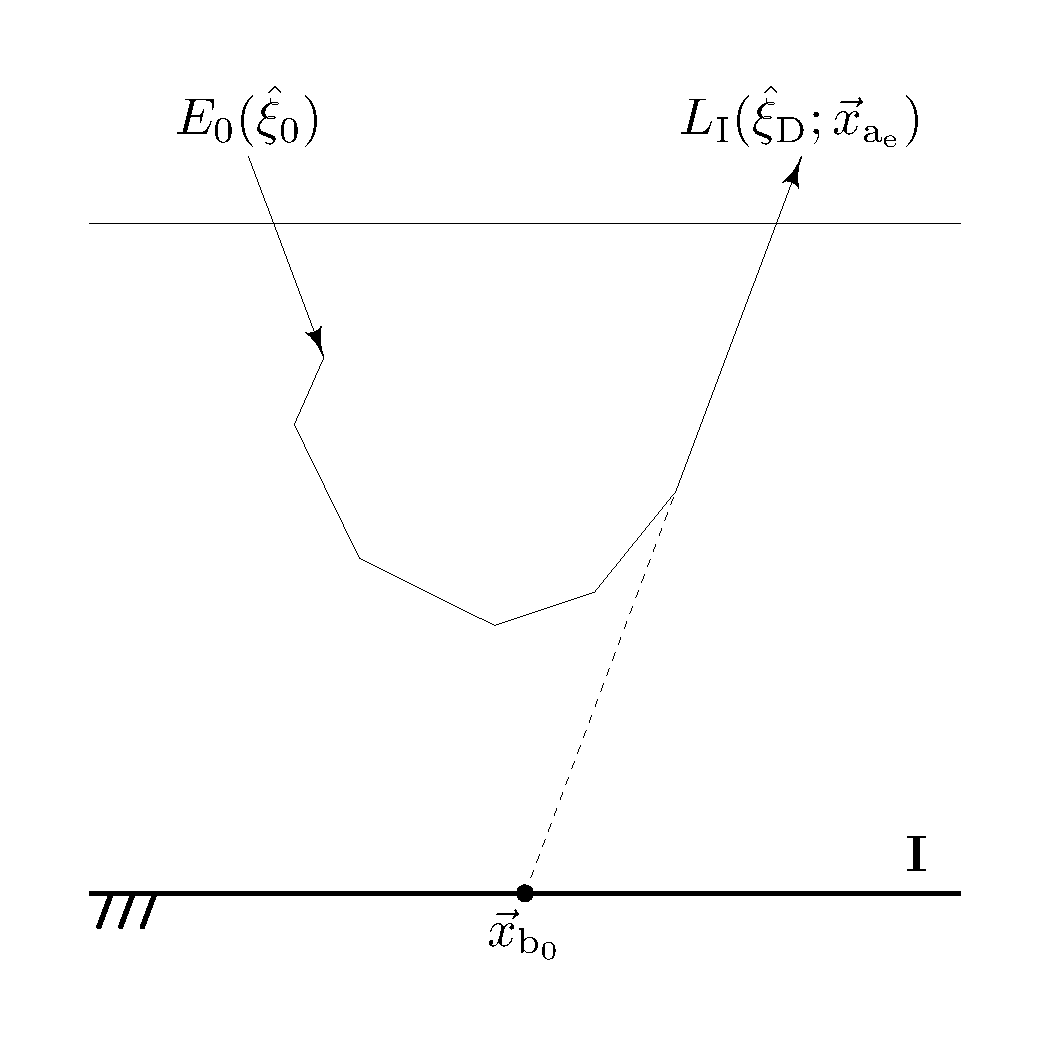
\includegraphics[width=0.35\linewidth]{components_A}
  \caption{Atmospheric signal component. Adapted from \citet{Tanre1979}.}
  \label{fig:theory_components_A}
\end{figure}

The component \textbf{I} represented in Fig.~\ref{fig:theory_components_A} corresponds to light rays that have not interacted with the surface. It is reflected by the atmosphere into the detector in direction $\smash{\hat{\xi}}_\text{D}$ when the atmosphere is illuminated from above by Sun rays from direction $\smash{\hat{\xi}_0}$:

\begin{equation}
L_\text{I}(\hat{\xi}_\text{D}; \vec{x}_{\text{a}_\text{e}}) = E_0(\hat{\xi}_0) \int\limits_{A} d\vec{x}_{\text{a}_\text{i}} \curlyvee_{\!\text{a}}\!(\hat{\xi}_0 \rightarrow \hat{\xi}_\text{D}; \vec{x}_{\text{a}_\text{i}} \rightarrow \vec{x}_{\text{a}_\text{e}}),
\label{eq:theory_comp_I_C0}
\end{equation}

\noindent where $\smash{L_\text{I}(\hat{\xi}_\text{D}; \vec{x}_{\text{a}_\text{e}})}$ is the radiance of component I reaching the detector, the subscripts ``i'' and ``e'' represent the position of incidence and the position of exitance, respectively, and the integral is taken over the TOA. The function $\smash{\curlyvee_{\!\text{a}}(\hat{\xi}^\prime \rightarrow \hat{\xi}; \vec{x}^{\, \prime} \rightarrow \vec{x})}$, with units of m$^{-2}$~sr$^{-1}$, is the bidirectional scattering-surface reflectance distribution function \citep[BSSRDF;][]{Venable1974,Nicodemus1977} of the atmosphere when illuminated from above.

As in our development the atmosphere is horizontally homogeneous, $\smash{\curlyvee_{\!\text{a}}(\hat{\xi}^\prime \rightarrow \hat{\xi}; \vec{x}^{\, \prime} \rightarrow \vec{x})}$ depends only on the distance between incidence and exitance and not on the specific positions, and Eq.~\ref{eq:theory_comp_I_C0} simplifies to:

\begin{equation}
L_\text{I}(\hat{\xi}_\text{D}; \vec{x}_{\text{a}_\text{e}}) = E_0(\hat{\xi}_0) \, \rho_\text{a}(\hat{\xi}_0 \rightarrow \hat{\xi}_\text{D}),
\label{eq:theory_comp_I_C1}
\end{equation}

\noindent where the function $\smash{\rho_\text{a}(\hat{\xi}^\prime \rightarrow \hat{\xi})}$, with units of sr$^{-1}$, is the bidirectional reflectance distribution function \citep[BRDF;][]{Nicodemus1977} of the atmosphere when illuminated from above, and it is given by:

\begin{equation}
\rho_\text{a}(\hat{\xi}^\prime \rightarrow \hat{\xi}) = \int\limits_{A} d\vec{x}^{\, \prime}  \curlyvee_{\!\text{a}}\!(\hat{\xi}^\prime \rightarrow \hat{\xi}; \vec{x} - \vec{x}^{\, \prime}).
\label{eq:theory_a_brdf}
\end{equation}

In our formulation, $\smash{\curlyvee_{\!\text{a}}(\hat{\xi}^\prime \rightarrow \hat{\xi}; \vec{x}^{\, \prime} \rightarrow \vec{x})}$, and consequently, $\smash{\rho_\text{a}(\hat{\xi}^\prime \rightarrow \hat{\xi})}$, includes all the effects of absorption and scattering (gaseous or particulate) occurring in the atmosphere. This will be the case for all atmospheric reflectance and transmittance functions in this chapter.
 
% Section -------------------------------------------------------------------
\section{Target surface signal}

\begin{figure}[!htbp]
  \centering
  \begin{subfigure}{0.35\linewidth}
  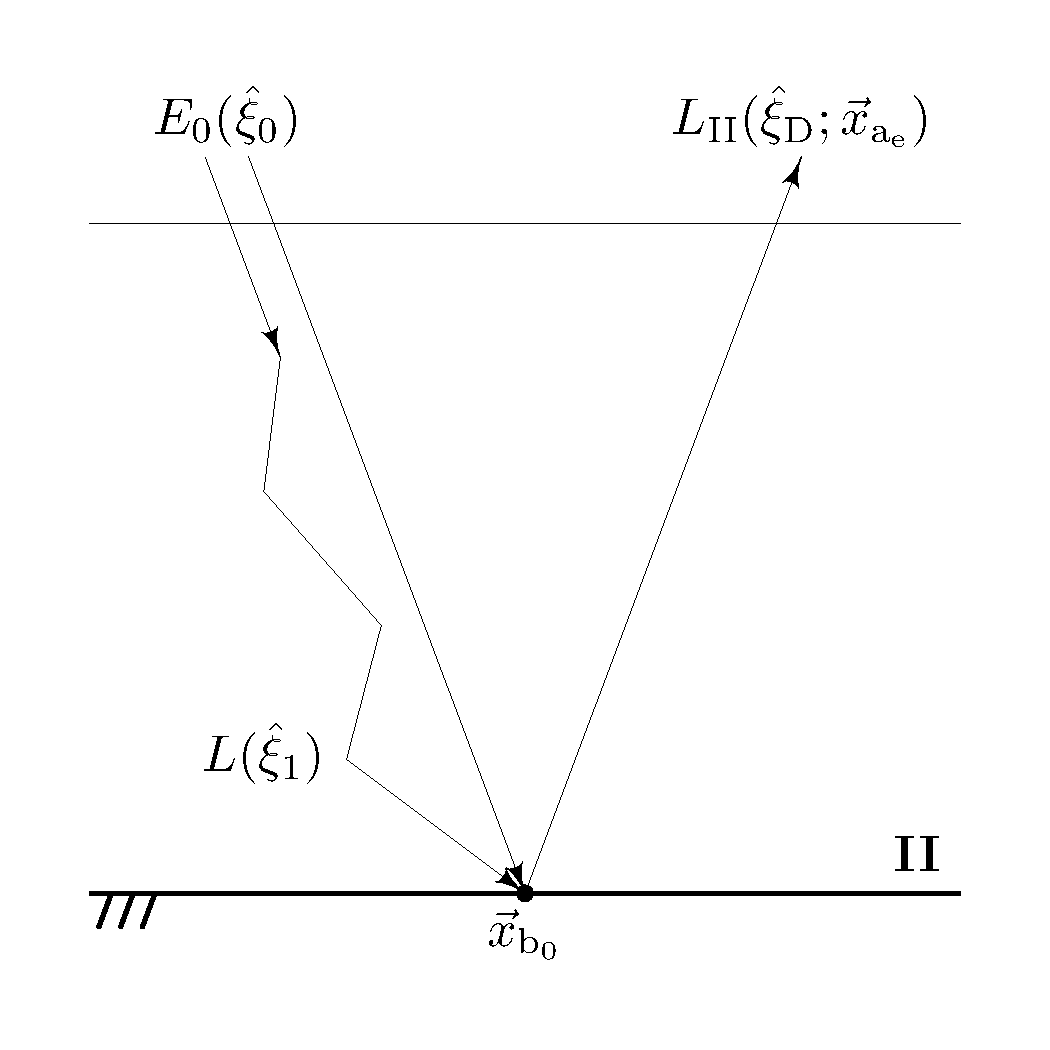
\includegraphics[width=\linewidth]{components_B}
  \end{subfigure}
  \begin{subfigure}{0.35\linewidth}
  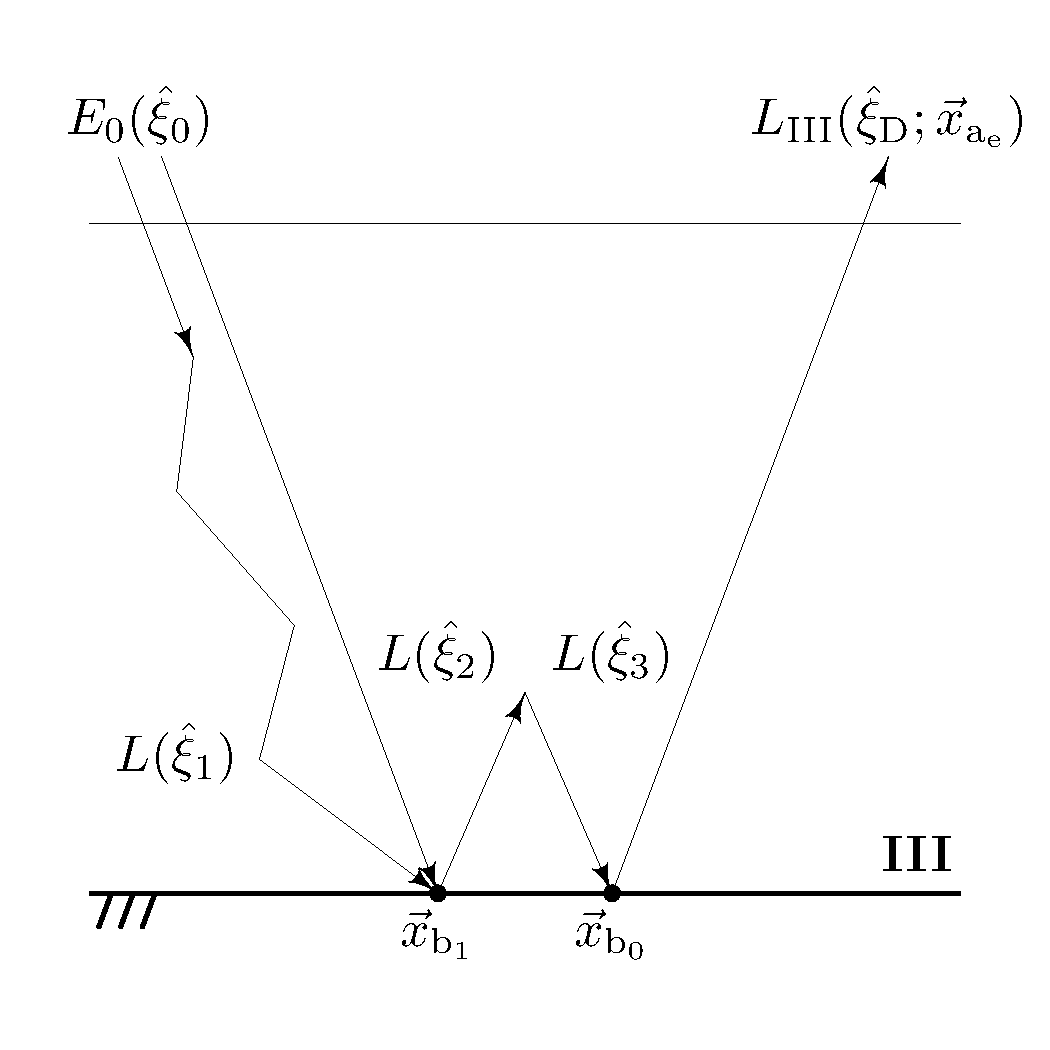
\includegraphics[width=\linewidth]{components_C}
  \end{subfigure}
  \caption{Target surface signal component. Adapted from \citet{Tanre1979}.}
  \label{fig:theory_components_BC}
\end{figure}

The components represented in Fig.~\ref{fig:theory_components_BC} carry the signal of the surface target directly transmitted to the sensor when illuminated by light with different scattering histories. Component \textbf{II} in Fig.~\ref{fig:theory_components_BC} corresponds to the light rays transmitted downwards through the atmosphere, reflected by the target surface at position $\smash{\vec{x}_{\text{b}_0}}$ and directly transmitted to the sensor when the surface is illuminated by light that has not yet interacted with the surface. It can be calculated as:

\begin{equation}
\openup 2\jot
\begin{split}
L_\text{II}(\hat{\xi}_\text{D}; \vec{x}_{\text{a}_\text{e}}) &= E_0(\hat{\xi}_0) \, T_{\text{u}_\text{dir}}(\hat{\xi}_\text{D}; \vec{x}_{\text{b}_0}) \\
&\times \Biggr\{ T_{\text{d}_\text{dir}}(\hat{\xi}_0; \vec{x}_{\text{a}_\text{i}}) \, \rho_\text{s}(\hat{\xi}_0 \rightarrow \hat{\xi}_\text{D}; \vec{x}_{\text{b}_0}) \\
&+ \int\limits_\hemidn d\Omega(\hat{\xi}_1) \, |\hat{\xi}_1 \cdot \hat{n}| \int\limits_{A} d\vec{x}_{\text{a}_\text{i}} \curlywedge_\text{a}^*\!(\hat{\xi}_0 \rightarrow \hat{\xi}_1; \vec{x}_{\text{a}_\text{i}} \rightarrow \vec{x}_{\text{b}_0}) \, \rho_\text{s}(\hat{\xi}_1 \rightarrow \hat{\xi}_\text{D}; \vec{x}_{\text{b}_0}) \Biggr\},
\end{split}
\label{eq:theory_comp_II_C0}
\end{equation} 

\noindent where $\smash{T_{\text{u}_\text{dir}}(\hat{\xi}_\text{D}; \vec{x}_{\text{b}_0})}$, unitless, is the upward direct transmittance in the direction of the detector, $\smash{T_{\text{d}_\text{dir}}(\hat{\xi}_0; \vec{x}_{\text{a}_\text{i}})}$, unitless, is the downward direct transmittance of the atmosphere for the incident Sun irradiance, $\smash{\rho_\text{s}(\hat{\xi}^\prime \rightarrow \hat{\xi}; \vec{x}_{\text{b}_0})}$ is the BRDF of the surface target, the function $\smash{\curlywedge_\text{a}^*(\hat{\xi}^\prime \rightarrow \hat{\xi}; \vec{x}^{\,\prime} \rightarrow \vec{x})}$, with units of m$^{-2}$~sr$^{-1}$, is the diffuse bidirectional scattering-surface transmittance distribution function (BSSTDF) of the atmosphere when illuminated from above, $\smash{d\Omega(\hat{\xi})}$ is an element of solid angle centred on direction $\smash{\hat{\xi}}$, and the integral is taken over all directions in the downward hemisphere, $\smash{\hemidn}$.

As in our development the atmosphere is defined to be horizontally homogeneous and the surface reflection functions to be isotropic, Eq.~\ref{eq:theory_comp_II_C0} simplifies to:

\begin{equation}
L_\text{II}(\hat{\xi}_\text{D}; \vec{x}_{\text{a}_\text{e}}) = E_0(\hat{\xi}_0) \, T_{\text{d}_\text{tot}}(\hat{\xi}_0 \rightarrow \hemidn) \, \rho_\text{s}(\vec{x}_{\text{b}_0})\, T_{\text{u}_\text{dir}}(\hat{\xi}_\text{D}),
\label{eq:theory_comp_II_C2}
\end{equation}

\noindent where:

\begin{equation}
T_{\text{d}_\text{tot}}(\hat{\xi}^\prime \rightarrow \hemidn) = T_{\text{d}_\text{dir}}(\hat{\xi}^\prime) + T_{\text{d}_\text{dif}}(\hat{\xi}^\prime \rightarrow \hemidn),
\label{eq:theory_tdtot}
\end{equation}
\begin{equation}
T_{\text{d}_\text{dif}}(\hat{\xi}^\prime \rightarrow \hemidn) = \int\limits_{A} d\vec{x}^{\, \prime} \int\limits_\hemidn d\Omega(\hat{\xi}) \, |\hat{\xi} \cdot \hat{n}| \, \!\curlywedge_\text{a}^*\!(\hat{\xi}^\prime \rightarrow \hat{\xi}; \vec{x} - \vec{x}^{\, \prime}),
\label{eq:theory_tddif}
\end{equation}

In Eq.~\ref{eq:theory_comp_II_C2} to Eq.~\ref{eq:theory_tddif}, the function $\smash{T_{\text{d}_\text{tot}}(\hat{\xi}^\prime \rightarrow \hemidn)}$, unitless, is the total downward transmittance of the atmosphere (or the downward directional-hemispherical transmittance), $\smash{T_{\text{d}_\text{dif}}(\hat{\xi}^\prime \rightarrow \hemidn)}$, unitless, is the diffuse downward transmittance of the atmosphere, and $\smash{\rho_\text{s}(\vec{x})}$, with units of sr$^{-1}$, can represent either the BRDF or the hemispherical-directional reflectance of the target surface, which are equal for Lambertian surfaces (\textit{cf.} Eq.~\ref{eq:theory_lambert}). Further, the direct transmittances $\smash{T_{\text{u}_\text{dir}}(\hat{\xi}^\prime)}$ in Eq.~\ref{eq:theory_comp_II_C2} and $\smash{T_{\text{d}_\text{dir}}(\hat{\xi}^\prime)}$ in Eq.~\ref{eq:theory_tdtot} are given by the attenuation law:

\begin{equation}
T_{\text{dir}}(\hat{\xi}^\prime) = \exp{\left(-\frac{\tau}{|\hat{\xi}^\prime \cdot \hat{n}|}\right)},
\label{eq:theory_tdir}
\end{equation}

\noindent where $\smash{\tau}$, unitless, is the optical depth of the atmosphere. Note that because of the specific conditions being represented, dependence of position in the atmosphere and direction in surface reflectances was dropped in the above equations.

The quantities involved in Eq.~\ref{eq:theory_comp_II_C2} cannot be measured directly from a remote platform and typically are not known for a general case. The reflectance of the target surface is unknown, while $\smash{T_{\text{d}_\text{tot}}(\hat{\xi}_0 \rightarrow \hemidn)}$ and $\smash{T_{\text{u}_\text{dir}}(\hat{\xi}_\text{D})}$ depend on the variable atmosphere composition and atmospheric pressure at the surface. 

The component \textbf{III} in Fig.~\ref{fig:theory_components_BC} corresponds to the light rays that were transmitted downward through the atmosphere, reflected by the target surface at position $\smash{\vec{x}_{\text{b}_0}}$ and directly transmitted to the sensor when illuminated by light that has interacted with the surface at least once. This component represents part of the contribution of the sperical albedo for the atmospheric blurring. The magnitude of this component depends on the multiple interaction between the reflectance of the surrounding surfaces and the atmosphere. We will first consider a single order of interaction between the surface and the atmosphere before considering the more general situation of multiple interactions. The radiance from the first interaction, $\smash{L_{\text{III}_\text{1}}(\hat{\xi}_\text{D})}$, can be calculated as:

\begin{equation}
\openup 2\jot
\begin{split}
L_{\text{III}_\text{1}}&(\hat{\xi}_\text{D}; \vec{x}_{\text{a}_\text{e}}) = E_0(\hat{\xi}_0) \, T_{\text{u}_\text{dir}}(\hat{\xi}_\text{D}; \vec{x}_{\text{b}_0}) \int\limits_B d\vec{x}_{\text{b}_1} \int\limits_{\hemidn} d\Omega(\hat{\xi}_3) \, |\hat{\xi}_3 \cdot \hat{n}| \int\limits_{\hemiup} d\Omega(\hat{\xi}_2) \, |\hat{\xi}_2 \cdot \hat{n}| \\
&\times \Biggr\{\Biggr[ T_{\text{d}_\text{dir}}(\hat{\xi}_0; \vec{x}_{\text{a}_\text{i}}) \, \rho_\text{s}(\hat{\xi}_0 \rightarrow \hat{\xi}_2; \vec{x}_{\text{b}_1}) \\
&+ \int\limits_\hemidn d\Omega(\hat{\xi}_1) \, |\hat{\xi}_1 \cdot \hat{n}| \int\limits_{A} d\vec{x}_{\text{a}_\text{i}} \!\curlywedge_\text{a}^*\!(\hat{\xi}_0 \rightarrow \hat{\xi}_1; \vec{x}_{\text{a}_\text{i}} \! \rightarrow \vec{x}_{\text{b}_1}) \, \rho_\text{s}(\hat{\xi}_1 \rightarrow \hat{\xi}_2; \vec{x}_{\text{b}_1}) \Biggr] \\
&\times \curlyvee_{\!\text{b}}(\hat{\xi}_2 \rightarrow \hat{\xi}_3; \vec{x}_{\text{b}_1} \!\rightarrow \vec{x}_{\text{b}_0}) \, \rho_\text{s}(\hat{\xi}_3 \rightarrow \hat{\xi}_\text{D}; \vec{x}_{\text{b}_0}) \Biggr\},
\end{split}
\label{eq:theory_comp_III_1_C0}
\end{equation} 

\noindent where $\smash{\curlyvee_{\!\text{b}}(\hat{\xi}^\prime \rightarrow \hat{\xi}; \vec{x}^{\, \prime} \rightarrow \vec{x})}$ is the BSSRDF of the atmosphere when illuminated from below (subscript ``b'' indicates incidence from the BOA), and $\smash{\hemiup}$ represents all directions in the upward hemisphere. The function $\smash{\curlyvee_{\!\text{b}}(\hat{\xi}^\prime \rightarrow \hat{\xi}; \vec{x}^{\, \prime}  \rightarrow \vec{x})}$ maps the contribution of light reflected in each direction from neighbouring surface elements to the energy reflected downwards by the atmosphere towards the target position. Its directional and spatial integral is the spherical albedo of the atmosphere.

As in our development the atmosphere is horizontally homogeneous and surface reflection functions are isotropic, Eq.~\ref{eq:theory_comp_III_1_C0} simplifies to:

\begin{equation}
\openup 2\jot
\begin{split}
L_{\text{III}_1}&(\hat{\xi}_\text{D}; \vec{x}_{\text{a}_\text{e}}) = E_0(\hat{\xi}_0) \, T_{\text{d}_\text{tot}}(\hat{\xi}_0 \rightarrow \hemidn) \, T_{\text{u}_\text{dir}}(\hat{\xi}_\text{D}) \, \rho_\text{s}(\vec{x}_{\text{b}_0}) \\
& \times \int\limits_B d\vec{x}_{\text{b}_1} \, \pi \, \rho_\text{s}(\vec{x}_{\text{b}_1}) \! \curlyvee_{\!\text{b}}\!(\hemiup \rightarrow \hemidn; \vec{x}_{\text{b}_0} \!- \vec{x}_{\text{b}_1}).
\end{split}
\label{eq:theory_comp_III_1_C2}
\end{equation}

\noindent where:

\begin{equation}
\curlyvee_{\!\text{b}}(\hemiup \rightarrow \hemidn; \vec{x} - \vec{x}^{\, \prime}) = \frac{1}{\pi} \int\limits_{\hemidn} d\Omega(\hat{\xi}) \, |\hat{\xi} \cdot \hat{n}| \int\limits_{\hemiup} d\Omega(\hat{\xi}^\prime) \, |\hat{\xi}^\prime \! \cdot \hat{n}| \! \curlyvee_{\!\text{b}}\!(\hat{\xi}^\prime \rightarrow \hat{\xi}; \vec{x} - \vec{x}^{\, \prime}).
\label{eq:theory_bsstdf_bh}
\end{equation}

In Eq.~\ref{eq:theory_comp_III_1_C2} and Eq.~\ref{eq:theory_bsstdf_bh}, $\smash{\curlyvee_{\!\text{b}}(\hemiup \rightarrow \hemidn; \vec{x} - \vec{x}^{\, \prime})}$, with units of m$^{-2}$, is the bi-hemispherical integral of the BSSRDF of the atmosphere when illuminated from below. $\smash{\curlyvee_{\!\text{b}}(\hemiup \rightarrow \hemidn; \vec{x} - \vec{x}^{\, \prime})}$ can be understood as the spatially-resolved spherical albedo and is further discussed in Chapter~\ref{ch:sph_albd}. The $\smash{\pi}$~sr factor appearing in the above equations is the projected solid angle integral of an hemisphere. For a Lambertian BRDF:

\begin{equation}
\frac{1}{\pi} \, \rho(\hemidn \rightarrow \hemiup; \vec{x}) = \rho(\hemidn \rightarrow \hat{\xi}; \vec{x}) = \rho(\hat{\xi}^\prime \rightarrow \hat{\xi}; \vec{x}) = \rho(\vec{x}).
\label{eq:theory_lambert}
\end{equation}

We note that the spatial integral in Eq.~\ref{eq:theory_comp_III_1_C2} is a convolution and can be presented in a more compact notation using the convolution operator, $\smash{\circledast}$:

\begin{equation}
\Bigr\{\pi \, \rho_\text{s}(\vec{x}^{\,\prime}) \circledast \! \curlyvee_{\!\text{b}}(\hemiup \rightarrow \hemidn; \vec{x}^{\,\prime})\Bigr\}(\vec{x}).
\label{eq:theory_bhem_conv}
\end{equation}

A single order or interaction would be a sufficient approximation for component $\smash{L_\text{III}(\hat{\xi}_\text{D}; \vec{x}_{\text{a}_\text{e}})}$ if the surface reflectances and the spherical albedo have a small magnitude. However this is not expected to hold under all conditions in which aquatic remote sensing is of interest, due to the spectrally and temporally variable optical properties of the atmosphere, water and land. The contribution of component \textbf{III} account for all orders of interaction is given by:

\begin{equation}
\openup 2\jot
\begin{split}
L_\text{III}&(\hat{\xi}_\text{D}; \vec{x}_{\text{a}_\text{e}}) = E_0(\hat{\xi}_0) \, T_{\text{d}_\text{tot}}(\hat{\xi}_0 \rightarrow \hemidn) \, T_{\text{u}_\text{dir}}(\hat{\xi}_\text{D}) \, \rho_\text{s}(\vec{x}_{\text{b}_0}) \\
& \times \sum\limits_{k = 1}^{\infty} \, \int\limits_B d^k\mathbf{x}_\text{b} \, \prod\limits_{j = 1}^{k} \, \pi \, \rho_\text{s}(\vec{x}_{\text{b}_j}) \! \curlyvee_{\!\text{b}}\!(\hemiup \rightarrow \hemidn; \vec{x}_{\text{b}_{j-1}} \!- \vec{x}_{\text{b}_j}),
\end{split}
\label{eq:theory_comp_III_all_C2}
\end{equation}

\noindent where $\smash{\sum}$ and $\smash{\prod}$ are the operators for the sum and product of a series, respectively, and $\smash{\mathbf{x}_\text{b}}$ includes all area elements $\smash{\vec{x}_{\text{b}_j}}$ from 1 to $k$. An alternative representation of this equation, substituting the integral, is given by:

\begin{equation}
\openup 2\jot
\begin{split}
L_\text{III}&(\hat{\xi}_\text{D}; \vec{x}_{\text{a}_\text{e}}) = E_0(\hat{\xi}_0) \, T_{\text{d}_\text{tot}}(\hat{\xi}_0 \rightarrow \hemidn) \, T_{\text{u}_\text{dir}}(\hat{\xi}_\text{D}) \, \rho_\text{s}(\vec{x}_{\text{b}_0}) \\
& \times \sum\limits_{k = 1}^{\infty} \, \rho_\text{b}(\hemiup \rightarrow \hemidn)^k \, \prod\limits_{j = 1}^{k} \, \rho_{\text{s}_{\curlyvee_\text{b}}}(\hemidn \rightarrow \hemiup; \vec{x}_{\text{b}_{j-1}}),
\end{split}
\label{eq:theory_comp_III_all_C2B}
\end{equation}

where:

\begin{equation}
\rho_{\text{s}_{\curlyvee_\text{b}}}(\hemidn \rightarrow \hemiup; \vec{x}_{\text{b}_{j-1}}) = \frac{1}{\rho_\text{b}(\hemiup \rightarrow \hemidn)^j} \int\limits_B d^j\mathbf{x}_\text{b} \, \prod\limits_{i = 1}^{j} \, \pi \, \rho_\text{s}(\vec{x}_{\text{b}_i}) \! \curlyvee_{\!\text{b}}\!(\hemiup \rightarrow \hemidn; \vec{x}_{\text{b}_{i-1}} - \vec{x}_{\text{b}_i}),
\label{eq:theory_bhem}
\end{equation}

and

\begin{equation}
\rho_\text{b}(\hemiup \rightarrow \hemidn) = \int\limits_B d\vec{x}^{\, \prime} \curlyvee_{\!\text{b}}\!(\hemiup \rightarrow \hemidn; \vec{x} - \vec{x}^{\, \prime}).
\label{eq:theory_sa}
\end{equation}

In Eq.~\ref{eq:theory_comp_III_all_C2B} to Eq.~\ref{eq:theory_sa}, the function $\smash{\rho_{\text{s}_{\curlyvee_\text{b}}}(\hemidn \rightarrow \hemiup; \vec{x}_{\text{b}_{j-1}})}$, unitless, is the weighted average bi-hemispherical reflectance of the surfaces surrounding $\smash{\vec{x}_{\text{b}_{j-1}}}$ that contribute to the downwelling radiance $\smash{L(\hat{\xi}_{j+2})}$ (\textit{cf.} Fig.~\ref{fig:theory_components_BC}), and the function $\smash{\rho_\text{b}(\hemiup \rightarrow \hemidn)}$, unitless, is the bi-hemispherical reflectance of the atmosphere when illuminated from below (also known as spherical albedo).

Further simplification of Eq.~\ref{eq:theory_comp_III_all_C2B} is possible with the assumption that the weighted average bi-hemispherical reflectance of the surfaces surrounding $\smash{\vec{x}_{\text{b}_{j-1}}}$ is approximately equal to $\smash{\rho_{\text{s}_{\curlyvee_\text{b}}}(\hemidn \rightarrow \hemiup; \vec{x}_{\text{b}_0})}$. As it will be shown in Chapter~\ref{ch:sph_albd} and Appendix~\ref{ap:apsfs}, the magnitude, spatial scale and radial profile of the spherical albedo is such that this is a reasonable assumption except at very high aerosol optical thickness ($>>1$). That is, the BSSRDF of the atmosphere when illuminated from below causes high blurring of the surface reflectance pattern and its contribution from high orders of interaction and positions distant from $\vec{x}_{\text{b}_0}$ is negligible. Under this approximation, Eq.~\ref{eq:theory_comp_III_all_C2B} simplifies to:

\begin{equation}
\openup 2\jot
\begin{split}
L_\text{III}&(\hat{\xi}_\text{D}; \vec{x}_{\text{a}_\text{e}}) = E_0(\hat{\xi}_0) \, T_{\text{d}_\text{tot}}(\hat{\xi}_0 \rightarrow \hemidn) \, T_{\text{u}_\text{dir}}(\hat{\xi}_\text{D}) \, \rho_\text{s}(\vec{x}_{\text{b}_0}) \\
& \times \sum\limits_{k = 1}^{\infty} \Bigr\{ \rho_\text{b}(\hemiup \rightarrow \hemidn) \, \rho_{\text{s}_{\curlyvee_\text{b}}}(\hemidn \rightarrow \hemiup; \vec{x}_{\text{b}_0})\Bigr\}^k.
\end{split}
\label{eq:theory_comp_III_all_C2C}
\end{equation}

\hfill \break

Combining components \textbf{II} and \textbf{III} we have:

\begin{equation}
\openup 2\jot
\begin{split}
L_\text{II+III}&(\hat{\xi}_\text{D}; \vec{x}_{\text{a}_\text{e}}) \\
&= E_0(\hat{\xi}_0) \, T_{\text{d}_\text{tot}}(\hat{\xi}_0 \rightarrow \hemidn) \, \rho_\text{s}(\vec{x}_{\text{b}_0}) \, T_{\text{u}_\text{dir}}(\hat{\xi}_\text{D}) \, \sum\limits_{k = 0}^{\infty} \Bigr\{ \rho_\text{b}(\hemiup \rightarrow \hemidn) \, \rho_{\text{s}_{\curlyvee_\text{b}}}(\hemidn \rightarrow \hemiup; \vec{x}_{\text{b}_0})\Bigr\}^k \\
& = E_0(\hat{\xi}_0) \, T_{\text{d}_\text{tot}}(\hat{\xi}_0 \rightarrow \hemidn) \, \frac{\rho_\text{s}(\vec{x}_{\text{b}_0})}{1- \rho_\text{b}(\hemiup \rightarrow \hemidn) \, \rho_{\text{s}_{\curlyvee_\text{b}}}(\hemidn \rightarrow \hemiup; \vec{x}_{\text{b}_0})} \, T_{\text{u}_\text{dir}}(\hat{\xi}_\text{D}).
\end{split}
\label{eq:theory_comp_II_III_C2}
\end{equation}

The closed form in the right hand side of Eq.~\ref{eq:theory_comp_II_III_C2} is possible because the base of the geometric series evaluates to a value between 0 and 1, and the series converges. 

Before presenting the environmental signal, it is convenient to provide an alternative representation of Eq.~\ref{eq:theory_comp_II_III_C2}, by representing the direct upward transmission in the BSSTDF formalism:

\begin{equation}
\curlywedge_\text{b}^\cdot(\hat{\xi}^\prime \rightarrow \hat{\xi}; \vec{x} - \vec{x}^{\,\prime}) = \frac{1}{|\hat{\xi}^\prime \cdot \hat{n}|} \, T_{\text{u}_\text{dir}}(\hat{\xi}) \, \delta(\hat{\xi}^\prime-\hat{\xi}) \, \delta(\vec{x}^\prime - \vec{x}),
\label{eq:theory_tudir_pulse_dd}
\end{equation}
\begin{equation}
\begin{split}
\curlywedge_\text{b}^\cdot(\hemiup \rightarrow \hat{\xi}; \vec{x} - \vec{x}^{\,\prime}) &= \frac{1}{\pi} \, \int\limits_{\hemiup} d\Omega(\hat{\xi}^\prime) \, |\hat{\xi}^\prime \cdot \hat{n}| \curlywedge_\text{b}^\cdot(\hat{\xi}^\prime \rightarrow \hat{\xi}; \vec{x} - \vec{x}^{\,\prime}) \\
&= \frac{1}{\pi} \, \int\limits_{\hemiup} d\Omega(\hat{\xi}^\prime) \, T_{\text{u}_\text{dir}}(\hat{\xi}) \, \delta(\hat{\xi}^\prime-\hat{\xi}) \, \delta(\vec{x}^\prime - \vec{x}) \\
&= \frac{1}{\pi} \, T_{\text{u}_\text{dir}}(\hat{\xi}) \, \delta(\vec{x}^\prime - \vec{x})
\end{split}
\label{eq:theory_tudir_pulse_d}
\end{equation}

where $\smash{\delta}$ are Dirac delta functions on directions (with units of sr$^{-1}$), and on positions (with units of m$^{-2}$). Note that the superscript $^\cdot$ is used for this direct component, while the superscript $^*$ was used for the diffuse component. The functions 
$\smash{\curlywedge_\text{b}^\cdot(\hat{\xi}^\prime \rightarrow \hat{\xi}; \vec{x} - \vec{x}^{\,\prime})}$, with units of m$^{-2}$~sr$^{-1}$, is only non-zero in the direction $\smash{\hat{\xi}^\prime}$ and position $\smash{\vec{x}^{\,\prime}}$. Its integral over the incident hemisphere, $\smash{\curlywedge_\text{b}^\cdot(\hemiup \rightarrow \hat{\xi}; \vec{x} - \vec{x}^{\,\prime})}$, also with units of m$^{-2}$~sr$^{-1}$, is only non-zero in the position $\smash{\vec{x}^{\,\prime}}$.

Inserting Eq.~\ref{eq:theory_tudir_pulse_d} in Eq.~\ref{eq:theory_comp_II_III_C2} and using the convolution notation, we have (\textit{cf.} Eq.~\ref{eq:theory_bhem_conv}, \ref{eq:theory_bhem}, and \ref{eq:theory_sa}):

\begin{equation}
\openup 2\jot
\begin{split}
L_\text{II+III}&(\hat{\xi}_\text{D}; \vec{x}_\text{a}) = E_0(\hat{\xi}_0) \, T_{\text{d}_\text{tot}}(\hat{\xi}_0 \rightarrow \hemidn) \\
& \times \,\Biggl\{\frac{\pi \, \rho_\text{s}(\vec{x}^{\,\prime})}{1 - \bigl\{\pi \, \rho_\text{s}(\vec{x}^{\,\prime\prime}) \circledast \! \curlyvee_{\!\text{b}}(\hemiup \rightarrow \hemidn; \vec{x}^{\,\prime\prime})\bigl\}(\vec{x}^{\,\prime})} \circledast \curlywedge_\text{b}^\cdot(\hemiup \rightarrow \hat{\xi}_\text{D};\vec{x}^{\,\prime}) \Biggl\}(\vec{x}_{\text{a}_\text{e}}).
\end{split}
\label{eq:theory_comp_II_III_C2_pulse}
\end{equation}

\hfill \break

% Section -------------------------------------------------------------------
\section{Environmental signal}

\begin{figure}[!htbp]
  \centering
  \begin{subfigure}{0.35\linewidth}
  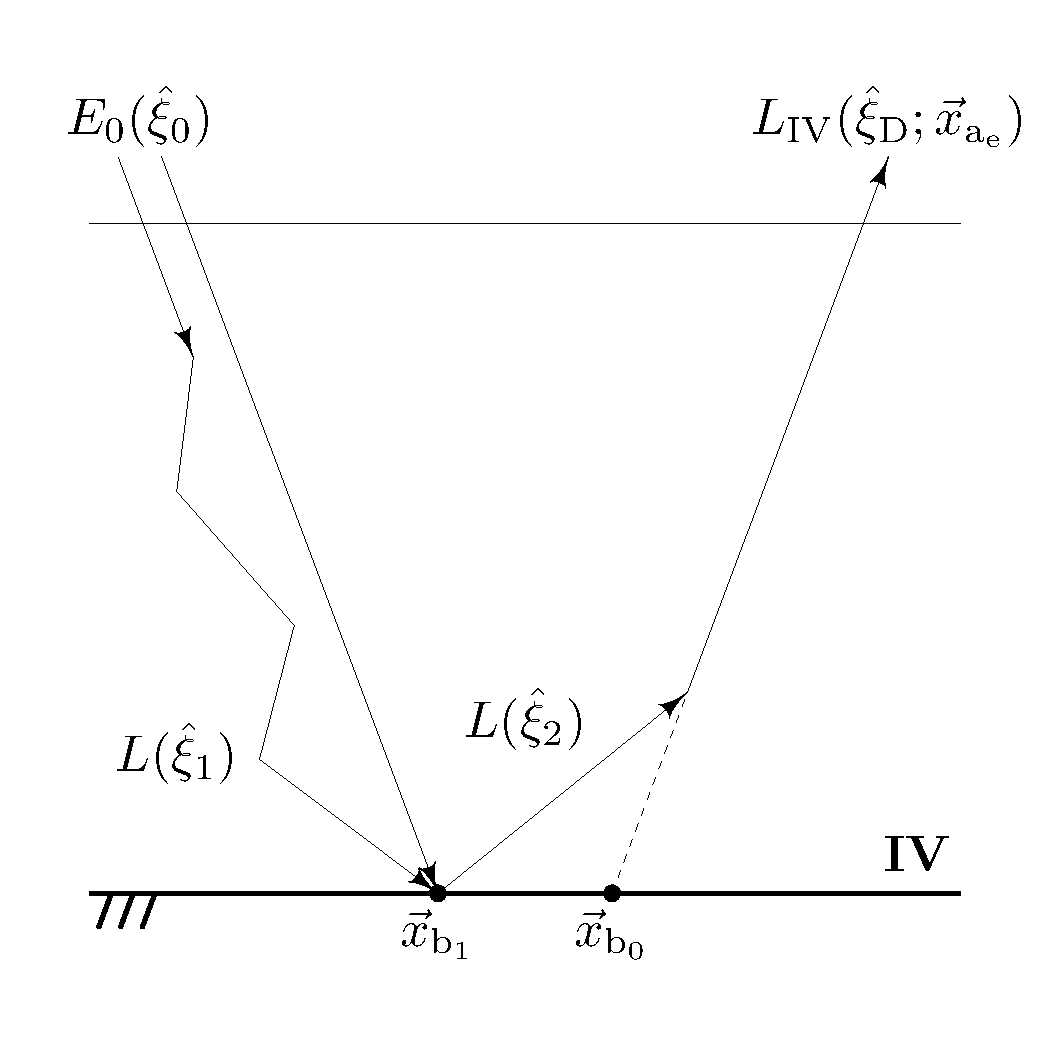
\includegraphics[width=\linewidth]{components_D}
  \end{subfigure}
  \begin{subfigure}{0.35\linewidth}
  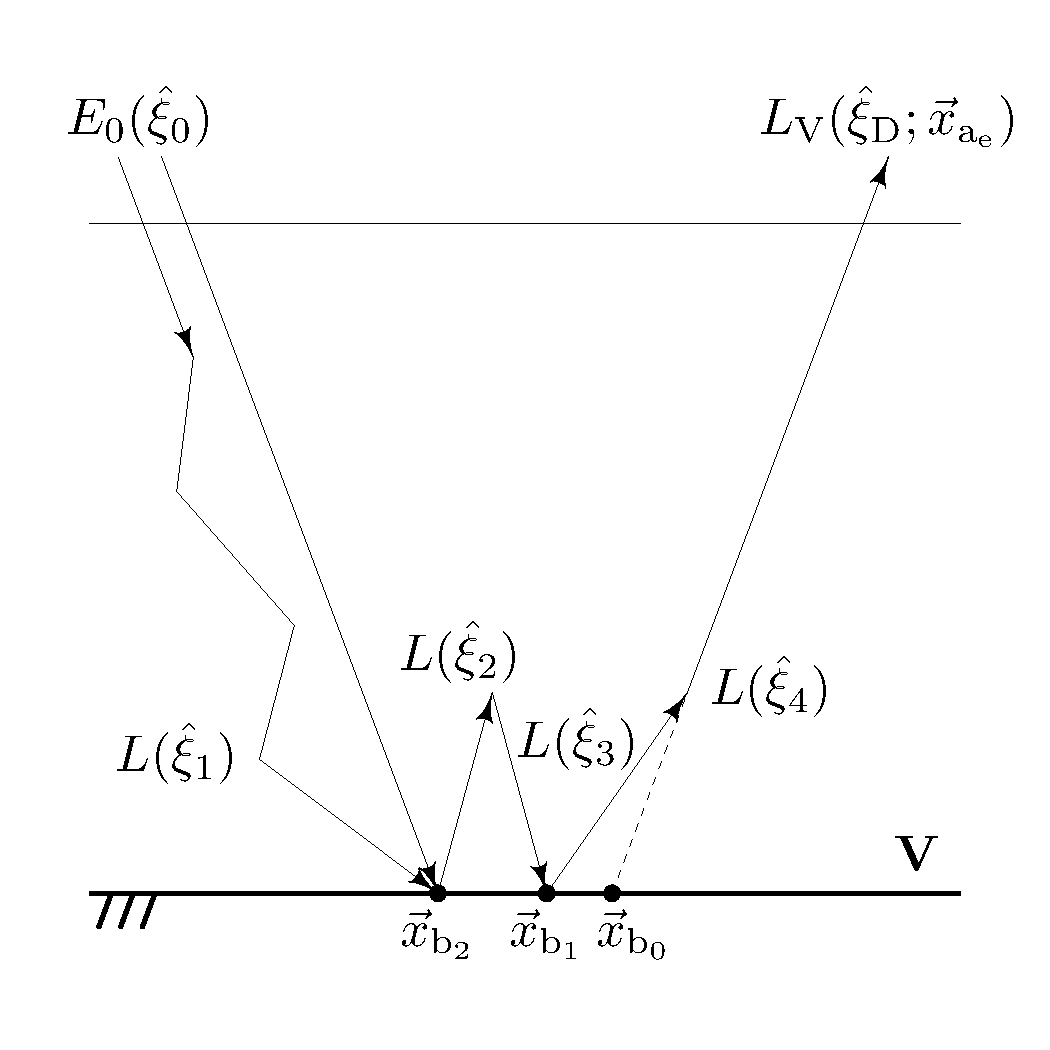
\includegraphics[width=\linewidth]{components_E}
  \end{subfigure}
  \caption{Surrounding surfaces signal component. Adapted from \citet{Tanre1979}.}
  \label{fig:theory_components_DE}
\end{figure}

The final components, represented in Fig.~\ref{fig:theory_components_DE}, correspond to the environmental surface signal, \textit{i.e.} the signal reflected by surrounding surfaces and diffusely transmitted to the sensor. The formulation of component \textbf{IV} in Fig.~\ref{fig:theory_components_DE} is similar to that of Eq.~\ref{eq:theory_comp_II_C2}, but substituting the direct transmittance of the target surface reflectance when illuminated by light that has not interacted with the surface, $\smash{\rho_\text{s}(\hemidn \rightarrow \hat{\xi}_\text{D}; \vec{x}_{\text{b}_0}) \, T_{\text{u}_\text{dir}}(\hat{\xi}_\text{D})}$, by the diffuse transmittance of the environmental reflectance surrounding the target. Specifically, component \textbf{IV} can be calculated as:

\begin{equation}
\openup 2\jot
\begin{split}
L_\text{IV}&(\hat{\xi}_\text{D}; \vec{x}_{\text{a}_\text{e}}) = E_0(\hat{\xi}_0) \, \int\limits_{B} d\vec{x}_{\text{b}_1} \int\limits_{\hemiup} d\Omega(\hat{\xi}_2) \, |\hat{\xi}_2 \cdot \hat{n}| \\
&\times \Biggr\{ \, T_{\text{d}_\text{dir}}(\hat{\xi}_0; \vec{x}_{\text{a}_\text{i}}) \, \rho_\text{s}(\hat{\xi}_0 \rightarrow \hat{\xi}_2; \vec{x}_{\text{b}_1})  \\
& + \int\limits_\hemidn d\Omega(\hat{\xi}_1) \, |\hat{\xi}_1 \cdot \hat{n}| \int\limits_A d\vec{x}_{\text{a}_\text{i}} \curlywedge_\text{a}^*\!(\hat{\xi}_0 \rightarrow \hat{\xi}_1; \vec{x}_{\text{a}_\text{i}} \rightarrow \vec{x}_{\text{b}_1}) \, \rho_\text{s}(\hat{\xi}_1 \rightarrow \hat{\xi}_2; \vec{x}_{\text{b}_1}) \Biggr\} \\
& \times \curlywedge_\text{b}^*(\hat{\xi}_2 \rightarrow \hat{\xi}_\text{D}; \vec{x}_{\text{b}_1} \rightarrow \vec{x}_{\text{a}_\text{e}}),
\end{split}
\label{eq:theory_comp_IV_C0}
\end{equation}

where $\smash{\curlywedge_\text{b}^*(\hat{\xi}^\prime \rightarrow \hat{\xi}; \vec{x}^{\,\prime} \rightarrow \vec{x})}$, with units of m$^{-2}$~sr$^{-1}$, is the atmospheric diffuse BSSTDF when illuminated from below.

As in our development the atmosphere is horizontally homogeneous and surface reflection functions are isotropic, Eq.~\ref{eq:theory_comp_IV_C0} simplifies to:

\begin{equation}
L_\text{IV}(\hat{\xi}_\text{D}; \vec{x}_{\text{a}_\text{e}}) = E_0(\hat{\xi}_0) \, T_{\text{d}_\text{tot}}(\hat{\xi}_0 \rightarrow \hemidn)  \, \rho_{\text{s}_{\curlywedge_\text{b}^*}}(\hemidn \rightarrow \hemiup; \vec{x}_{\text{b}_0}) \, T_{\text{u}_\text{dif}}(\hemiup \rightarrow \hat{\xi}_\text{D}),
\label{eq:theory_comp_IV_C2}
\end{equation}

\noindent where:

\begin{equation}
T_{\text{u}_\text{dif}}(\hemiup \rightarrow \hat{\xi}) = \int\limits_{B} d\vec{x}^{\, \prime} \curlywedge_\text{b}^*\!(\hemiup \rightarrow \hat{\xi}_\text{D}; \vec{x} - \vec{x}^{\, \prime}),
\label{eq:theory_tudif}
\end{equation}

\begin{equation}
\rho_{\text{s}_{\curlywedge_\text{b}^*}}(\hemidn \rightarrow \hemiup; \vec{x}_{\text{b}_0}) = \frac{1}{T_{\text{u}_\text{dif}}(\hemiup \rightarrow \hat{\xi})} \, \int\limits_{B} d\vec{x}_{\text{b}_1} \, \pi \, \rho_\text{s}(\vec{x}_{\text{b}_1}) \curlywedge_\text{b}^*\!(\hemiup \rightarrow \hat{\xi}_\text{D}; \vec{x}_{\text{a}_\text{e}} \! - \vec{x}_{\text{b}_1}),
\label{eq:theory_rho_psf}
\end{equation}

\noindent and

\begin{equation}
\curlywedge_\text{b}^*(\hemiup \rightarrow \hat{\xi}; \vec{x} - \vec{x}^{\, \prime}) = \frac{1}{\pi}\int\limits_{\hemiup} d\Omega(\hat{\xi}^\prime) \, |\hat{\xi}^\prime \!\cdot \hat{n}| \curlywedge_\text{b}^*\!(\hat{\xi}^\prime \rightarrow \hat{\xi}; \vec{x} - \vec{x}^{\, \prime}).
\label{eq:theory_bsstdf_hd}
\end{equation}

The integral over the incident hemisphere of the diffuse BSSTDF of the atmosphere when illuminated from below, $\smash{\curlywedge_\text{b}^*(\hemiup \rightarrow \hat{\xi}; \vec{x} - \vec{x}^{\, \prime})}$, with units of m$^{-2}$~sr$^{-1}$, is known as the the diffuse point spread function (PSF). The atmospheric PSF is further discussed in Chapter~\ref{ch:psf}. $\smash{T_{\text{u}_\text{dif}}(\hemiup \rightarrow \hat{\xi})}$, with units of sr$^{-1}$, is the upward hemispherical-directional diffuse transmittance of the atmosphere, and can be alternatively calculated as the incident average of the diffuse BTDF of the atmosphere when illuminated from below, $\smash{T_{\text{u}_\text{dif}}(\hat{\xi}^\prime \rightarrow \hat{\xi})}$, with units of sr$^{-1}$. For completeness, it should be noted that $\smash{T_{\text{u}_\text{dif}}(\hemiup \rightarrow \hat{\xi})}$ is related to the more common upward diffuse transmittance of the atmosphere, $\smash{T_{\text{u}_\text{dif}}(\hemiup \rightarrow \hemiup)}$, unitless, by $\smash{T_{\text{u}_\text{dif}}(\hemiup \rightarrow \hemiup) = \pi \, T_{\text{u}_\text{dif}}(\hemiup \rightarrow \hat{\xi})}$, assuming that $\smash{T_{\text{u}_\text{dif}}(\hemiup \rightarrow \hat{\xi})}$ is isotropic.

As it was done for Eq.~\ref{eq:theory_comp_III_1_C2}, the convolution in Eq.~\ref{eq:theory_rho_psf} can be more conveniently represented as:

\begin{equation}
\Bigr\{\pi \rho_\text{s}(\vec{x}^{\,\prime}) \circledast \! \curlywedge_\text{b}^*(\hemiup \rightarrow \hat{\xi}; \vec{x}^{\, \prime})\Bigr\}(\vec{x}).
\label{eq:theory_comp_IV_C2_conv}
\end{equation}

The last component, component \textbf{V} in Fig.~\ref{fig:theory_components_DE}, has the general development of Eq.~\ref{eq:theory_comp_III_1_C2}, but substituting the direct transmittance of the target surface reflectance when illuminated by light that has interacted with the surface at least once, $\smash{\rho_{\text{s}_2}(\hemidn \rightarrow \hat{\xi}_\text{D}; \vec{x}_{\text{b}_0}) \, T_{\text{u}_\text{dir}}(\hat{\xi}_\text{D})}$, by the diffuse transmittance of the environmental reflectance surrounding the target. Here again we start by considering the first order of interaction:

\begin{equation}
\openup 2\jot
\begin{split}
L_{\text{V}_\text{1}}&(\hat{\xi}_\text{D}; \vec{x}_{\text{a}_\text{e}}) = E_0(\hat{\xi}_0) \, \int\limits_B d\vec{x}_{\text{b}_2} \, \int\limits_{\hemidn} d\Omega(\hat{\xi}_4) \, |\hat{\xi}_4 \cdot \hat{n}| \\
&\times \int\limits_B d\vec{x}_{\text{b}_1}  \, \int\limits_{\hemidn} d\Omega(\hat{\xi}_3) \, |\hat{\xi}_3 \cdot \hat{n}| \, \int\limits_{\hemiup} d\Omega(\hat{\xi}_2) \, |\hat{\xi}_2 \cdot \hat{n}| \\
&\times \Biggr\{ \Biggr[ T_{\text{d}_\text{dir}}(\hat{\xi}_0; \vec{x}_{\text{a}_\text{i}}) \, \rho_\text{s}(\hat{\xi}_0 \rightarrow \hat{\xi}_2; \vec{x}_{\text{b}_1}) \\
& + \int\limits_\hemidn d\Omega(\hat{\xi}_1) \, |\hat{\xi}_1 \cdot \hat{n}| \int\limits_A d\vec{x}_{\text{a}_\text{i}} \curlywedge_\text{a}^*\!(\hat{\xi}_0 \rightarrow \hat{\xi}_1; \vec{x}_{\text{a}_\text{i}} \rightarrow \vec{x}_{\text{b}_1}) \, \rho_\text{s}(\hat{\xi}_1 \rightarrow \hat{\xi}_2; \vec{x}_{\text{b}_1})\Biggr] \\
&\times \curlyvee_\text{b}(\hat{\xi}_2 \rightarrow \hat{\xi}_3; \vec{x}_{\text{b}_1} \rightarrow \vec{x}_{\text{b}_2}) \, \rho_\text{s}(\hat{\xi}_3 \rightarrow \hat{\xi}_4; \vec{x}_{\text{b}_2}) \Biggr\} \curlywedge_\text{b}^*\!(\hat{\xi}_4 \rightarrow \hat{\xi}_\text{D}; \vec{x}_{\text{b}_2} \rightarrow \vec{x}_{\text{a}_\text{e}}).
\end{split}
\label{eq:theory_comp_V_1_C0}
\end{equation} 

The inner part is similar to Eq.~\ref{eq:theory_comp_III_1_C0} and since in our development the atmosphere is horizontally homogeneous and surface reflection functions are isotropic, the inner part is similar to Eq.~\ref{eq:theory_comp_III_1_C2}. Eq.~\ref{eq:theory_comp_V_1_C0} can then be represented as:

\begin{equation}
\openup 2\jot
\begin{split}
L_{\text{V}_\text{1}}&(\hat{\xi}_\text{D}; \vec{x}_{\text{a}_\text{e}}) = E_0(\hat{\xi}_0) \, T_{\text{d}_\text{tot}}(\hat{\xi}_0 \rightarrow \hemidn) \int\limits_B d\vec{x}_{\text{b}_1} \! \curlywedge_\text{b}^*(\hemiup \rightarrow \hat{\xi}_\text{D}; \vec{x}_{\text{a}_\text{e}} - \vec{x}_{\text{b}_1}) \, \pi \, \rho_\text{s}(\vec{x}_{\text{b}_1}) \\
&\times \rho_{\text{s}_{\curlyvee_\text{b}}}(\hemidn \rightarrow \hemiup; \vec{x}_{\text{b}_1}) \, \rho_\text{b}(\hemiup \rightarrow \hemidn) .
\end{split}
\label{eq:theory_comp_V_1_C2}
\end{equation} 

As it was done for Eq.~\ref{eq:theory_comp_III_all_C2C}, Eq.~\ref{eq:theory_comp_V_1_C2} can be generalized to include all orders of interaction:

\begin{equation}
\openup 2\jot
\begin{split}
L_\text{V}&(\hat{\xi}_\text{D}; \vec{x}_{\text{a}_\text{e}}) = E_0(\hat{\xi}_0) \, T_{\text{d}_\text{tot}}(\hat{\xi}_0 \rightarrow \hemidn) \int\limits_B d\vec{x}_{\text{b}_1} \! \curlywedge_\text{b}^*(\hemiup \rightarrow \hat{\xi}_\text{D}; \vec{x}_{\text{a}_\text{e}} - \vec{x}_{\text{b}_1}) \, \pi \, \rho_\text{s}(\vec{x}_{\text{b}_1}) \\
&\times \sum\limits_{k = 1}^{\infty} \Bigr\{ \rho_\text{b}(\hemiup \rightarrow \hemidn) \, \rho_{\text{s}_{\curlyvee_\text{b}}}(\hemidn \rightarrow \hemiup; \vec{x}_{\text{b}_1})\Bigr\}^k.
\end{split}
\label{eq:theory_comp_V_1_C2B}
\end{equation} 

To reach Eq.~\ref{eq:theory_comp_V_1_C2B}, the same assumption was made about $\smash{\rho_{\text{s}_{\curlyvee_\text{b}}}(\hemidn \rightarrow \hemiup; \vec{x}_{\text{b}})}$ as in the development of Eq.~\ref{eq:theory_comp_III_all_C2C}. And combining components IV and V, we have:

\begin{equation}
\openup 2\jot
\begin{split}
L_\text{IV + V}&(\hat{\xi}_\text{D}; \vec{x}_{\text{a}_\text{e}}) = E_0(\hat{\xi}_0) \, T_{\text{d}_\text{tot}}(\hat{\xi}_0 \rightarrow \hemidn) \int\limits_B d\vec{x}_{\text{b}_1} \! \curlywedge_\text{b}^*(\hemiup \rightarrow \hat{\xi}_\text{D}; \vec{x}_{\text{a}_\text{e}} - \vec{x}_{\text{b}_1}) \, \pi \, \rho_\text{s}(\vec{x}_{\text{b}_1}) \\
&\times \sum\limits_{k = 0}^{\infty} \Bigr\{ \rho_\text{b}(\hemiup \rightarrow \hemidn) \, \rho_{\text{s}_{\curlyvee_\text{b}}}(\hemidn \rightarrow \hemiup; \vec{x}_{\text{b}_1})\Bigr\}^k. \\
\therefore \\
L_\text{IV + V}&(\hat{\xi}_\text{D}; \vec{x}_{\text{a}_\text{e}}) = E_0(\hat{\xi}_0) \, T_{\text{d}_\text{tot}}(\hat{\xi}_0 \rightarrow \hemidn) \\
& \times \int\limits_B d\vec{x}_{\text{b}_1} \, \frac{\pi \, \rho_\text{s}(\vec{x}_{\text{b}_1})}{1 - \rho_\text{b}(\hemiup \rightarrow \hemidn) \, \rho_{\text{s}_{\curlyvee_\text{b}}}(\hemidn \rightarrow \hemiup; \vec{x}_{\text{b}_1})} \, \curlywedge_\text{b}^*(\hemiup \rightarrow \hat{\xi}_\text{D}; \vec{x}_{\text{a}_\text{e}} - \vec{x}_{\text{b}_1}).
\end{split}
\label{eq:theory_comp_IV_V_C2}
\end{equation} 

Finally, we can represent Eq.~\ref{eq:theory_comp_IV_V_C2} using the convolution notation with:

\begin{equation}
\openup 2\jot
\begin{split}
L_\text{IV + V}&(\hat{\xi}_\text{D}; \vec{x}_{\text{a}_\text{e}}) = E_0(\hat{\xi}_0) \, T_{\text{d}_\text{tot}}(\hat{\xi}_0 \rightarrow \hemidn) \\
& \times \,\Biggl\{\frac{\pi \, \rho_\text{s}(\vec{x}^{\,\prime})}{1 - \bigl\{\pi \, \rho_\text{s}(\vec{x}^{\,\prime\prime}) \circledast \! \curlyvee_{\!\text{b}}(\hemiup \rightarrow \hemidn; \vec{x}^{\,\prime\prime})\bigl\}(\vec{x}^{\,\prime})} \circledast \curlywedge_\text{b}^*(\hemiup \rightarrow \hat{\xi}_\text{D};\vec{x}^{\,\prime}) \Biggl\}(\vec{x}_{\text{a}_\text{e}}).
\end{split}
\label{eq:theory_comp_IV_V_C2_conv}
\end{equation} 

\hfill\break

% Section -------------------------------------------------------------------
\section{The ME over Lambertian surfaces}

Combining the five components developed previously, while transitioning from calculations for the target surface, $\smash{\vec{x}_{\text{b}_0}}$, to calculations for all positions $\smash{\vec{x}_{\text{b}}}$ on the surface, and normalising by the incident irradiance at TOA, $\smash{E_0(\hat{\xi}_0)}$, we have:

\begin{equation}
\openup 2\jot
\begin{split}
\rho_\text{as}&(\hat{\xi}_0 \rightarrow \hat{\xi}_\text{D}; \vec{x}_\text{a}) =  \\
&\rho_\text{a}(\hat{\xi}_0 \rightarrow \hat{\xi}_\text{D}) + T_{\text{d}_\text{tot}}(\hat{\xi}_0 \rightarrow \hemidn) \frac{\pi \, \rho_\text{s}(\vec{x}_\text{b})}{1 - \pi \, \rho_\text{s}(\vec{x}_\text{b}) \circledast \! \curlyvee_{\!\text{b}}(\hemiup \rightarrow \hemidn; \vec{x}_\text{b})} \circledast \curlywedge_\text{b}(\hemiup \rightarrow \hat{\xi}_\text{D};\vec{x}_\text{b}),
\end{split}
\label{eq:theory_me_closed_form}
\end{equation} 

\noindent where $\smash{\rho_\text{as}(\hat{\xi}_0 \rightarrow \hat{\xi}_\text{D}; \vec{x}_\text{a})}$, with units of sr$^{-1}$ is the BRDF of the atmosphere-surface system, and the atmospheric PSF, $\smash{\curlywedge_\text{b}(\hemiup \rightarrow \hat{\xi}_\text{D};\vec{x})}$, with units of m$^{-2}$~sr$^{-1}$, is given by:

\begin{equation}
\curlywedge_\text{b}(\hemiup \rightarrow \hat{\xi}_\text{D};\vec{x}) = \curlywedge_\text{b}^\cdot(\hemiup \rightarrow \hat{\xi}_\text{D};\vec{x}) + \curlywedge_\text{b}^*(\hemiup \rightarrow \hat{\xi}_\text{D};\vec{x}).
\label{eq:theory_psf_tot}
\end{equation} 

The above equation is the approximate monochromatic scalar plane-parallel ME over horizontally homogeneous atmospheres overlaying lambertian surfaces. The approximation is related to the use of the first order convolution to represent the spatial pattern of all spatial functions mapping the multiple scatters between the atmosphere and the surface.

% Section -------------------------------------------------------------------
\section{The ME over homogeneous Lambertian surfaces}

A final simplification worth noting arises if the reflectance of surface $S$ is homogeneous and Lambertian, as approximated by a desert surface or the open ocean with a smooth surface and $\smash{\hat{\xi}_\text{D}}$ away from the sun glint angle. Under those circumstances, the reflectances can be moved outside the convolutions, which then become simple spatial integrals of the kernels and the ME is given by:

\begin{equation}
\rho_\text{as}(\hat{\xi}_0 \rightarrow \hat{\xi}_\text{D}) = \rho_\text{a}(\hat{\xi}_0 \rightarrow \hat{\xi}_\text{D}) + T_{\text{d}_\text{tot}}(\hat{\xi}_0 \rightarrow \hemidn) \, \frac{\pi \,\rho_\text{s} }{1 - \pi \, \rho_\text{s} \, \rho_\text{b}(\hemiup \rightarrow \hemidn)} \, T_{\text{u}_\text{tot}}(\hemiup \rightarrow \hat{\xi}_\text{D}),
  \label{eq:theory_lambertian_homogeneous}
\end{equation}

\noindent where

\begin{equation}
T_{\text{u}_\text{tot}}(\hemiup \rightarrow \hat{\xi}_\text{D}) =  T_{\text{u}_\text{dir}}(\hemiup \rightarrow \hat{\xi}_\text{D}) + T_{\text{u}_\text{dif}}(\hemiup \rightarrow \hat{\xi}_\text{D}),
  \label{eq:theory_tutot}
\end{equation}

and 

\begin{equation}
T_{\text{u}_\text{dir}}(\hemiup \rightarrow \hat{\xi}_\text{D}) = \int\limits_B d\vec{x} \, \curlywedge_\text{b}^\cdot(\hemiup \rightarrow \hat{\xi}; \vec{x} - \vec{x}^{\,\prime}).
  \label{eq:theory_thd_dir}
\end{equation}

In the above equations, both the angular and the spatial dependencies of the surface BRDF were removed, since the surface is lambertian and homogeneous. Note that in this case no approximation is necessary to provide a closed form representation, as the spatial patterns of the functions for all orders of interaction between the atmosphere and the surface are the same.

% Section -------------------------------------------------------------------
\section{Application of the MEs to remote observation data}

The utility of the measurement equations developed in this chapter for the interpretation of Earth observation data is that they can be solved for the hemispherical-directional surface reflectance $\smash{\rho_\text{s}(\hemidn \rightarrow \hat{\xi}_\text{D}; \vec{x}_\text{b})}$. The spatially variable error in the solution for $\smash{\rho_\text{s}(\hemidn \rightarrow \hat{\xi}_\text{D}; \vec{x}_\text{b})}$, will depend, among other sources of error, of how well the system under observation is approximated by a given version of the scalar monochromatic equation. Here we further specify the underlying assumptions for the application of the measurement equations to Earth observation data over specific scenes and with specific sensors.

The monochromatic equation will be a good approximation at wavelength ranges in which radiance gained by transpectral processes in the atmosphere-surface system is negligible compared to radiance generated by elastic scattering. Relevant examples of conditions that violate this assumption are narrow wavebands covering Fraunhofer lines, to which rotational and vibrational Raman scattering can add significant radiance \citep{Joiner1995,Vasilkov2002}. Though most Earth observation data does not include polarisation information, the scalar equation is justifiable only on the practical grounds that Mueller matrices of surface elements are typically not known in the general case. A similar argument will be made to justify the equation for Lambertian surfaces for the general case. Nevertheless, as long as the different atmospheric transmittances and reflectances are calculated taking in account polarisation, their polarisation average magnitudes can be plugged into the scalar equations developed in this chapter.

Only the especial cases of Lambertian BRDFs were considered in this chapter. As commented before, this is because in the general case the angular distribution of the BRDFs of the surface elements in an arbitrary scene are not known in advance. One can envision an approach in which an approximate classification is applied to the TOA signal, attributing class-specific normalised BRDFs to different surface elements for the application of non-Lambertian equations. Alternatively, one could have a well known area routinely imaged, to which seasonal averaged normalised BRDFs would be known. However, those cases are beyond the scope of this project. In practice, since surfaces in the general case are not expected to be Lambertian, what is retrieved is the Lambert-equivalent hemispherical-directional surface reflectance, $\smash{\rho_\text{s}^\text{L}(\hemidn \rightarrow \hat{\xi}_\text{D}; \vec{x}_\text{b})}$, \textit{i.e.}, the reflectance value for a Lambertian surface that would make our calculations agree with our observations.

Another important constraint was the condition of an horizontally homogeneous atmosphere. In reality, the atmosphere needs to be laterally homogeneous only in the volume significantly contributing to the measured signal. Nonetheless, the radius of the projected area from such a volume will typically be an order of magnitude larger than the radius over which homogeneity of the atmosphere is a reasonable assumption (\textit{cf}. Ch.~\ref{ch:sph_albd} and Ch.~\ref{ch:psf}). Still, the assumption is typically valid in the visible to SWIR spectral range as the majority of the signal (70~\% to 90~\%) will arise within a radius $<$ 5~km from the target surface.

Other aspects to be considered are those of angular and spatial averages. The equations in this chapter were written from the perspective of a target surface element, $\smash{\vec{x}_{\text{b}_0}}$, considering a detector measuring light from $\smash{\hat{\xi}_\text{D}}$. A directional detector is a good approximation for high spatial resolution ($<$100~m) airborne or spaceborne detectors, as those typically have a field-of-view (FOV) for each detector element in the order of a few milirads. Nonetheless, due to the curvature of the Earth's surface, the measurements at the edges of large swaths (\textit{e.g.} Multispectral instrument/Sentinel-2) will result in larger range of angles projected at the surface. Further, at low spatial resolution ($>$1~km), the directional approximation will result in larger errors over surfaces with non-Lambertian BRDFs. Additionally, due to the altitude of those detectors, $\smash{\vec{x}_{\text{b}_0}}$ should be taken as the central coordinate of a discrete area observed by the detector element, represented by a pixel, over which the reflectance is averaged. This effectively converts the integrals over continuous spatial functions to sums over discrete spatial functions, though no compromise is contained in the continuous representation. The rest of this document will no longer identify different positions in the TOA and BOA planes, but rather refer to positions on the image, and subscripts of $\vec{x}$ will be dropped. 

Another relevant aspect for the operational application of the measurement equations to Earth observation data is that simulation of the atmospheric transmittances and reflectances for the scene (illumination and observation angles, atmospheric composition and atmospheric surface pressure) is typically performed ahead of time, creating a reference multidimensional array known as Look-Up-Table (LUT). This is to gain efficiency, interpolating between previously calculated conditions instead of simulating specific ones. In that case, a typical approach to reduce the number of simulations (different combinations of conditions) is to assume a system in which all gaseous absorption is restricted to a thin layer at TOA and its impact described by the transmittance $\smash{T_\text{g}}$. This is because depending on the wavelength of observation different gases have dominant effects, and the relative abundance of those absorbing gases are variable in space and time. In our development of the measurement equation, the absorption from gases was included in the atmospheric transmittances and reflectance functions. However, the rest of this document will follow the thin absorbing layer approach, with the impact of absorbing gases given by $\smash{T_\text{g}}$. Another typical approach for operational interpretation of Earth observation data is to limit the simulations to a few representative aerosol models and a given vertical profile of atmosphere composition (particulate and gaseous). Similar to the LUT for the atmospheric transmittance and reflectance functions, integro-normalised spatial functions $\smash{\hat{\curlywedge}_\text{b}^*(\hemiup \rightarrow \hat{\xi}_\text{D}; \vec{x})}$ and $\smash{\hat{\curlyvee}_\text{b}(\hemiup \rightarrow \hemidn; \vec{x})}$ for each atmospheric scatter type are calculated ahead of time. Further details of those spatial function and their calculation are provided in Chapters~\ref{ch:sph_albd} and~\ref{ch:psf}.


\chapter{The spatially-resolved spherical albedo function} \label{ch:sph_albd}

The spherical albedo is defined as the bi-hemispherical reflectance of the atmosphere when illuminated by an isotropic point source located at the bottom of the atmosphere \citep{Vermote1997,Tanre1979}. This definition is illustrated in Fig~\ref{fig:sph_albd_def}A. It quantifies the amount of energy emergent from the surface that is back-scattered by the atmosphere back to the surface. 

\begin{figure}[!htbp]
  \centering
  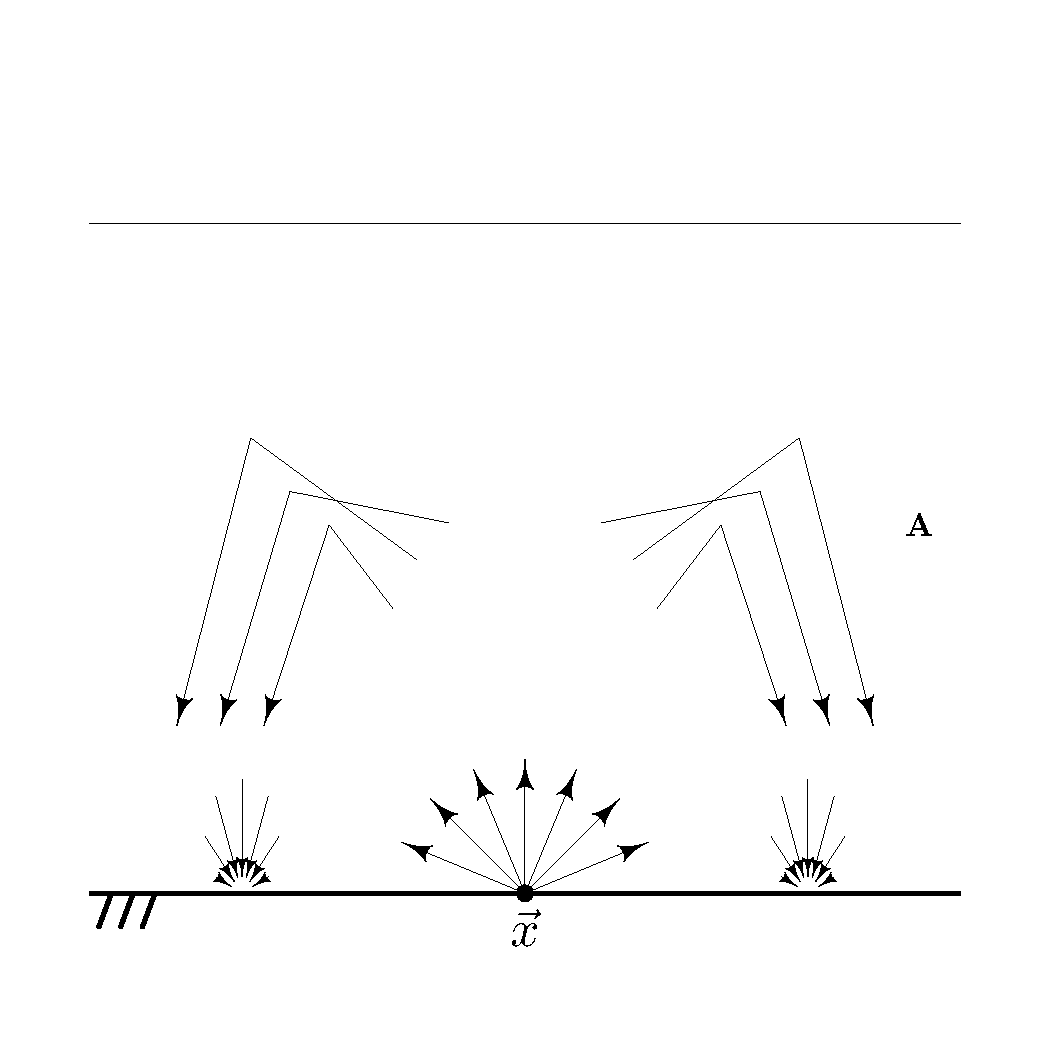
\includegraphics[trim=0 0 0 2cm, clip, width=0.45\linewidth]{sph_def}
  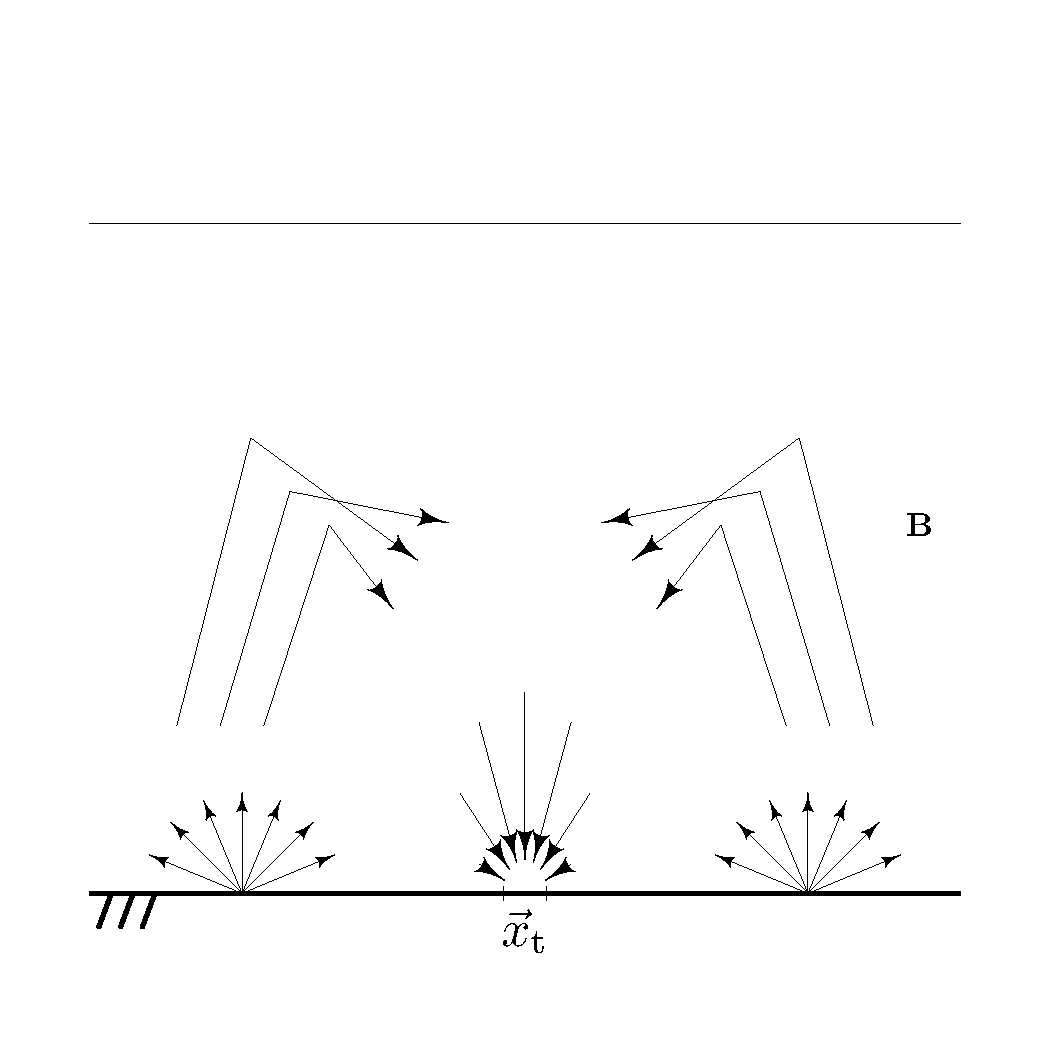
\includegraphics[trim=0 0 0 2cm, clip, width=0.45\linewidth]{sph_kernel}
  \caption{Illustration of the atmospheric spherical albedo. (A) The spherical albedo as the ratio of the integral over the surface of the plane irradiance received by each surface element to the irradiance emitted by the point isotropic source. (B) The spherical albedo as the ratio of plane irradiance received by a surface element to the integral of the irradiance emitted by an infinite number of isotropic point sources at the surface.}
  \label{fig:sph_albd_def}
\end{figure}

As described in Chapter~\ref{ch:theory}, the bi-hemispherical reflectance of the atmosphere when illuminated from below is the incident-average angular and spatial integral of the bidirectional scattering-surface reflectance distribution function (BSSRDF) of the atmosphere when illuminated by the surface, $\smash{\curlyvee_{\!\text{b}}(\hat{\xi}^\prime \rightarrow \hat{\xi}; \vec{x} - \vec{x}^{\, \prime})}$. Therefore, the spatially-resolved spherical albedo fuction (SAF), $\smash{\curlyvee_{\!\text{b}}(\hemiup \rightarrow \hemidn; \vec{x} - \vec{x}^{\, \prime})}$, is the incident-average angular integral of the BSSRDF. It is a spatial kernel that can be used for account the effects of an heterogeneous surface, as it maps the relative contribution of each surface element to the back-scattered downwelling plane irradiance received at the target surface element. The SAF kernel can be more intuitively linked to our application if we take the reciprocal definition of a plane irradiance received by a surface element when the surface plane has an infinite number of isotropic point sources. This definition is illustrated in Fig~\ref{fig:sph_albd_def}B.

Since in our definition the system has no other sources than the Sun, the illumination entering the atmosphere from below arises from surface reflection. Therefore, the specification of an isotropic source in the spherical albedo definition results that the BRDF of the surface must be given by the Lambert model. This is inline with the definitions in Chapter~\ref{ch:theory}. Though it ignores the variable BRDF of surface types, it should be noted that if the surface elements have arbitrary BRDFs and are randomly azimuthally oriented, the Lambert model is a reasonable assumption due to the spatial averaging over the surface contributing to the back-scattered energy at any given position. The implicit Lambertian BRDF results in a SAF that has a radial symmetry, independent of the surface bi-hemispherical reflectance magnitude and illumination conditions.

We can evaluate the SAF and the spherical albedo by simulation with a radiative transfer code \citep[\textit{cf.}][]{Leathers2004}. The radiative transfer calculations for RAdCor were carried out on a scalar backward Monte Carlo code specifically written for this project and available as a free and open source software (\textit{cf.} Appendix~\ref{ap:apsfs}). Fig.~\ref{fig:sph_albd_sim_kernel} shows two examples of SAF kernels for the 3rd waveband of the Operational Land Imager sensor on board Landsat 8. Figure~\ref{fig:sph_albd_sim_res} shows properties of the SAF for the different scatter types included in ACOLITE, while the magnitude and spectral dependency of the spherical albedo is shown in Fig.~\ref{fig:sph_albd_spectral}.

Further information is provided in Appendix~\ref{ap:apsfs} on how the spatially-resolved spherical albedo functions are calculated, fitted and reconstructed in RAdCor/ACOLITE for a specific combination of Rayleigh and aerosol contribution.

\begin{figure}[!htbp]
  \centering
  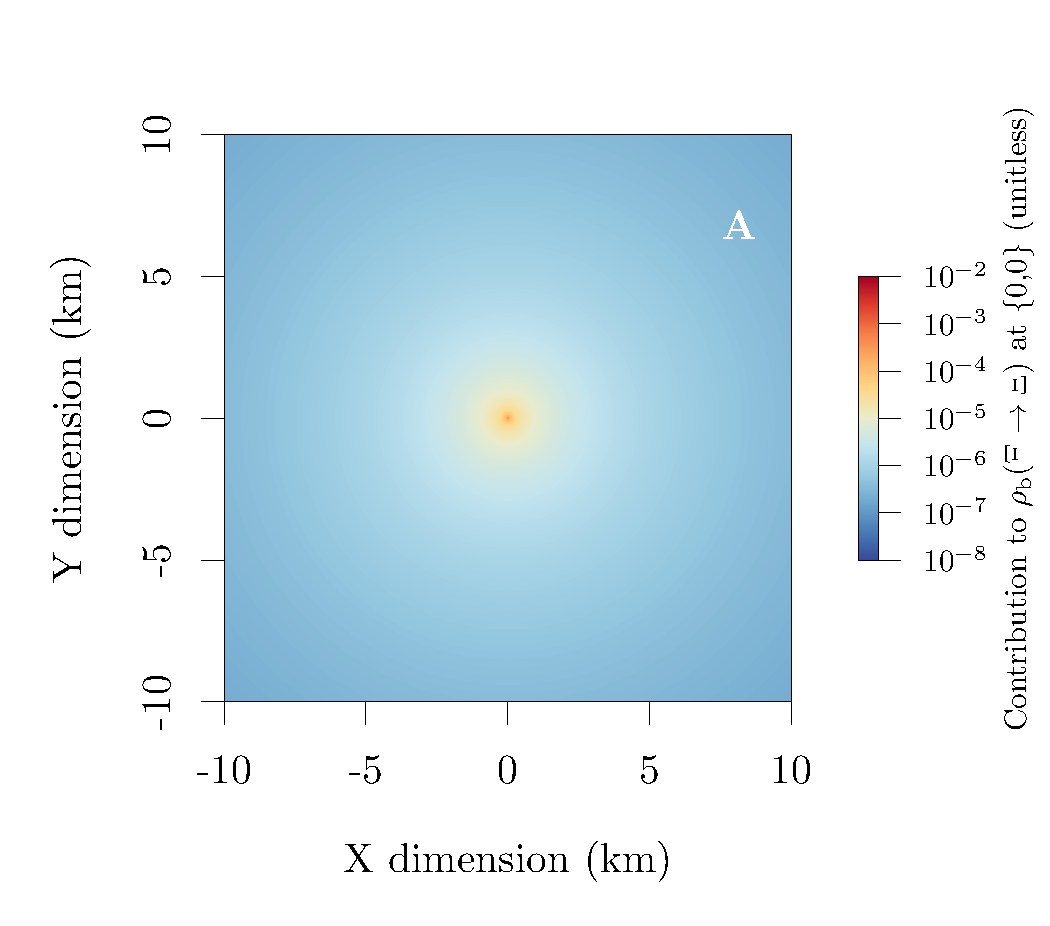
\includegraphics[width=0.45\linewidth]{saf_oli_r}
  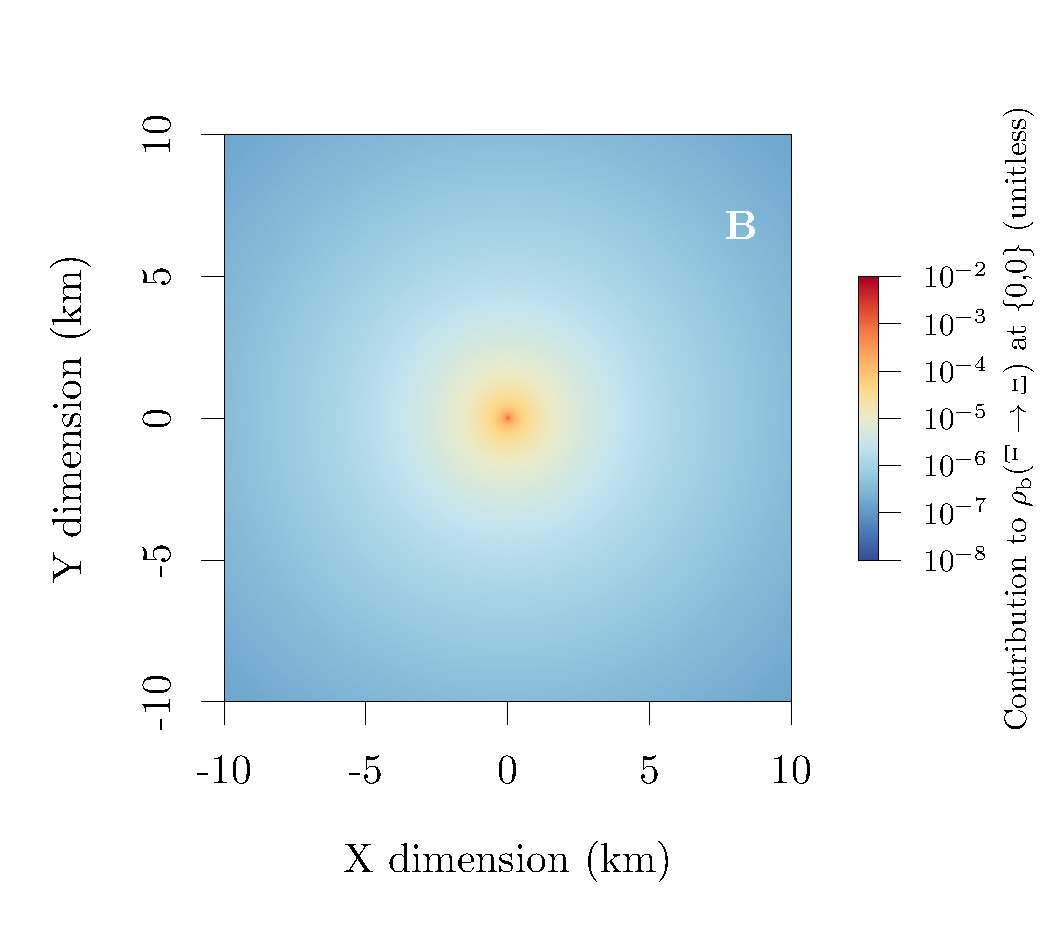
\includegraphics[width=0.45\linewidth]{saf_oli_c}
  \caption{SAF discrete kernels for the 3rd band of the Operational Land Imager on board Landsat~8. (A) Integro-normalised kernel for the Rayleigh scatter at standard atmospheric pressure (1013.25~mbar). (B) Integro-normalised kernel for a continental aerosol type at $\tau_\text{aer}(550)=0.5$ (unitless).}
  \label{fig:sph_albd_sim_kernel}
\end{figure}

\begin{figure}[!htbp]
  \centering
  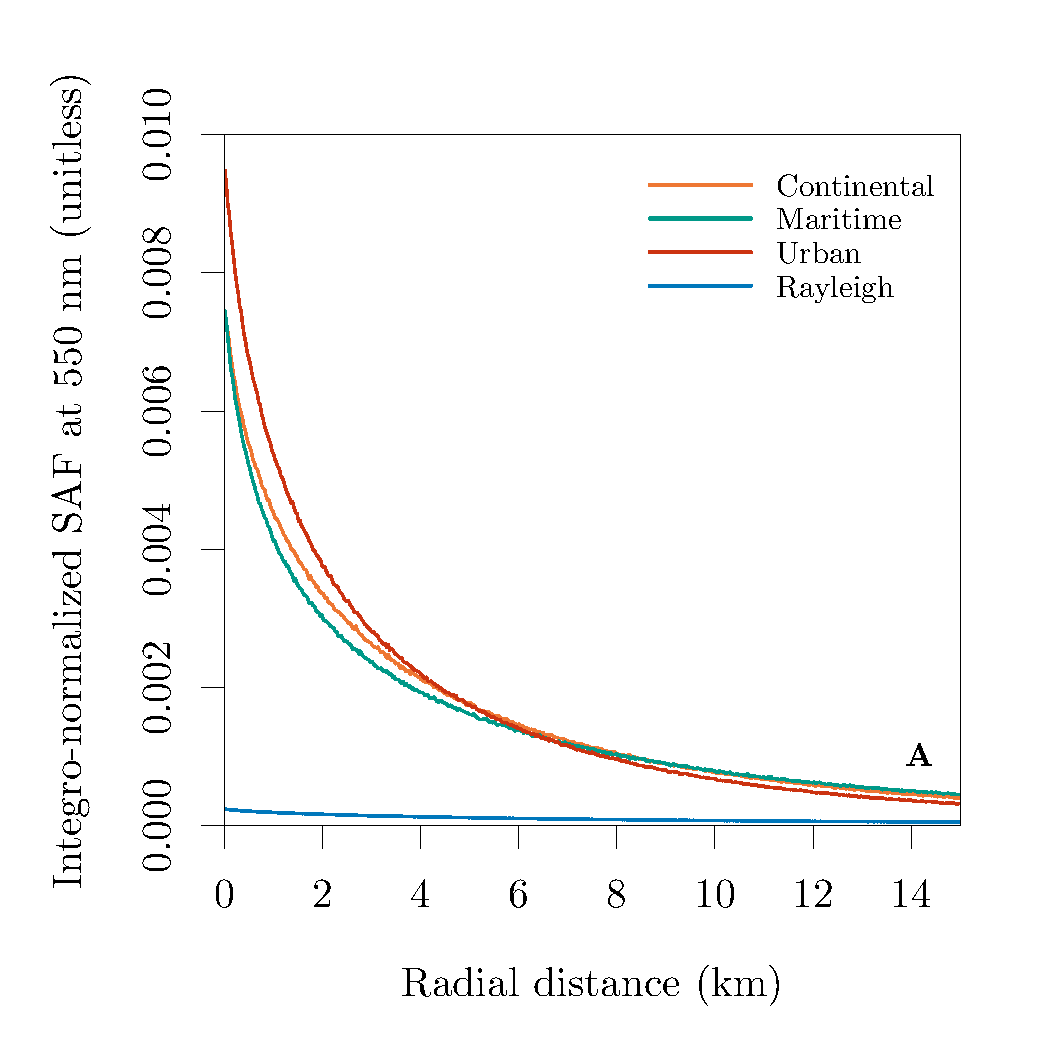
\includegraphics[width=0.45\linewidth]{saf_02_A}
  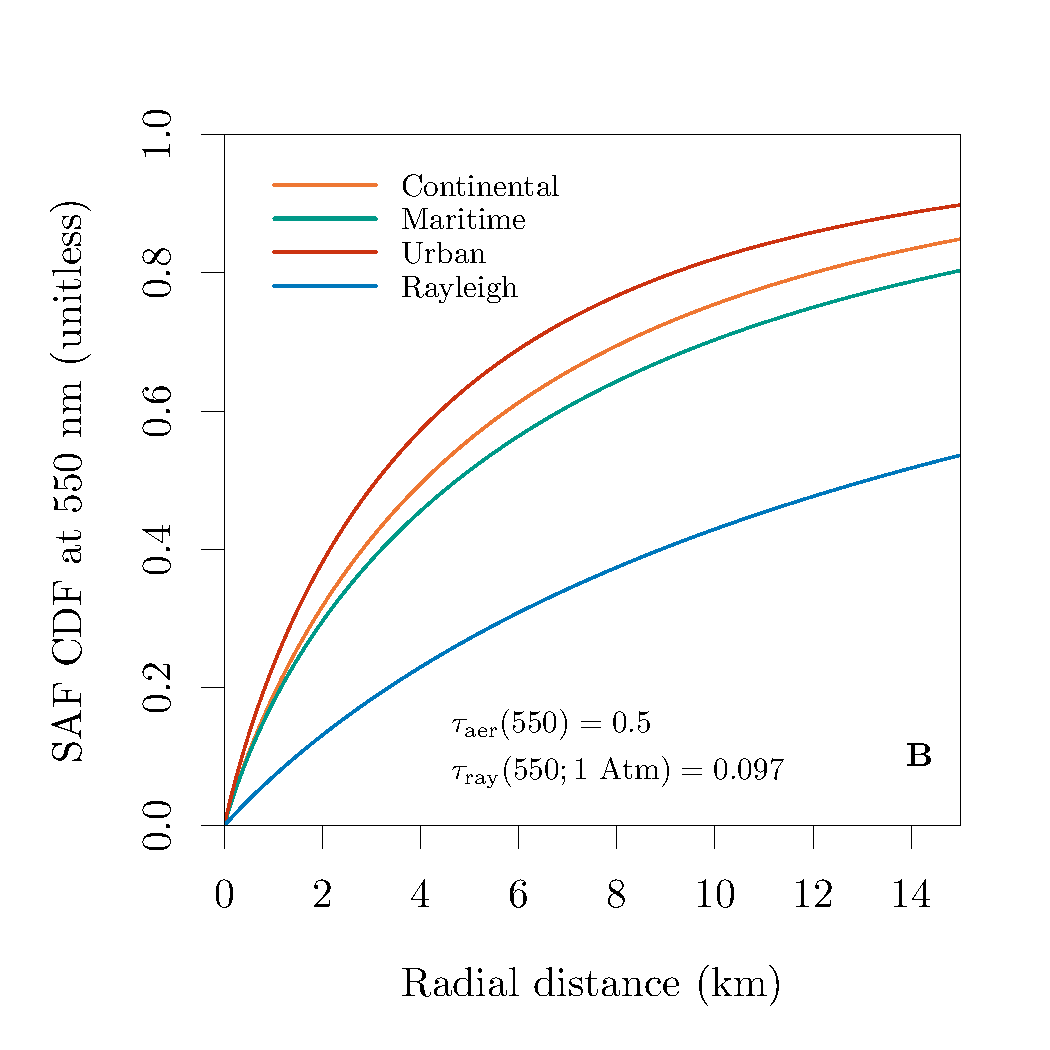
\includegraphics[width=0.45\linewidth]{saf_02_B}
  \caption{Annular integral of the integro-normalised spatially-resolved spherical albedo function (A) and its cumulative distribution function (B).}
  \label{fig:sph_albd_sim_res}
\end{figure}

\begin{figure}[!htbp]
  \centering
  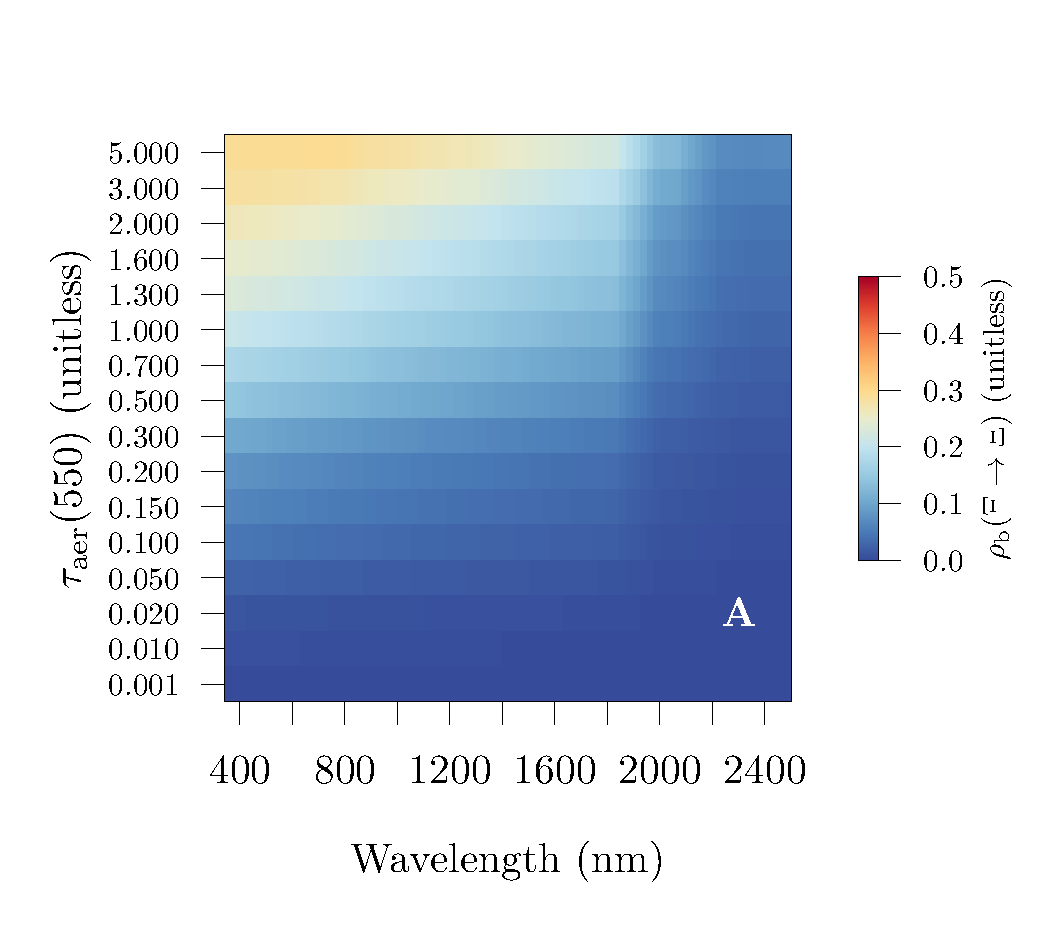
\includegraphics[trim=0.8cm 0.75cm 0.65cm 2.1cm, clip, width=0.45\linewidth]{s_spectral_a}
  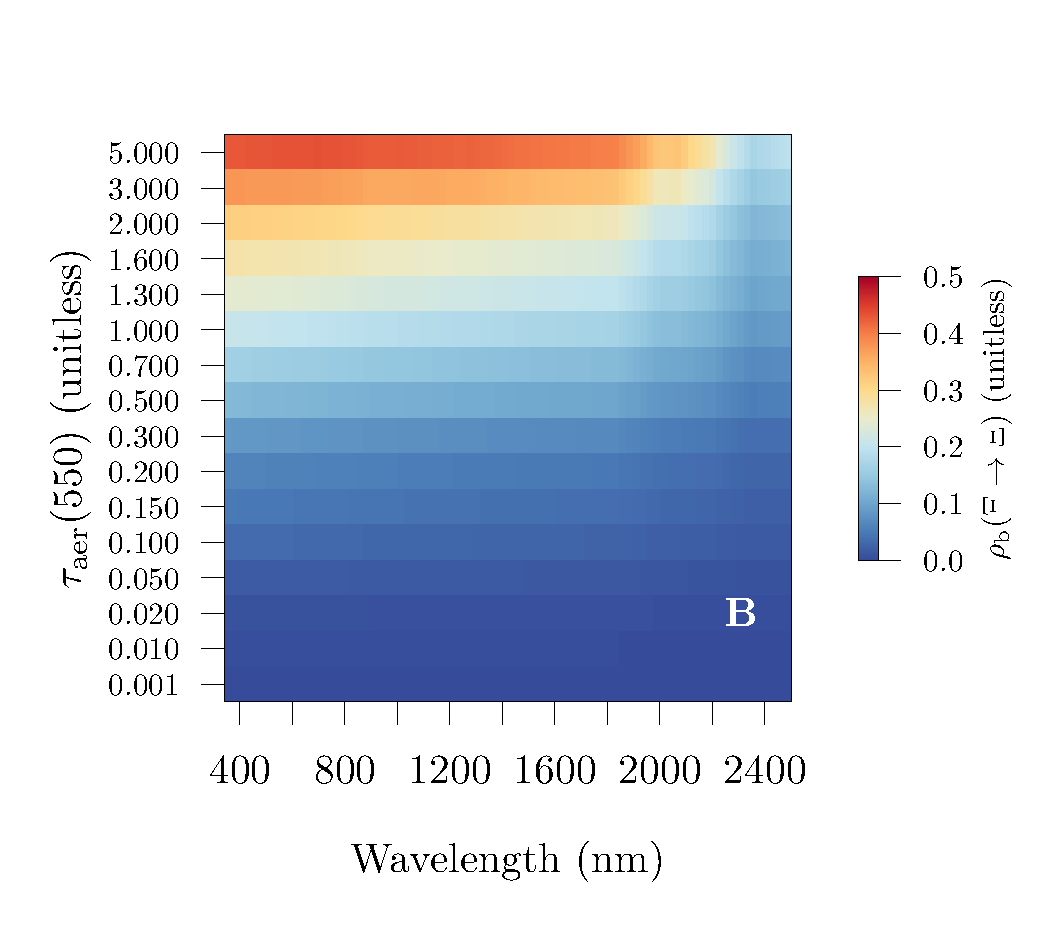
\includegraphics[trim=0.8cm 0.75cm 0.65cm 2.1cm, clip, width=0.45\linewidth]{s_spectral_b}
  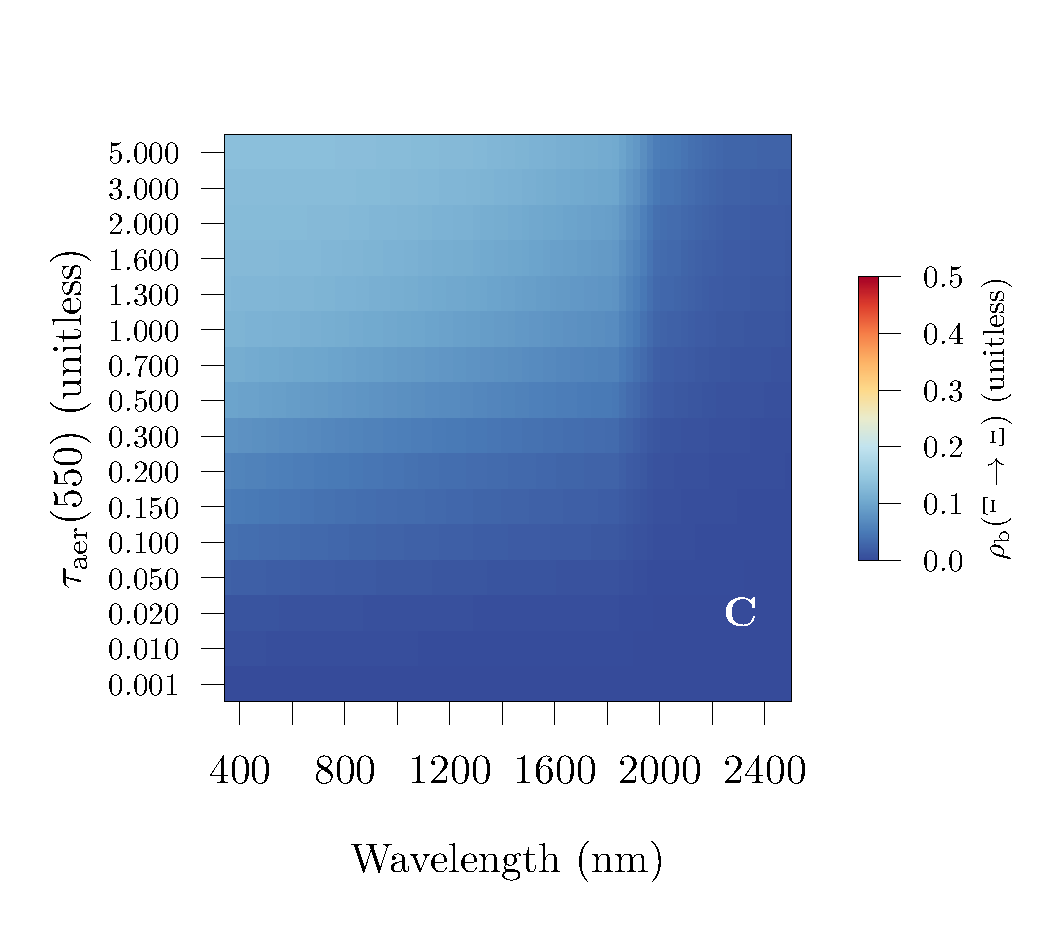
\includegraphics[trim=0.8cm 0.75cm 0.65cm 2.1cm, clip, width=0.45\linewidth]{s_spectral_c}
  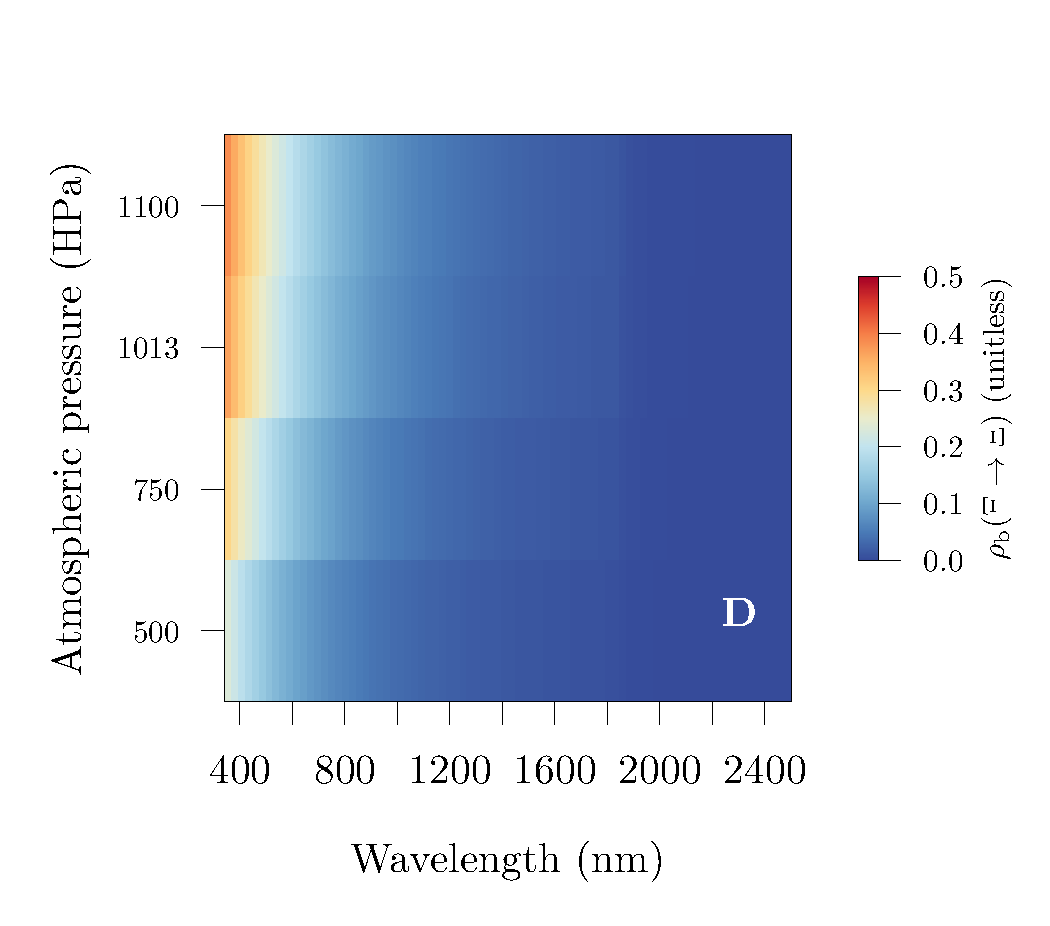
\includegraphics[trim=0.8cm 0.75cm 0.65cm 2.1cm, clip, width=0.45\linewidth]{s_spectral_d}
  \caption{The spherical albedo for the different scatter types included in ACOLITE. Continental (A), Maritime (B), and Urban (C) aerosols, as a function of the aerosol optical depth at~550 nm. (D) Rayleigh scatter, as a function of the atmospheric pressure at the surface.}
  \label{fig:sph_albd_spectral}
\end{figure}


\chapter{The atmospheric point spread function} \label{ch:psf}

The upward hemispherical-directional transmittance of the atmosphere, $T_{\text{u}_\text{tot}}(\hemiup \rightarrow \hat{\xi})$, can be defined as the ratio of the exitant radiance at top of the atmosphere (TOA) in a given direction to the incident irradiance from a isotropic point source located at the bottom of the atmosphere (BOA). It was shown in Chapter~\ref{ch:theory} that this transmittance is the incident-average spatial integral of the bidirectional scattering-surface transmission distribution function (BSSTDF) of the atmosphere when illuminated by the surface, $\smash{\curlywedge_{\!\text{b}}(\hat{\xi}^\prime \rightarrow \hat{\xi}; \vec{x} - \vec{x}^{\, \prime})}$. The intermediate function, retaining the spatial distribution of the emergent radiance transmitted to the sensor, $\smash{\curlywedge_{\!\text{b}}(\hemiup \rightarrow \hat{\xi}; \vec{x} - \vec{x}^{\, \prime})}$, is known as the atmospheric point spread function (PSF). These concepts are illustrated in Fig.~\ref{fig:atm_psf_def}A for nadir observation.

\begin{figure}[!htbp]
  \centering
  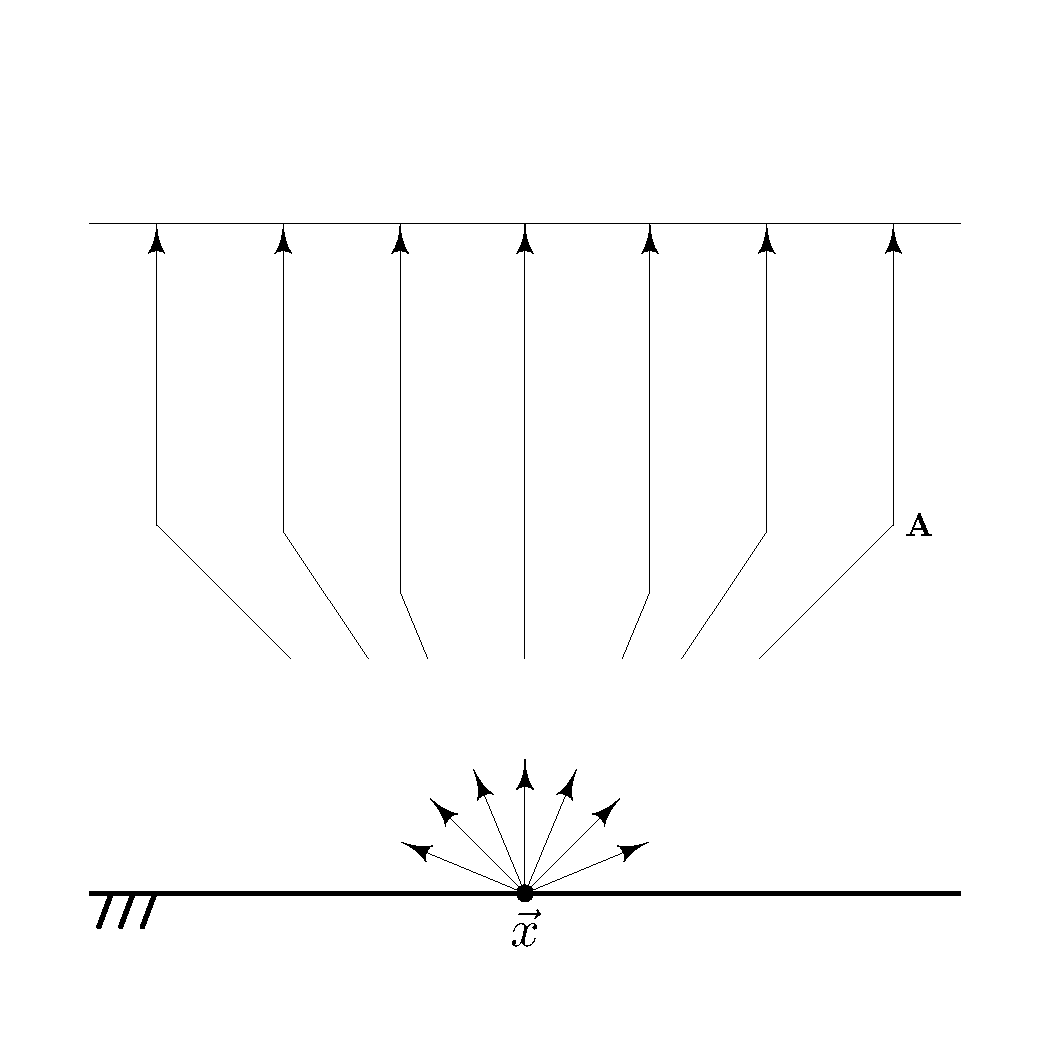
\includegraphics[trim=0 0 0 2cm, clip, width=0.45\linewidth]{psf_def}
  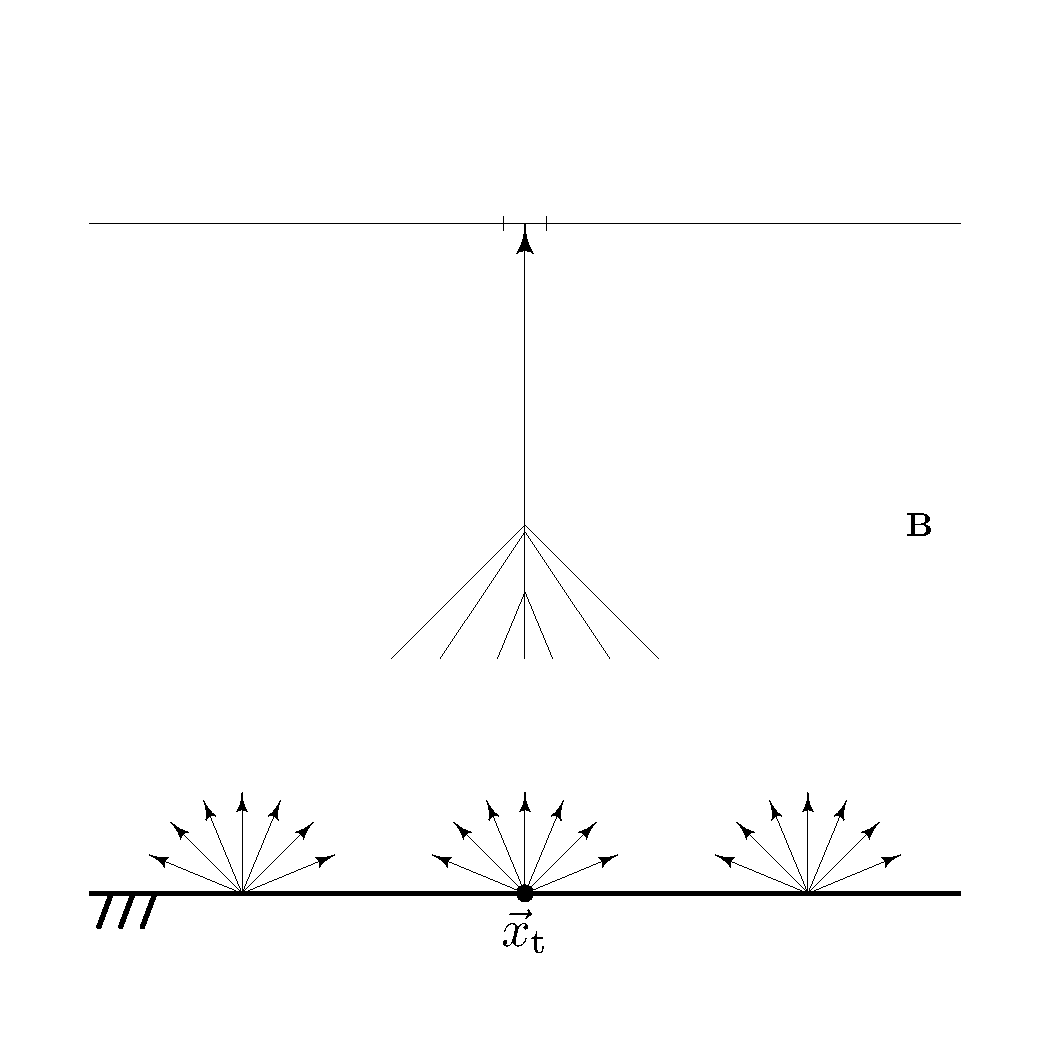
\includegraphics[trim=0 0 0 2cm, clip, width=0.45\linewidth]{psf_kernel}
  \caption{Illustration of the atmospheric point spread function (PSF). (A) The atmospheric PSF as the ratio of the radiance received at a given angle at the top of the atmosphere to the irradiance emitted by the point isotropic source. (B) The atmospheric PSF as the ratio of the radiance received at a given angle and position to the integral of the irradiance emitted by the an infinite number of isotropic point sources at the surface.}
  \label{fig:atm_psf_def}
\end{figure}

As for the spatially-resolved spherical albedo discussed in Chapter~\ref{ch:sph_albd}, the component with a spatial dimension in the definition can be swapped between receiving surface and source, to provide an equivalent definition of the PSF, but from the perspective of radiance incident at a single position and direction. This is illustrated in Fig.~\ref{fig:atm_psf_def}B for nadir observation. This perspective more intuitively relates to the spatial kernel mapping the contribution of the each surface element to the transmitted radiance at TOA, received by a single detector element oriented in a given view direction. Once more, the use of isotropic point sources implies, for reflection, a Lambertian BRDF of the surface, which is in line with the system definitions in Chapter~\ref{ch:theory}.

The atmospheric PSF includes the direct and diffuse transmission. The direct transmittance can be easily calculated from the attenuation law (Eq.~\ref{eq:theory_tdir}) for a given atmosphere composition and pathlength. It can be represented in the BSSTDF formalism by resorting to Dirac delta functions (Eq.~\ref{eq:theory_tudir_pulse_d}). The resulting pulse function transmits only the radiance at the origin, $\smash{\vec{x} - \vec{x}^{\, \prime} = \vec{0}}$. A schematic representation of the direct and diffuse kernels of the atmospheric PSF is presented in Fig.~\ref{fig:psf_scheme_components}.

\begin{figure}[!htbp]
  \centering
  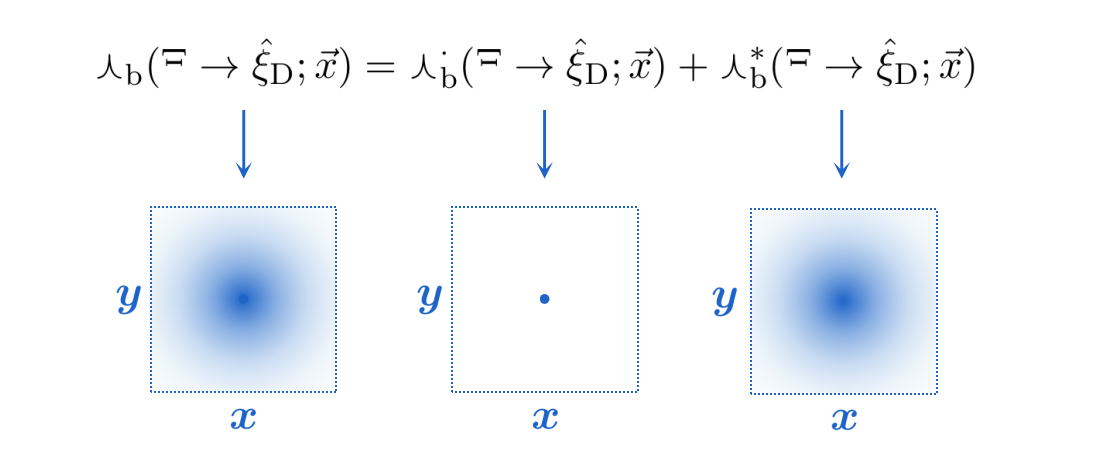
\includegraphics[width=0.6\linewidth]{psf_scheme_components.png}
  \caption{Schematic representation of the atmospheric PSF kernel components, as given by Eq.~\ref{eq:theory_psf_tot}.}
  \label{fig:psf_scheme_components}
\end{figure}

The diffuse component involves multiple scatter and requires the use of a radiative transfer code. The radiative transfer code written for RAdCor (\textit{cf.} Appendix~\ref{ap:apsfs}) was used to create a look-up-table of pre-calculated atmospheric diffuse PSFs for the scatter types included in ACOLITE. Figure~\ref{fig:psf_sim_res} shows properties of the diffuse PSF for those scatter types. Examples of the integro-normalised atmospheric diffuse PSF kernel are presented in Fig.~\ref{fig:psf_sim_kernel}. The magnitude and spectral dependency of diffuse fraction of the total upward diffuse transmission is presented in Fig.~\ref{fig:psf_diffrat_spectral}.

Further information is provided in Appendix~\ref{ap:apsfs} on how the atmospheric diffuse point spread functions are calculated, fitted and reconstructed in RAdCor/ACOLITE for a specific combination of Rayleigh and aerosol contribution.

\begin{figure}[!htbp]
  \centering
  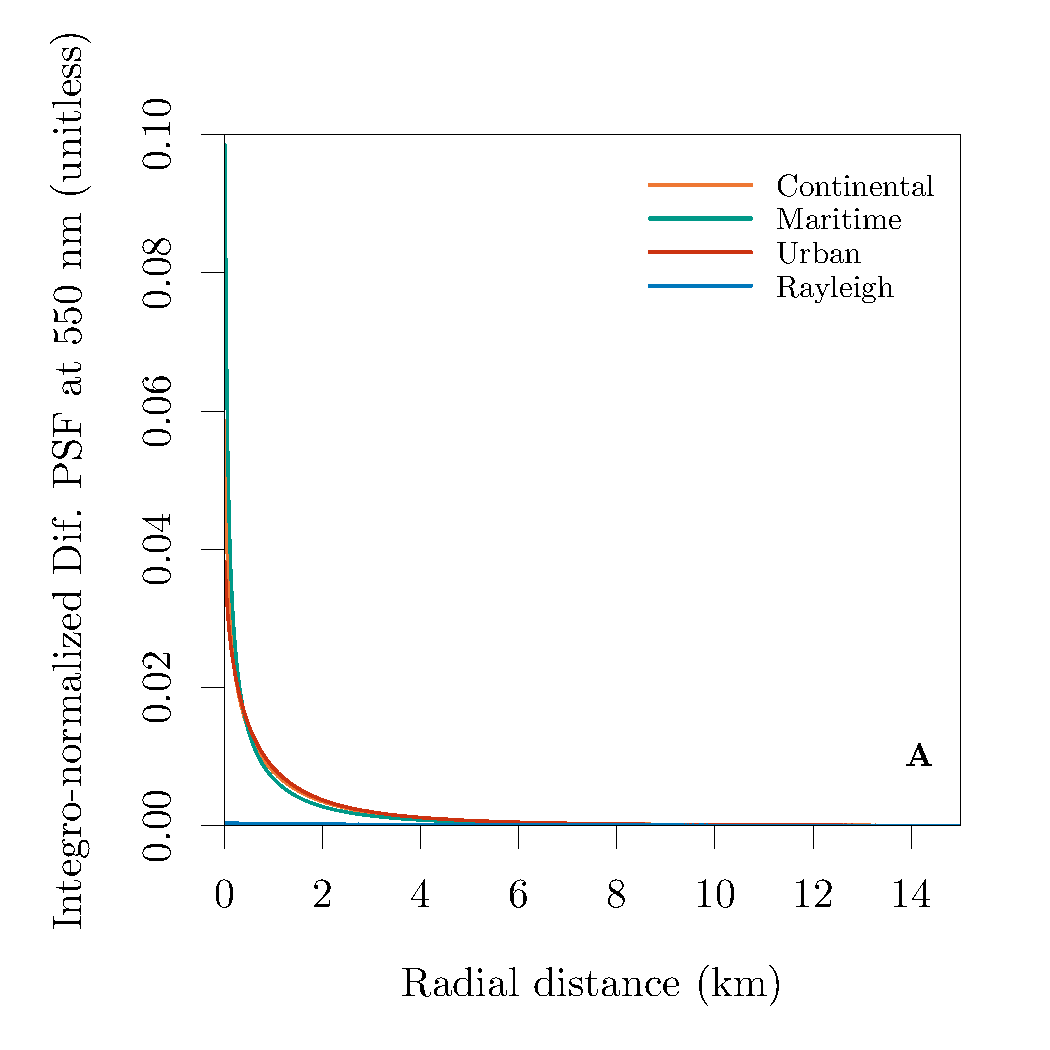
\includegraphics[width=0.45\linewidth]{psf_sim_A}
  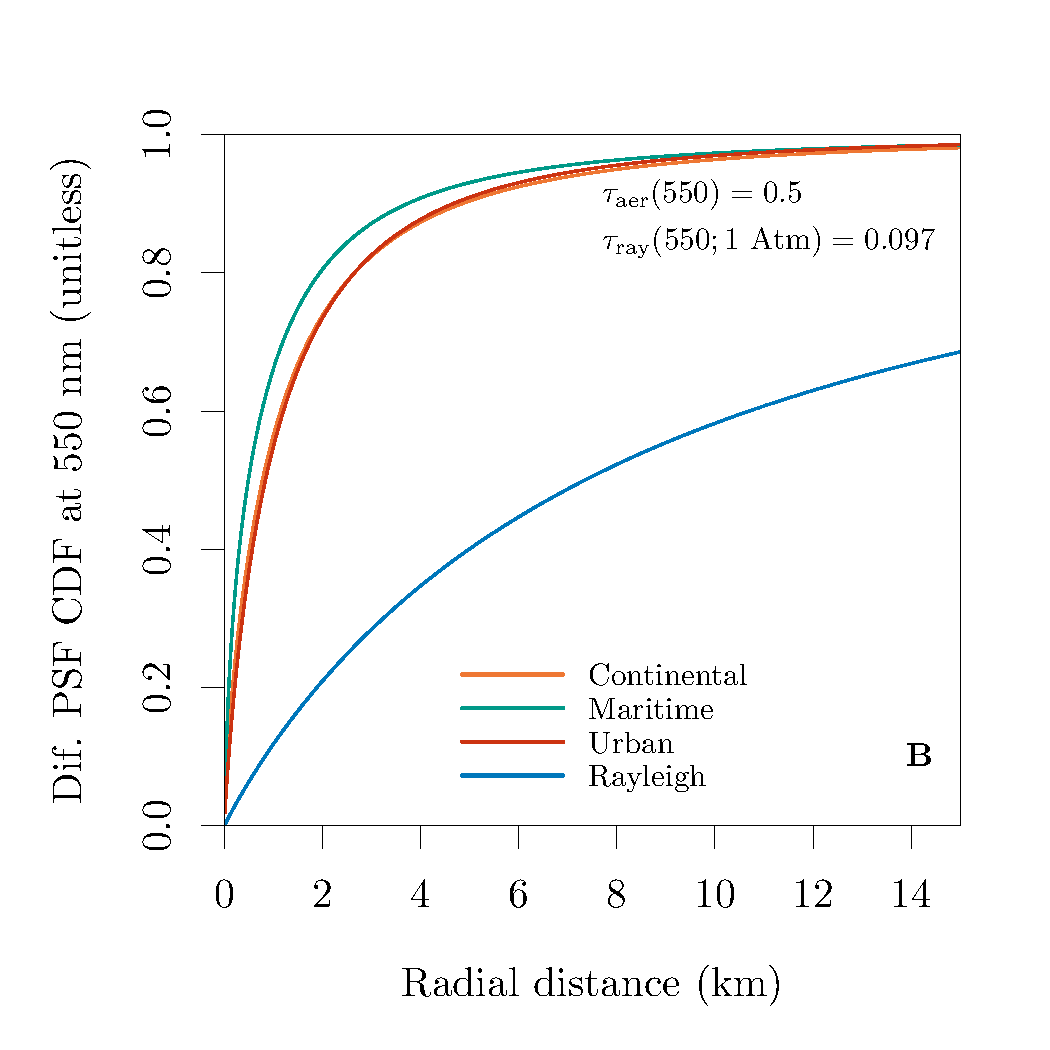
\includegraphics[width=0.45\linewidth]{psf_sim_B}
  \caption{Integro-normalised atmospheric diffuse point spread function (A) and its cumulative distribution function (B).}
  \label{fig:psf_sim_res}
\end{figure}

\begin{figure}[!htbp]
  \centering
  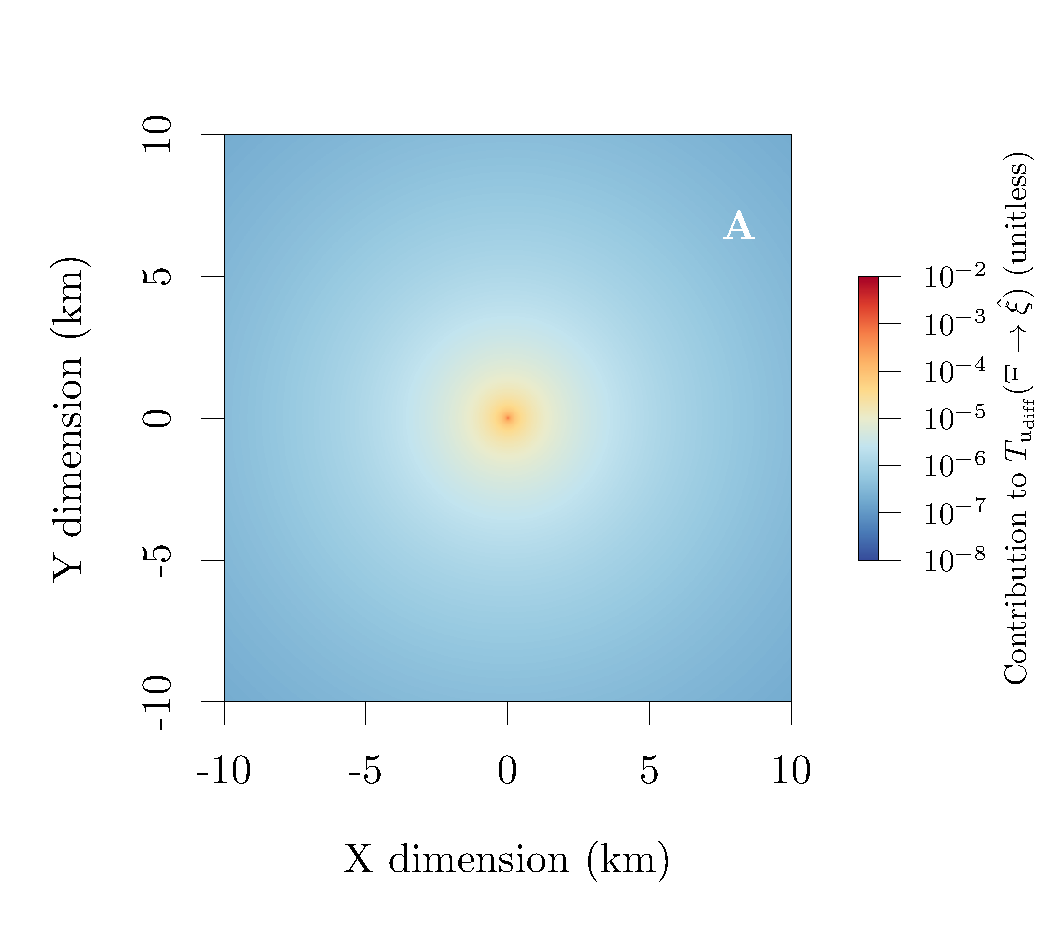
\includegraphics[width=0.45\linewidth]{psf_oli_00_r}
  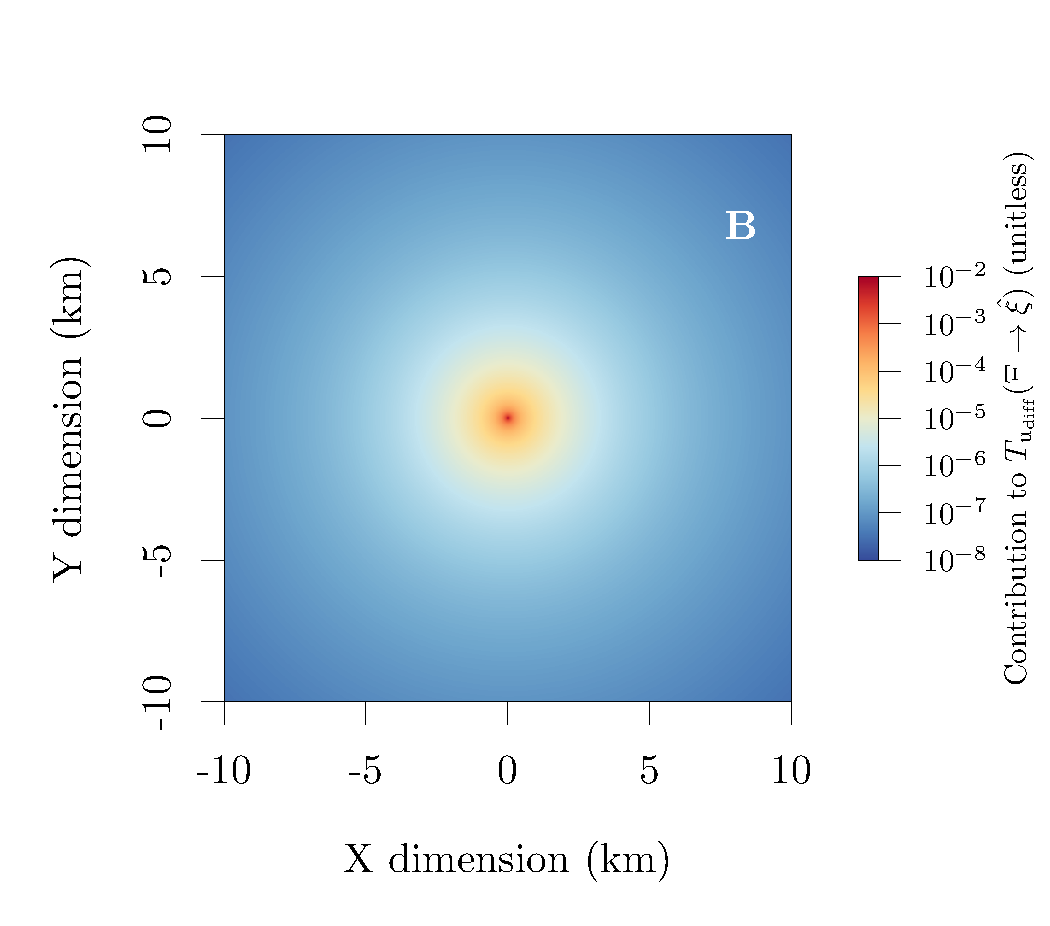
\includegraphics[width=0.45\linewidth]{psf_oli_00_c}
  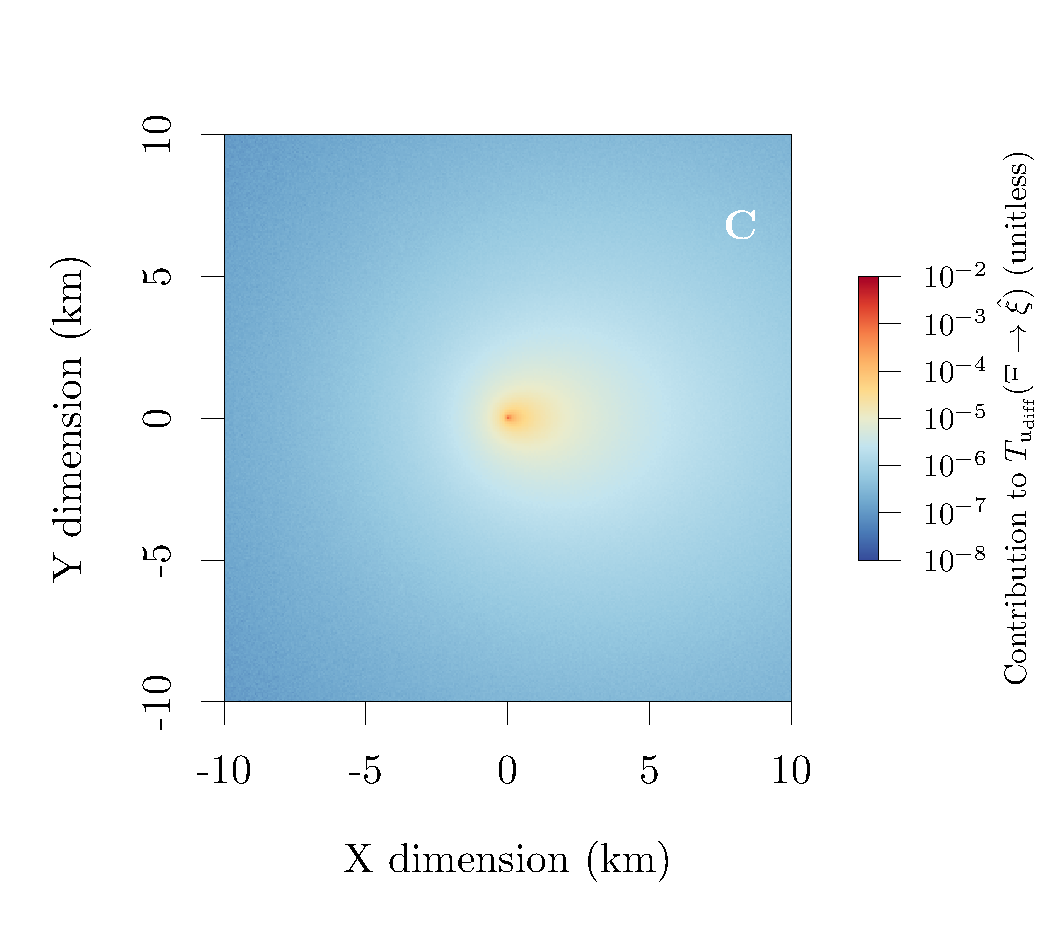
\includegraphics[width=0.45\linewidth]{psf_oli_40_r}
  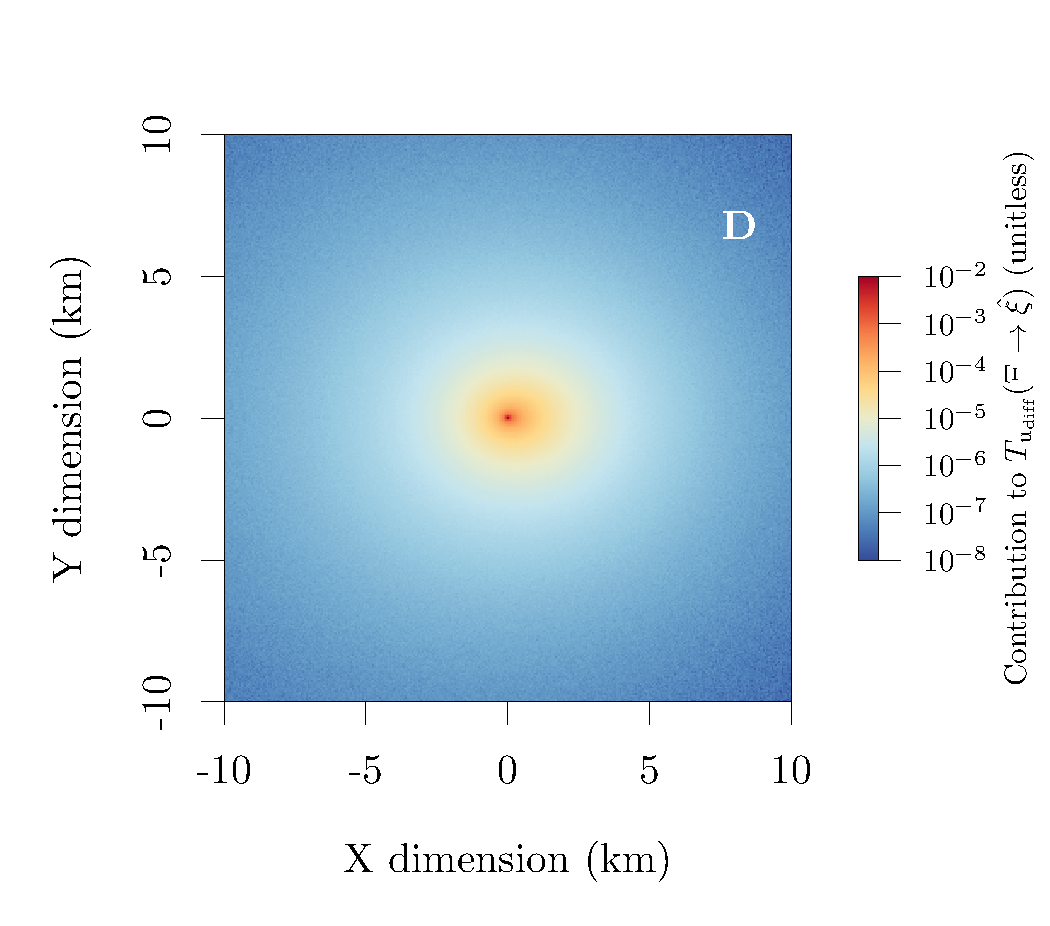
\includegraphics[width=0.45\linewidth]{psf_oli_40_c}
  \caption{Atmospheric diffuse PSF discrete kernels for the 3rd band of the Operational Land Imager on board Landsat~8. (A) Integro-normalised kernel for the Rayleigh scatter and nadir observation. (B) Integro-normalised kernel for a continental aerosol type and nadir observation. (C) and (D) the same as (A) and (B) but for a 40$^{\circ}$ view zenith angle (270$^{\circ}$ view azimuth angle).}
  \label{fig:psf_sim_kernel}
\end{figure}

\begin{figure}[!htbp]
  \centering
  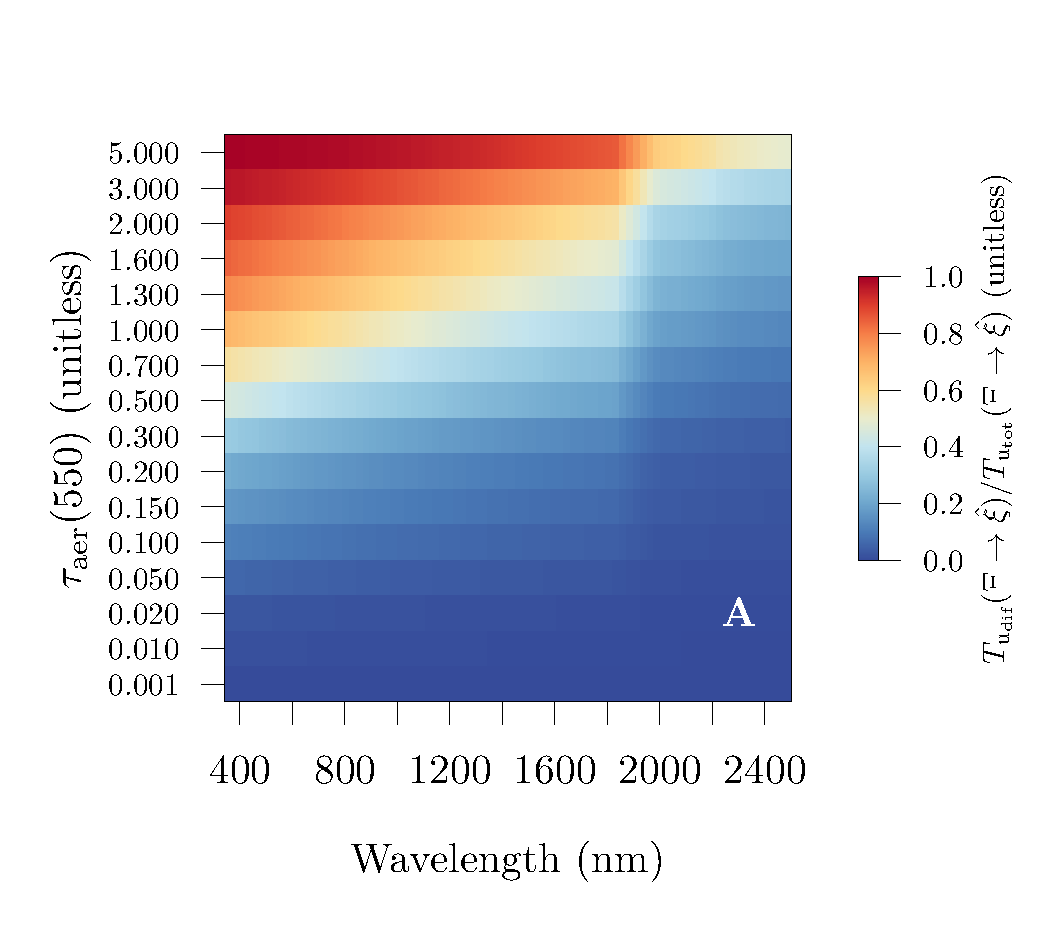
\includegraphics[trim=0.8cm 0.75cm 0.65cm 2.1cm, clip, width=0.45\linewidth]{ut_spectral_a}
  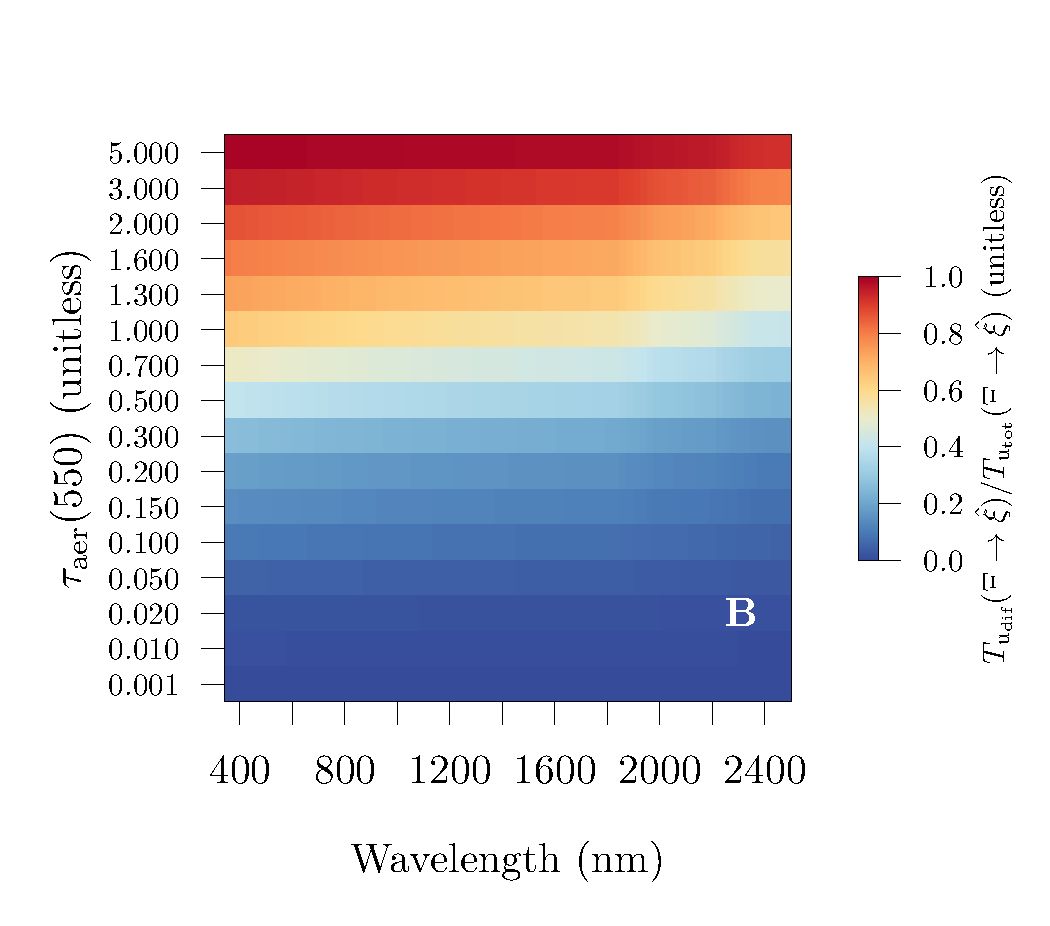
\includegraphics[trim=0.8cm 0.75cm 0.65cm 2.1cm, clip, width=0.45\linewidth]{ut_spectral_b}
  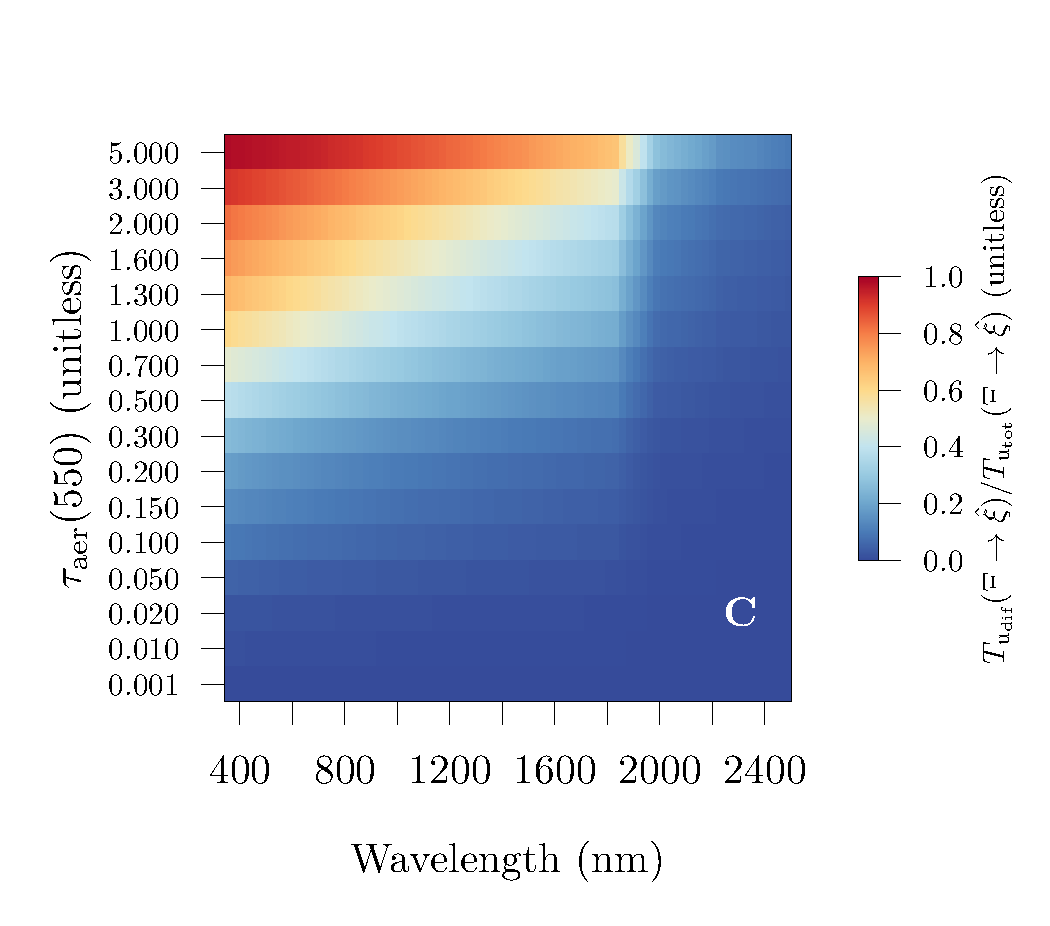
\includegraphics[trim=0.8cm 0.75cm 0.65cm 2.1cm, clip, width=0.45\linewidth]{ut_spectral_c}
  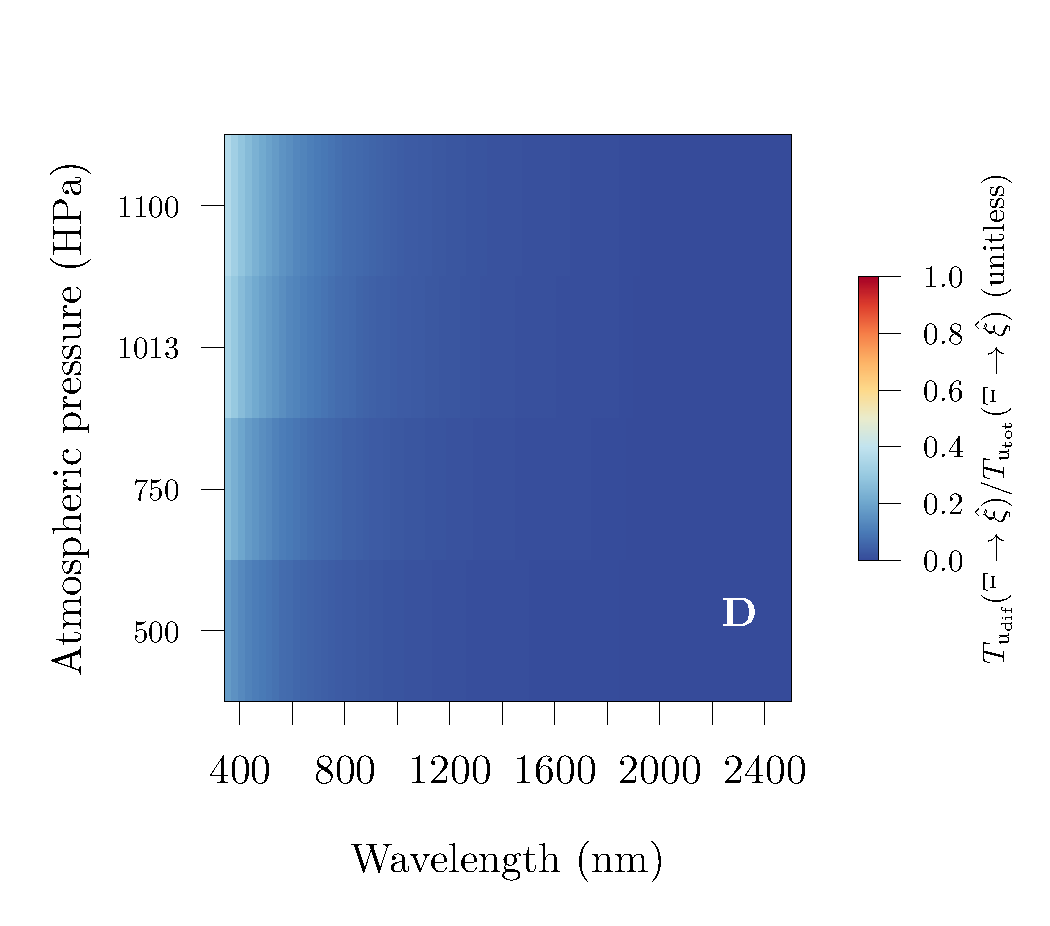
\includegraphics[trim=0.8cm 0.75cm 0.65cm 2.1cm, clip, width=0.45\linewidth]{ut_spectral_d}
  \caption{The fraction of $T_{\text{u}_\text{dif}}(\hemiup \rightarrow \hat{\xi})$ from $T_{\text{u}_\text{tot}}(\hemiup \rightarrow \hat{\xi})$ for the different scatter types included in ACOLITE. Continental (A), Maritime (B), and Urban (C) aerosols, as a function of the aerosol optical depth at 550 nm. (D) Rayleigh scatter, as a function of the atmospheric pressure at the surface.}
  \label{fig:psf_diffrat_spectral}
\end{figure}


\chapter{Estimation of atmospheric optical properties} \label{ch:ts_dsf}

The optical depth due to gaseous scattering \citep{Bodhaine1999} can be well approximated from standard atmosphere models \citep[\textit{e.g.},][]{US1976} modified by the atmospheric pressure at the surface. The atmospheric pressure at the surface itself is available daily and in global coverage from meteorological data assimilation and models \citep[\textit{e.g.}][]{Kanamitsu2002}, or can be well approximated by local altitude available from global coverage surface elevation models \citep[\textit{e.g.}][]{Airbus2022}. Additionally, external information is typically available daily and in global coverage about the concentration of absorbing gases from suits of Earth observation missions designed for atmospheric observation. Scattering due to turbulent flow (\textit{e.g.}, convection due to surface heating) is a minor effect for vertical observations through the atmosphere and is typically neglected. Therefore, the crucial component is the estimation of the aerosol optical properties, which depends on the aerosol model (composition and size distribution) and vertical profile, with the later typically taken as a standard profile \citep[\textit{e.g.},][]{Hess1998}.

The atmosphere's bidirectional reflectance when illuminated from above, $\smash{\rho_\text{a}(\hat{\xi}_0 \rightarrow \hat{\xi}_\text{D})}$, presented as component \textbf{I} in Fig.~\ref{fig:theory_components_A} is the basis for estimating aerosol properties from remote observations when external information about the aerosols is not available. It corresponds to the signal that would be observed if the entire surface $S$ was non-reflective at the wavelength of observation or at wavelengths of large atmosphere optical thickness with low single scattering albedo, in which case the signal from the surface is not transmitted to the sensor. For those reasons, this component cannot be directly observed in wavelength ranges of interest for surface observation, but it can be approximated by the signal recorded over surfaces of low reflectance over a large spatial scale. An example of such a condition are observations over the open ocean in the near-infrared (NIR), which is well approximated by the homogeneous surface framework due to the low contrast between adjacent surface areas. Alternatively, $\smash{\rho_\text{a}(\hat{\xi}_0 \rightarrow \hat{\xi}_\text{D})}$ can be approximated by the signal recorded over patches of surfaces of low reflectance under relatively low atmospheric scattering, as the recorded signal will include only small amounts of signal from the surrounding surfaces \citep[\textit{e.g.} in the shortwave-infrared, SWIR, for low to moderate aerosol concentration;][]{Fraser1964}. In the later, while the surface system does not conform to the homogeneous surface framework, the upward diffuse transmittance of the atmosphere is small such that the homogeneous surface framework applies locally over the low reflective patch. For turbid atmospheres over patchy surfaces, however, the contribution of the diffusely transmitted signal from surrounding surfaces to the signal recorded over the low reflective patch can result in a poor approximation to $\smash{\rho_\text{a}(\hat{\xi}_0 \rightarrow \hat{\xi}_\text{D})}$.

In this chapter we will provide an overview of two well known approaches for estimation of aerosol composition and concentration developed under the homogeneous surface reflectance framework and develop a more general method for estimation of those properties that can be applied over heterogeneous surfaces. In the development of the equations of this chapter, we will consider that the scene extent is large enough around the region of interest to contain the full area contributing to the diffusely transmitted signal from the surface to the sensor for the region of interest. The consequences and adaptations necessary to handle spatially finite kernels and scenes will be developed in Chapter~\ref{ch:finite}.

% Section -------------------------------------------------------------------
\section{Aerosol estimation over homogeneous surfaces}

One commonly used approach for estimation of aerosol properties is known as the ``black pixel'' approach\endnotemark{}, developed for estimation of aerosol properties over open ocean scenes \citep{Gordon1994}. Pure (sea)water has a high absorption coefficient in the NIR and SWIR, while open ocean waters are typically characterised by low concentration of hydrosols, resulting that for observations avoiding the sun glint, the water system reflectance from the NIR to SWIR is negligible when compared to $\smash{\rho_\text{a}(\hat{\xi}_0 \rightarrow \hat{\xi}_\text{D})}$. This can be represented as:

\endnotetext{The term ``black pixel'' is somewhat a misnomer for this approach, as the pixel is assumed to be non-reflective only at some wavebands. The term ``NIR-SWIR black pixel'' would better describe the approach.}

\begin{equation}
\frac{\rho_\text{as}(\hat{\xi}_0 \rightarrow \hat{\xi}_\text{D}; \Lambda_w; \vec{x})}{T_\text{g}(\hat{\xi}_0; \hat{\xi}_\text{D}; \Lambda_w)} =  \rho_\text{a}(\hat{\xi}_0 \rightarrow \hat{\xi}_\text{D}; \Lambda_w; \vec{x}) + \varepsilon(\Lambda_w),
\label{eq:ts_dsf_rhoa}
\end{equation}

\noindent where $\smash{\Lambda_w}$ is the normalised spectral response function (SRF) of waveband $w$, $\smash{T_\text{g}(\hat{\xi}_0; \hat{\xi}_\text{D}; \Lambda_w)}$, unitless, is the transmittance due to gaseous absorption for the illumination-observation geometry, and $\smash{\varepsilon(\Lambda_w)}$ is the residual signal from the surface, typically on the order of $\approx 1~\%$ of $\smash{\rho_\text{a}(\hat{\xi}_0 \rightarrow \hat{\xi}_\text{D}; \Lambda_w)}$ and can be neglected. This signal can be compared against simulations of $\smash{\rho_\text{a}(\hat{\xi}_0 \rightarrow \hat{\xi}_\text{D}; \Lambda_w)}$ for atmospheres with different aerosol compositions and concentrations, given by the aerosol optical thickness, $\smash{\tau_\text{aer}(\Lambda_w)}$. The spectra, in case more than one waveband is available where the surface can be considered ``dark'', is used to select the aerosol model that provides the best fit to the spectral observation, when considering the external inputs of atmospheric pressure at the surface, absorbing gases concentration and illumination-observation geometry. The selection of aerosol model is essential to estimate the aerosol optical effects in other wavebands in which the surface signal cannot be considered negligible. Because the spectral shape of the aerosol optical thickness is defined by the aerosol model, it is typical to specify the aerosol optical thickness at a single wavelength, commonly at 550 nm, $\smash{\tau_\text{aer}(550)}$. This ``black pixel'' approach is typically applied per pixel, allowing the atmosphere composition to vary between neighbouring pixels, thus $\smash{\rho_\text{a}(\hat{\xi}_0 \rightarrow \hat{\xi}_\text{D}; \Lambda_w; \vec{x})}$ retaining the spatial dependency in Eq.~\ref{eq:ts_dsf_rhoa}.

When every pixel for an arbitrary scene cannot be expected to be ``black'' in any of the wavebands available for the sensor, an alternative to the ``black pixel'' is the ``Dark Spectrum Fitting'' approach \citep{Vanhellemont2018}. This method was developed in the context of high spatial resolution sensors, that could resolve shadows of structures in the scene, extrapolating the aerosol parameters estimated over the dark patch to a larger spatial extent. In this method, the pixels with the lowest $\smash{\rho_\text{as}(\hat{\xi}_0 \rightarrow \hat{\xi}_\text{D}; \Lambda_w; \vec{x})}$ in each waveband are selected to build a ``dark spectrum'' at TOA, $\smash{\rho_\text{as}^\text{TDark}(\hat{\xi}_0 \rightarrow \hat{\xi}_\text{D}; \Lambda_w)}$. The dark spectrum is interpreted with Eq.~\ref{eq:ts_dsf_rhoa}, resulting in one estimation of $\smash{\tau_\text{aer}(550)}$ per waveband and per aerosol model, with the selection of the lowest $\smash{\tau_\text{aer}(550)}$ for each aerosol model. The selection of the lowest $\smash{\tau_\text{aer}(550)}$ for a given aerosol model ensures a lower bound fit of $\smash{\rho_\text{a}(\hat{\xi}_0 \rightarrow \hat{\xi}_\text{D}; \Lambda_w)}$ to $\smash{\rho_\text{as}^\text{TDark}(\hat{\xi}_0 \rightarrow \hat{\xi}_\text{D}; \Lambda_w)}$, that is, it ensures that surface reflectances are non-negative. The aerosol model is selected as before, based on the best lower bound fit between $\smash{\rho_\text{a}(\hat{\xi}_0 \rightarrow \hat{\xi}_\text{D}; \Lambda_w)}$ to $\smash{\rho_\text{as}^\text{TDark}(\hat{\xi}_0 \rightarrow \hat{\xi}_\text{D}; \Lambda_w)}$ over all aerosol models. This approach is typically applied per scene or per spatial subsets of the scene (\textit{e.g.} 7~km $\times$ 7~km), also called ``tiles'', over which the atmosphere is assumed to have the same composition, thus the spatial dependency is dropped from $\smash{\rho_\text{a}(\hat{\xi}_0 \rightarrow \hat{\xi}_\text{D}; \Lambda_w)}$ in Eq.~\ref{eq:ts_dsf_rhoa}.

While the DSF approach, under the assumption of homogeneity of the atmosphere over a given spatial scale, in essence generalises the ``black pixel'' approach by not prescribing the wavebands with near-zero surface reflectance, it is still limited to situations of low atmospheric turbidity. When the upward diffuse transmittance increases, the darkest pixel at TOA might not be the darkest pixel at the surface, depending on the reflectance contrast and spatial dimensions of near-by surfaces. Even for scenes where the darkest pixel at TOA and at the surface are equivalent, $\smash{\varepsilon(\Lambda_w)}$ might be non-negligible due to the adjacency signal from surrounding bright surfaces. In other words, the method of selection of reference pixels in DSF does not consider the impact of surrounding surfaces and the interpretation of the signal over the reference pixels does not consider the effect of atmospheric blurring.

% Section -------------------------------------------------------------------
\section{Aerosol estimation over heterogeneous surfaces}

In RAdCor we further generalise the DSF method from a homogeneous surface framework to a heterogeneous surface framework. We do this by estimating $\smash{\tau_\text{aer}(550)}$ not from $\smash{\rho_\text{as}^\text{TDark}(\hat{\xi}_0 \rightarrow \hat{\xi}_\text{D}; \Lambda_w)}$ but from the TOA signal of the darkest pixels at the surface, $\smash{\rho_\text{as}^{\text{SDark}}(\hat{\xi}_0 \rightarrow \hat{\xi}_\text{D}; \Lambda_w)}$. As discussed before, the darkest pixel at the surface might not be the darkest pixel at TOA due to the diffuse transmittance of the spatially variable reflectance of the surrounding pixels. We attempt to find the darkest pixels at the surface by introducing an hypothetical quantity, $\smash{\rho_\text{as}^\text{Hyp}(\hat{\xi}_0 \rightarrow \hat{\xi}_\text{D}; \Lambda_w; \vec{x})}$. This quantity is the apparent surface reflectance at TOA that would be observed if all upward transmittance was diffuse. It is defined based on Eq.~\ref{eq:theory_me_closed_form} as:

\begin{equation}
\openup 2\jot
\begin{split}
&\frac{\rho_\text{as}^\text{Hyp}(\hat{\xi}_0 \rightarrow \hat{\xi}_\text{D}; \Lambda_w; \vec{x})}{T_\text{g}(\hat{\xi}_0; \hat{\xi}_\text{D}; \Lambda_w)} = \\ 
& \rho_\text{a}(\hat{\xi}_0 \rightarrow \hat{\xi}_\text{D}; \Lambda_w) + T_{\text{d}_\text{tot}}(\hat{\xi}_0 \rightarrow \hemidn; \Lambda_w) \, \rho_{\text{s}_{\!\curlywedge_\text{b}^*}}(\hemidn \rightarrow \hemiup; \Lambda_w; \vec{x}) \, T_{\text{u}_\text{tot}}(\hemiup \rightarrow \hat{\xi}_\text{D}; \Lambda_w),
\end{split}
\label{eq:ret_rho_env_toa}
\end{equation} 
\begin{equation}
\openup 2\jot
\begin{split}
\rho_{\text{s}_{\!\curlywedge_\text{b}^*}}&(\hemidn \rightarrow \hemiup; \Lambda_w; \vec{x}) = \\
&\left\{ \frac{\rho_\text{s}(\Lambda_w; \vec{x}^\prime)}{1 - \left[ \pi \, \rho_\text{s}(\Lambda_w; \vec{x}^{\prime\prime}) \circledast \! \curlyvee_{\!\text{b}}(\hemiup \rightarrow \hemidn; \Lambda_w; \vec{x}^{\prime\prime}) \right]\!(\vec{x}^\prime)} \circledast \pi \hat{\curlywedge}_\text{b}^*(\hemiup \rightarrow \hat{\xi}_\text{D};\Lambda_w;\vec{x}^\prime) \right\} (\vec{x}),
\end{split}
\label{eq:ret_rho_env}
\end{equation}
\begin{equation}
\hat{\curlywedge}_\text{b}^*(\hemiup \rightarrow \hat{\xi}_\text{D};\Lambda_w;\vec{x}) = \frac{\curlywedge_\text{b}^*(\hemiup \rightarrow \hat{\xi}_\text{D};\Lambda_w;\vec{x})}{T_{\text{u}_\text{dif}}(\hemiup \rightarrow \hat{\xi}_\text{D};\Lambda_w)},
\label{eq:unit_diff_psf}
\end{equation}

\noindent where $\smash{\hat{\curlywedge}_\text{b}^*(\hemiup \rightarrow \hat{\xi}_\text{D}; \Lambda_w; \vec{x})}$, with units of m$^{-2}$~sr$^{-1}$, is the integro-normalised diffuse PSF. $\smash{\rho_\text{as}^\text{Hyp}(\hat{\xi}_0 \rightarrow \hat{\xi}_\text{D}; \Lambda_w; \vec{x})}$ can be estimated directly from $\smash{\rho_\text{as}(\hat{\xi}_0 \rightarrow \hat{\xi}_\text{D}; \Lambda_w; \vec{x})}$ and $\smash{\hat{\curlywedge}_\text{b}^*(\hemiup \rightarrow \hat{\xi}_\text{D}; \Lambda_w; \vec{x})}$ for each aerosol model as:

\begin{equation}
\openup 2\jot
\frac{\rho_\text{as}^\text{Hyp}(\hat{\xi}_0 \rightarrow \hat{\xi}_\text{D}; \Lambda_w; \vec{x})}{T_\text{g}(\hat{\xi}_0; \hat{\xi}_\text{D}; \Lambda_w)} \approx \left\{ \frac{\rho_\text{as}(\hat{\xi}_0 \rightarrow \hat{\xi}_\text{D}; \Lambda_w; \vec{x}^\prime)}{T_\text{g}(\hat{\xi}_0; \hat{\xi}_\text{D}; \Lambda_w)} \circledast \hat{\curlywedge}_\text{b}^*(\hemiup \rightarrow \hat{\xi}_\text{D}; \Lambda_w; \vec{x}^\prime) \right\}(\vec{x}),
\label{eq:est_rho_e_toa}
\end{equation}

\noindent where the approximation expands to:

\begin{equation}
\openup 2\jot
\begin{split}
&\left\{\frac{\rho_\text{as}(\hat{\xi}_0 \rightarrow \hat{\xi}_\text{D}; \Lambda_w; \vec{x}^\prime)}{T_\text{g}(\hat{\xi}_0; \hat{\xi}_\text{D}; \Lambda_w)} \circledast \hat{\curlywedge}_\text{b}^*(\hemiup \rightarrow \hat{\xi}_\text{D}; \Lambda_w; \vec{x}^\prime) \right\}(\vec{x}) = \\
&\quad \rho_\text{a}(\hat{\xi}_0 \rightarrow \hat{\xi}_\text{D}; \Lambda_w) + T_{\text{d}_\text{tot}}(\hat{\xi}_0 \rightarrow \hemidn; \Lambda_w) \\
&\quad \times \Biggr\{T_{\text{u}_\text{dir}}(\hemiup \rightarrow \hat{\xi}_\text{D}; \Lambda_w) \, \rho_{\text{s}_{\!\curlywedge_\text{b}^*}}(\hemidn \rightarrow \hemiup; \Lambda_w; \vec{x}) \\
&\quad\,\,+ T_{\text{u}_\text{dif}}(\hemiup \rightarrow \hat{\xi}_\text{D}; \Lambda_w) \, \left[ \rho_{\text{s}_{\!\curlywedge_\text{b}^*}}(\hemidn \rightarrow \hemiup; \Lambda_w; \vec{x}^{\prime}) \circledast \hat{\curlywedge}_\text{b}^*(\hemiup \rightarrow \hat{\xi}_\text{D}; \Lambda_w; \vec{x}^{\prime}) \right]\!(\vec{x}) \Biggr\}.
\end{split}
\label{eq:est_rho_e_toa_expansion}
\end{equation}

It can be seen from the comparison of Eq.~\ref{eq:ret_rho_env_toa} with Eq.~\ref{eq:est_rho_e_toa_expansion} that the approximation in Eq.~\ref{eq:est_rho_e_toa} requires that $\smash{\rho_{\text{s}_{\!\curlywedge_\text{b}^*}}(\hemidn \rightarrow \hemiup; \Lambda_w; \vec{x})}$ is approximately unchanged after a second convolution with the integro-normalised diffuse PSF. That is:

\begin{equation}
\openup 2\jot
\left\{\rho_{\text{s}_{\!\curlywedge_\text{b}^*}}(\hemidn \rightarrow \hemiup; \Lambda_w; \vec{x}^\prime) \circledast \hat{\curlywedge}_\text{b}^*(\hemiup \rightarrow \hat{\xi}_\text{D}; \Lambda_w; \vec{x}^\prime)\right\}\!(\vec{x}) \approx \rho_{\text{s}_{\!\curlywedge_\text{b}^*}}(\hemidn \rightarrow \hemiup; \Lambda_w; \vec{x}).
\label{eq:est_rho_e_toa_condition}
\end{equation}

The hypothetical quantity $\smash{\rho_\text{as}^\text{Hyp}(\hat{\xi}_0 \rightarrow \hat{\xi}_\text{D}; \Lambda_w; \vec{x})}$ is the basis for finding the darkest pixels at the surface and estimating the aerosol model and $\smash{\tau_\text{aer}(550)}$. We note that at this stage, aerosol properties are not known, such that the estimation of the hypothetical quantity is performed for each desired aerosol model. Our simulations, explored in Chapters~\ref{ch:sim01} and~\ref{ch:sim02} have shown that most predefined $\smash{\tau_\text{aer}(550)}$ values to calculate $\smash{\rho_\text{as}^\text{Hyp}(\hat{\xi}_0 \rightarrow \hat{\xi}_\text{D}; \Lambda_w; \vec{x})}$ will result in good estimation of the aerosol model and $\smash{\tau_\text{aer}(550)}$, however, the best performance was found when $\smash{\tau_\text{aer}(\lambda) >> \tau_\text{ray}(\lambda)}$. This is because the Rayleigh diffuse PSF has more weight away from the target pixel than the diffuse PSF for aerosols, causing a higher blurring on the $\smash{\rho_\text{as}^\text{Hyp}(\hat{\xi}_0 \rightarrow \hat{\xi}_\text{D}; \Lambda_w; \vec{x})}$ estimation. Since the estimation process with Eq.~\ref{eq:est_rho_e_toa} inherently causes additional blurring, an aerosol only diffuse PSF decreases the amount of this additional blurring. Further details are provided in Chapters~\ref{ch:sim01} and~\ref{ch:sim02}.

% Subsection -------------------------------------------------------------------
\subsection{Detection of darkest pixels at the surface}

The position of the darkest pixels at the surface in each waveband $w$ can be found from the TOA imagery with:

\begin{equation}
\openup 2\jot
\vec{x}_\text{SDark}(\Lambda_w) = \argmin\limits_{\vec{x}} \Biggr\{ \frac{\rho_\text{as}(\hat{\xi}_0 \rightarrow \hat{\xi}_\text{D}; \Lambda_w; \vec{x})^2}{\rho_\text{as}^\text{Hyp}(\hat{\xi}_0 \rightarrow \hat{\xi}_\text{D}; \Lambda_w; \vec{x})} \Biggr\},
\label{eq:darkest_pixel_surf}
\end{equation}

\noindent where the argmin operator finds the pixel with the lowest ratio in each waveband. The justification behind this heuristic is that the ratio of the TOA signal to the hypothetical quantity is proportional to the ratio of the target reflectance component to the environmental reflectance component. That is:

\begin{equation}
\openup 2\jot
\frac{\rho_\text{as}(\hat{\xi}_0 \rightarrow \hat{\xi}_\text{D}; \Lambda_w; \vec{x})}{\rho_\text{as}^\text{Hyp}(\hat{\xi}_0 \rightarrow \hat{\xi}_\text{D}; \Lambda_w; \vec{x})} \propto \frac{\rho_{\text{s}_{\!\curlywedge_\text{b}}}(\hemidn \rightarrow \hemiup; \Lambda_w; \vec{x})}{\rho_{\text{s}_{\!\curlywedge_\text{b}^*}}(\hemidn \rightarrow \hemiup; \Lambda_w; \vec{x})},
\label{eq:darkest_pixel_surf_prop}
\end{equation}

\noindent where

\begin{equation}
\openup 2\jot
\begin{split}
\rho_{\text{s}_{\!\curlywedge_\text{b}}}&(\hemidn \rightarrow \hemiup; \Lambda_w; \vec{x}) = \\
&\left\{ \frac{\rho_\text{s}(\Lambda_w; \vec{x}^\prime)}{1 - \left[ \pi \, \rho_\text{s}(\Lambda_w; \vec{x}^{\prime\prime}) \circledast \! \curlyvee_{\!\text{b}}(\hemiup \rightarrow \hemidn; \Lambda_w; \vec{x}^{\prime\prime}) \right]\!(\vec{x}^\prime)} \circledast \pi \hat{\curlywedge}_\text{b}(\hemiup \rightarrow \hat{\xi}_\text{D};\Lambda_w;\vec{x}^\prime) \right\} (\vec{x}),
\end{split}
\label{eq:ret_rho_ave_total}
\end{equation}
\begin{equation}
\hat{\curlywedge}_\text{b}(\hemiup \rightarrow \hat{\xi}_\text{D};\Lambda_w;\vec{x}) = \frac{\curlywedge_\text{b}(\hemiup \rightarrow \hat{\xi}_\text{D};\Lambda_w;\vec{x})}{T_{\text{u}_\text{tot}}(\hemiup \rightarrow \hat{\xi}_\text{D};\Lambda_w)}.
\label{eq:unit_psf}
\end{equation}

Eq.~\ref{eq:darkest_pixel_surf_prop} shows that the small values ($< 1$) will indicate pixels with the larger upscaling adjacency and larger values ($> 1$) will indicate pixels with the higher downscaling adjacency. This information is not sufficient, however, to select the darkest pixel at the surface, as the pixel with the largest upscaling adjacency effect might not be the darkest, it needs only to be the pixel with higher contrast in its immediate surroundings. Therefore, the ratio is scaled by the TOA signal (Eq.~\ref{eq:darkest_pixel_surf}) to take in account absolute reflectance values.

The heuristic is demonstrated in Fig.~\ref{fig:tsdsf_demo}. The scene is simulated for the OLI/Landsat~8 sensor, with the surface reflectance (Fig.~\ref{fig:tsdsf_demo}A) propagated to TOA considering an atmosphere laden with continental aerosol particles at an $\smash{\tau_\text{aer}(550)}$ of 0.5. The scene contains a series of aligned overlapping squares with constant (Lambertian) bi-hemispherical reflectances of 0.65, 0.01, 0.05, 0.1, 0.2, 0.3 and 0.4 (unitless), from border to centre. The main diagonal however is substituted by a fluctuating reflectance pattern, having true zero at the centre of the scene. As it can be seen in Fig.~\ref{fig:tsdsf_demo}B, the darkest pixel at TOA is over a region with surface bi-hemispherical reflectance of 0.01 (unitless). Similarly, Fig.~\ref{fig:tsdsf_demo}C shows that the lowest ratio $\smash{\rho_\text{as}(\hat{\xi}_0 \rightarrow \hat{\xi}_\text{D}; \Lambda_w; \vec{x}) / \rho_\text{as}^\text{Hyp}(\hat{\xi}_0 \rightarrow \hat{\xi}_\text{D}; \Lambda_w; \vec{x})}$ is over the region with surface Lambert-equivalent reflectance of 0.01 (unitless), adjacent to the region with Lambert-equivalent reflectance of 0.65 (unitless). The proposed scaled ratio, shown in Fig~\ref{fig:tsdsf_demo}D, correctly identifies the pixels with lowest reflectance at the surface, in this case, 0 (unitless).

\begin{figure}[!htbp]
  \centering
    \begin{subfigure}[t]{0.48\textwidth}
      \centering
      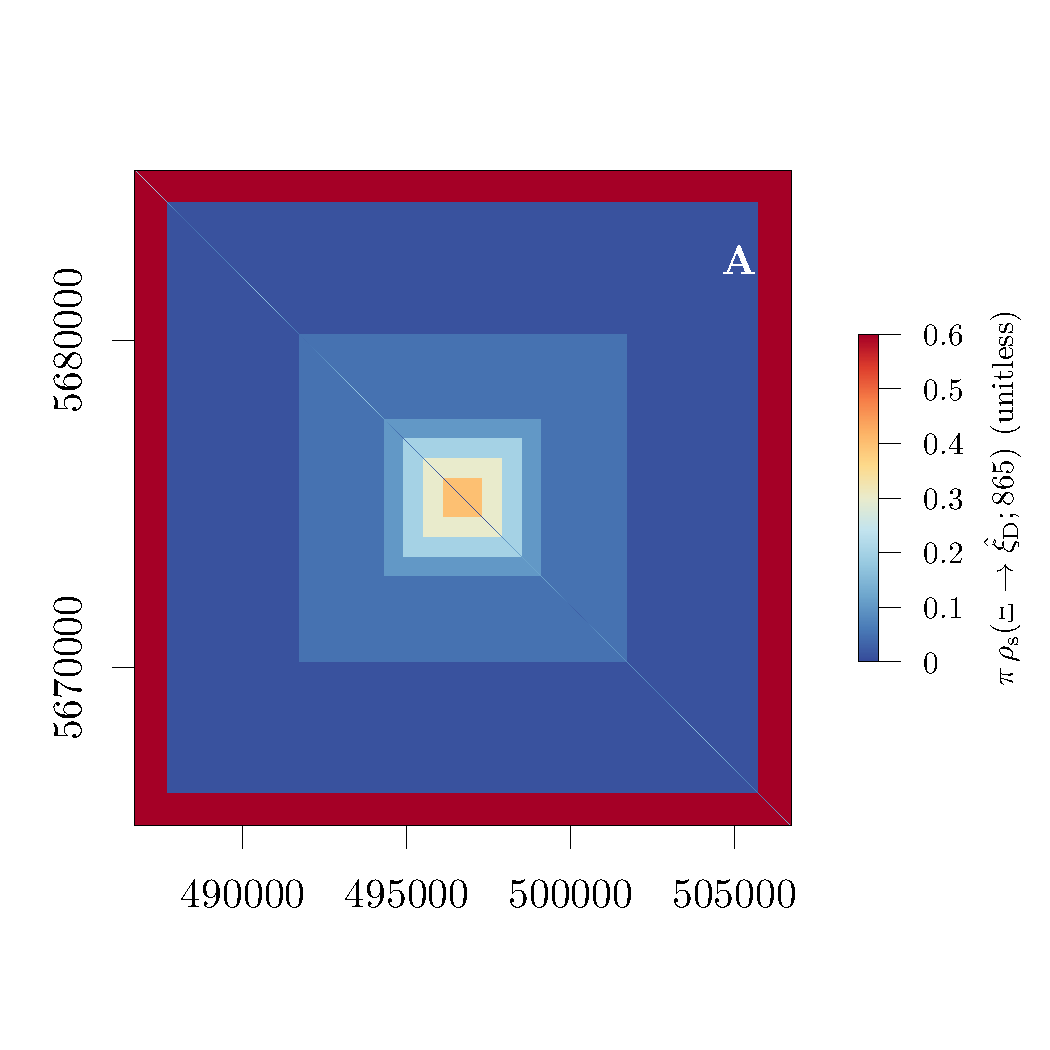
\includegraphics[trim={0 2cm 0 0},clip,width=\linewidth]{case_0_rho_s.pdf}
    \end{subfigure}
    \begin{subfigure}[t]{0.48\textwidth}
      \centering
      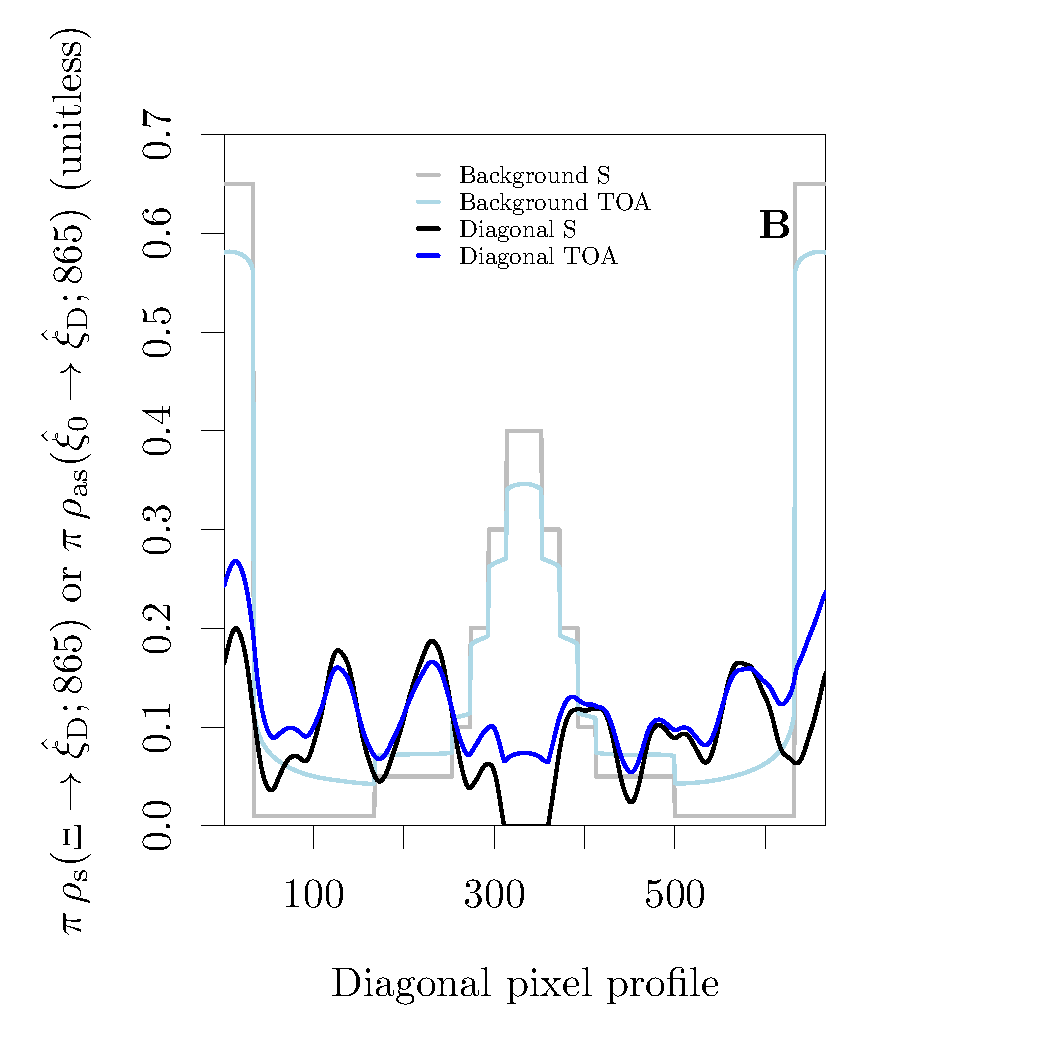
\includegraphics[trim={0 2cm 0 0},clip,width=\linewidth]{case_0_surface_profile.pdf}
    \end{subfigure}

  \vspace{0.1cm}

    \begin{subfigure}[t]{0.48\textwidth}
      \centering
      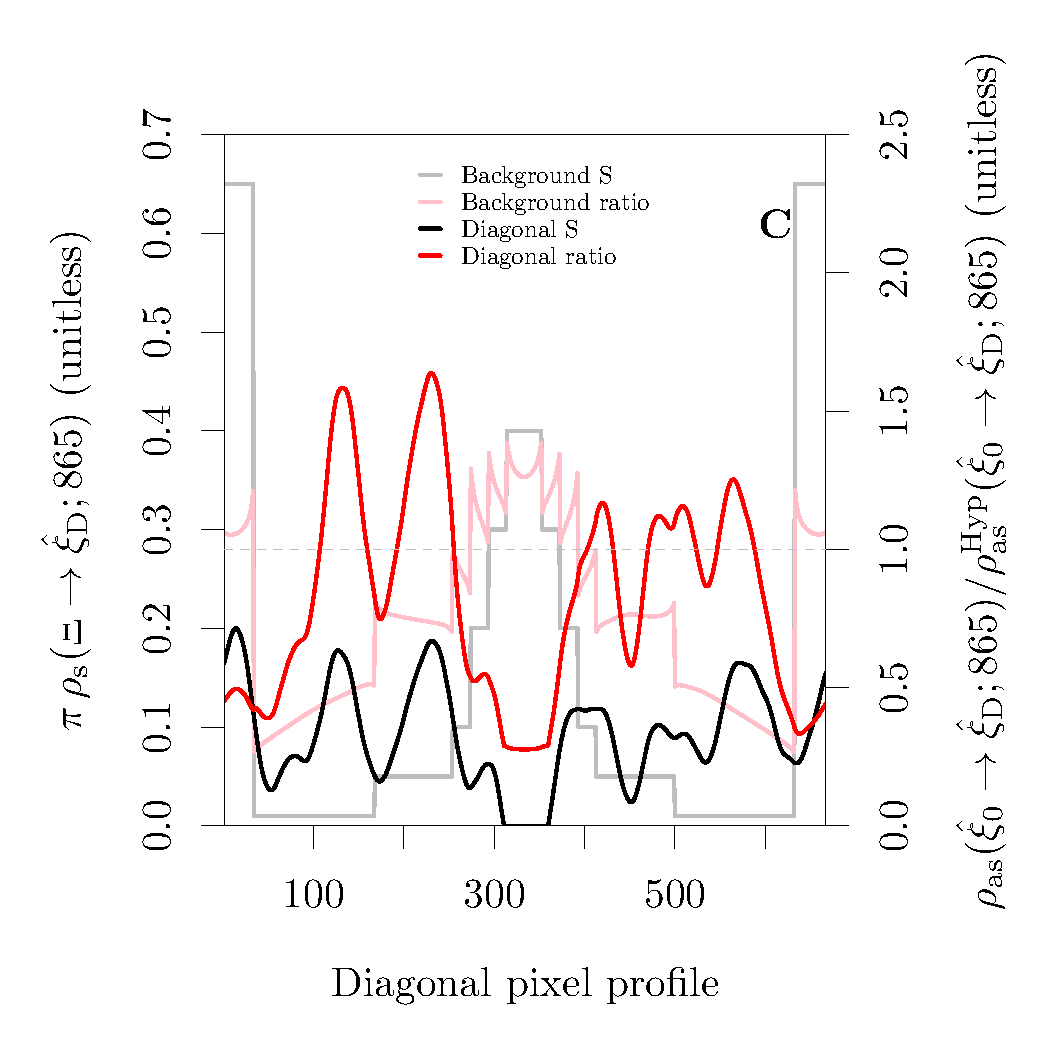
\includegraphics[trim={0 2cm 0 0},clip,width=\linewidth]{case_0_ratio_profile.pdf}
    \end{subfigure}
    \begin{subfigure}[t]{0.48\textwidth}
      \centering
      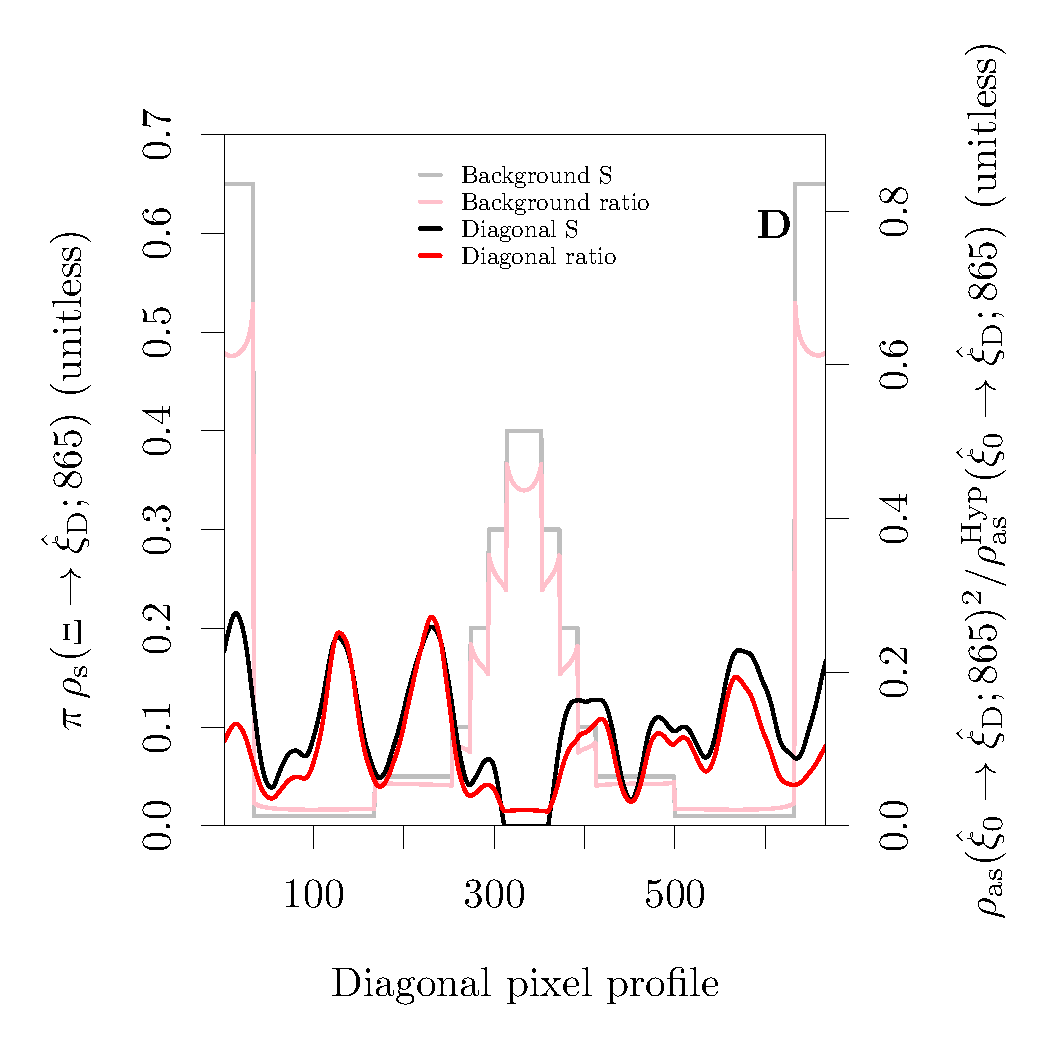
\includegraphics[trim={0 2cm 0 0},clip,width=\linewidth]{case_0_scaled_ratio_profile.pdf}
    \end{subfigure}

   \caption{Demonstration of finding the darkest pixel at the surface with the TSDSF. (A) Hemispherical-directional surface reflectance scaled by $\smash{\pi}$ sr$^{-1}$, $\smash{\pi \, \rho_\text{s}(\hemidn \rightarrow \hat{\xi}_\text{D})}$; (B) Hemispherical-directional of the surface and at TOA along the main diagonal, scaled by $\smash{\pi}$ sr$^{-1}$; (C) Hemispherical-directional of the surface scaled by $\smash{\pi}$ sr$^{-1}$ and the ratio $\smash{\rho_\text{as}(\hat{\xi}_0 \rightarrow \hat{\xi}_\text{D}; \Lambda_w; \vec{x}) / \rho_\text{as}^\text{Hyp}(\hat{\xi}_0 \rightarrow \hat{\xi}_\text{D}; \Lambda_w; \vec{x})}$; (D) Hemispherical-directional of the surface scaled by $\smash{\pi}$ sr$^{-1}$ and the scaled ratio $\smash{\rho_\text{as}(\hat{\xi}_0 \rightarrow \hat{\xi}_\text{D}; \Lambda_w; \vec{x})^2 / \rho_\text{as}^\text{Hyp}(\hat{\xi}_0 \rightarrow \hat{\xi}_\text{D}; \Lambda_w; \vec{x})}$. All variables presented for the NIR waveband of OLI, centred at wavelength 865~nm.}
   \label{fig:tsdsf_demo}
\end{figure}

Finally, the selection of the darkest pixel (lowest ratio) might lead to errors due to imagery artifacts (noise, detector malfunction, etc). As for standard DSF in ACOLITE, the ratio can be sorted and a given percentile value be chosen as reference value. The default in ACOLITE is the 1~\% darkest pixel.

% Subsection -------------------------------------------------------------------
\subsection{Estimation of aerosol properties}

The darkest pixels at the surface can then be used to estimate $\smash{\tau_\text{aer}(550)}$. We first define the dark spectra at TOA and for the hypothetical quantity from the darkest pixels in each waveband and the appropriate spatial functions. To simplify the notation, we will use $\smash{\rho_\text{as}^\text{SDark}(\hat{\xi}_0 \rightarrow \hat{\xi}_\text{D}; \Lambda_w)}$ and $\smash{\rho_\text{as}^\text{Hyp SDark}(\hat{\xi}_0 \rightarrow \hat{\xi}_\text{D}; \Lambda_w)}$ to identify the dark spectra. That is:

\begin{equation}
\rho_\text{as}^\text{SDark}(\hat{\xi}_0 \rightarrow \hat{\xi}_\text{D}; \Lambda_w) = \rho_\text{as}(\hat{\xi}_0 \rightarrow \hat{\xi}_\text{D}; \Lambda_w; \vec{x}_{\text{a}_\text{SDark}}(\Lambda_w)),
\end{equation}
\begin{equation}
\rho_\text{as}^\text{Hyp SDark}(\hat{\xi}_0 \rightarrow \hat{\xi}_\text{D}; \Lambda_w) = \rho_\text{as}^\text{Hyp}(\hat{\xi}_0 \rightarrow \hat{\xi}_\text{D}; \Lambda_w; \vec{x}_{\text{a}_\text{SDark}}(\Lambda_w)).
\end{equation}

By definition, the ratio of the path corrected $\smash{\rho_\text{as}(\hat{\xi}_0 \rightarrow \hat{\xi}_\text{D}; \Lambda_w; \vec{x})}$ to $\smash{\rho_\text{as}^\text{Hyp}(\hat{\xi}_0 \rightarrow \hat{\xi}_\text{D}; \Lambda_w; \vec{x})}$ for pixels with zero surface reflectance is equal to the relative upward diffuse transmittance. Therefore, by taking the dark spectra to represent the signal at TOA over pixels with 0 reflectance we have:

\begin{equation}
\frac{\rho_\text{pc}^\text{SDark}(\hat{\xi}_0 \rightarrow \hat{\xi}_\text{D}; \Lambda_w)}{\rho_\text{pc}^\text{Hyp SDark}(\hat{\xi}_0 \rightarrow \hat{\xi}_\text{D}; \Lambda_w)} = \frac{T_{\text{u}_\text{dif}}(\hemiup \rightarrow \hat{\xi}_\text{D}; \Lambda_w)}{T_{\text{u}_\text{tot}}(\hemiup \rightarrow \hat{\xi}_\text{D}; \Lambda_w)} + \varepsilon(\Lambda_w),
\label{eq:ret_ratio}
\end{equation}
\begin{equation}
\rho_\text{pc}^\text{SDark}(\hat{\xi}_0 \rightarrow \hat{\xi}_\text{D}; \Lambda_w) = \frac{\rho_\text{as}^\text{SDark}(\hat{\xi}_0 \rightarrow \hat{\xi}_\text{D}; \Lambda_w)}{T_\text{g}(\hat{\xi}_0; \hat{\xi}_\text{D}; \Lambda_w)} - \rho_\text{a}(\hat{\xi}_0 \rightarrow \hat{\xi}_\text{D}; \Lambda_w),
\end{equation}
\begin{equation}
\rho_\text{pc}^\text{Hyp SDark}(\hat{\xi}_0 \rightarrow \hat{\xi}_\text{D}; \Lambda_w) = \frac{\rho_\text{as}^\text{Hyp SDark}(\hat{\xi}_0 \rightarrow \hat{\xi}_\text{D}; \Lambda_w)}{T_\text{g}(\hat{\xi}_0; \hat{\xi}_\text{D}; \Lambda_w)} - \rho_\text{a}(\hat{\xi}_0 \rightarrow \hat{\xi}_\text{D}; \Lambda_w),
\end{equation}

\noindent where $\smash{\varepsilon(\Lambda_w)}$ is an error term related to non-zero surface reflectance, as in Eq.~\ref{eq:ts_dsf_rhoa}. Since $\smash{T_\text{g}}$ can be calculated based on external information, and $\smash{T_{\text{u}_\text{dif}}}$, $\smash{T_{\text{u}_\text{tot}}}$, and $\smash{\rho_\text{a}(\hat{\xi}_0 \rightarrow \hat{\xi}_\text{D})}$ are dependent on $\smash{\tau_\text{aer}(550)}$ for a given aerosol model, Eq.~\ref{eq:ret_ratio} can be solved with one unknown, $\smash{\tau_\text{aer}(550)}$. $\smash{\tau_\text{aer}(550)}$ is then estimated from Eq.~\ref{eq:ret_ratio} by optimisation, minimising the difference between the observed ratio and the predicted fractional diffuse transmittance for a given test value of $\smash{\rho_\text{a}(\hat{\xi}_0 \rightarrow \hat{\xi}_\text{D}; \Lambda_w)}$. The optimisation solution is constrained to $\smash{\tau_\text{aer}(550)}$ that would result at maximum in a $\smash{\rho_\text{a}(\hat{\xi}_0 \rightarrow \hat{\xi}_\text{D}; \Lambda_w)}$ equal to the darkest pixel at TOA corrected for gas transmittance, $\smash{\rho_\text{as}^{\text{TDark}}(\hat{\xi}_0 \rightarrow \hat{\xi}_\text{D}; \Lambda_w)/T_\text{g}(\hat{\xi}_0; \hat{\xi}_\text{D}; \Lambda_w)}$, preventing negative surface reflectances. The solution of Eq.~\ref{eq:ret_ratio} by optimisation requires no iteration of image processing. It operates only on the dark surface TOA spectrum and on LUT interpolation, resulting in considerable improvement on processing power over $\smash{\tau_\text{aer}(550)}$ estimations that require image processing iteration.

The integro-normalised atmospheric diffuse point spread function, $\smash{\hat{\curlywedge}_\text{b}^*(\hemiup \rightarrow \hat{\xi}_\text{D}; \Lambda_w; \vec{x})}$, used in Eq.~\ref{eq:est_rho_e_toa} depends on the aerosol model and on the relative contributions of Rayleigh and aerosol to the upward diffuse transmittance. Since the aerosol models available in the LUT will not exactly match the aerosol properties in the observed scene and the diffuse transmittance component due to aerosols is not known ahead of time, the error term $\smash{\varepsilon(\Lambda_w)}$ also includes the effects of those differences, besides any direct upward transmittance from the darkest pixel at the surface having non-zero reflectance. 

The effect of non-zero surface reflectances will produce a different estimation of $\smash{\tau_\text{aer}(550)}$ per waveband, and consequently of $\smash{\rho_\text{a}(\hat{\xi}_0 \rightarrow \hat{\xi}_\text{D}; \Lambda_w)}$. The spectra of the $\smash{\rho_\text{a}(\hat{\xi}_0 \rightarrow \hat{\xi}_\text{D}; \Lambda_w)}$ calculated from the $\smash{\tau_\text{aer}(550)}$ estimated at each waveband is the maximum path reflectance expected in each waveband for a given aerosol model, under the assumption that the surface reflectance is zero. We note, therefore, that this quantity is not equal to $\smash{\rho_\text{as}^{\text{TDark}}(\hat{\xi}_0 \rightarrow \hat{\xi}_\text{D}; \Lambda_w)/T_\text{g}(\hat{\xi}_0; \hat{\xi}_\text{D}; \Lambda_w)}$ as in the DSF approach (Eq.~\ref{eq:ts_dsf_rhoa}), and it will be represented hereafter by $\smash{\rho_\text{a}^\text{SDark}(\hat{\xi}_0 \rightarrow \hat{\xi}_\text{D}; \Lambda_w)}$.

The solution of Eq.~\ref{eq:ret_ratio} will provide one estimate of $\smash{\tau_\text{aer}(550)}$ per waveband and per aerosol model. As in DSF, the lowest $\smash{\tau_\text{aer}(550)}$ estimate for each aerosol model is selected. This ensures no negative surface reflectance retrievals. The selection of the aerosol model is then performed with a similar approach to the one used in DSF, but substituting $\smash{\rho_\text{as}^\text{TDark}(\hat{\xi}_0 \rightarrow \hat{\xi}_\text{D}; \Lambda_w)}$ by $\smash{\rho_\text{a}^\text{SDark}(\hat{\xi}_0 \rightarrow \hat{\xi}_\text{D}; \Lambda_w)}$. That is, the aerosol model is selected based on the best lower bound fit between the estimated $\smash{\rho_\text{a}(\hat{\xi}_0 \rightarrow \hat{\xi}_\text{D}; \Lambda_w)}$ spectrum for the lowest $\smash{\tau_\text{aer}(550)}$ and $\smash{\rho_\text{a}^\text{SDark}(\hat{\xi}_0 \rightarrow \hat{\xi}_\text{D}; \Lambda_w)}$. We note that an implicit assumption of this method is that the atmosphere's composition can be considered constant in the scene (or tile), an assumption used in the development of the equations in Chapter~\ref{ch:theory}.

We name this approach ``TOA and Surface Dark Spectra Fitting'' (TSDSF). Regardless of the option to process or not the ``edge area'' of the scene, the TSDSF uses only the ``centre area'' of the scene to estimate $\smash{\tau_\text{aer}(550)}$ and aerosol model (\textit{cf.} Chapter~\ref{ch:finite}). The pseudo-code of the TSDSF, including the compensation for the finite scene and kernels (\textit{cf.} Chapter~\ref{ch:finite}), is provided in the Appendix~\ref{ap:ts_dsf}.

Further details are provided in Chapters~\ref{ch:sim01} and~\ref{ch:sim02}, but we summarise here that this approach results in accurate retrievals of aerosol properties up to moderate turbidities ($\tau_\text{aer}(550) < 0.4$), i.e., for the typical cases where $\smash{T_{\text{u}_\text{dif}}(\hemiup \rightarrow \hat{\xi}_\text{D}) < T_{\text{u}_\text{dir}}(\hemiup \rightarrow \hat{\xi}_\text{D})}$ (\textit{cf.} Fig.~\ref{fig:psf_diffrat_spectral}).

\printendnotes[custom]


\chapter{Retrieval of surface reflectances} \label{ch:radcor}

With the aerosol properties provided externally or estimated from the imagery (\textit{e.g.}, Chapter~\ref{ch:ts_dsf}), the transmittances and reflectances terms of the atmosphere can be calculated with radiative transfer simulations for the observation geometry and a given standard atmospheric profile, or interpolated from a previously calculated LUT. These quantities can then be used with the appropriate measurement equation to retrieve the surface reflectance from the TOA observations.

As in Chapter~\ref{ch:ts_dsf}, we will consider that the scene extent is large enough around the region of interest to contain the full area contributing to the diffusely transmitted signal from the surface to the sensor for the region of interest. The consequences and adaptations necessary to handle spatially finite kernels and scenes will be developed in Chapter~\ref{ch:finite}. However, the dependency of the spectral response function $\Lambda_w$ will be dropped in the equations of this chapter to simplify the presentation, as no spectral analysis is necessary. 

\section{Retrieval over Homogeneous Lambertian surfaces}

The measurement equation over homogeneous Lambertian surfaces, Eq.~\ref{eq:theory_lambertian_homogeneous}, can be rearranged to solve for the surface reflectance. For the DSF approach and other approaches that consider the atmosphere's composition to be constant within a given spatial extent, $\smash{\rho_\text{s}(\vec{x})}$ can be retrieved in that extent as:

\begin{equation}
\openup 2\jot
\rho_\text{s}(\vec{x}_\text{b}) = \frac{ \rho_\text{pc}(\hat{\xi}_0 \rightarrow \hat{\xi}_\text{D}; \vec{x}_\text{a})}{T_{\text{d}_\text{tot}}(\hat{\xi}_0 \rightarrow \hemidn) \, T_{\text{u}_\text{tot}}(\hemiup \rightarrow \hat{\xi}_\text{D}) + \pi \, \rho_\text{pc}(\hat{\xi}_0 \rightarrow \hat{\xi}_\text{D}; \vec{x}_\text{a}) \, \rho_\text{b}(\hemiup \rightarrow \hemidn)},
\label{eq:radcor_hm_inversion}
\end{equation}

\begin{equation}
\rho_\text{pc}(\hat{\xi}_0 \rightarrow \hat{\xi}_\text{D}; \vec{x}_\text{a}) = \frac{\rho_\text{as}(\hat{\xi}_0 \rightarrow \hat{\xi}_\text{D}; \vec{x}_\text{a})}{T_\text{g}(\hat{\xi}_0; \hat{\xi}_\text{D})} - \rho_\text{a}(\hat{\xi}_0 \rightarrow \hat{\xi}_\text{D}),
\label{eq:radcor_path_corrected}
\end{equation} 

\noindent where $\smash{\rho_\text{pc}(\hat{\xi}_0 \rightarrow \hat{\xi}_\text{D}; \vec{x})}$ is known as the ``path corrected'' TOA reflectance and the $\pi$ factor (with units of sr) converts between directional and hemispherical reflectances for the Lambertian BRDF. For approaches that calculate per pixel $\tau_\text{aer}(550)$ and aerosol model (\textit{e.g.}, as typical for the ``dark pixel'' approach), the atmospheric transmittances and reflectances are modified to be spatial functions, \textit{e.g.}, $\smash{\rho_\text{a}(\hat{\xi}_0 \rightarrow \hat{\xi}_\text{D}; \vec{x}_\text{a})}$.

\section{Retrieval over Heterogeneous Lambertian surfaces}

The measurement equation over Lambertian surfaces, Eq.~\ref{eq:theory_me_closed_form}, cannot be rearranged to solve for $\smash{\rho_\text{s}(\vec{x})}$, as was done in Eq.~\ref{eq:radcor_hm_inversion}, due to the convolution in the denominator. Therefore, our approach is to approximate $\smash{\rho_{\text{s}_{\curlyvee_\text{b}}}(\hemidn \rightarrow \hemiup; \vec{x}_\text{b})}$ directly from the TOA scene, keeping the denominator as presented in Eq.~\ref{eq:theory_comp_II_III_C2}:

\begin{equation}
\openup 2\jot
1 - \bigr\{ \pi \, \rho_\text{s}(\hemidn \rightarrow \hat{\xi}_\text{D}; \vec{x}^\prime) \circledast \curlyvee_\text{b}(\hemiup \rightarrow \hemidn; \vec{x}^\prime) \bigr\} (\vec{x}_\text{b}) = 1 - \rho_{\text{s}_{\curlyvee_\text{b}}}(\hemidn \rightarrow \hemiup; \vec{x}_\text{b}) \, \rho_\text{b}(\hemiup \rightarrow \hemidn).
\label{eq:radcor_denominator}
\end{equation} 

Typically, $\smash{\rho_{\text{s}_{\curlyvee_\text{b}}}(\hemidn \rightarrow \hemiup; \vec{x}_\text{b}) \, \rho_\text{b}(\hemiup \rightarrow \hemidn)}$ is lower than 10~\%, so uncertainties in $\smash{\rho_{\text{s}_{\curlyvee_\text{b}}}(\hemidn \rightarrow \hemiup; \vec{x}_\text{b})}$ will have a minor impact on the estimate of $\smash{\rho_\text{s}(\vec{x}_\text{b})}$. We estimate $\smash{\rho_{\text{s}_{\curlyvee_\text{b}}}(\hemidn \rightarrow \hemiup; \vec{x}_\text{b})}$ by first applying the integro-normalised SAF to the signal at TOA:

\begin{equation}
\openup 2\jot
\frac{\rho_{\text{as}_{\curlyvee_\text{b}}}(\hemidn \rightarrow \hemiup; \vec{x}_\text{a})}{T_\text{g}(\hat{\xi}_0; \hat{\xi}_\text{D})} = \frac{\pi \, \rho_\text{as}(\hat{\xi}_0 \rightarrow \hat{\xi}_\text{D}; \vec{x}_\text{a})}{T_\text{g}(\hat{\xi}_0; \hat{\xi}_\text{D})} \circledast \hat{\curlyvee}_\text{b}(\hemiup \rightarrow \hemidn; \vec{x}_\text{a}),
\label{eq:radcor_rho_env_sph_toa}
\end{equation}

\begin{equation}
\openup 2\jot
\hat{\curlyvee}_\text{b}(\hemiup \rightarrow \hemidn; \vec{x}) = \frac{\curlyvee_\text{b}(\hemiup \rightarrow \hemidn; \vec{x})}{\rho_\text{b}(\hemiup \rightarrow \hemidn)}.
\label{eq:radcor_unit_saf}
\end{equation}

We can then estimate $\smash{\rho_{\text{s}_{\curlyvee_\text{b}}}(\hemidn \rightarrow \hemiup; \vec{x}_\text{b})}$ with an equation similar to Eq.~\ref{eq:radcor_hm_inversion}, as:

\begin{equation}
\openup 2\jot
\rho_{\text{s}_{\curlyvee_\text{b}}}(\hemidn \rightarrow \hemiup; \vec{x}_\text{b}) \approx \frac{\rho_{\text{pc}_{\curlyvee_\text{b}}}(\hemidn \rightarrow \hemiup; \vec{x}_\text{a})}{T_{\text{d}_\text{tot}}(\hat{\xi}_0 \rightarrow \hemidn) \, T_{\text{u}_\text{tot}}(\hemiup \rightarrow \hat{\xi}_\text{D}) + \rho_{\text{pc}_{\curlyvee_\text{b}}}(\hemidn \rightarrow \hemiup; \vec{x}_\text{a}) \, \rho_\text{b}(\hemiup \rightarrow \hemidn)},
\label{eq:radcor_rho_env_sph}
\end{equation} 

\begin{equation}
\rho_{\text{pc}_{\curlyvee_\text{b}}}(\hemidn \rightarrow \hemiup; \vec{x}_\text{a}) = \frac{\rho_{\text{as}_{\curlyvee_\text{b}}}(\hemidn \rightarrow \hemiup; \vec{x}_\text{a})}{T_\text{g}(\hat{\xi}_0; \hat{\xi}_\text{D})} - \pi \, \rho_\text{a}(\hat{\xi}_0 \rightarrow \hat{\xi}_\text{D}).
\label{eq:radcor_rho_env_sph_pc}
\end{equation}

The approximation is justified on the grounds that $\smash{\hat{\curlyvee}_\text{b}(\hemiup \rightarrow \hemidn; \vec{x})}$ has a much larger spatial scale than the diffuse PSF and causes intense blurring, strongly reducing the spatial contrast and reducing the calculations to the homogeneous surface case. 

With the estimated $\smash{\rho_{\text{s}_{\curlyvee_\text{b}}}(\hemidn \rightarrow \hemiup;\vec{x}_\text{b})}$, it is possible to solve Eq.~\ref{eq:theory_me_closed_form} for $\smash{\rho_\text{s}(\vec{x}_\text{b})}$ with:

\begin{equation}
\openup 2\jot
\rho_\text{s}(\vec{x}_\text{b}) = \frac{1 -\rho_{\text{s}_{\curlyvee_\text{b}}}(\hemidn \rightarrow \hemiup; \vec{x}_\text{b}) \, \rho_\text{b}(\hemiup \rightarrow \hemidn)}{\pi \, T_{\text{d}_\text{tot}}(\hat{\xi}_0 \rightarrow \hemidn)} \, \mathcal{F}^{-1}\Biggr\{\frac{\mathcal{F}\Bigr\{\rho_\text{pc}(\hat{\xi}_0 \rightarrow \hat{\xi}_\text{D}; \vec{x}_\text{a}) \Bigr\}}{\mathcal{F}\Bigr\{\curlywedge_\text{b}\!(\hemiup \rightarrow \hat{\xi}_\text{D}; \vec{x})\Bigr\}}\Biggr\},
\label{eq:radcor_lambertian_scene_fourier}
\end{equation} 

\noindent where $\smash{\mathcal{F}}$ indicates the Fourier transform, $\smash{\mathcal{F}^{-1}}$ indicates the inverse Fourier transform, and we use the convolution theorem to convert the convolution in spatial domain to multiplication in the frequency domain. Therefore, if $\smash{\rho_{\text{s}_{\curlyvee_\text{b}}}(\hemidn \rightarrow \hemiup; \vec{x})}$ can be approximated, and the scene is large enough to cover 100~\% of $\smash{\curlywedge_\text{b}^*(\hemiup \rightarrow \hat{\xi}_\text{D}; \vec{x})}$ for the area of interest, it is possible to retrieve $\smash{\rho_\text{s}(\vec{x})}$ from knowledge of atmospheric optical properties.

The pseudo-code of RAdCor is provided in Appendix~\ref{ap:radcor}.


\chapter{Finite spatial extents} \label{ch:finite}

The spatial scale of the $\smash{\curlyvee_\text{b}(\hemiup \rightarrow \hemidn; \vec{x})}$ and $\smash{\curlywedge_\text{b}^*(\hemiup \rightarrow \hat{\xi}_\text{D}; \vec{x})}$ kernels is on the order of several kilometres (\textit{cf.} Fig.~\ref{fig:sph_albd_sim_res} and Fig.~\ref{fig:psf_sim_res}). In the spectral range from the visible to the SWIR, a $\tau_\text{aer}(550)$ from 0 to 0.3~(unitless) requires a kernel radius from 10~km to 60~km radius to cover $\approx$ 100~\% of the area contributing to the signal over a pixel. Consequently, the extent of the kernels can be larger than the scene and is larger than the spatial scale in which spatial homogeneity of the atmosphere composition is a reasonable assumption ($\approx 3.5$~km radius). Therefore, to retrieve surface reflectance it is necessary to work with finite and truncated spatial kernels \citep{Reinersman1995}.

The condition described above is presented schematically in Fig.~\ref{fig:finite_finite}, using the diffuse PSF as the example kernel. The finite scene and PSF extents will result in a ``centre area'' and in an ``edge area''. The centre area is defined by pixels more than half the PSF extent away from the scene border, while the edge area is the complement. The consequence of the finite extents are:

\begin{enumerate}
  \item The integro-normalised kernels no longer integrate to unity in their finite extents.
  \item The edge area of the scene does not contain enough surrounding pixels to be processed even with the finite kernels.
\end{enumerate}

\begin{figure}[!htbp]
  \centering
  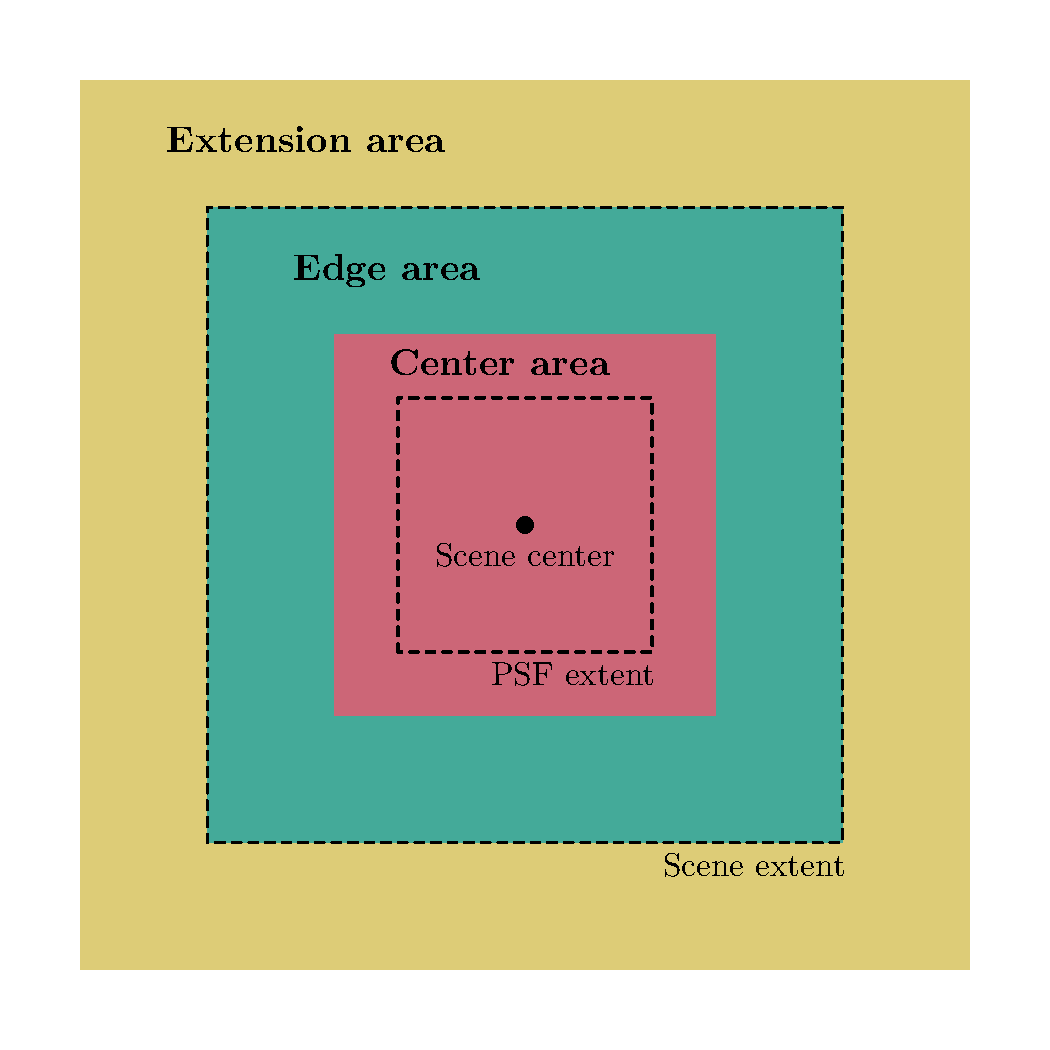
\includegraphics[width=0.5\linewidth]{finite}
  \caption{Schematic representation of the scene. Traced line represent the borders of the finite truncated diffuse PSF and of the finite scene.}
  \label{fig:finite_finite}
\end{figure}

In this chapter we will consider the approximations necessary to deal with these two consequences, expanding upon the suggestions of \cite{Reinersman1995}.

% Section -------------------------------------------------------------------
\section{Incomplete spatial kernels}

We define $B_\text{in}$ as the surface area covered by the truncated kernels. We can then define the truncated kernels $\smash{\bunderline[4]{\curlyvee}_\text{b}(\hemiup \rightarrow \hemidn; \vec{x})}$ and $\smash{\bunderline[4]{\curlywedge}_\text{b}^*(\hemiup \rightarrow \hat{\xi}_\text{D}; \vec{x})}$ as:

\begin{equation}
\bunderline[4]{\curlyvee}_\text{b}(\hemiup \rightarrow \hemidn; \vec{x}) =
\begin{cases}
    \curlyvee_\text{b}(\hemiup \rightarrow \hemidn; \vec{x}),& \text{if } \vec{x} \in B_\text{in}\\
    0,              & \text{otherwise}
\end{cases},
\end{equation}

\begin{equation}
\bunderline[4]{\curlywedge}_\text{b}^*(\hemiup \rightarrow \hat{\xi}_\text{D}; \vec{x}) =
\begin{cases}
    \curlywedge_\text{b}^*(\hemiup \rightarrow \hat{\xi}_\text{D}; \vec{x}),& \text{if } \vec{x} \in B_\text{in}\\
    0,              & \text{otherwise}
\end{cases}.
\label{eq:finite_trunc_dif_psf}
\end{equation}

We note that while all the functions presented in this chapter vary with the sensor waveband $w$, the dependency of the relative spectral response function, $\Lambda_w$, is dropped to simplify the presentation. 

Other useful quantities are the fractions of the spherical albedo $\smash{\rho_\text{b}(\hemiup \rightarrow \hemidn)}$ and hemispherical-directional upward transmittance $\smash{T_{\text{u}_\text{tot}}(\hemiup \rightarrow \hat{\xi}_\text{D})}$ that are covered in the finite extent of the kernels:

\begin{equation}
f_{\curlyvee_\text{b}} = \int\limits_{B} d\vec{x} \,\,\, \bunderline[4]{\hat{\curlyvee}}_\text{b}(\hemiup \rightarrow \hemidn; \vec{x}),
\end{equation}

\begin{equation}
f_{\curlywedge_\text{b}^*} = \int\limits_{B} d\vec{x} \,\,\, \bunderline[4]{\hat{\curlywedge}}_\text{b}^*(\hemiup \rightarrow \hat{\xi}_\text{D}; \vec{x}).
\end{equation} 

The simplest approximation to account for the finite kernels is the re-normalisation given by:

\begin{equation}
\frac{\bunderline[4]{\hat{\curlyvee}}_\text{b}(\hemiup \rightarrow \hemidn; \vec{x})}{f_{\curlyvee_\text{b}}} \quad\quad\text{and}\quad\quad\frac{\bunderline[4]{\hat{\curlywedge}}_\text{b}^*(\hemiup \rightarrow \hat{\xi}_\text{D}; \vec{x})}{f_{\curlywedge_\text{b}^*}}.
\end{equation}

The re-normalisation approach, however, will overemphasise the contributions of pixels closer to the target pixel since the kernels are peaked in the center pixel. As a consequence, it will generally underestimate the adjacency effect, except in the immediacy of surface patch transitions.

Alternatively, we can account for finite extent of the kernels by adding the missing fractions $\smash{1 - f_{\curlyvee_\text{b}}}$ and $\smash{1 - f_{\curlywedge_\text{b}^*}}$ as scaling factors of averaged spatial quantities. For example, the finite version of Eq.~\ref{eq:est_rho_e_toa} is:

\begin{equation}
\openup 2\jot
\begin{split}
&\frac{\rho_\text{as}^\text{Hyp}(\hat{\xi}_0 \rightarrow \hat{\xi}_\text{D}; \vec{x})}{T_\text{g}(\hat{\xi}_0; \hat{\xi}_\text{D})} \approx \\
&\quad\quad\quad\left\{ \frac{\rho_\text{as}(\hat{\xi}_0 \rightarrow \hat{\xi}_\text{D}; \vec{x}^\prime)}{T_\text{g}(\hat{\xi}_0; \hat{\xi}_\text{D})} \circledast \bunderline[4]{\hat{\curlywedge}}_\text{b}^*(\hemiup \rightarrow \hat{\xi}_\text{D}; \vec{x}) \right\}(\vec{x}) \\
&\quad\quad+\left\{ \frac{\rho_\text{as}(\hat{\xi}_0 \rightarrow \hat{\xi}_\text{D}; \vec{x}^\prime)}{T_\text{g}(\hat{\xi}_0; \hat{\xi}_\text{D})} \circledast \left[ \hat{\curlywedge}_\text{b}^*(\hemiup \rightarrow \hat{\xi}_\text{D}; \vec{x}^\prime) - \bunderline[4]{\hat{\curlywedge}}_\text{b}^*(\hemiup \rightarrow \hat{\xi}_\text{D}; \vec{x}) \right] \right\}(\vec{x}) \\
& \\
&\quad\quad\approx \left\{ \frac{\rho_\text{as}(\hat{\xi}_0 \rightarrow \hat{\xi}_\text{D}; \vec{x}^\prime)}{T_\text{g}(\hat{\xi}_0; \hat{\xi}_\text{D})} \circledast \bunderline[4]{\hat{\curlywedge}}_\text{b}^*(\hemiup \rightarrow \hat{\xi}_\text{D}; \vec{x}) \right\}(\vec{x}) \\
&\quad\quad+\left\{ \frac{\rho_\text{as}(\hat{\xi}_0 \rightarrow \hat{\xi}_\text{D}; \vec{x}^\prime)}{T_\text{g}(\hat{\xi}_0; \hat{\xi}_\text{D})} \circledast \hat{U} \, \left[ 1 - f_{\curlywedge_\text{b}^*} \right] \right\}(\vec{x}),
\end{split}
\label{eq:finite_rho_e_toa}
\end{equation}

\noindent where $\smash{\hat{U}}$ is a integro-normalised uniform kernel of the same extent as $\smash{\bunderline[4]{\curlywedge}_\text{b}^*(\hemiup \rightarrow \hat{\xi}_\text{D}; \vec{x})}$. The convolution with the uniform kernel results in a ``local'' arithmetic average. Similarly, the finite version of Eq.~\ref{eq:radcor_rho_env_sph_toa} is:

\begin{equation}
\openup 2\jot
\begin{split}
\frac{\rho_{\text{as}_{\curlyvee_\text{b}}}(\hemidn \rightarrow \hemiup; \vec{x})}{T_\text{g}(\hat{\xi}_0; \hat{\xi}_\text{D})} &= \frac{\pi \, \rho_\text{as}(\hat{\xi}_0 \rightarrow \hat{\xi}_\text{D}; \vec{x})}{T_\text{g}(\hat{\xi}_0; \hat{\xi}_\text{D})} \circledast \bunderline[4]{\hat{\curlyvee}}_\text{b}(\hemiup \rightarrow \hemidn; \vec{x}) \\
&+ \frac{\pi \, \rho_\text{as}(\hat{\xi}_0 \rightarrow \hat{\xi}_\text{D}; \vec{x})}{T_\text{g}(\hat{\xi}_0; \hat{\xi}_\text{D})} \circledast \left[\hat{\curlyvee}_\text{b}(\hemiup \rightarrow \hemidn; \vec{x}) - \bunderline[4]{\hat{\curlyvee}}_\text{b}(\hemiup \rightarrow \hemidn; \vec{x})\right] \\
& \\
&\approx \frac{\pi \, \rho_\text{as}(\hat{\xi}_0 \rightarrow \hat{\xi}_\text{D}; \vec{x})}{T_\text{g}(\hat{\xi}_0; \hat{\xi}_\text{D})} \circledast \bunderline[4]{\hat{\curlyvee}}_\text{b}(\hemiup \rightarrow \hemidn; \vec{x}) \\
&+ \frac{\pi \, \rho_\text{as}(\hat{\xi}_0 \rightarrow \hat{\xi}_\text{D}; \vec{x})}{T_\text{g}(\hat{\xi}_0; \hat{\xi}_\text{D})} \circledast \hat{U} \, \left[1 - f_{\curlyvee_\text{b}}\right],
\end{split}
\label{eq:finite_rho_env_sph_toa}
\end{equation}

\noindent which allows for the estimation of $\smash{\rho_{\text{s}_{\curlyvee_\text{b}}}(\hemidn \rightarrow \hemiup; \vec{x}_\text{b})}$ with Eq.~\ref{eq:radcor_rho_env_sph} when considering finite images and truncated kernels.

In RAdCor we term the approach using the uniform kernel the ``neighborhood'' (``local'' average) complete method. A similar approach is possible with the ``global'' scene average (covering the centre area of the scene), which we term the ``average'' complete method. Preliminary evaluation of the code with data over inland water systems in Belgium showed a better performance with the neighbourhood complete method.

Finally, to retrieve the surface reflectances under finite scenes and truncated kernels, it is necessary to remove the missing fraction of the signal before the application of Eq.~\ref{eq:radcor_lambertian_scene_fourier}. We start by restating  Eq.~\ref{eq:theory_me_closed_form} in a more convenient format:

\begin{equation}
\openup 2\jot
\begin{split}
&\rho_\text{pc}(\hat{\xi}_0 \rightarrow \hat{\xi}_\text{D}; \vec{x}) = \\
&\, T_{\text{d}_\text{tot}}(\hat{\xi}_0 \rightarrow \hemidn) \frac{\rho_\text{s}(\vec{x})}{1 -\rho_{\text{s}_{\curlyvee_\text{b}}}(\hemidn \rightarrow \hemiup; \vec{x}) \, \rho_\text{b}(\hemiup \rightarrow \hemidn)} \circledast \pi \, \bunderline[4]{\curlywedge}_\text{b}(\hemiup \rightarrow \hat{\xi}_\text{D}; \vec{x}) \\
&\,+ T_{\text{d}_\text{tot}}(\hat{\xi}_0 \rightarrow \hemidn) \frac{\rho_\text{s}(\vec{x})}{1 -\rho_{\text{s}_{\curlyvee_\text{b}}}(\hemidn \rightarrow \hemiup; \vec{x}) \, \rho_\text{b}(\hemiup \rightarrow \hemidn)} \circledast \pi \left[ \curlywedge_\text{b}(\hemiup \rightarrow \hat{\xi}_\text{D};\vec{x}) - \bunderline[4]{\curlywedge}_\text{b}(\hemiup \rightarrow \hat{\xi}_\text{D}; \vec{x}) \right],
\end{split}
\label{eq:finite_me_closed_form}
\end{equation} 

\noindent where $\smash{\rho_\text{pc}(\hat{\xi}_0 \rightarrow \hat{\xi}_\text{D}; \vec{x})}$ is given by Eq.~\ref{eq:radcor_path_corrected}, and $\smash{\bunderline[4]{\curlywedge}_\text{b}(\hemiup \rightarrow \hat{\xi}_\text{D}; \vec{x})}$ is defined in a similar manner to Eq.~\ref{eq:finite_trunc_dif_psf}, but for the full PSF. We can then estimate the truncated path reflectance, $\smash{\bunderline[2]{\rho}_\text{pc}(\hat{\xi}_0 \rightarrow \hat{\xi}_\text{D}; \vec{x})}$, as:

\begin{equation}
\openup 2\jot
\begin{split}
&\bunderline[2]{\rho}_\text{pc}(\hat{\xi}_0 \rightarrow \hat{\xi}_\text{D}; \vec{x}) = \rho_\text{pc}(\hat{\xi}_0 \rightarrow \hat{\xi}_\text{D}; \vec{x}) \\
&\,- T_{\text{d}_\text{tot}}(\hat{\xi}_0 \rightarrow \hemidn) \frac{\rho_\text{s}(\vec{x})}{1 -\rho_{\text{s}_{\curlyvee_\text{b}}}(\hemidn \rightarrow \hemiup; \vec{x}) \, \rho_\text{b}(\hemiup \rightarrow \hemidn)} \circledast \pi \left[ \curlywedge_\text{b}(\hemiup \rightarrow \hat{\xi}_\text{D};\vec{x}) - \bunderline[4]{\curlywedge}_\text{b}(\hemiup \rightarrow \hat{\xi}_\text{D}; \vec{x}) \right] \\
& \\
&\,\approx \rho_\text{pc}(\hat{\xi}_0 \rightarrow \hat{\xi}_\text{D}; \vec{x}) - \rho_\text{pc}(\hat{\xi}_0 \rightarrow \hat{\xi}_\text{D}; \vec{x}) \circledast \hat{U} \left[1 - f_{\curlywedge_\text{b}^*}\right] \, T_{\text{u}_\text{dif}}(\hemiup \rightarrow \hat{\xi}_\text{D}).
\end{split}
\label{eq:finite_path}
\end{equation} 

The retrieval of surface reflectance is then given by:

\begin{equation}
\openup 2\jot
\rho_\text{s}(\vec{x}) = \frac{1 -\rho_{\text{s}_{\curlyvee_\text{b}}}(\hemidn \rightarrow \hemiup; \vec{x}) \, \rho_\text{b}(\hemiup \rightarrow \hemidn)}{T_{\text{d}_\text{tot}}(\hat{\xi}_0 \rightarrow \hemidn)} \, \mathcal{F}^{-1}\Biggr\{\frac{\mathcal{F}\Bigr\{\bunderline[2]{\rho}_\text{pc}(\hat{\xi}_0 \rightarrow \hat{\xi}_\text{D}; \vec{x}) \Bigr\}}{\mathcal{F}\Bigr\{\pi \, \bunderline[4]{\curlywedge}_\text{b}(\hemiup \rightarrow \hat{\xi}_\text{D}; \vec{x})\Bigr\}}\Biggr\}.
\label{eq:radcor_lambertian_scene_fourier_finite}
\end{equation} 

The approximation proposed above by using the uniform kernel differs from the re-normalisation by not further emphasising the immediacy of the target pixel, despite both using the information over the same spatial extent. This is expected to be more representative since the missing fractions $\smash{1 - f_{\curlyvee_\text{b}}}$ and $\smash{1 - f_{\curlywedge_\text{b}^*}}$ are in the edges of the peaked kernels (that is, would result in averages over large spatial extents). We note that other averages could be used, as for example the constant scene average (``global'' average). However, though in theory it could provide a better representation for a average over a large spatial scale, it will introduce artefacts in the imagery (\textit{e.g.} in a coastal scene, where half the image is ocean and the other half is land, the scene average is representative of neither).

% Section -------------------------------------------------------------------
\section{Incomplete surrounding areas}

The equations above only apply to the centre area of the scene, where the information necessary for the convolution with the finite spatial kernels is available. It is only possible to process the edge area if assumptions are made for the reflectance of the surfaces beyond the image extent, which is termed ``expansion area'' in Fig.~\ref{fig:finite_finite}, and defined by all pixels between the scene border and half the PSF extent beyond the scene border.

When the surface elements are well distributed in the scene, the average TOA signal over the scene can be used as a constant extrapolation of the signal for the extension area. However, when the scene contains large surfaces concentrated near the borders (\textit{e.g.} a coastal scene), mirrored images of the scene can be used to expand the scene in each direction. Both those options are implemented in RAdCor, though the default recommendation is to keep only the centre area as it requires no further assumptions of the reflectance of surface areas beyond the scene extent. Processing the edge area also increases computational time, as the image is extended. Despite those shortcomings, processing the edge might be necessary for regions of interest consistently imaged near the edge of a swath for global observation missions (e.g., MSI/Sentinel-2), or in scenes from commercial very high spatial resolution sensors if the available sensor capability or budget does not allow to acquire imagery over an extended area that would allow to discard the edge.

\section{Consequences of spatial finite kernels in EO}

Due to the symmetrical nature if the Rayleigh scattering phase function with regards to the scattering angle, the higher the Rayleigh contribution to the upward diffuse transmittance relative to the contribution of aerosols, the larger the radius of the kernel. Therefore, the lower the $\tau_\text{aer}(550)$ and the lower the wavelength, the larger the radius of the kernels. This implies that in general, wavebands centred more towards the blue end of the spectrum will have a larger error in the estimation of the environmental functions. Nonetheless, the contrast between vegetation and water is lower in the visible than in the NIR and SWIR, hence uncertainties in the retrieved reflectance in the visible range are comparable or even lower than those in the NIR to SWIR range. It also should be noted that the lower the $\tau_\text{aer}(550)$, the lower the contribution of those environmental functions to the recorded signal, therefore higher uncertainties on the atmospheric functions do not fully propagate to the estimation of surface reflectance.





\chapter{Evaluation: Simulated scene 1} \label{ch:sim01}

The first evaluation of the atmospheric correction scheme is performed with an inland simulated scene, such that the surface and atmospheric variables are known, with a simplified spatial pattern for the surface reflectance. Calculations are performed with Eq.~\ref{eq:theory_me_closed_form} to simulate the signal that would be observed over the Blankaart reservoir in Belgium, with the Operational Land Imager (OLI) onboard Landsat 8. The scene contains only two types of targets: water and vegetation (Fig.~\ref{fig:sim01_surf_setup}A). Water is represented by the Blankaart reservoir, an hexagonal water treatment plant with a radius of 450~m, and the Blankaart lake, with a irregular shape (Fig.~\ref{fig:sim01_surf_setup}B). The distance between the water systems is $\approx$ 1~km. All other positions of the infinite plane scene represent vegetation. 

\begin{figure}[!htbp]
  \centering
    \begin{subfigure}[t]{0.48\textwidth}
      \centering
      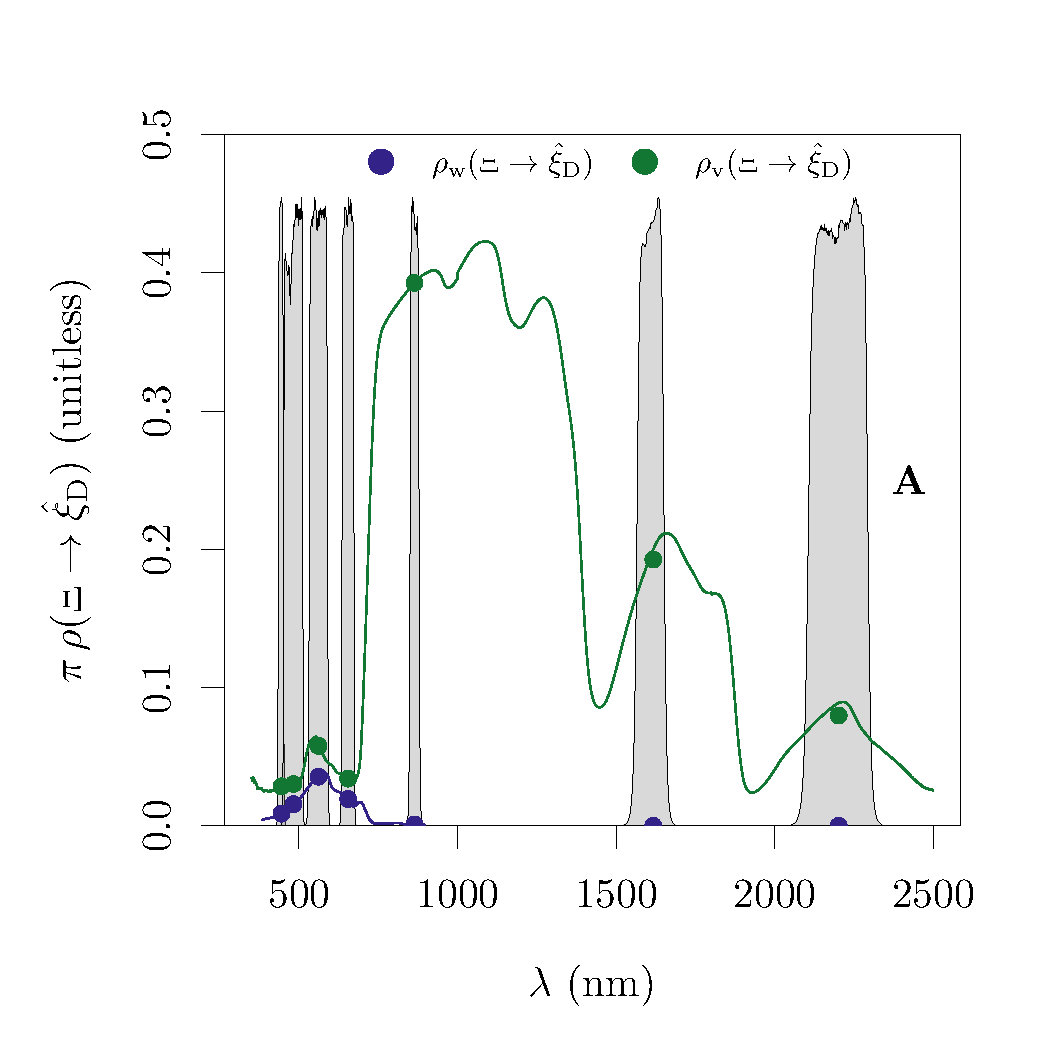
\includegraphics[trim={0 0.75cm 0 1cm},clip,width=\linewidth]{base_spectra.pdf}
    \end{subfigure}
    \begin{subfigure}[t]{0.48\textwidth}
      \centering
      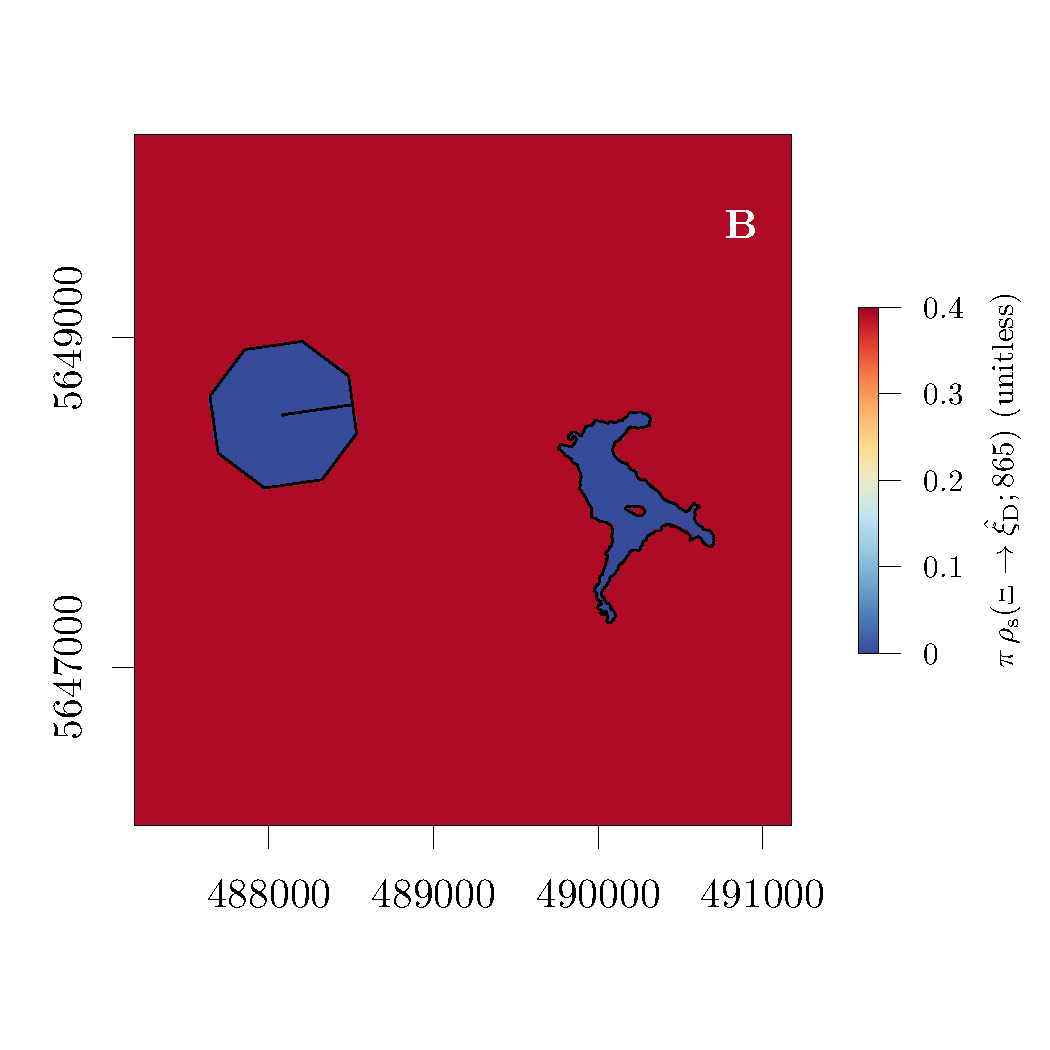
\includegraphics[trim={0 0.75cm 0 1cm},clip,width=\linewidth]{case_1_rho_s.pdf}
    \end{subfigure}
   \caption{Surface reflectance used in the simulation. (A) Spectral hemispherical-directional reflectance of surface targets, scaled by $\smash{\pi}$~sr. (B) Surface pattern of the hemispherical-directional surface reflectance scaled by $\smash{\pi}$~sr for the near-infrared waveband of OLI. In (A), subscript `w' stands for `water' and subscript `v' stands for `vegetation'. The grey polygons in the background show the relative spectral response functions of the first seven OLI wavebands.}
   \label{fig:sim01_surf_setup}
\end{figure}

The properties of the atmosphere were calculated with the 6SV code, using an atmospheric pressure at the surface of 1013.25~HPa and two standard aerosol models included in 6SV: continental and maritime. Those are the same aerosol models included in ACOLITE. The sun zenith angle was set to 32$^\circ$ and the view angle to nadir. The waveband average upward diffuse transmittance and spherical albedo for this atmosphere configuration is presented in Fig.~\ref{fig:sim01_atm_setup} for an $\smash{\tau_\text{aer}(865)}$ of 0.18~(unitless). This $\smash{\tau_\text{aer}(865)}$ corresponds to an $\smash{\tau_\text{aer}(550)}$ of 0.3~(unitless) for the continental aerosol model and to an $\smash{\tau_\text{aer}(550)}$ of 0.2~(unitless) for the maritime aerosol model.

\begin{figure}[!htbp]
  \centering
    \begin{subfigure}[t]{0.48\textwidth}
      \centering
      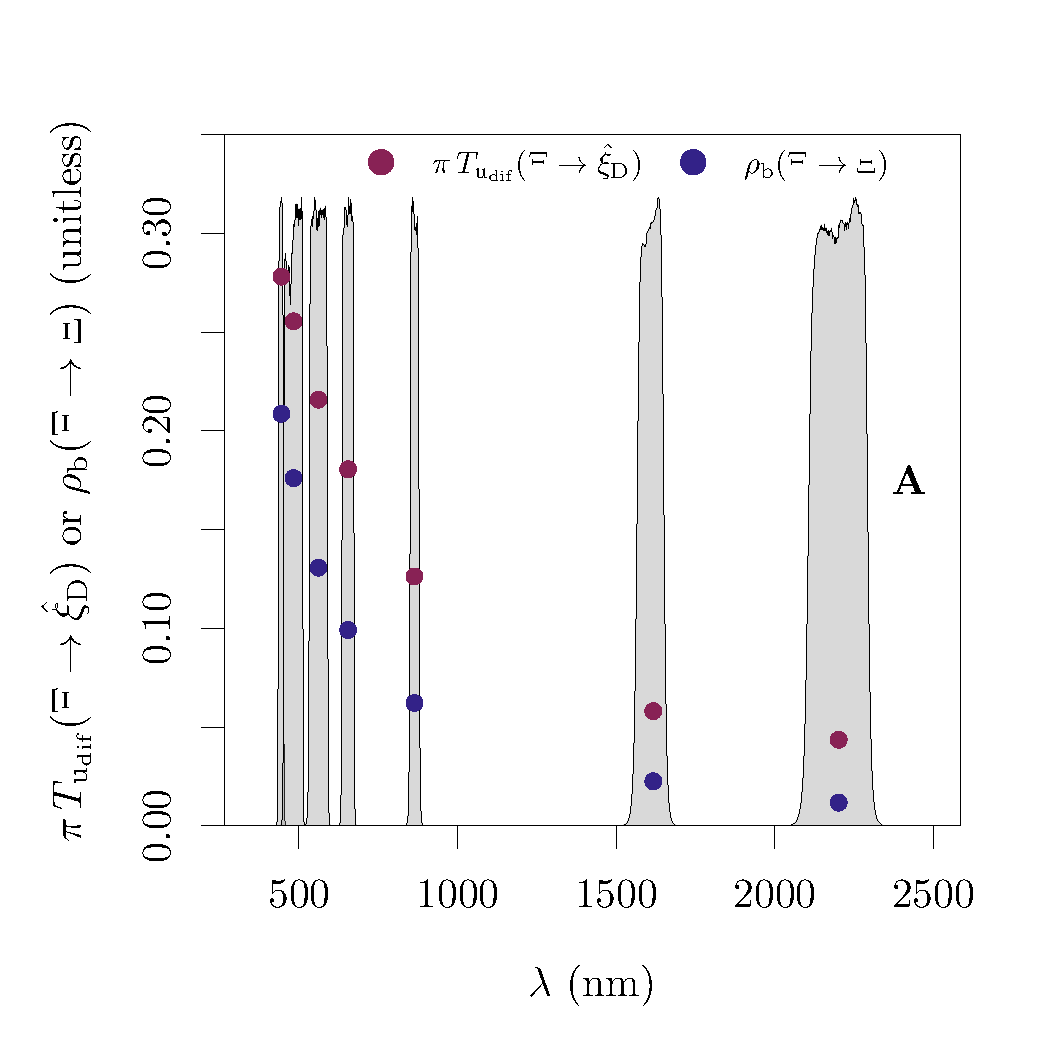
\includegraphics[trim={0 0.75cm 0 1cm},clip,width=\linewidth]{T_spectra_c.pdf}
    \end{subfigure}
    \begin{subfigure}[t]{0.48\textwidth}
      \centering
      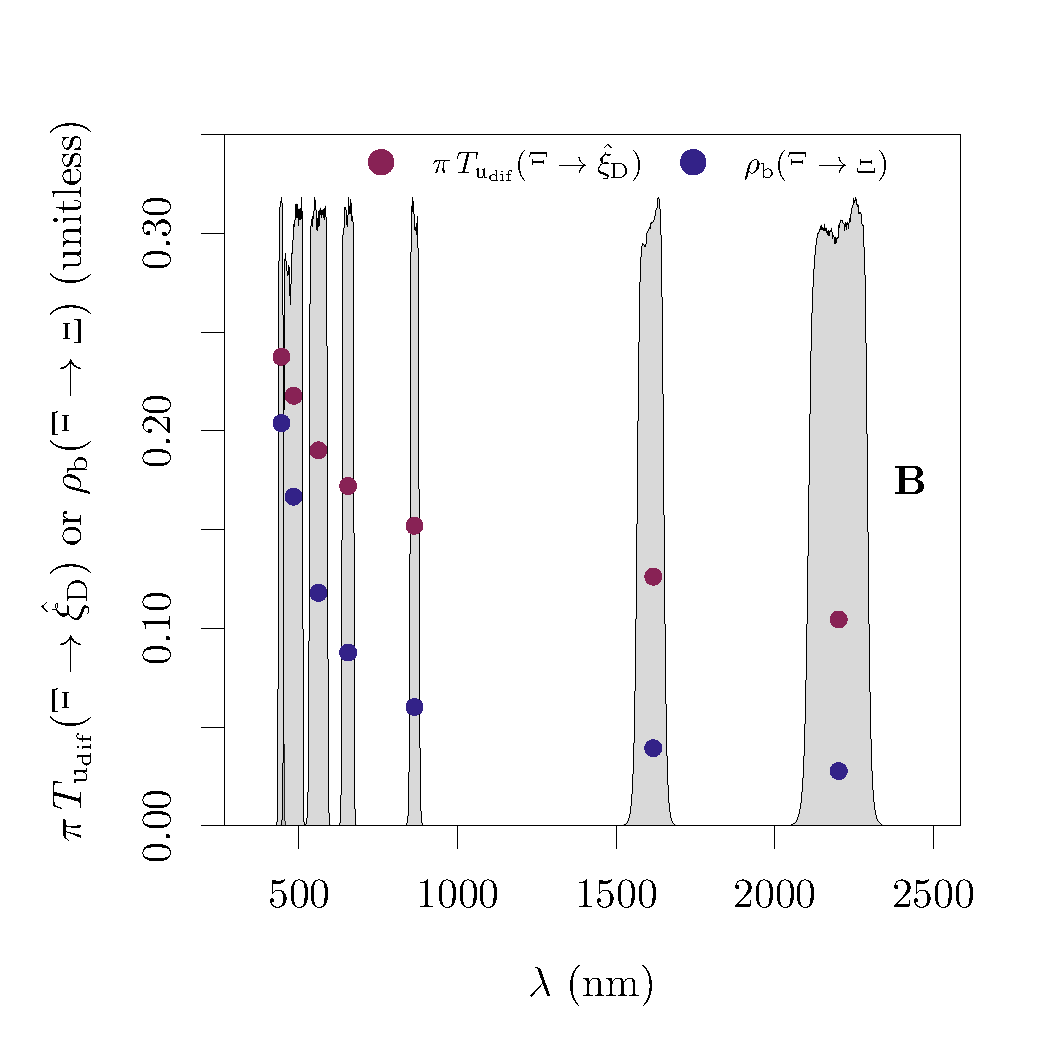
\includegraphics[trim={0 0.75cm 0 1cm},clip,width=\linewidth]{T_spectra_m.pdf}
    \end{subfigure}
   \caption{Selected atmospheric properties used in the simulations. Hemispherical-directional upward diffuse transmittance of the atmosphere toward the detector scaled by $\smash{\pi}$~sr, $\smash{\pi \, T_{\text{u}_\text{dif}}(\hemiup \rightarrow \hat{\xi}_\text{D})}$, and the spherical albedo, $\smash{\rho_\text{a}(\hemiup \rightarrow \hemidn)}$, for an atmosphere with continental aerosol model (A) or maritime aerosol model (B). $\smash{\tau_\text{aer}(865)=0.18}$ for both aerosol models. The grey polygons in the background show the relative spectral response functions of the first seven OLI wavebands.}
   \label{fig:sim01_atm_setup}
\end{figure}

The integro-normalised diffuse PSF, $\smash{\hat{\curlywedge}_\text{b}^*(\hemiup \rightarrow \hat{\xi}_\text{D}; \Lambda_w; \vec{x})}$, and the integro-normalised SAF, $\smash{\hat{\curlyvee}_{\text{b}}(\hemiup \rightarrow \hemidn; \Lambda_w; \vec{x})}$, were calculated using the same standard inputs as for 6SV in terms of atmospheric vertical profile, aerosol model and concentration. The resulting hemispherical-directional environmental reflectance for the upward diffuse transmittance, $\smash{\rho_{\text{s}_{\curlywedge_\text{b}^*}}(\hemidn \rightarrow \hat{\xi}_\text{D}; \Lambda_w; \vec{x})}$, and the bi-hemispherical environmental reflectance for the spherical albedo, $\smash{\rho_{\text{s}_{\curlyvee_\text{b}}}(\hemidn \rightarrow \hemiup; \Lambda_w; \vec{x})}$, for an $\smash{\tau_\text{aer}(865)}$ of 0.18~(unitless) are presented in Fig.~\ref{fig:sim01_env_averages}.

\begin{figure}[!htbp]
  \centering
    \begin{subfigure}[t]{0.48\textwidth}
      \centering
      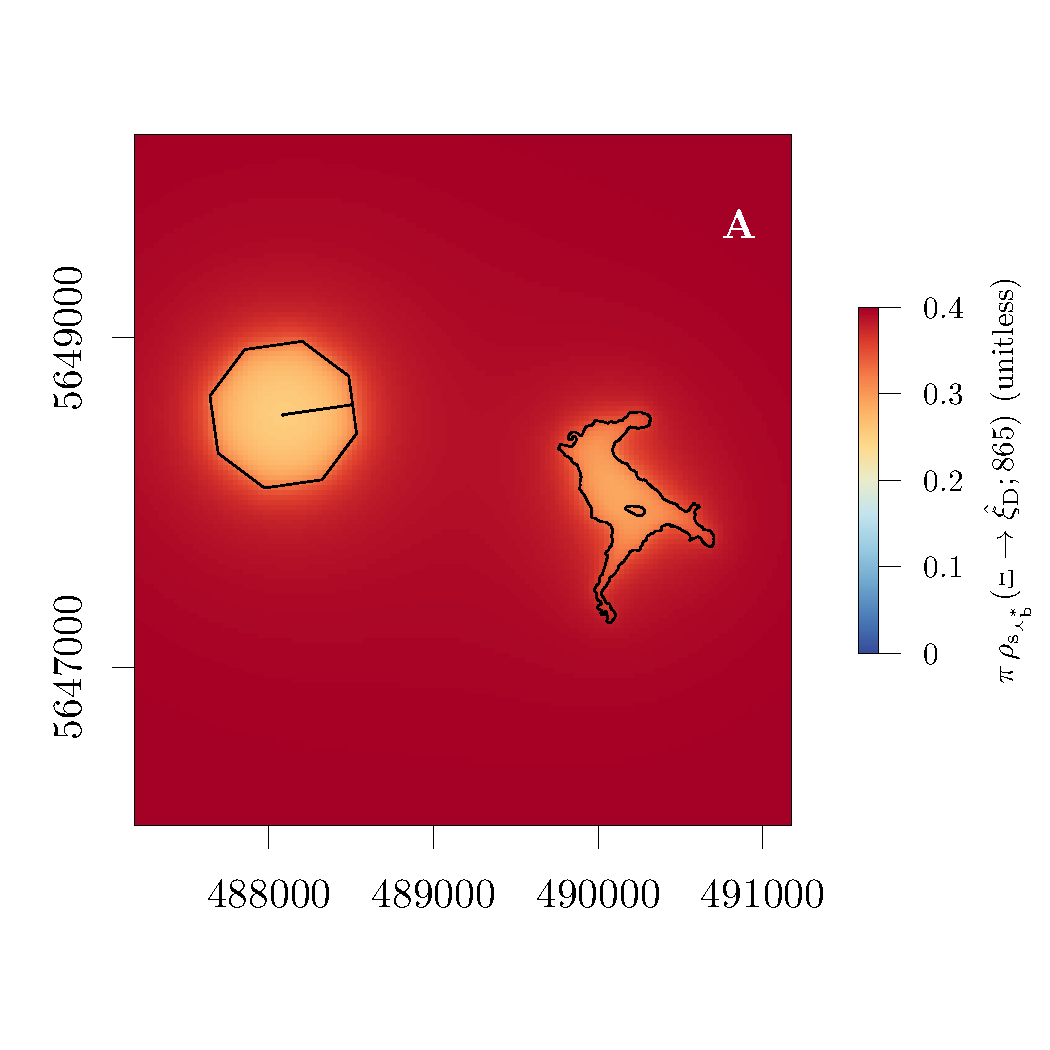
\includegraphics[trim={0 2cm 0 1cm},clip,width=\linewidth]{case_1_rho_env_psf_c.pdf}
    \end{subfigure}
    \begin{subfigure}[t]{0.48\textwidth}
      \centering
      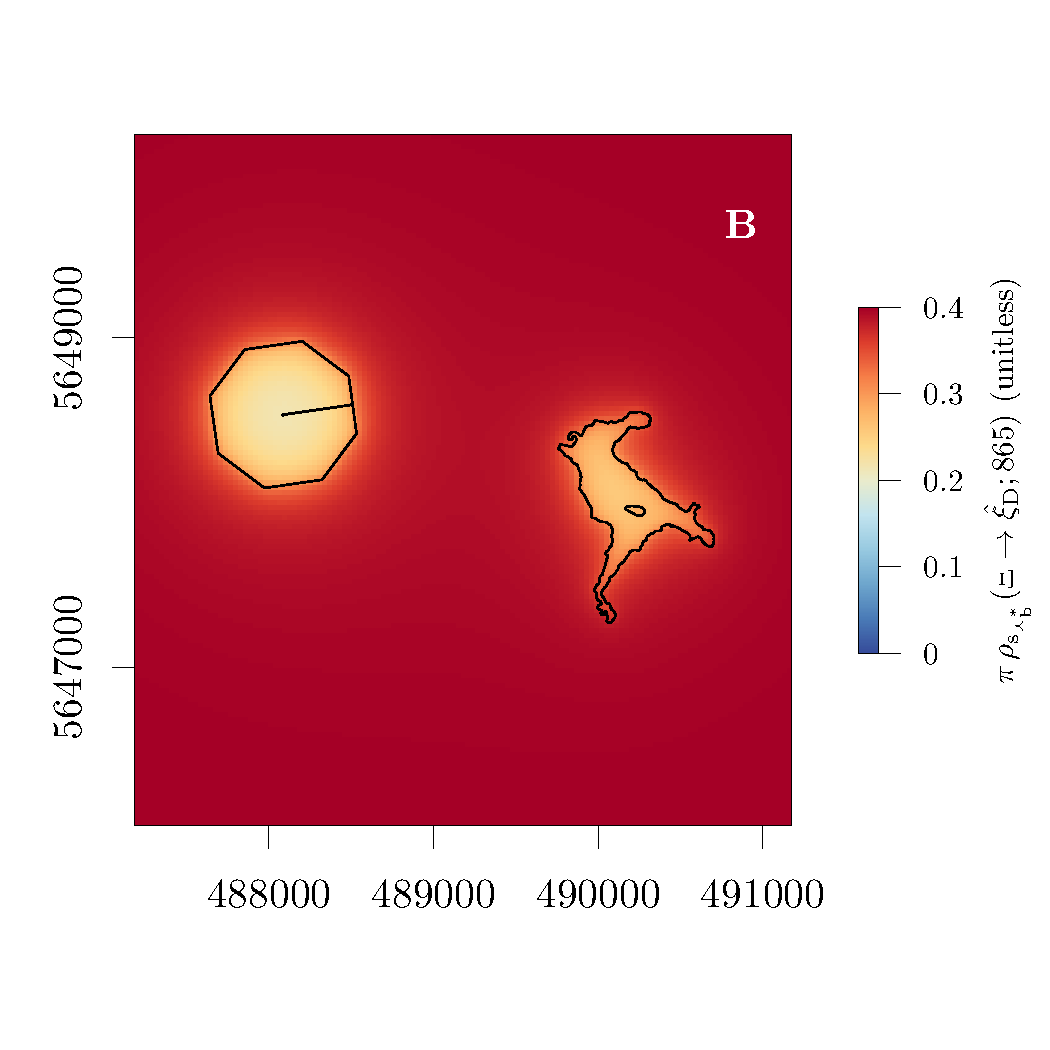
\includegraphics[trim={0 2cm 0 1cm},clip,width=\linewidth]{case_1_rho_env_psf_m.pdf}
    \end{subfigure}

    \begin{subfigure}[t]{0.48\textwidth}
      \centering
      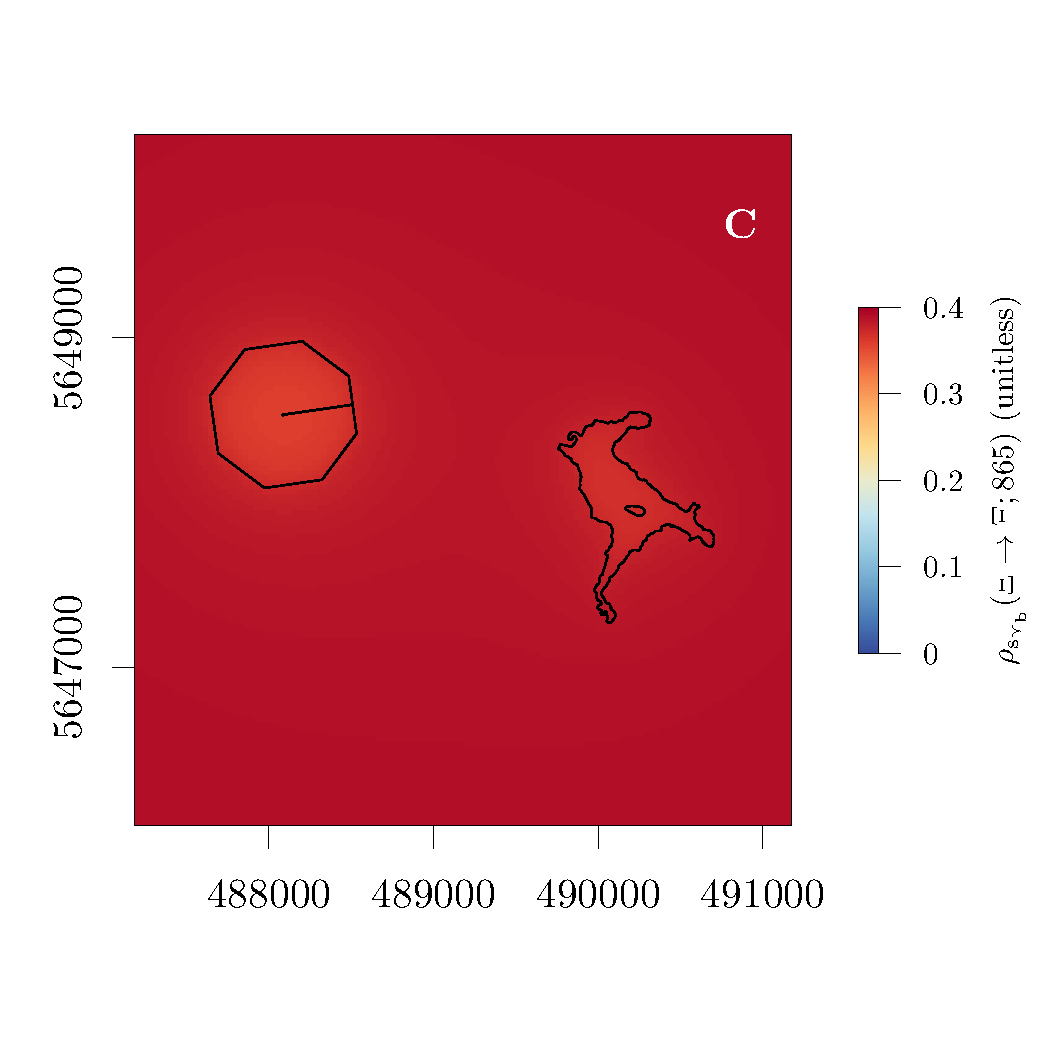
\includegraphics[trim={0 2cm 0 1cm},clip,width=\linewidth]{case_1_rho_env_sph_c.pdf}
    \end{subfigure}
    \begin{subfigure}[t]{0.48\textwidth}
      \centering
      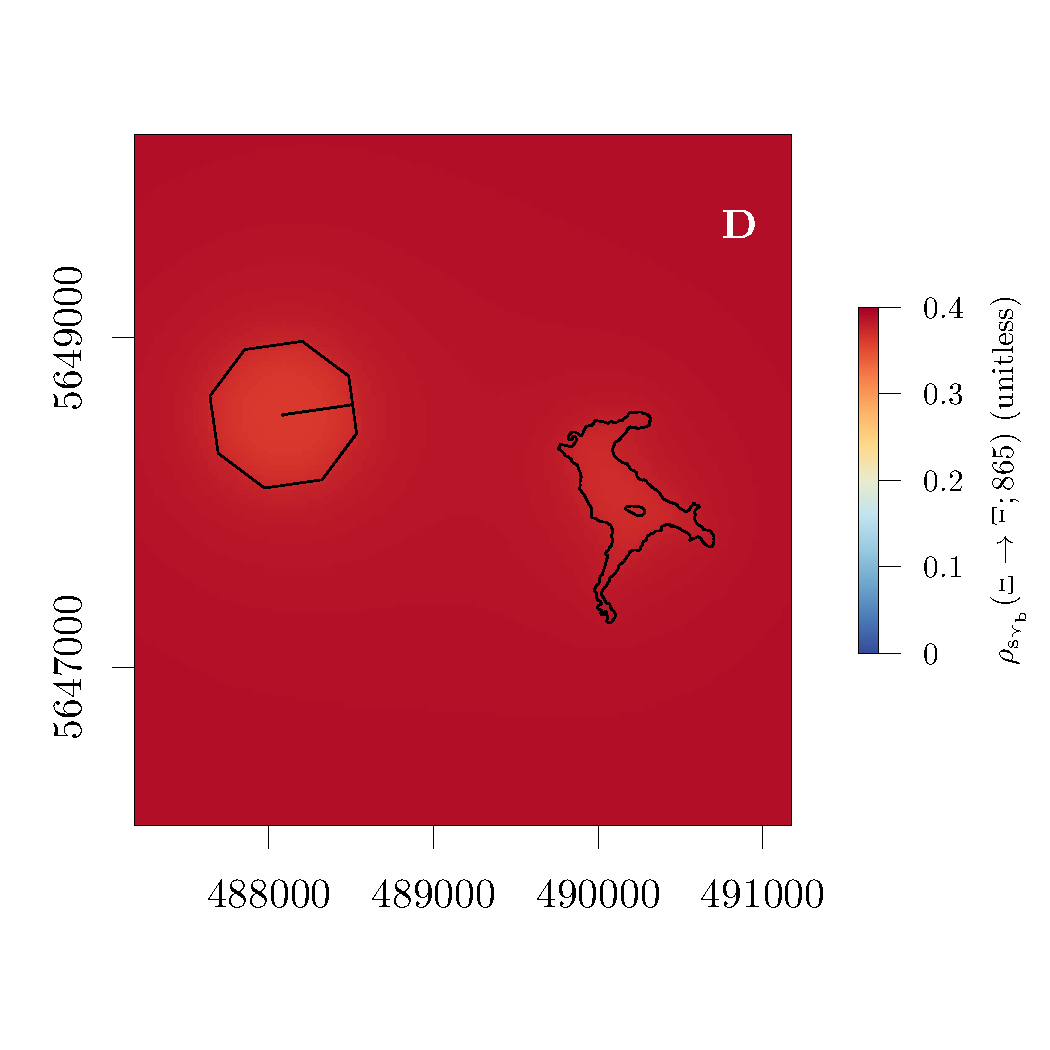
\includegraphics[trim={0 2cm 0 1cm},clip,width=\linewidth]{case_1_rho_env_sph_m.pdf}
    \end{subfigure}

   \caption{Environmental surface reflectances for an $\smash{\tau_\text{aer}(865)}$ of 0.18~(unitless). Hemispherical-directional environmental reflectance for the upward diffuse transmittance scaled by $\smash{\pi}$~sr, that is, the weighted average surface reflectance with weights given by $\smash{\hat{\curlywedge}_\text{b}(\hemiup \rightarrow \hat{\xi}_\text{D})}$, $\smash{\pi \, \rho_{\text{s}_{\curlywedge_\text{b}^*}}(\hemidn \rightarrow \hat{\xi}_\text{D})}$, for simulations with the continental aerosol model (A) and maritime aerosol model (B). Bi-hemispherical environmental reflectance for the spherical albedo, that is, the weighted average bi-hemispherical surface reflectance with weights given by $\smash{\hat{\curlyvee}_\text{b}(\hemiup \rightarrow \hemidn)}$, $\smash{\rho_{\text{s}_{\curlyvee_\text{b}}}(\hemidn \rightarrow \hemiup)}$, for simulations with the continental aerosol model (C) and maritime aerosol model (D). All variables presented for the NIR waveband of OLI, centred at wavelength 865~nm.}
   \label{fig:sim01_env_averages}
\end{figure}

In this chapter, the near-infrared waveband of OLI, centred at 865~nm, will be used to illustrate quantities and evaluate the performance of TSDSF and RAdCor, as it is the waveband with the highest reflectance contrast between the input spectra for water and vegetation (Fig.~\ref{fig:sim01_surf_setup}), while covering an atmospheric window with significant upward diffuse transmittance for both aerosol models (Fig.~\ref{fig:sim01_atm_setup}). For this reason, specific examples use a different $\smash{\tau_\text{aer}(550)}$ for each model, such as to result in the same $\smash{\tau_\text{aer}(865)}$.

\section{Evaluation of TSDSF}

The estimation of $\smash{\rho_\text{as}^\text{Hyp}(\hat{\xi}_0 \rightarrow \hat{\xi}_\text{D}; \Lambda_w; \vec{x})}$ from $\smash{\rho_\text{as}(\hat{\xi}_0 \rightarrow \hat{\xi}_\text{D}; \Lambda_w; \vec{x})}$ with Eq.~\ref{eq:est_rho_e_toa} is an important component to find the darkest pixels at the surface and to estimate $\smash{\tau_\text{aer}(550)}$ and aerosol model. To isolate the error of the approximation described in Eq.~\ref{eq:est_rho_e_toa} from other source of errors, we let the predefined $\smash{\tau_\text{aer}(550)}$ be equal to the $\smash{\tau_\text{aer}(550)}$ used in the simulations and use a large PSF radius (25~km). Fig.~\ref{fig:sim01_hyp_estimate} shows the ratio of the estimated function, $\smash{\rho_\text{as}^\text{Hyp Est.}}$, to the reference function, $\smash{\rho_\text{as}^\text{Hyp Ref.}}$, calculated with Eq.~\ref{eq:ret_rho_env_toa} for an $\smash{\tau_\text{aer}(865)}$ of 0.18~(unitless). For those example conditions, the maximum error in the estimation was $< 10$~\% for simulations with both aerosol models. 

\begin{figure}[!htbp]
  \centering
    \begin{subfigure}[t]{0.48\textwidth}
      \centering
      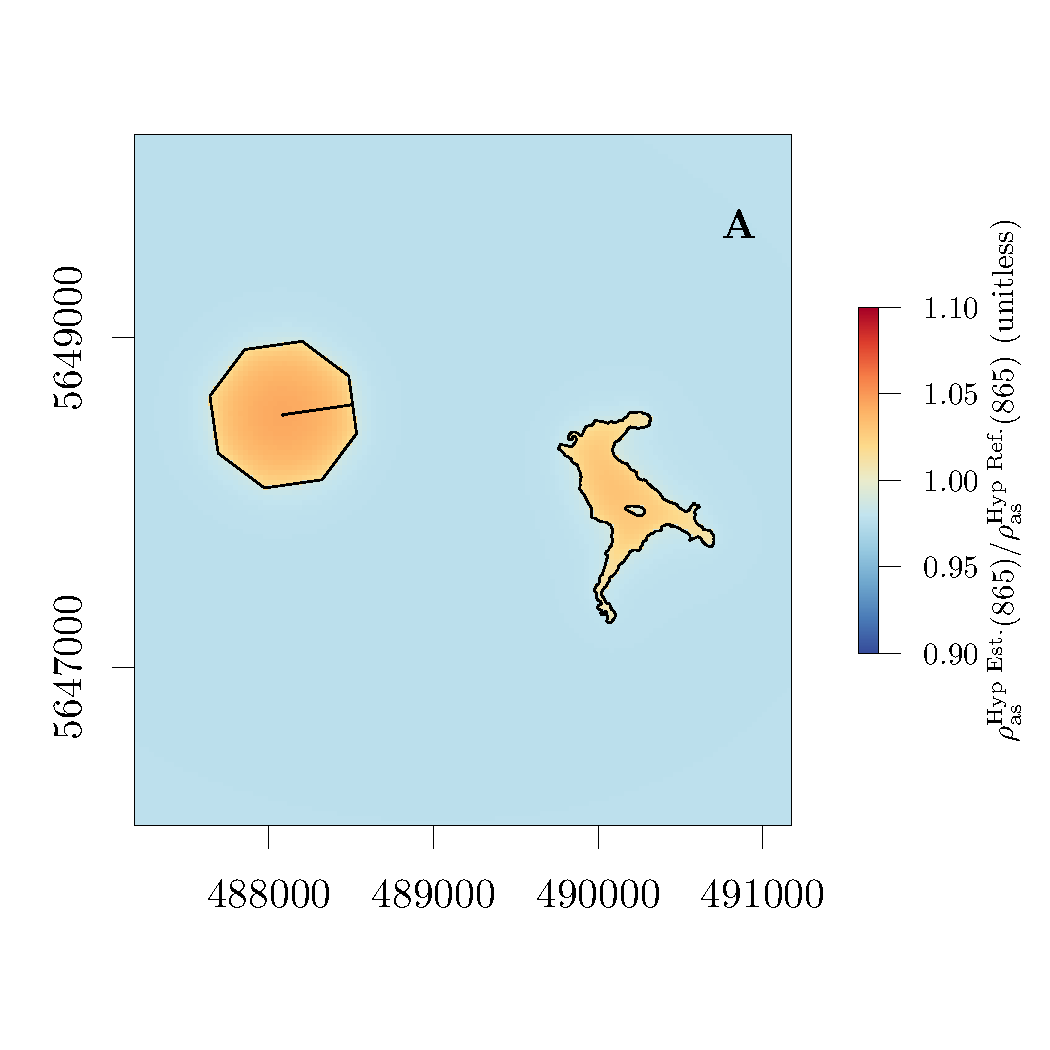
\includegraphics[trim={0 2cm 0 1cm},clip,width=\linewidth]{case_1_eval_rho_env_toa_c.pdf}
    \end{subfigure}
    \begin{subfigure}[t]{0.48\textwidth}
      \centering
      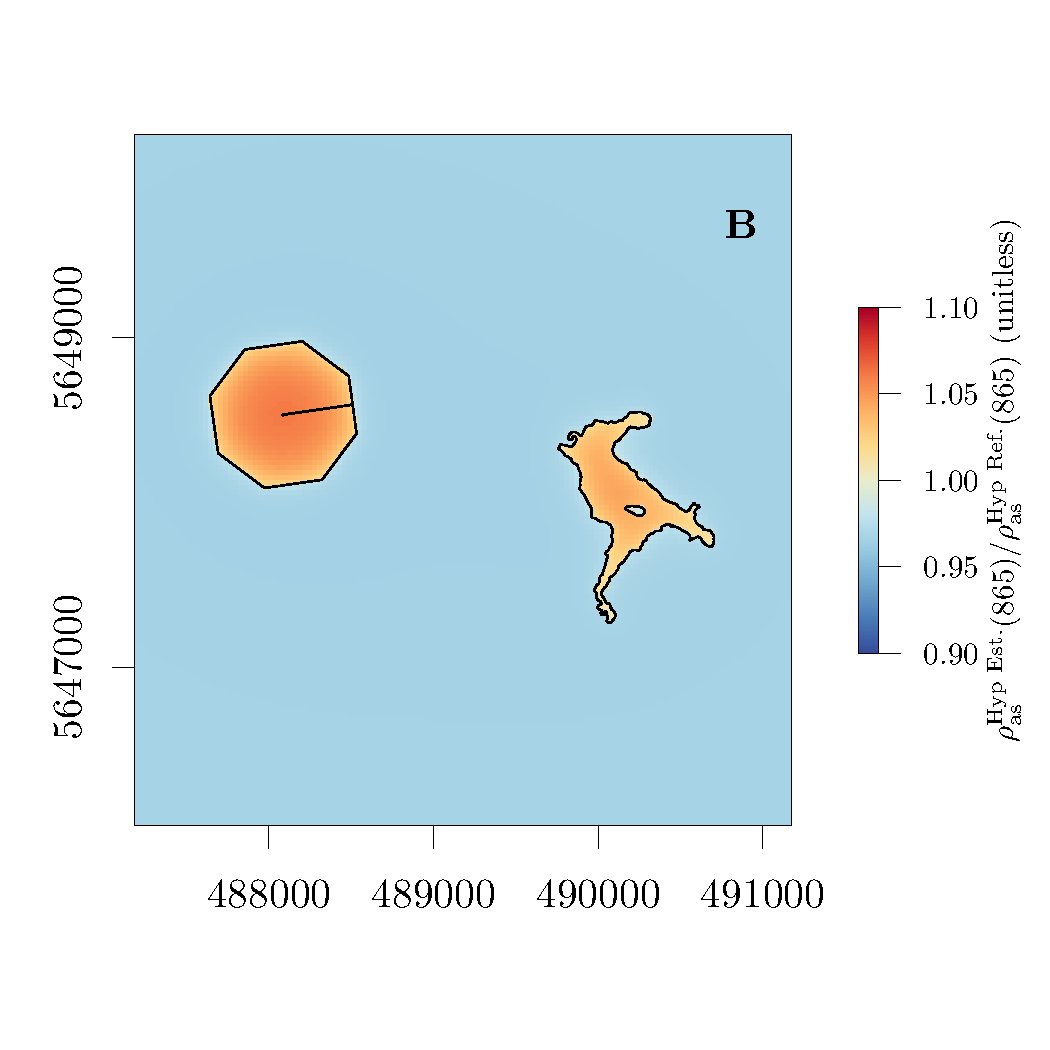
\includegraphics[trim={0 2cm 0 1cm},clip,width=\linewidth]{case_1_eval_rho_env_toa_m.pdf}
    \end{subfigure}
    
   \caption{Evaluation of the estimation of $\smash{\rho_\text{as}^\text{Hyp}(\hat{\xi}_0 \rightarrow \hat{\xi}_\text{D}; \Lambda_w; \vec{x})}$ from $\smash{\rho_\text{as}(\hat{\xi}_0 \rightarrow \hat{\xi}_\text{D}; \Lambda_w; \vec{x})}$. (A) Ratio of $\smash{\rho_\text{as}^\text{Hyp Est.}}$ to $\smash{\rho_\text{as}^\text{Hyp Ref.}}$ for the simulation with the continental aerosol model; (B) same as (A) but for the simulation with the maritime aerosol model. ``Est.'' stands for estimated value and ``Ref.'' stands for reference value.}
   \label{fig:sim01_hyp_estimate}
\end{figure}

In general the error of the approximation is positive (overestimation) over the darkest pixels, due to the further blurring of the observed signal resulting from the approximation in Eq.~\ref{eq:est_rho_e_toa}. The additional blurring also helps to explain the larger error observed for the estimation of $\smash{\rho_\text{as}^\text{Hyp}(\hat{\xi}_0 \rightarrow \hat{\xi}_\text{D}; \Lambda_w; \vec{x})}$ with the maritime aerosol model simulation. The diffuse PSF for the maritime aerosol model is more peaked than the diffuse PSF for the continental aerosol model (Fig.~\ref{fig:psf_sim_res}), resulting in a smaller degree of blurring for a given $\tau_\text{aer}(550)$. Any additional blurring will have a relatively higher impact for the maritime aerosol model simulation than for the one with the continental aerosol model. The sensitivity to the additional blurring is expected to increase with the increase in $\tau_\text{aer}(550)$, in part because it decreases the relative contribution of the Rayleigh diffuse PSF, increasing the kurtosis of the mixed diffuse PSF. In addition, Eq.~\ref{eq:est_rho_e_toa} is expected to be a valid approximation in conditions where the direct upward transmittance dominates the upward transmittance. Higher values of $\tau_\text{aer}(550)$ will therefore increase the error of the approximation.

The error of the $\smash{\rho_\text{as}^\text{Hyp}(\hat{\xi}_0 \rightarrow \hat{\xi}_\text{D}; \Lambda_w; \vec{x})}$ estimation over the darkest pixels will propagate to the $\tau_\text{aer}(550)$ and aerosol model estimation with the TSDSF. First it must be considered that though the simple scenario of this simulation leaves no ambiguity of the darkest pixels at the surface, the presence of error might lead to less optimal selection of darkest surface pixels in real scenes. Further, an overestimation as seen in Fig.~\ref{fig:sim01_hyp_estimate} will lead to an underestimation $\tau_\text{aer}(550)$ for a given aerosol model. As shown in Eq.~\ref{eq:ret_ratio}, the path corrected ratio $\smash{\rho_\text{pc} / \rho_\text{pc}^\text{Hyp}}$ over the darkest pixels is equal to the diffuse fraction of the upward transmittance. Therefore, an overestimation of $\smash{\rho_\text{as}^\text{Hyp}(\hat{\xi}_0 \rightarrow \hat{\xi}_\text{D}; \Lambda_w; \vec{x})}$ over the darkest pixels will reduce the ratio, resulting in a lower diffuse fraction and a lower estimation of $\tau_\text{aer}(550)$.

We evaluate the propagated uncertainty through TSDSF using the $\tau_\text{aer}(550)$ estimation error as a metric. First we evaluate the impact of different predefined values of $\tau_\text{aer}(550)$, isolating it from errors related to the finite PSF by using a large PSF radius~(25 km). The results, presented in Fig.~\ref{fig:sim01_tsdsf_all_aot}, for a wide range of reference and predefined $\tau_\text{aer}(550)$ show two main patterns: (1) There is an overall tendency of underestimation of $\tau_\text{aer}(550)$ which is proportional to the $\tau_\text{aer}(550)$ used in the simulation. (2) The estimation improves for all simulated $\tau_\text{aer}(550)$ for larger values of predefined $\tau_\text{aer}(550)$. Further, in specific circumstances, TSDSF estimates the incorrect aerosol model for maritime aerosol simulations, resulting also in larger errors in $\tau_\text{aer}(550)$ estimation.

\begin{figure}[!htbp]
  \centering
    \begin{subfigure}[t]{0.48\textwidth}
      \centering
      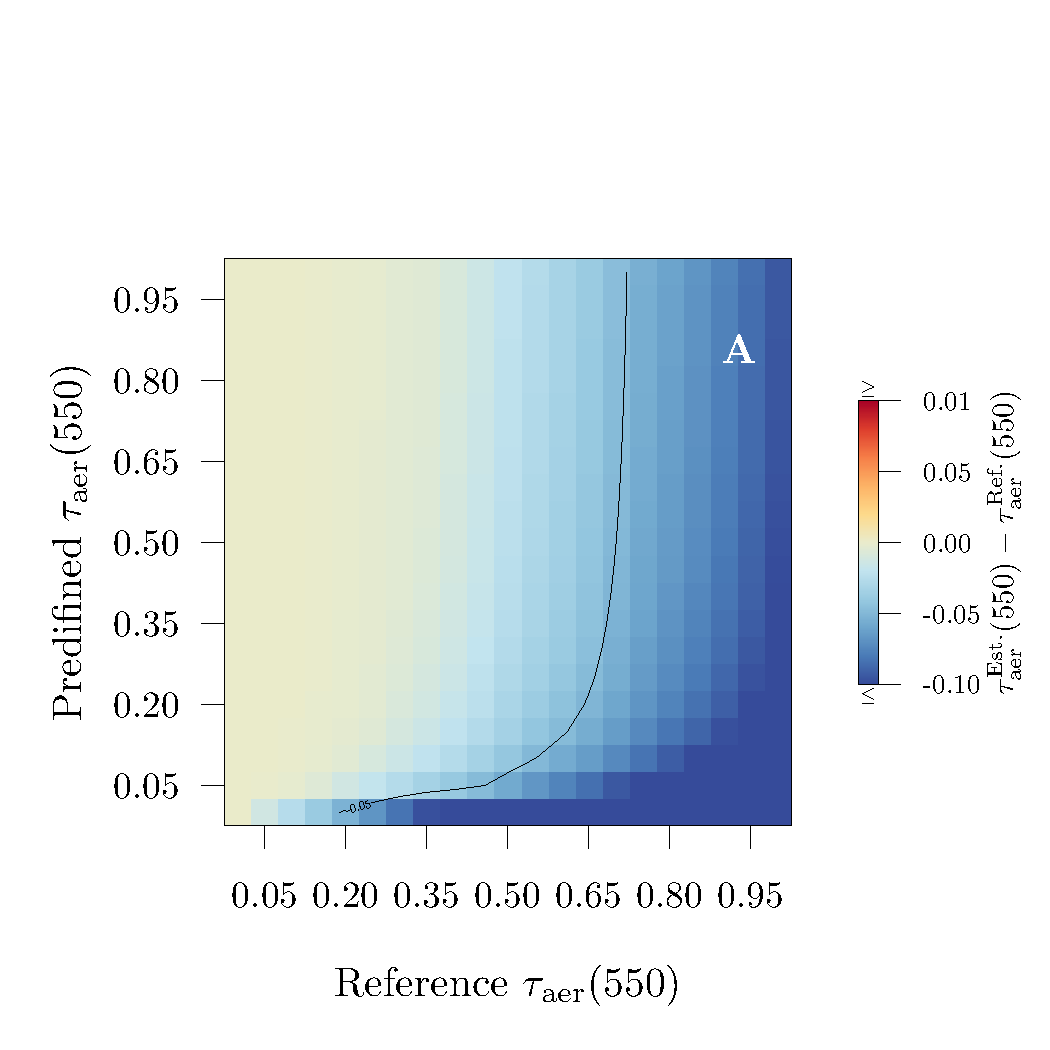
\includegraphics[trim={0 0.75cm 0 1cm},clip,width=\linewidth]{case_1_eval_ts_dsf_aot_c.pdf}
    \end{subfigure}
    \begin{subfigure}[t]{0.48\textwidth}
      \centering
      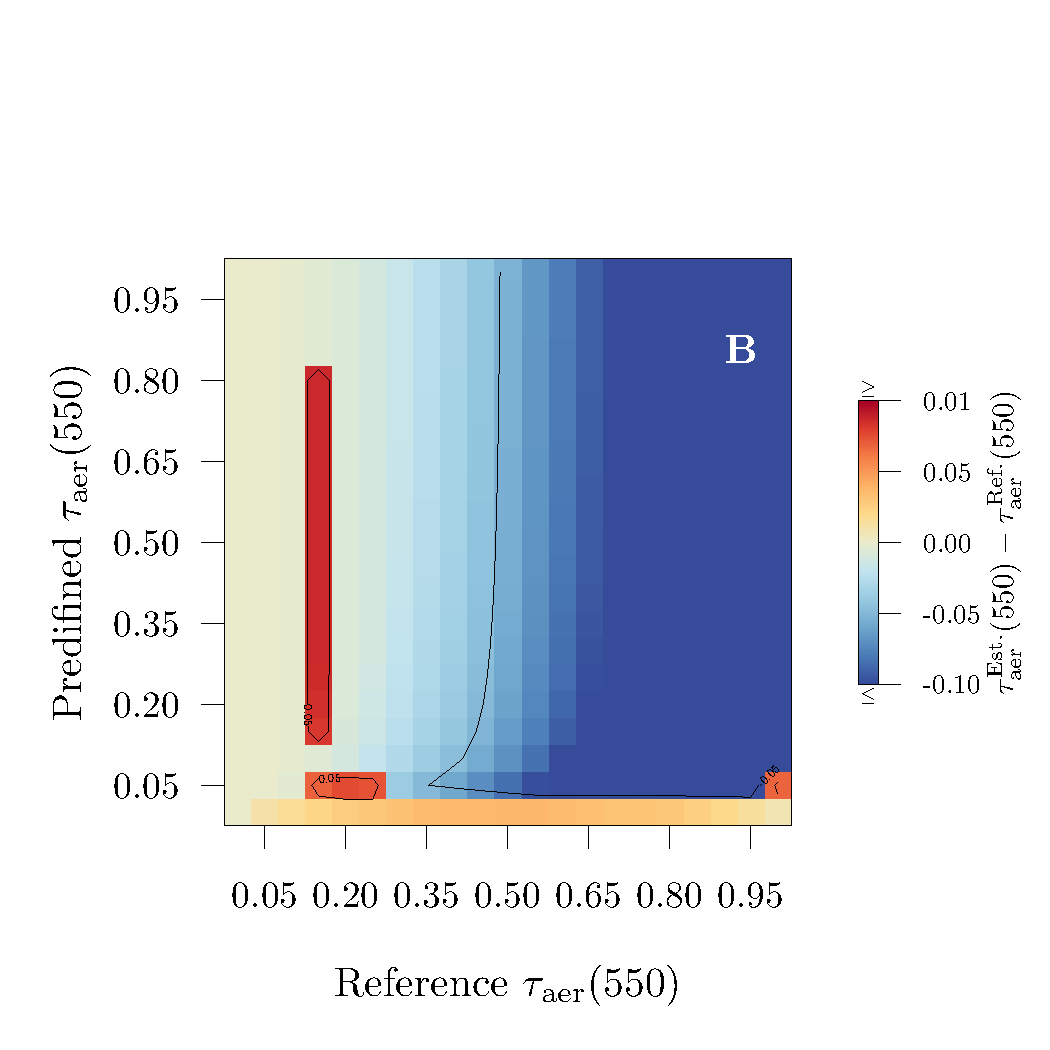
\includegraphics[trim={0 0.75cm 0 1cm},clip,width=\linewidth]{case_1_eval_ts_dsf_aot_m.pdf}
    \end{subfigure}
   \caption{TSDSF estimation error of $\tau_\text{aer}(550)$. $\tau_\text{aer}(550)$ estimation error for simulations with the continental aerosol model (A) and the maritime aerosol model (B). The X-axis provides the $\tau_\text{aer}(550)$ used in the simulation, while the Y-axis provides the $\tau_\text{aer}(550)$ used for the TSDSF estimation.}
   \label{fig:sim01_tsdsf_all_aot}
\end{figure}

The errors in the estimation of $\smash{\rho_\text{as}^\text{Hyp}(\hat{\xi}_0 \rightarrow \hat{\xi}_\text{D}; \Lambda_w; \vec{x})}$ discussed previously seem to explain the observed error patterns in $\tau_\text{aer}(550)$ retrieval. The degrading performance of TSDSF with increase in the simulated $\tau_\text{aer}(550)$ is intrinsic to the TSDSF approach, as the approximation used to estimate the hypothetical quantity is expected to hold only for conditions in which the direct fraction dominates the upward transmittance. The improvement of estimation with larger predefined $\tau_\text{aer}(550)$ implies that the further blurring caused by the convolution of $\smash{\rho_\text{as}(\hat{\xi}_0 \rightarrow \hat{\xi}_\text{D}; \Lambda_w; \vec{x})}$ with the predefined PSF is minimised by reducing the relative contribution of the Rayleigh PSF. This suggests that the approximation of Eq.~\ref{eq:est_rho_e_toa} can be improved by using only the aerosol diffuse PSF, that is, without the Rayleigh contribution. The worse performance of $\tau_\text{aer}(550)$ retrievals for the simulations with the maritime aerosol model are again a consequence of the higher sensitivity to further blurring in the estimation of $\smash{\rho_\text{as}^\text{Hyp}(\hat{\xi}_0 \rightarrow \hat{\xi}_\text{D}; \Lambda_w; \vec{x})}$, as it has a higher diffuse fraction of the upward diffuse transmittance for a given $\tau_\text{aer}(550)$ value. Nonetheless, considering that the observed average $\tau_\text{aer}(550)$ is typically $< 0.3$ over most of the globe, TSDSF should provide appropriate estimates for most scenes.

The effect of the PSF extent on the TSDSF estimation was isolated by using the best predefined $\tau_\text{aer}(550)$ from the previous analysis, 1 (unitless), and evaluated by performing the TSDSF approach over a range of PSF radius from 2.5~km to 25~km. Fig.~\ref{fig:sim01_tsdsf_all_psf} shows that the $\tau_\text{aer}(550)$ estimation error is largely independent of PSF extent. The lack of sensitivity of TSDSF to the PSF radius likely results from the high coverage of the diffuse PSF when using only the PSF for aerosols (high predefined $\tau_\text{aer}(550)$). A PSF radius of 5~km covers $> 90$~\% of the diffuse transmittance for both aerosol models (Fig.~\ref{fig:psf_sim_res}). This observation can be exploited by employing a shorter PSF extent to reduce the computations for TSDSF. In addition, a shorter PSF extent resulting in lower coverage can be exploited to partially compensate for the further blurring in the estimation of $\smash{\rho_\text{as}^\text{Hyp}(\hat{\xi}_0 \rightarrow \hat{\xi}_\text{D}; \Lambda_w; \vec{x})}$, by re-normalising the truncated diffuse PSF instead of complementing the missing signal with the local average (\textit{cf.} Chapter~\ref{ch:finite}). 

\begin{figure}[!htbp]
  \centering
    \begin{subfigure}[t]{0.48\textwidth}
      \centering
      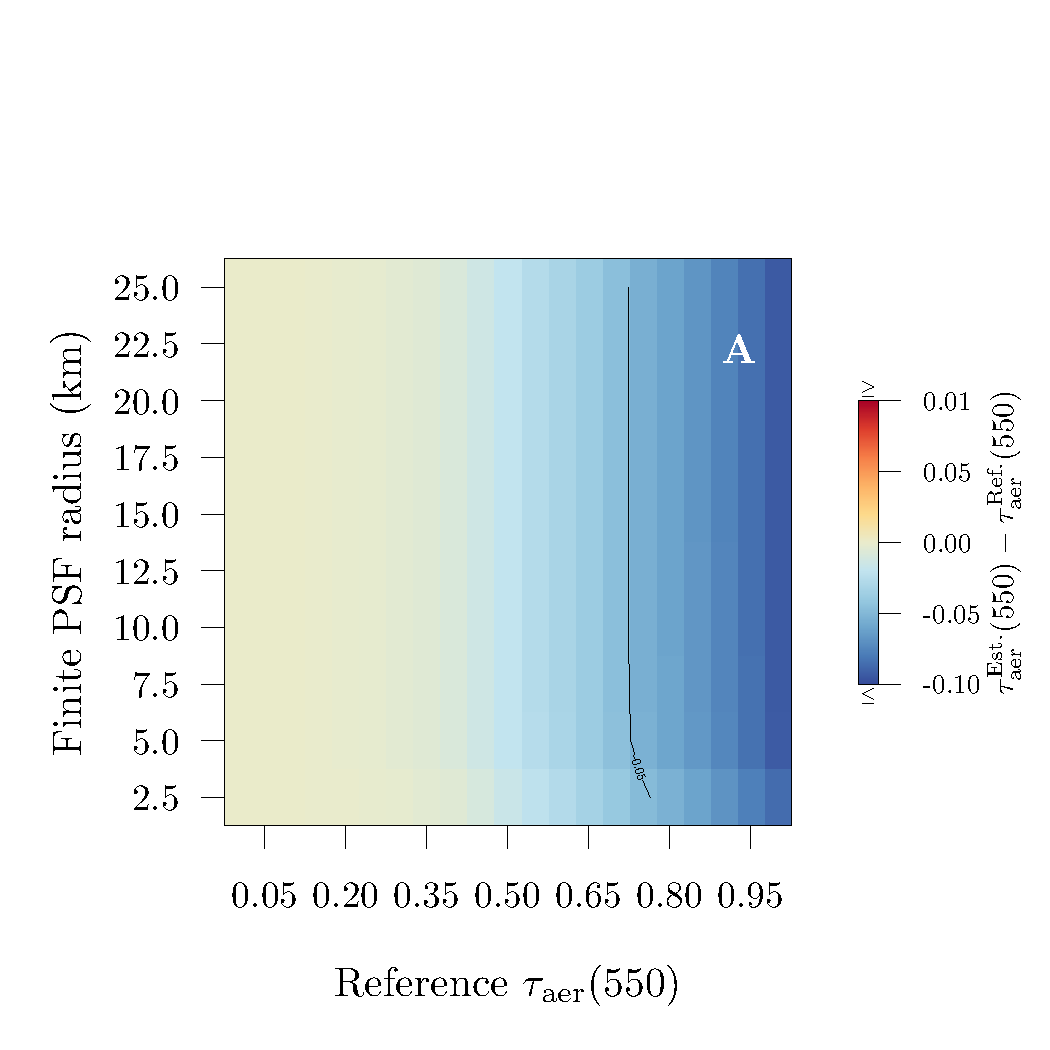
\includegraphics[trim={0 0.75cm 0 1cm},clip,width=\linewidth]{case_1_eval_ts_dsf_psf_c.pdf}
    \end{subfigure}
    \begin{subfigure}[t]{0.48\textwidth}
      \centering
      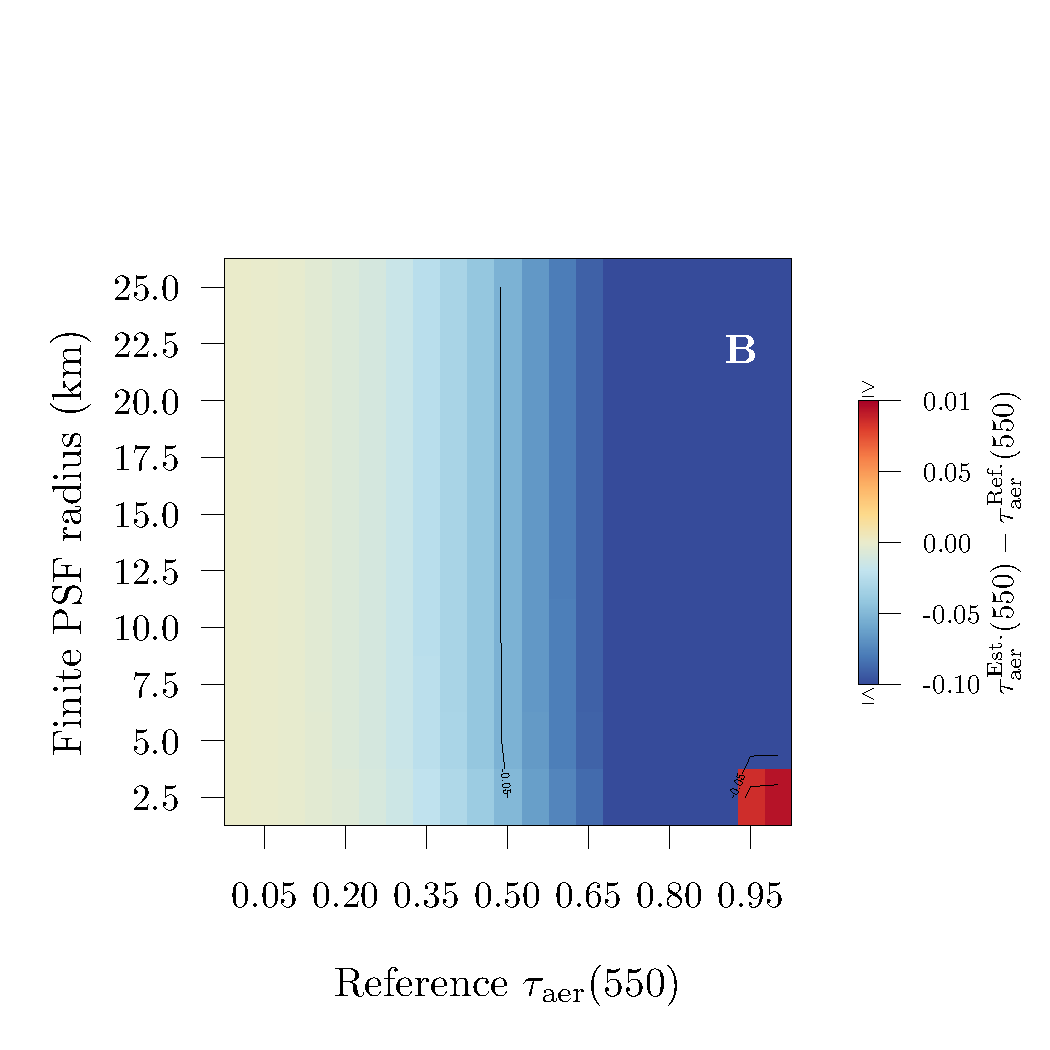
\includegraphics[trim={0 0.75cm 0 1cm},clip,width=\linewidth]{case_1_eval_ts_dsf_psf_m.pdf}
    \end{subfigure}
   \caption{TSDSF estimation error of $\tau_\text{aer}(550)$. $\tau_\text{aer}(550)$ estimation error for simulations with the continental aerosol model (A) and the maritime aerosol model (B). The X-axis provides the $\tau_\text{aer}(550)$ used in the simulation, while the Y-axis provides the PSF extent used for the TSsDSF estimation.}
   \label{fig:sim01_tsdsf_all_psf}
\end{figure}

\section{Evaluation of RAdCor}

With the estimated aerosol model and concentration, the optical functions of the atmosphere can be calculated. These, together with the estimation of $\smash{\rho_{\text{s}_{\curlyvee_\text{b}}}(\hemidn \rightarrow \hemiup; \Lambda_w; \vec{x})}$, can be plugged in to Eq.~\ref{eq:radcor_lambertian_scene_fourier_finite} to retrieve $\smash{\rho_\text{s}(\hemidn \rightarrow \hat{\xi}_\text{D}; \Lambda_W; \vec{x})}$. 

The approximations required to estimate $\smash{\rho_{\text{s}_{\curlyvee_\text{b}}}(\hemidn \rightarrow \hemiup; \Lambda_w; \vec{x})}$ are evaluated directly by setting the aerosol model and $\tau_\text{aer}(550)$ to the same values used in the simulation, and by using a PSF extent of 25~km. Fig.~\ref{fig:sim01_env_sph_est} shows an example for the simulations with $\tau_\text{aer}(550) = 0.3$ (unitless). Despite the approximations necessary to estimate $\smash{\rho_{\text{s}_{\curlyvee_\text{b}}}(\hemidn \rightarrow \hemiup; \Lambda_w; \vec{x})}$ from the TOA signal, the blurring caused by the SAF is dominant, allowing for the use of the homogeneous surface reflectance framework and resulting in a small error to the reference value. We note, however, that $\smash{\rho_{\text{s}_{\curlyvee_\text{b}}}(\hemidn \rightarrow \hemiup; \Lambda_w; \vec{x})}$ is that for the first order of the surface-atmosphere interaction.

\begin{figure}[!htbp]
  \centering
    \begin{subfigure}[t]{0.48\textwidth}
      \centering
      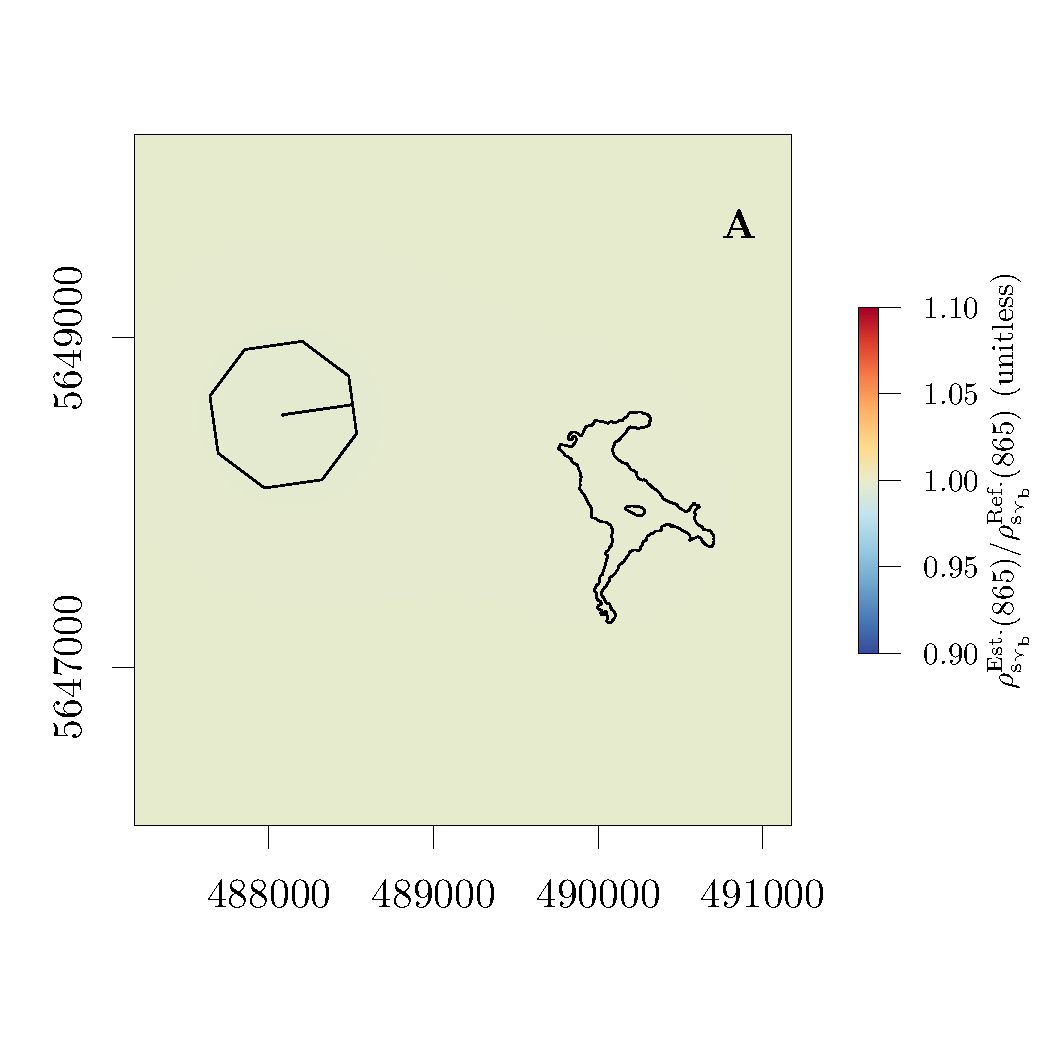
\includegraphics[trim={0 2cm 0 1cm},clip,width=\linewidth]{case_1_eval_rho_env_sph_c_est.pdf}
    \end{subfigure}
    \begin{subfigure}[t]{0.48\textwidth}
      \centering
      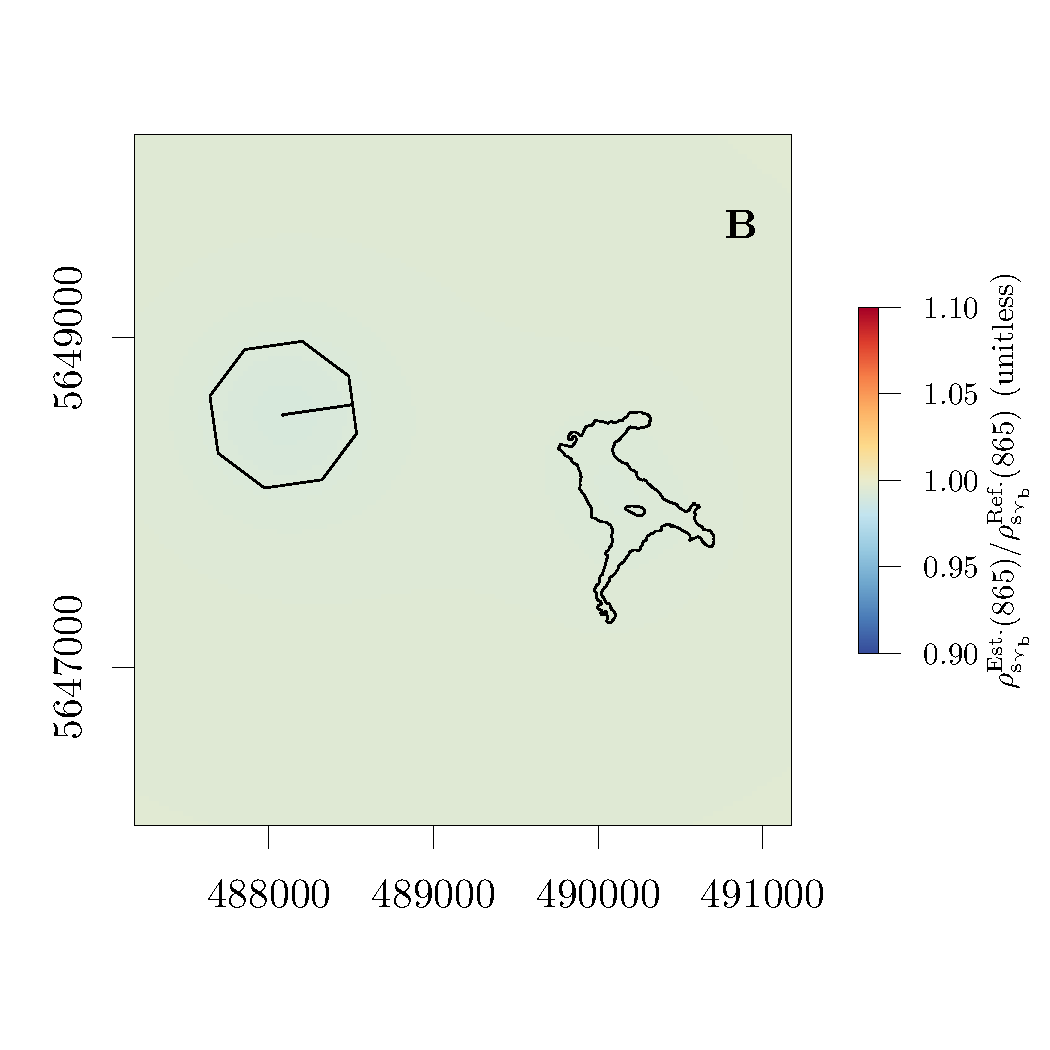
\includegraphics[trim={0 2cm 0 1cm},clip,width=\linewidth]{case_1_eval_rho_env_sph_m_est.pdf}
    \end{subfigure}
   \caption{Evaluation of the $\smash{\rho_{\text{s}_{\curlyvee_\text{b}}}(\hemidn \rightarrow \hemiup; \Lambda_w; \vec{x})}$ estimate against the reference value calculated with Eq.~\ref{eq:theory_bhem} for the OLI waveband centered at 865~nm. (A) Ratio for the Continental model simulation; (B) Ratio for the Maritime model simulation.}
   \label{fig:sim01_env_sph_est}
\end{figure}

The final critical step for the retrieval of the surface reflectance is the selection of the finite PSF extent within the constraints possible for a given scene extent (\textit{cf.} Chapter~\ref{ch:finite}). The missing fraction of the diffusely transmitted signal has to be accounted for by an estimated value, with the default in RAdCor being the local average. Therefore, the error in the correction will be proportional to the PSF extent. We isolate the effect of the PSF extent by performing the atmospheric correction using the reference $\tau_\text{aer}(550)$ and aerosol model, an evaluate the retrieval over a range of PSF radius. Fig.~\ref{fig:sim01_radcor_all} shows the average surface reflectance estimation error over the Blankaart reservoir. As expected, there is an improvement in the retrievals with larger PSF radius, with the lower boundary dependent on the $\tau_\text{aer}(550)$ used in the simulation. 

The results suggests that the largest possible PSF extent, to a maximum of 25~km, should be used for the retrieval of surface reflectance. This value, however, will be constrained by the scene size. As an example, for a centre scene area of 7~km, a PSF radius of 25~km requires a scene extent of 57~km. For targets close to the edge of the sensor swath and for commercial very high spatial resolution imagery, shorter PSF extents will be necessary, resulting in larger estimation errors.

We note, however, that the need for large kernel extents was not supported by the preliminary validation with real imagery. While other insights provided by the simulation were useful in improving the processor, kernel radius as low as 5~km or 3.5~km gave similar results to larger kernels.  

\begin{figure}[!htbp]
  \centering
    \begin{subfigure}[t]{0.48\textwidth}
      \centering
      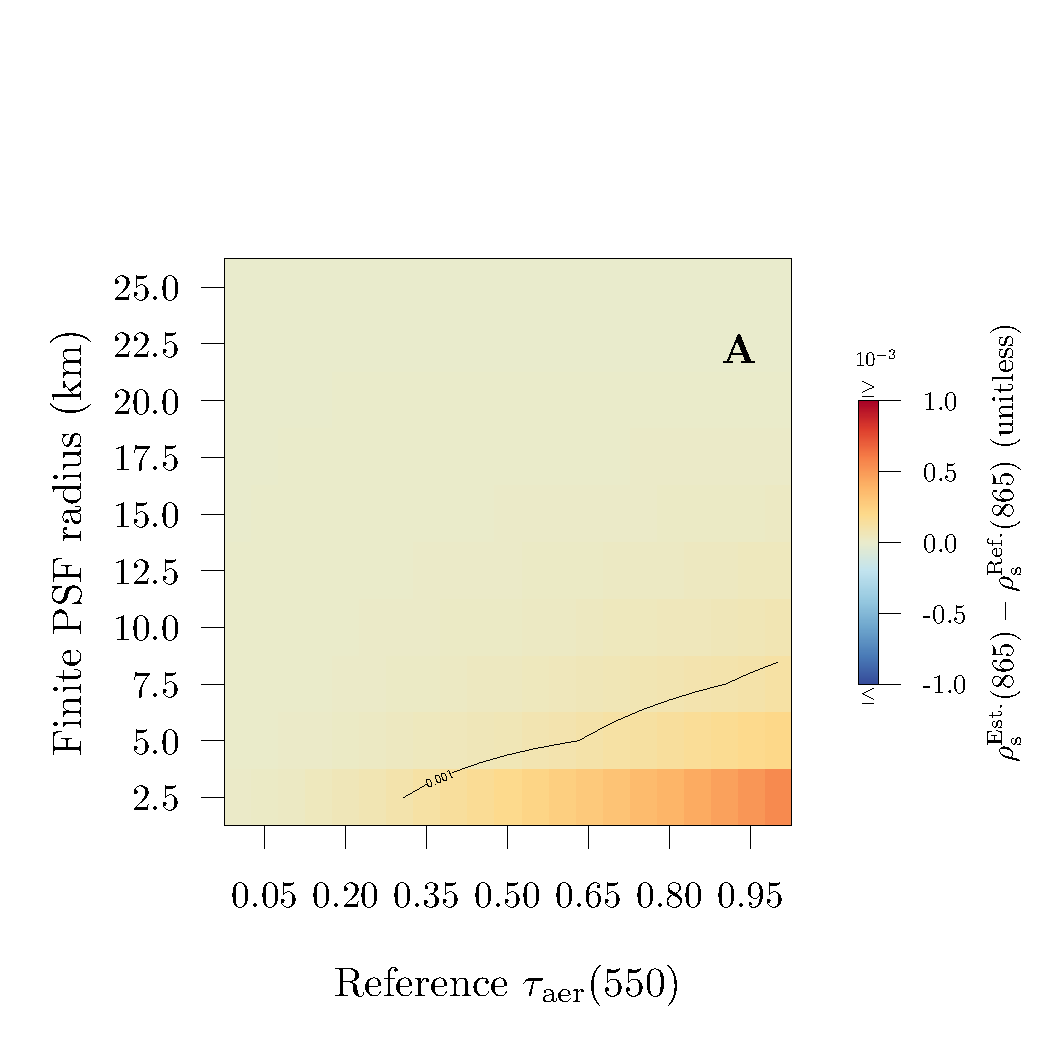
\includegraphics[trim={0 0.75cm 0 2.2cm},clip,width=\linewidth]{case_1_eval_radcor_abs_c}
    \end{subfigure}
    \begin{subfigure}[t]{0.48\textwidth}
      \centering
      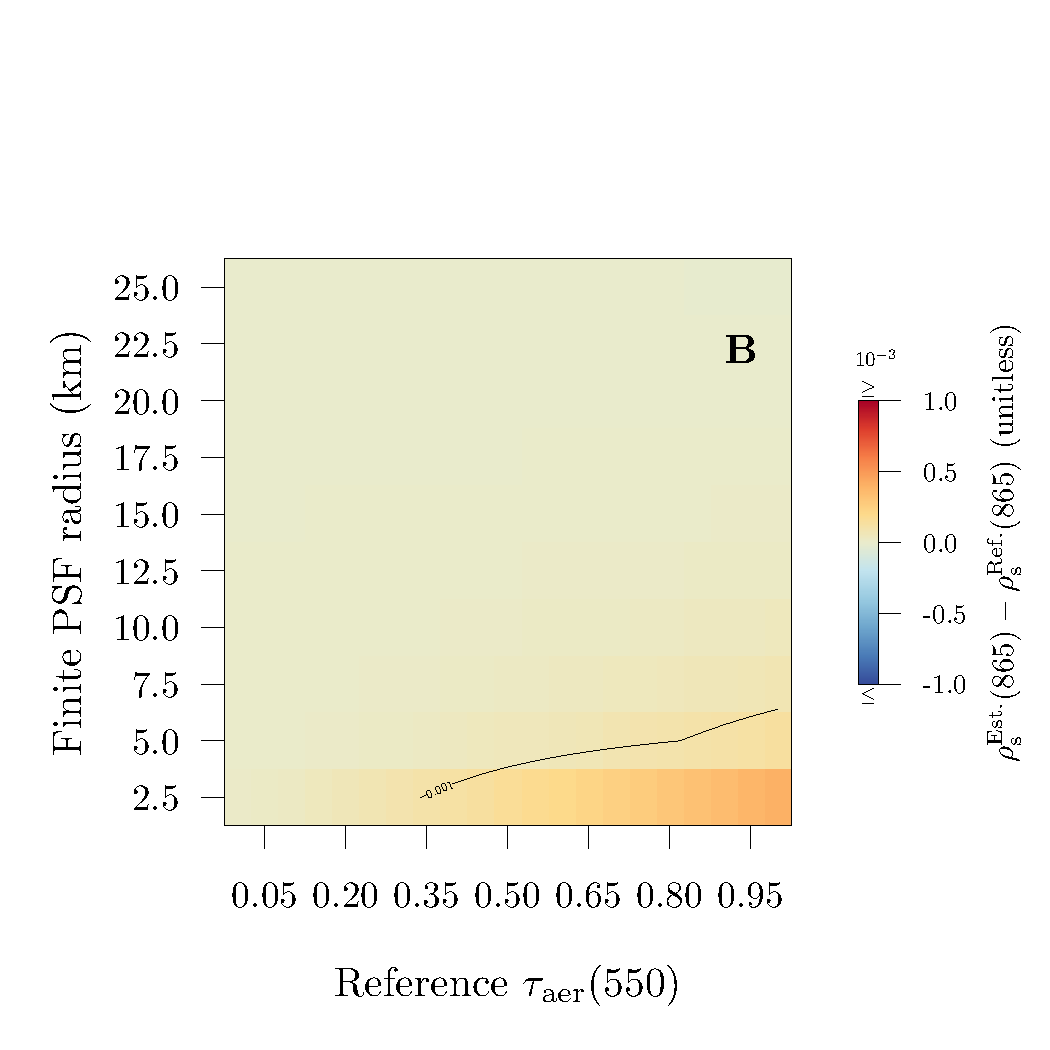
\includegraphics[trim={0 0.75cm 0 2.2cm},clip,width=\linewidth]{case_1_eval_radcor_abs_m}
    \end{subfigure}
    
    \begin{subfigure}[t]{0.48\textwidth}
      \centering
      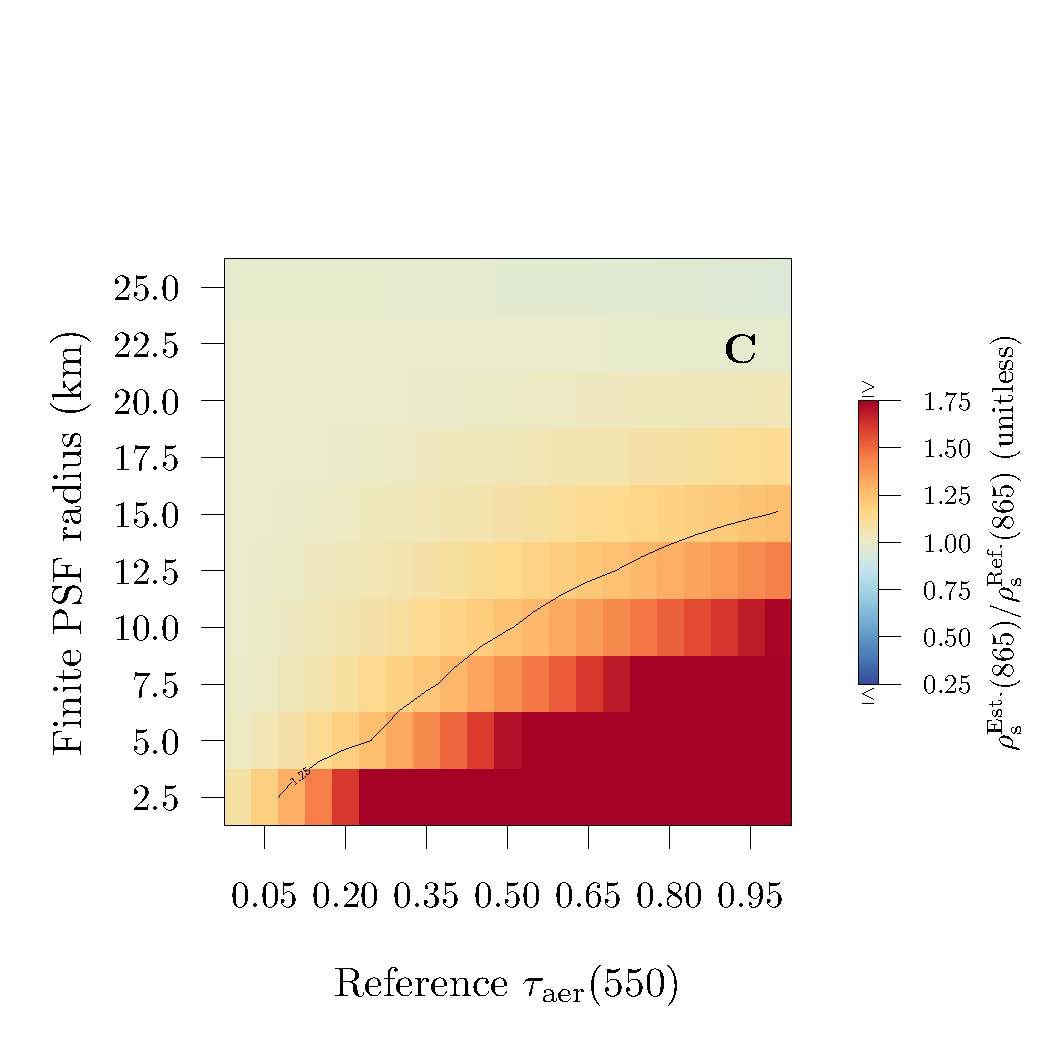
\includegraphics[trim={0 0.75cm 0 2.2cm},clip,width=\linewidth]{case_1_eval_radcor_rel_c}
    \end{subfigure}
    \begin{subfigure}[t]{0.48\textwidth}
      \centering
      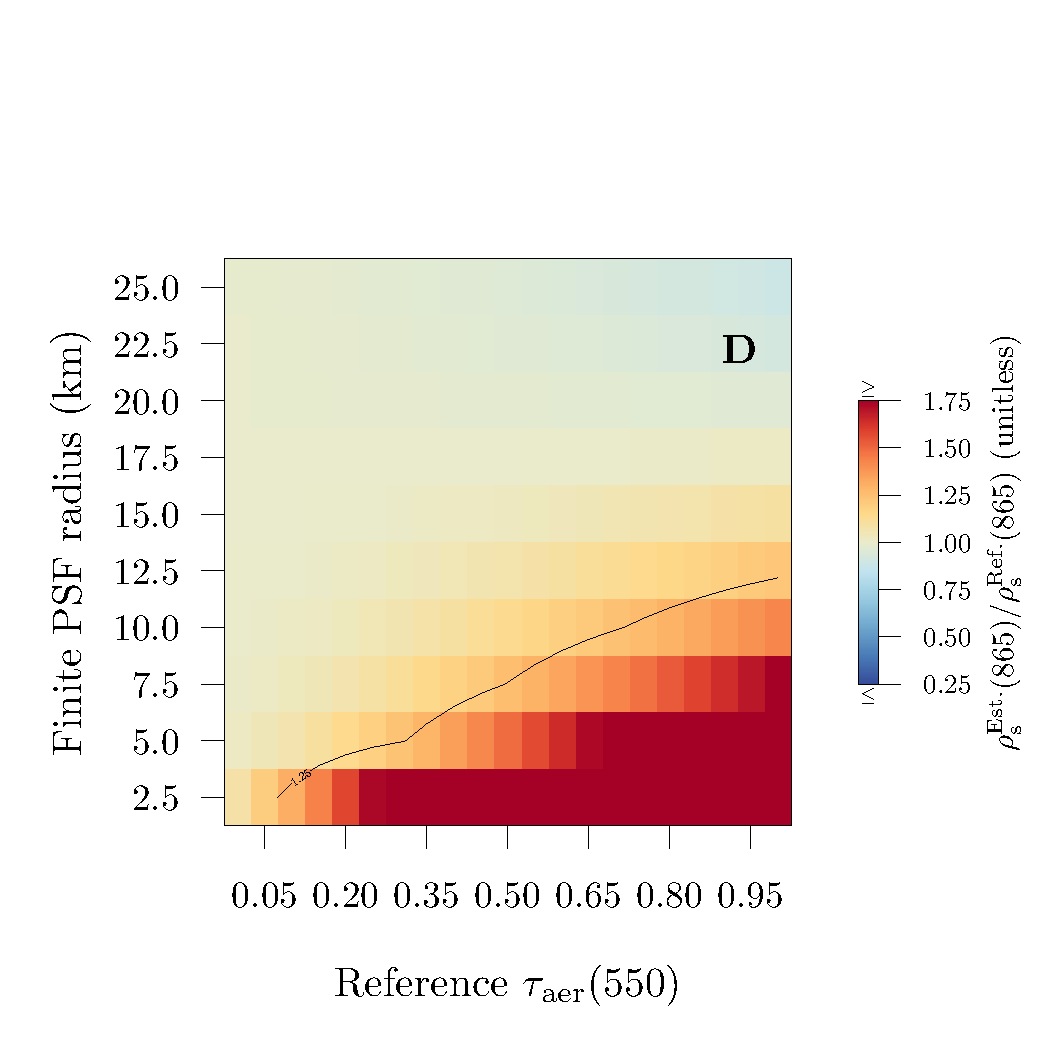
\includegraphics[trim={0 0.75cm 0 2.2cm},clip,width=\linewidth]{case_1_eval_radcor_rel_m}
    \end{subfigure}

   \caption{Evaluation of atmospheric correction over the Blankaart reservoir for different finite PSF radius. Difference between the average estimated surface reflectance and the reference reflectance for the continental model simulations (A) and maritime model simulations (B). Ratio of the average estimated surface reflectance and the reference reflectance for the continental model simulations (C) and maritime model simulations (D). The reference $\tau_\text{aer}(550)$ for each simulation was used for the correction.}
   \label{fig:sim01_radcor_all}
\end{figure}

\section{Combined evaluation of TSDSF and RAdCor}

In the previous section, RAdCor was evaluated in absence of errors in the estimation of aerosol model and $\tau_\text{aer}(550)$. Here, the aerosol properties used for the correction are taken from the TSDSF estimation. The impact of the underestimation of $\tau_\text{aer}(550)$ can be clearly seen in Fig.~\ref{fig:sim01_full_eval}. In absence of errors in $\tau_\text{aer}(550)$ estimation, the retrieved surface reflectance for the maritime aerosol model has better performance than for the continental aerosol model (Fig.~\ref{fig:sim01_radcor_all}). This is a result of the more peaked PSF for the maritime aerosol model when compared to the PSF of the continental aerosol model, causing less blurring for a given $\tau_\text{aer}(550)$. However, Fig.~\ref{fig:sim01_tsdsf_all_psf} showed the largest underestimation of $\tau_\text{aer}(550)$ for the maritime aerosol model. This also results from the shape of the PSF, as the further blurring caused by the estimation with Eq.~\ref{eq:est_rho_e_toa} leads to higher errors for a maritime model simulation. The error in the estimation of $\tau_\text{aer}(550)$ is dominant and results in lower performance for retrievals of surface reflectance for the maritime aerosol model simulations when compared to the continental aerosol model simulations. 

\begin{figure}[!htbp]
  \centering
    \begin{subfigure}[t]{0.48\textwidth}
      \centering
      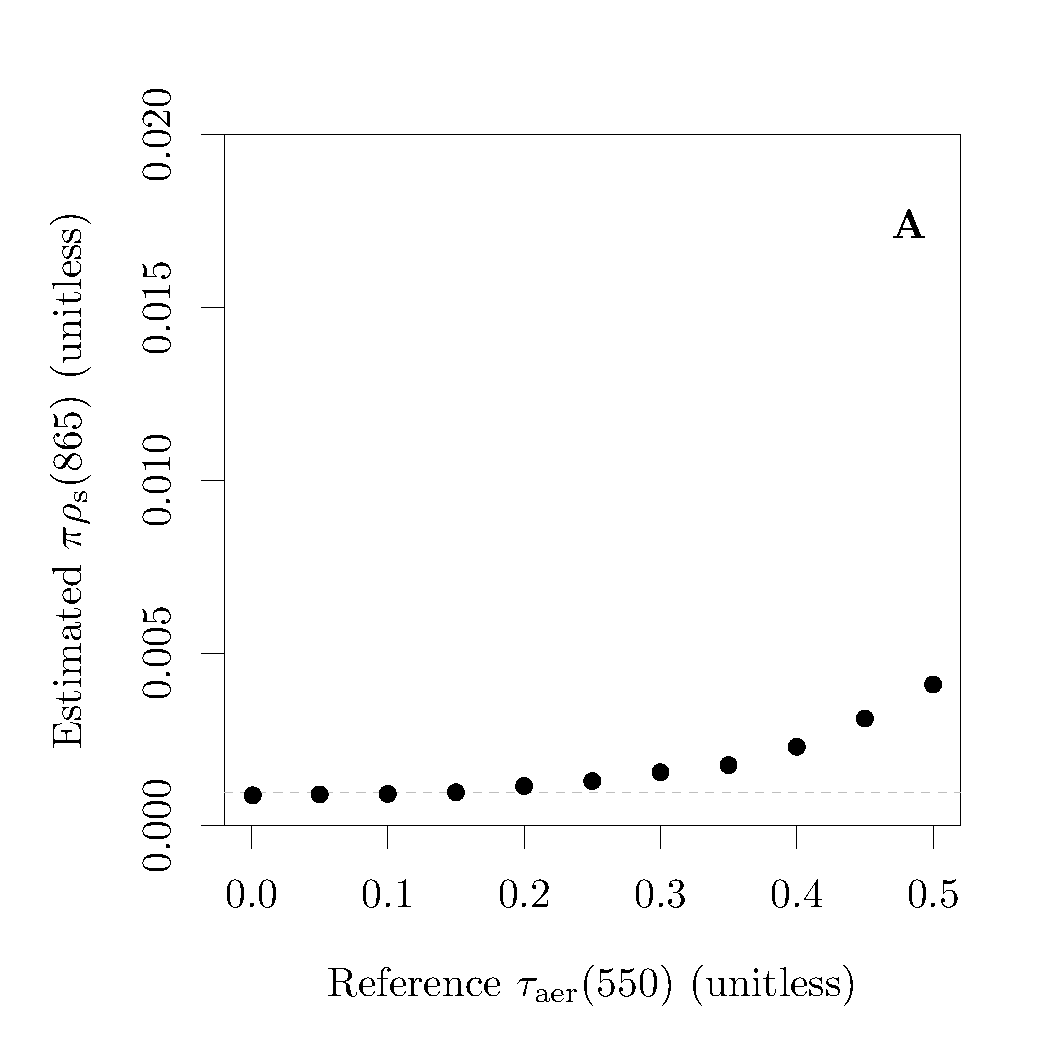
\includegraphics[trim={0 0.75cm 0 1cm},clip,width=\linewidth]{case_1_full_eval_c.pdf}
    \end{subfigure}
    \begin{subfigure}[t]{0.48\textwidth}
      \centering
      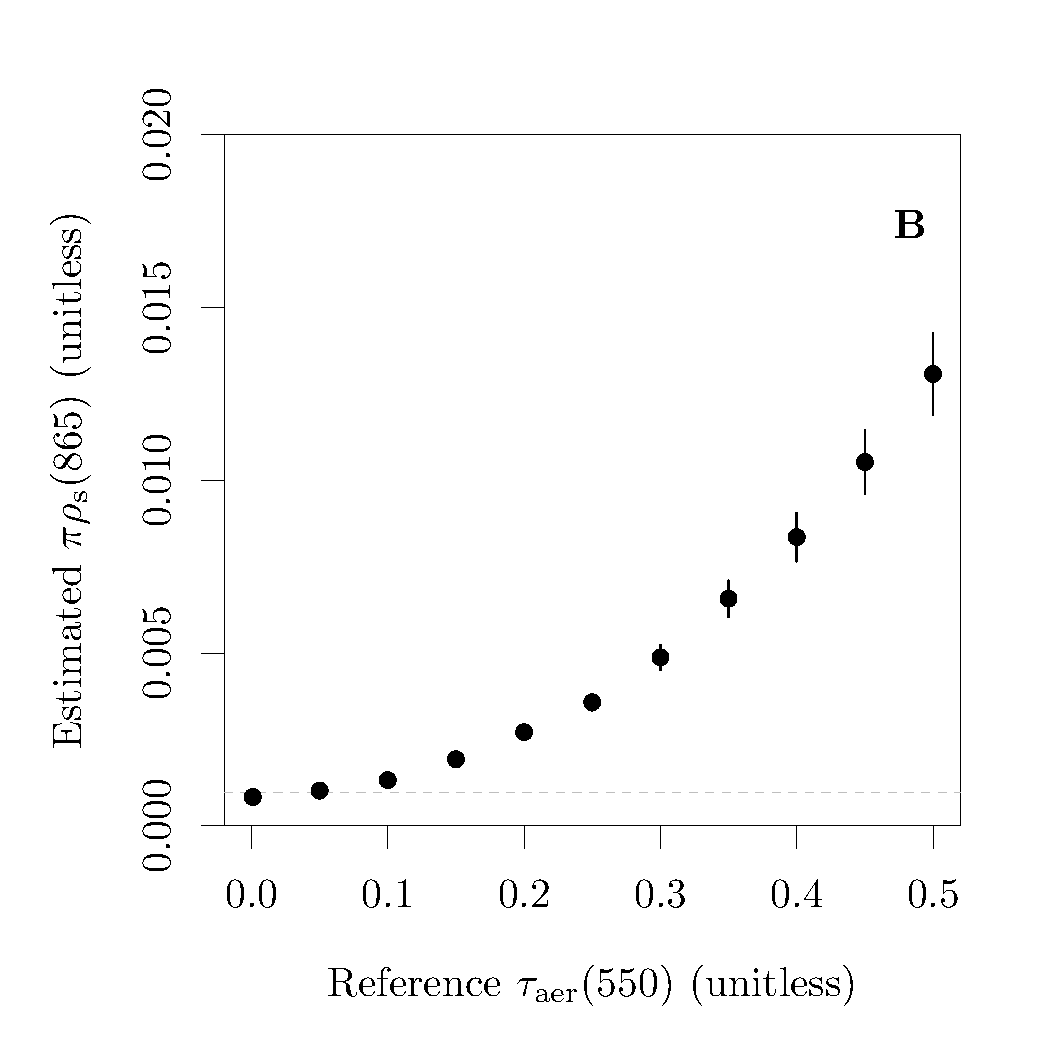
\includegraphics[trim={0 0.75cm 0 1cm},clip,width=\linewidth]{case_1_full_eval_m.pdf}
    \end{subfigure}
   \caption{Evaluation of $\smash{\rho_\text{s}}$ with the combination of TSDSF and RAdCor for the OLI waveband centred at 865~nm. (A) Estimation for the continental model simulation. (B) Estimation for the maritime model simulation. The grey horizontal line provides the reference $\smash{\pi\,\rho_\text{s}(865)}$ value.}
   \label{fig:sim01_full_eval}
\end{figure}





\chapter{Evaluation: Simulated scene 2} \label{ch:sim02}

This Chapter follows the same structure, analysis and visualisations as in Chapter~\ref{ch:sim01}, but for a simulation representing a coastal scene. Calculations are performed with Eq.~\ref{eq:theory_me_closed_form} to simulate the signal that would be observed over the Spuikom lagoon in Belgium, with the Operational Land Imager (OLI) onboard Landsat 8. The scene contains only two types of targets: water and vegetation (Fig.~\ref{fig:sim02_surf_setup}A). Water is represented by the Spuikom lagoon, channels and the Belgian coastal zone (Fig.~\ref{fig:sim02_surf_setup}B). The major axis of the Spuikom lagoon is $\approx$ 1.4 km long.

The atmospheric properties, calculated with 6SV, are the same as presented in Fig.~\ref{fig:sim01_atm_setup}. The resulting hemispherical-directional environmental reflectance for the upward diffuse transmittance, $\smash{\rho_{\text{s}_{\curlywedge_\text{b}^*}}(\hemidn \rightarrow \hat{\xi}_\text{D}; \Lambda_w; \vec{x})}$, and the bi-hemispherical environmental reflectance for the spherical albedo, $\smash{\rho_{\text{s}_{\curlyvee_\text{b}}}(\hemidn \rightarrow \hemiup; \Lambda_w; \vec{x})}$, for an $\smash{\tau_\text{aer}(865)}$ of 0.18~(unitless) are presented in Fig.~\ref{fig:sim02_env_averages}.

\begin{figure}[!htbp]
  \centering
    \begin{subfigure}[t]{0.48\textwidth}
      \centering
      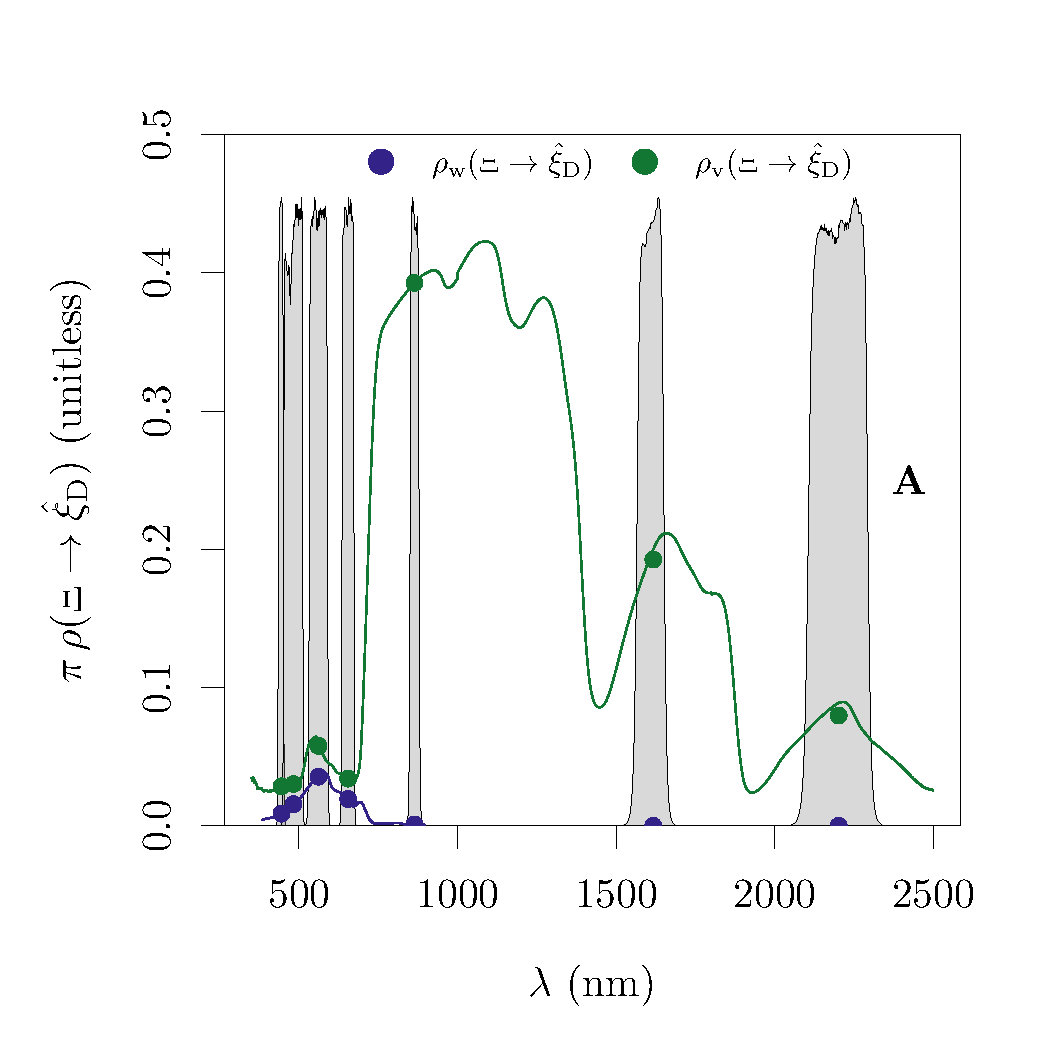
\includegraphics[trim={0 0.75cm 0 1cm},clip,width=\linewidth]{base_spectra.pdf}
    \end{subfigure}
    \begin{subfigure}[t]{0.48\textwidth}
      \centering
      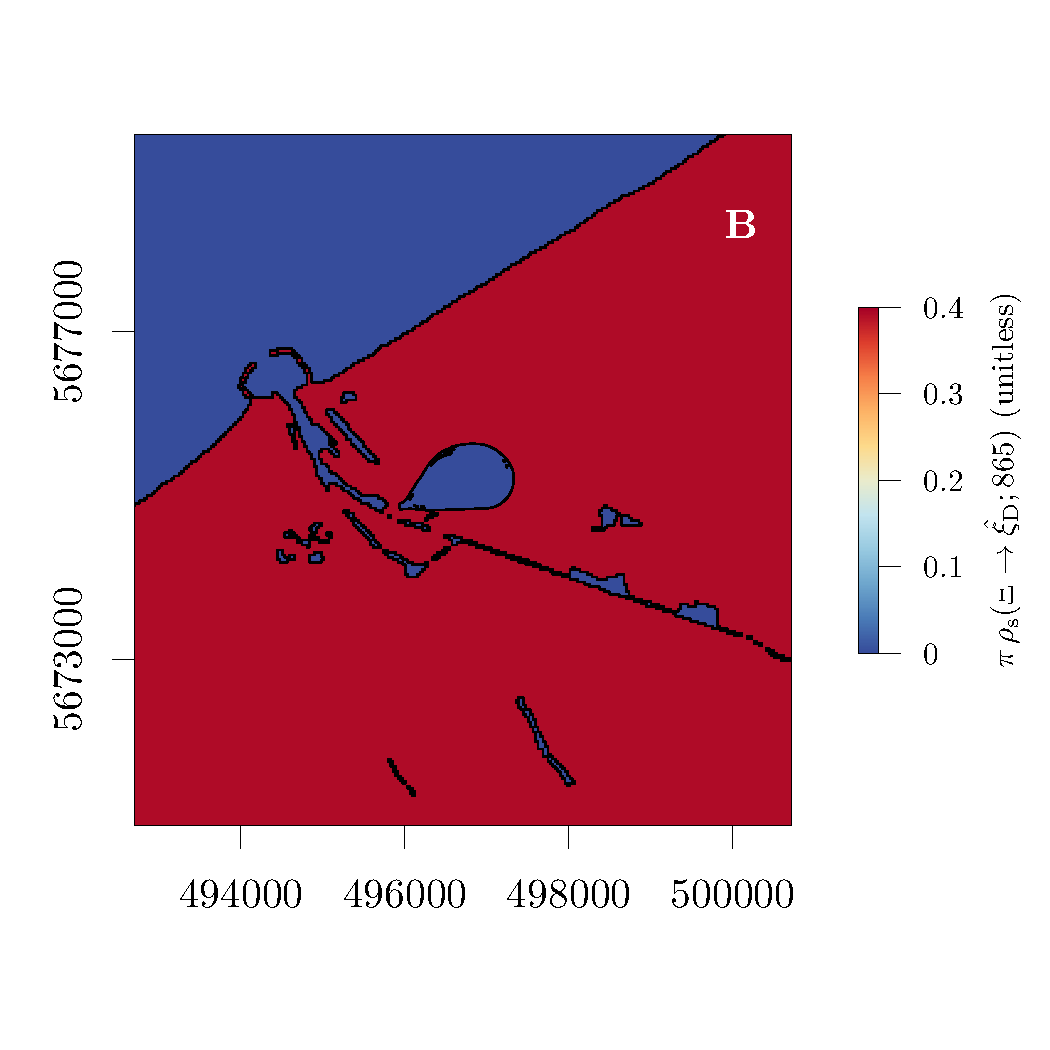
\includegraphics[trim={0 0.75cm 0 1cm},clip,width=\linewidth]{case_2_rho_s.pdf}
    \end{subfigure}
   \caption{Surface reflectance used in the simulation simulation. (A) Spectral hemispherical-directional reflectance of surface targets, scaled by $\smash{\pi}$~sr. (B) Surface pattern of the hemispherical-directional surface reflectance scaled by $\smash{\pi}$~sr for NIR waveband of OLI. In (A), subscript `w' stands for `water' and subscript `v' stands for `vegetation'. The grey polygons in the background show the relative spectral response functions of the first seven OLI wavebands.}
   \label{fig:sim02_surf_setup}
\end{figure}

\begin{figure}[!htbp]
  \centering
    \begin{subfigure}[t]{0.48\textwidth}
      \centering
      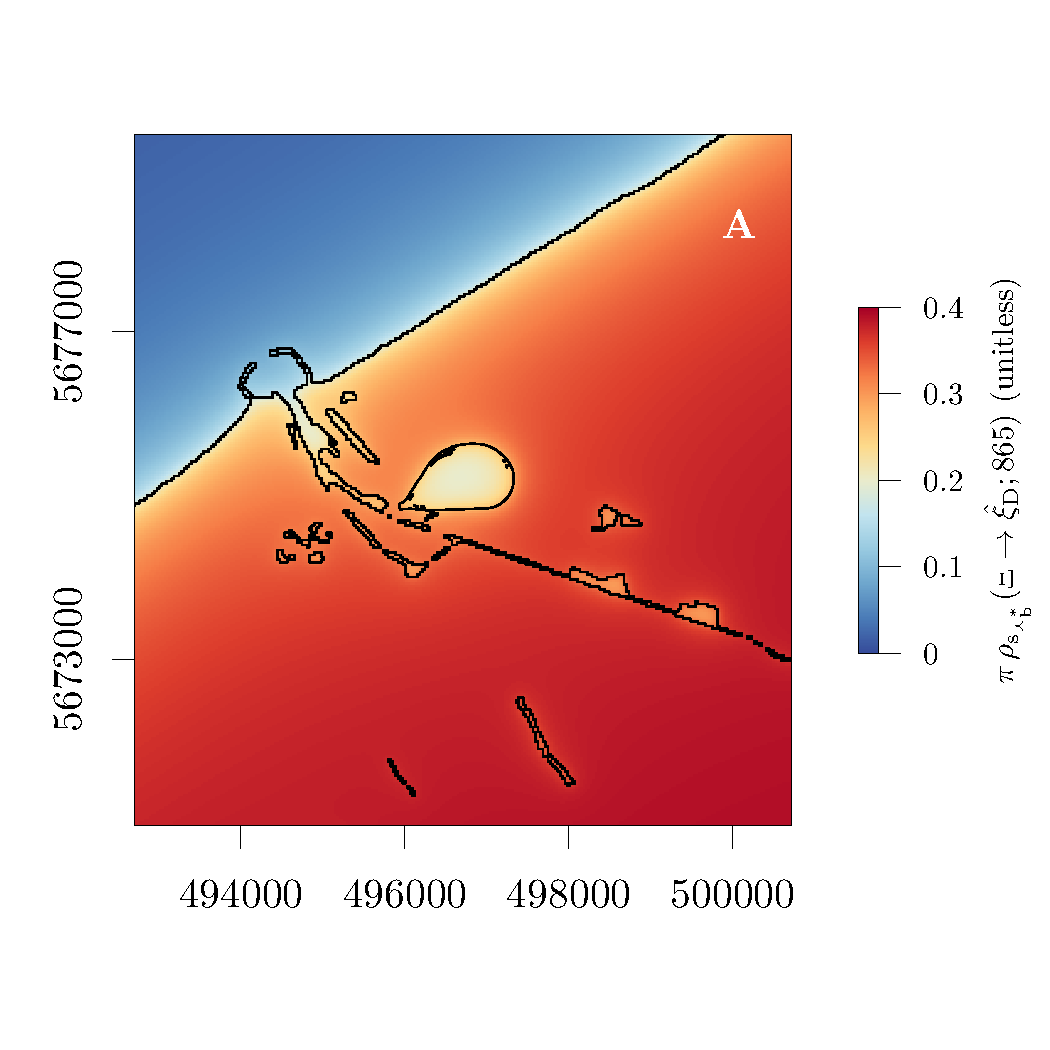
\includegraphics[trim={0 2cm 0 1cm},clip,width=\linewidth]{case_2_rho_env_psf_c.pdf}
    \end{subfigure}
    \begin{subfigure}[t]{0.48\textwidth}
      \centering
      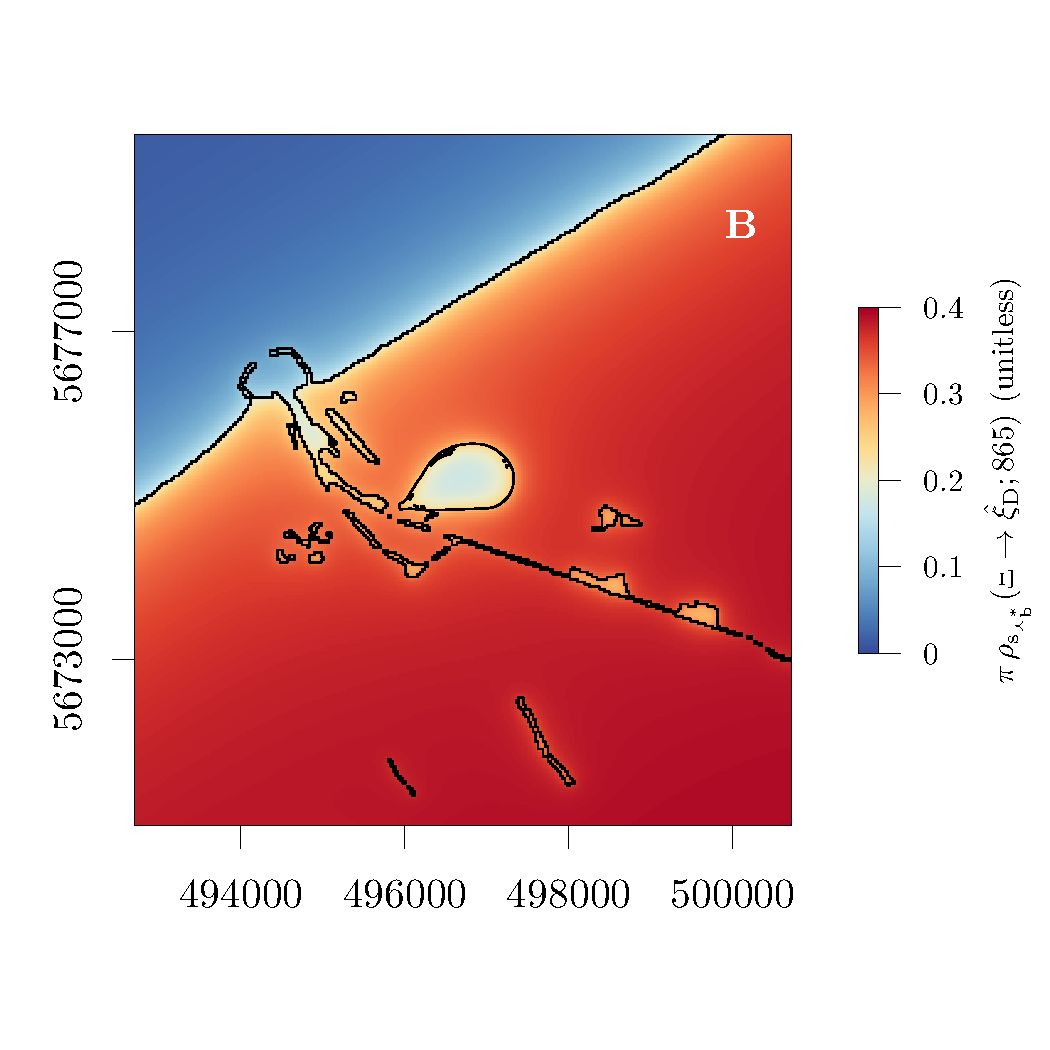
\includegraphics[trim={0 2cm 0 1cm},clip,width=\linewidth]{case_2_rho_env_psf_m.pdf}
    \end{subfigure}

    \begin{subfigure}[t]{0.48\textwidth}
      \centering
      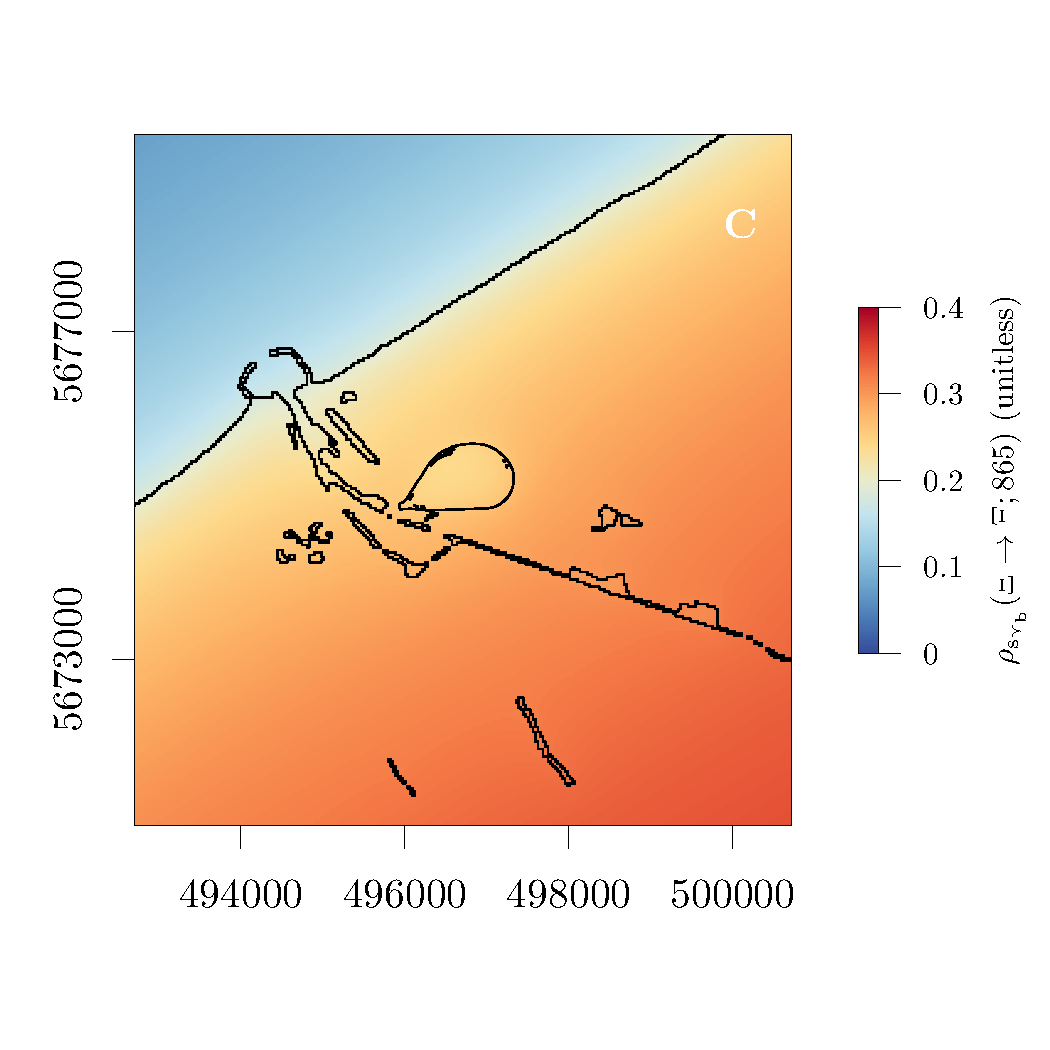
\includegraphics[trim={0 2cm 0 1cm},clip,width=\linewidth]{case_2_rho_env_sph_c.pdf}
    \end{subfigure}
    \begin{subfigure}[t]{0.48\textwidth}
      \centering
      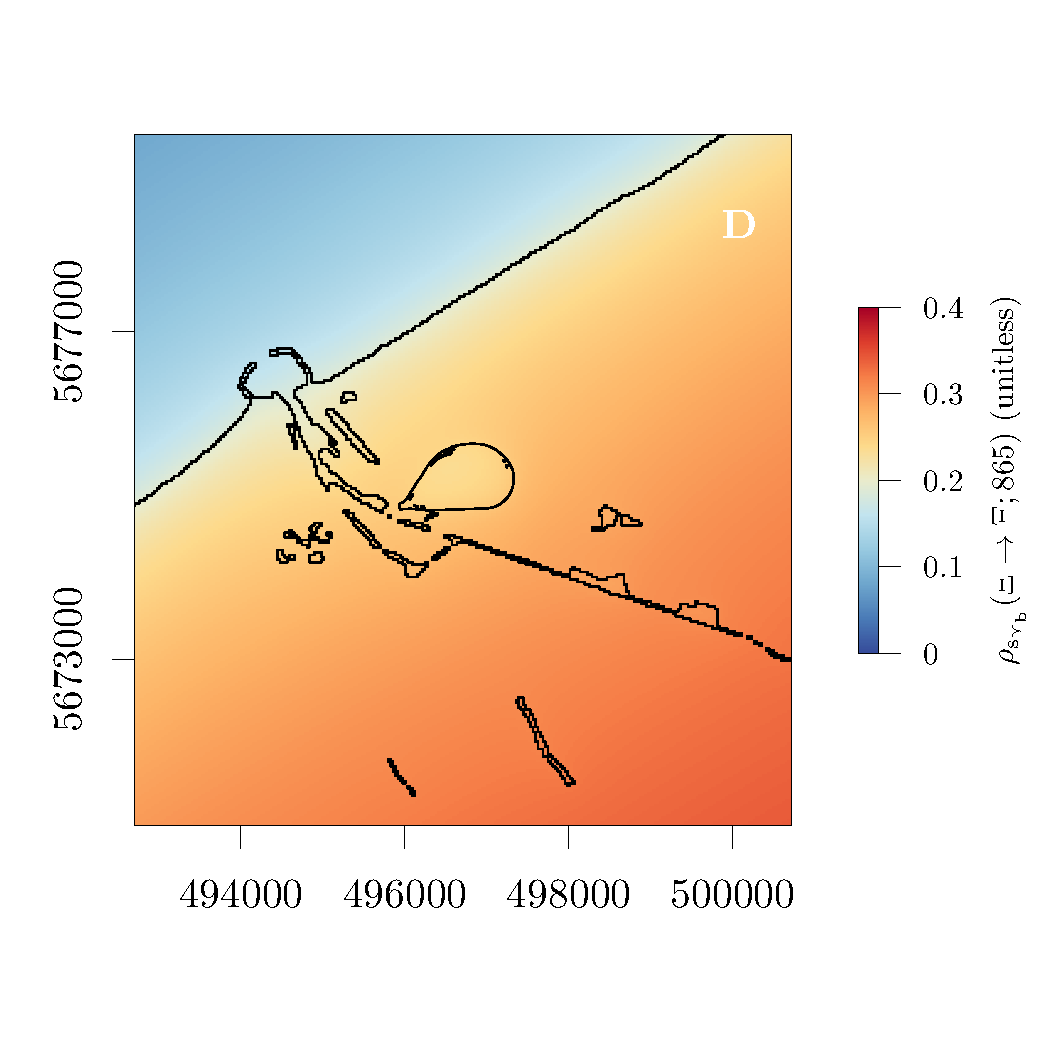
\includegraphics[trim={0 2cm 0 1cm},clip,width=\linewidth]{case_2_rho_env_sph_m.pdf}
    \end{subfigure}

   \caption{Environmental surface reflectances for an $\smash{\tau_\text{aer}(550)}$ of 0.3~(unitless). Hemispherical-directional environmental reflectance for the upward diffuse transmittance scaled by $\smash{\pi}$~sr, that is, the weighted average surface reflectance with weights given by $\smash{\hat{\curlywedge}_\text{b}(\hemiup \rightarrow \hat{\xi}_\text{D})}$, $\smash{\pi \, \rho_{\text{s}_{\curlywedge_\text{b}^*}}(\hemidn \rightarrow \hat{\xi}_\text{D})}$, for simulations with the continental aerosol model (A) and maritime aerosol model (B). Bi-hemispherical environmental reflectance for the spherical albedo, that is, the weighted average bi-hemispherical surface reflectance with weights given by $\smash{\hat{\curlyvee}_\text{b}(\hemiup \rightarrow \hemidn)}$, $\smash{\rho_{\text{s}_{\curlyvee_\text{b}}}(\hemidn \rightarrow \hemiup)}$, for simulations with the continental aerosol model (C) and maritime aerosol model (D). All variables presented for the NIR waveband of OLI, centred at wavelength 865~nm.}
   \label{fig:sim02_env_averages}
\end{figure}

\section{Evaluation of TSDSF}

As in Chapter~\ref{ch:sim01}, we let the predefined $\smash{\tau_\text{aer}(550)}$ be equal to the $\smash{\tau_\text{aer}(550)}$ used in the simulations and use a large PSF radius (25~km), to isolate the error of the approximation described in Eq.~\ref{eq:est_rho_e_toa} from other source of errors. Fig.~\ref{fig:sim02_hyp_estimate} shows the ratio of the estimated function, $\smash{\rho_\text{as}^\text{Hyp Est.}}$, to the reference function, $\smash{\rho_\text{as}^\text{Hyp Ref.}}$, calculated with Eq.~\ref{eq:ret_rho_env_toa} for an $\smash{\tau_\text{aer}(865)}$ of 0.18~(unitless). For those example conditions, the maximum error in the estimation was $< 15$~\% for simulations with both aerosol models. The higher values were observed at intermediate distances from the coast for the maritime aerosol model, and were higher than the maximum error of $< 10$~\% for the inland simulation.

\begin{figure}[!htbp]
  \centering
    \begin{subfigure}[t]{0.48\textwidth}
      \centering
      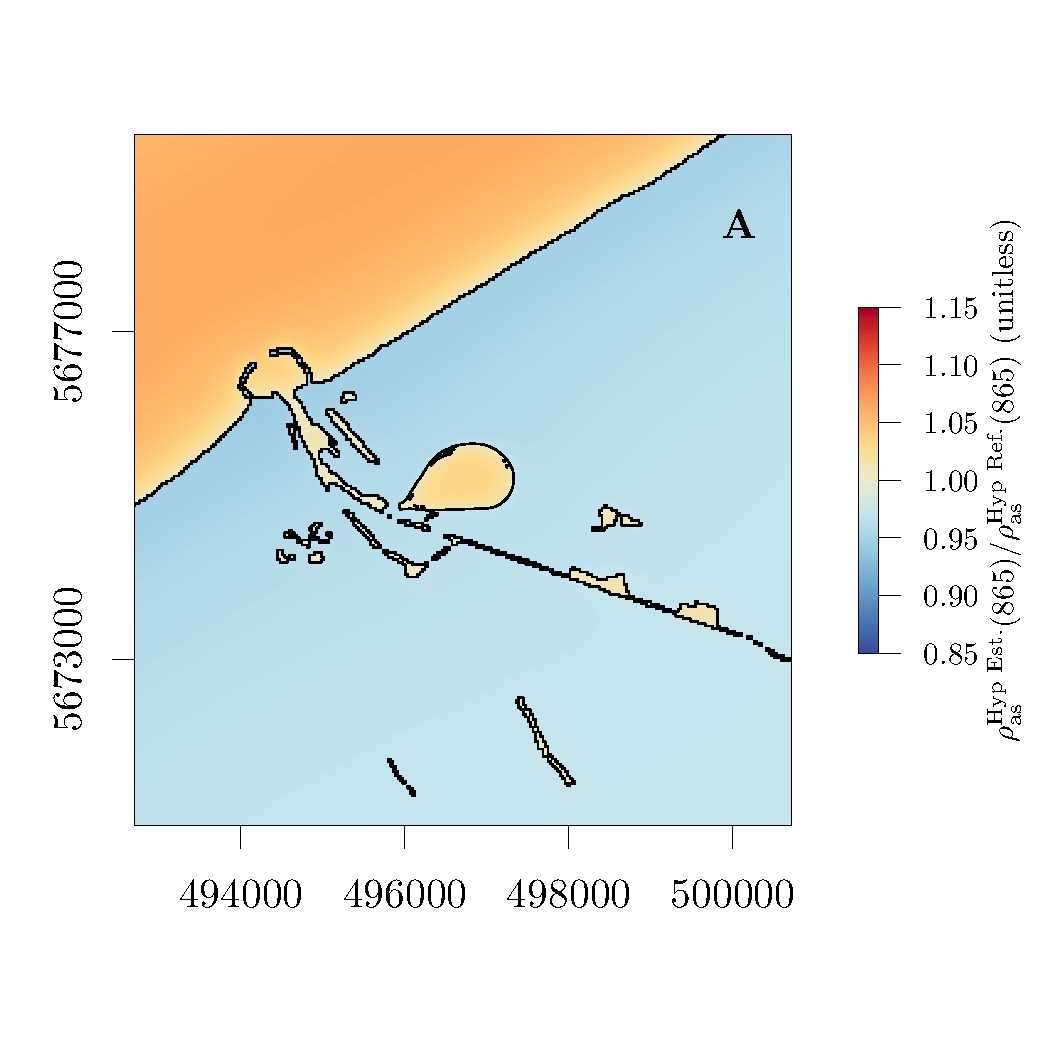
\includegraphics[trim={0 2cm 0 1cm},clip,width=\linewidth]{case_2_eval_rho_env_toa_c.pdf}
    \end{subfigure}
    \begin{subfigure}[t]{0.48\textwidth}
      \centering
      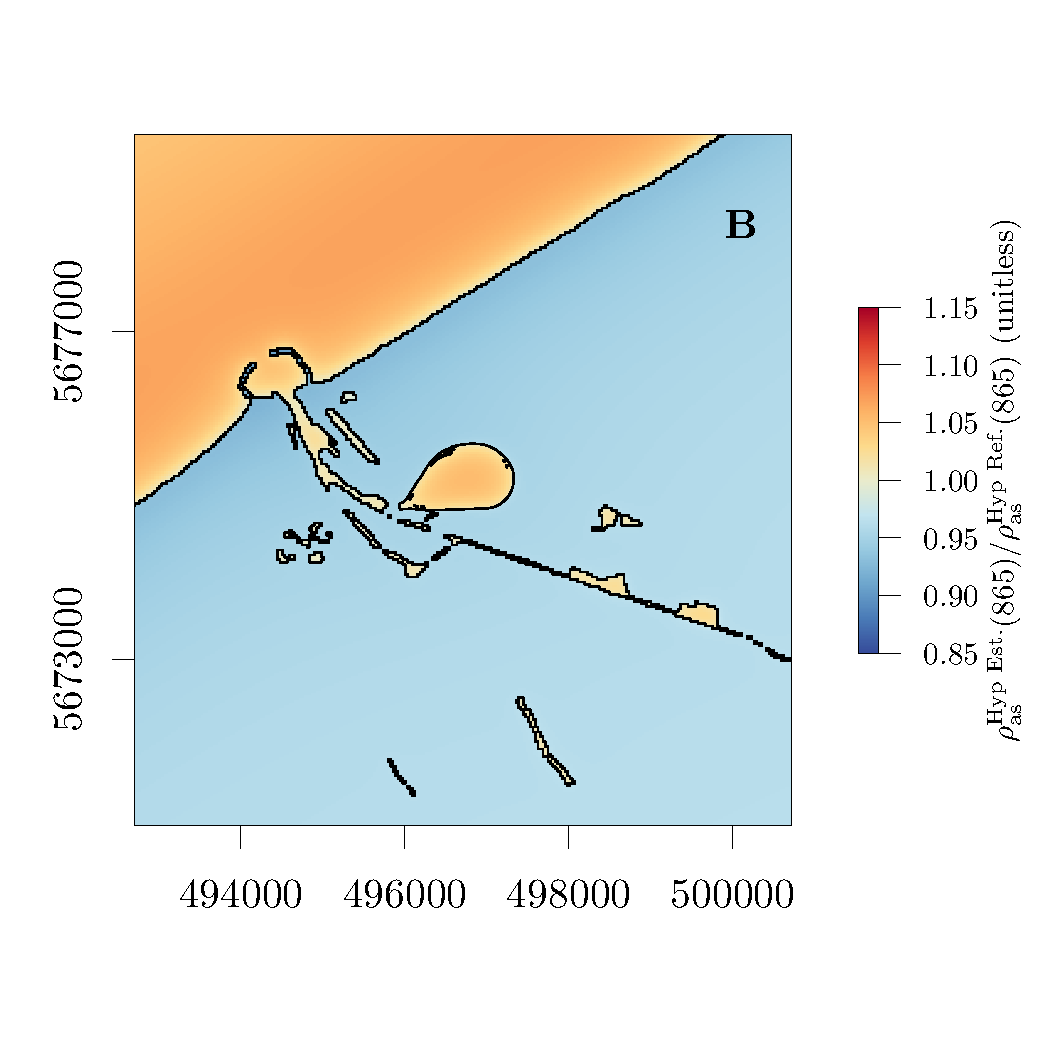
\includegraphics[trim={0 2cm 0 1cm},clip,width=\linewidth]{case_2_eval_rho_env_toa_m.pdf}
    \end{subfigure}
    
   \caption{Evaluation of the estimation of $\smash{\rho_\text{as}^\text{Hyp}(\hat{\xi}_0 \rightarrow \hat{\xi}_\text{D}; \Lambda_w; \vec{x})}$ from $\smash{\rho_\text{as}(\hat{\xi}_0 \rightarrow \hat{\xi}_\text{D}; \Lambda_w; \vec{x})}$. (A) Ratio of $\smash{\rho_\text{as}^\text{Hyp Est.}}$ to $\smash{\rho_\text{as}^\text{Hyp Ref.}}$ for the simulation with the continental aerosol model; (B) same as (A) but for the simulation with the maritime aerosol model. ``Est.'' stands for estimated value and ``Ref.'' stands for reference value.}
   \label{fig:sim02_hyp_estimate}
\end{figure}

We evaluate the propagated uncertainty through TSDSF using the $\tau_\text{aer}(550)$ estimation error as a metric. First we evaluate the impact of different predefined values of $\tau_\text{aer}(550)$, isolating it from errors related to the finite PSF by using a large PSF radius~(25 km). The results, presented in Fig.~\ref{fig:sim02_tsdsf_all_aot}, for a wide range of reference and predefined $\tau_\text{aer}(550)$ show the same main patterns as observed for the inland scene in Chapter~\ref{ch:sim01}: (1) There is an overall tendency of underestimation of $\tau_\text{aer}(550)$ which is proportional to the $\tau_\text{aer}(550)$ used in the simulation. (2) The estimation improves for all simulated $\tau_\text{aer}(550)$ for larger values of predefined $\tau_\text{aer}(550)$. Further, in specific circumstances, TSDSF estimates the incorrect aerosol model for maritime aerosol simulations, resulting also in larger errors in $\tau_\text{aer}(550)$ estimation. However, the magnitude of the reference $\tau_\text{aer}(550)$ at which the underestimation of $\tau_\text{aer}(550)$ became significant was larger than for the inland scene, likely due to the larger water surface in the coastal scene, indicating that the maximum atmospheric turbidity at which TSDSF is expected to provide a good estimation of aerosol properties will depend on the scene composition.

\begin{figure}[!htbp]
  \centering
    \begin{subfigure}[t]{0.48\textwidth}
      \centering
      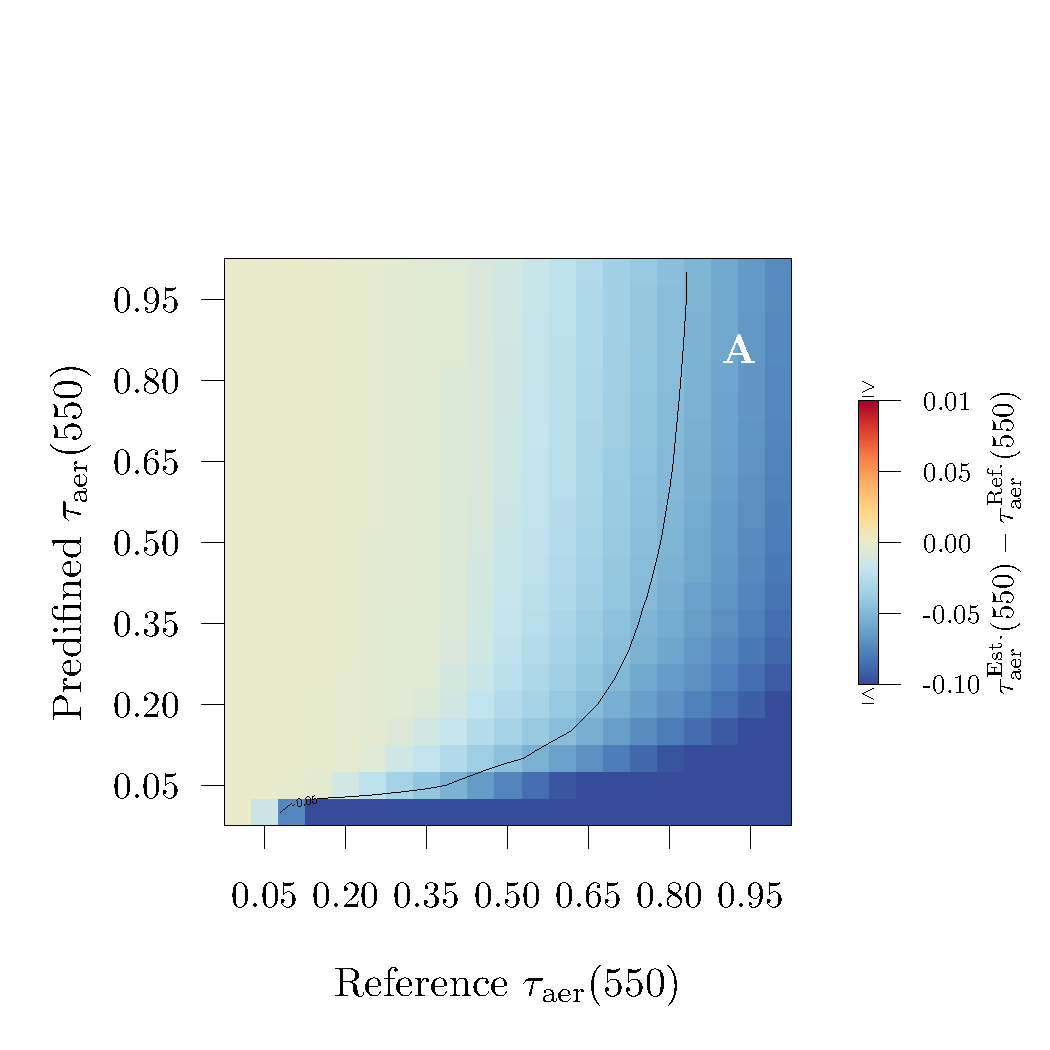
\includegraphics[trim={0 0.75cm 0 1cm},clip,width=\linewidth]{case_2_eval_ts_dsf_aot_c.pdf}
    \end{subfigure}
    \begin{subfigure}[t]{0.48\textwidth}
      \centering
      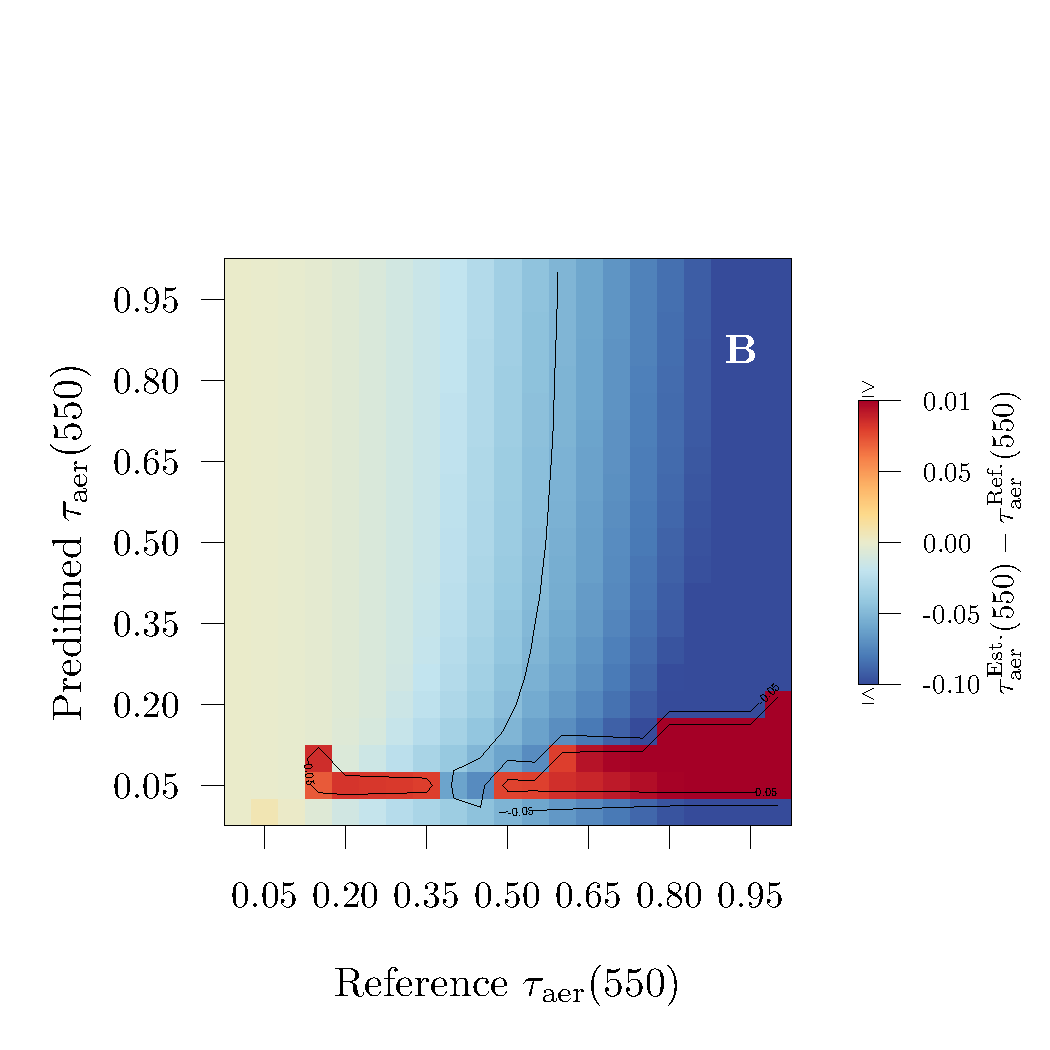
\includegraphics[trim={0 0.75cm 0 1cm},clip,width=\linewidth]{case_2_eval_ts_dsf_aot_m.pdf}
    \end{subfigure}
   \caption{TSDSF estimation error of $\tau_\text{aer}(550)$. $\tau_\text{aer}(550)$ estimation error for simulations with the continental aerosol model (A) and the maritime aerosol model (B). The X-axis provides the $\tau_\text{aer}(550)$ used in the simulation, while the Y-axis provides the $\tau_\text{aer}(550)$ used for the TSDSF estimation.}
   \label{fig:sim02_tsdsf_all_aot}
\end{figure}

The effect of the PSF extent on the TSDSF estimation was isolated by using the best predefined $\tau_\text{aer}(550)$ from the previous analysis, 1 (unitless), and evaluated by performing the TSDSF approach over a range of PSF radius from 2.5~km to 25~km. As for Fig.~\ref{fig:sim01_tsdsf_all_psf}, Fig.~\ref{fig:sim02_tsdsf_all_psf} shows that the $\tau_\text{aer}(550)$ estimation error is largely independent of PSF extent. 

\begin{figure}[!htbp]
  \centering
    \begin{subfigure}[t]{0.48\textwidth}
      \centering
      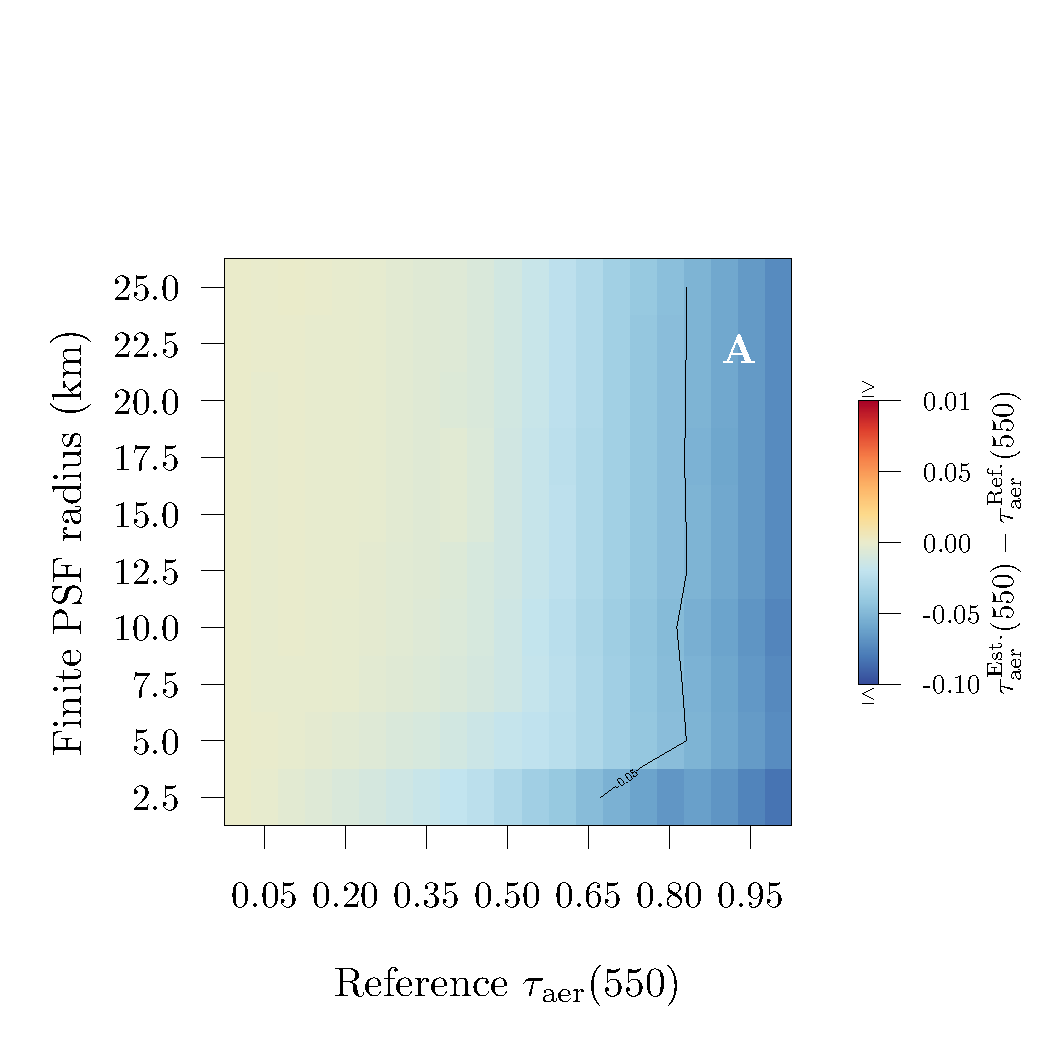
\includegraphics[trim={0 0.75cm 0 1cm},clip,width=\linewidth]{case_2_eval_ts_dsf_psf_c.pdf}
    \end{subfigure}
    \begin{subfigure}[t]{0.48\textwidth}
      \centering
      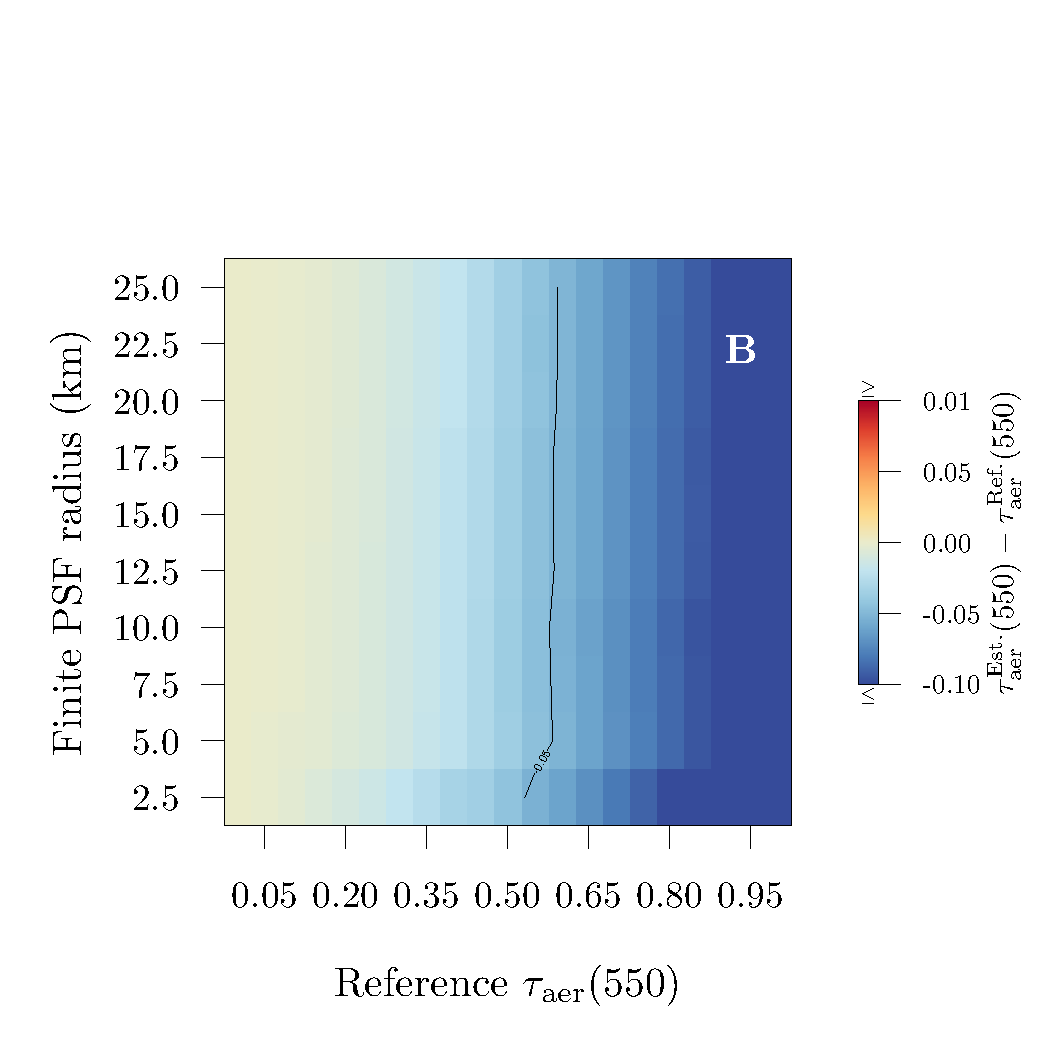
\includegraphics[trim={0 0.75cm 0 1cm},clip,width=\linewidth]{case_2_eval_ts_dsf_psf_m.pdf}
    \end{subfigure}
   \caption{TSDSF estimation error of $\tau_\text{aer}(550)$. $\tau_\text{aer}(550)$ estimation error for simulations with the continental aerosol model (A) and the maritime aerosol model (B). The X-axis provides the $\tau_\text{aer}(550)$ used in the simulation, while the Y-axis provides the PSF extent used for the TSDSF estimation.}
   \label{fig:sim02_tsdsf_all_psf}
\end{figure}

\section{Evaluation of RAdCor}

With the estimated aerosol model and concentration, the optical functions of the atmosphere can be calculated. These, together with the estimation of $\smash{\rho_{\text{s}_{\curlyvee_\text{b}}}(\hemidn \rightarrow \hemiup; \Lambda_w; \vec{x})}$, can be plugged in to Eq.~\ref{eq:radcor_lambertian_scene_fourier_finite} to retrieve $\smash{\rho_\text{s}(\hemidn \rightarrow \hat{\xi}_\text{D}; \Lambda_W; \vec{x})}$.

The approximations required to estimate $\smash{\rho_{\text{s}_{\curlyvee_\text{b}}}(\hemidn \rightarrow \hemiup; \Lambda_w; \vec{x})}$ are evaluated directly by setting the aerosol model and $\tau_\text{aer}(550)$ to the same values used in the simulation, and by using a PSF extent of 25~km. Fig.~\ref{fig:sim02_env_sph_est} shows an example for the simulations with $\tau_\text{aer}(550) = 0.3$ (unitless). Errors were $< 10$~\%, higher than the errors for the coastal scene ($< 5$~\%). Interestingly, the intense blurring resulted in an error gradient following the orientation of the coastline. This can be expected due to the large adjacent surfaces of water and land. This gradient was more intense for the maritime aerosol, again related to the larger forward peak of its scattering phase function when compared to the continental aerosol model. Though the errors in the estimation of $\smash{\rho_{\text{s}_{\curlyvee_\text{b}}}(\hemidn \rightarrow \hemiup; \Lambda_w; \vec{x})}$ were higher and the spatial contrast of $\smash{\rho_{\text{s}_{\curlyvee_\text{b}}}(\hemidn \rightarrow \hemiup; \Lambda_w; \vec{x})}$ (Fig.~\ref{fig:sim02_env_averages}C and D) was also higher than for the inland simulation, the evaluation of the retrieved surface reflectances suggests that the approximation given by Eq.~\ref{eq:radcor_rho_env_sph} is still valid.

\begin{figure}[!htbp]
  \centering
    \begin{subfigure}[t]{0.48\textwidth}
      \centering
      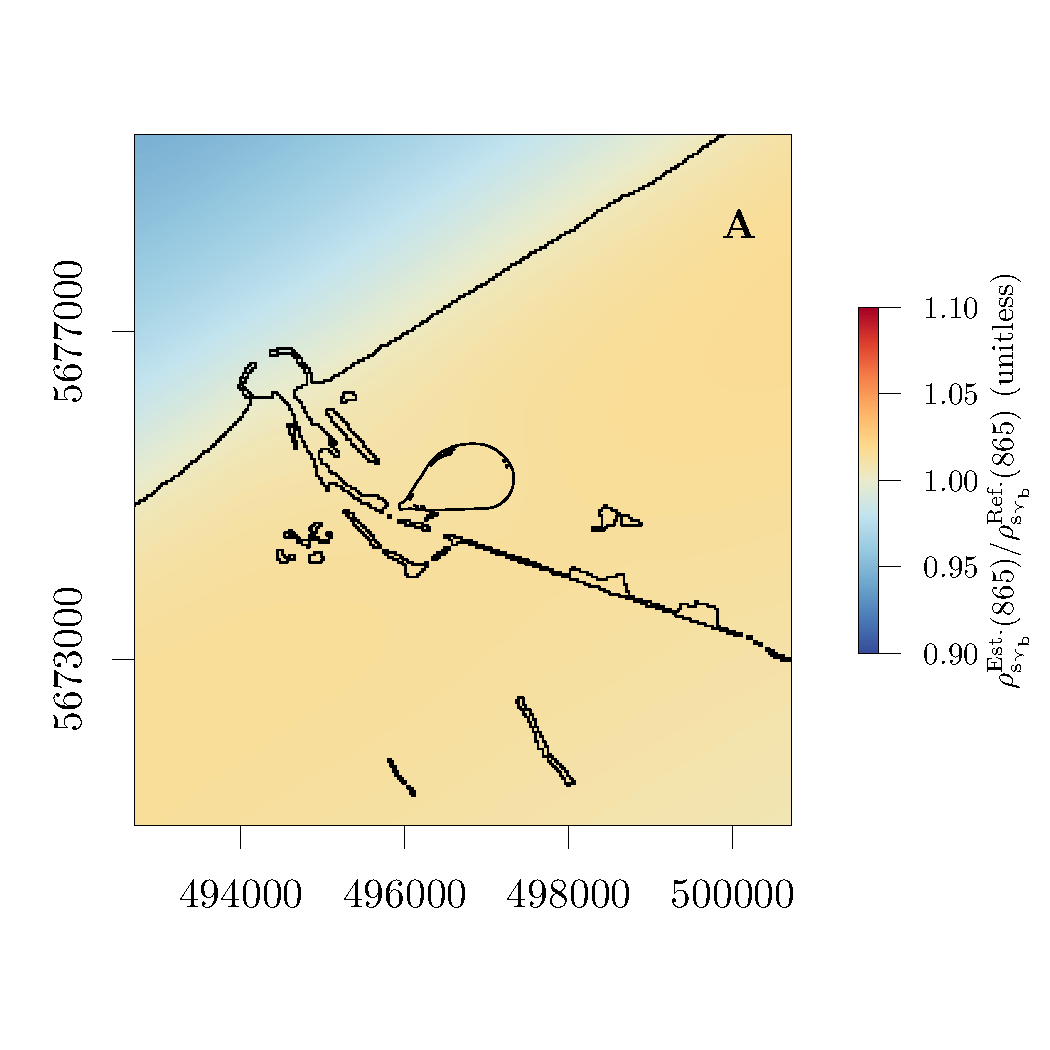
\includegraphics[trim={0 2cm 0 1cm},clip,width=\linewidth]{case_2_eval_rho_env_sph_c_est.pdf}
    \end{subfigure}
    \begin{subfigure}[t]{0.48\textwidth}
      \centering
      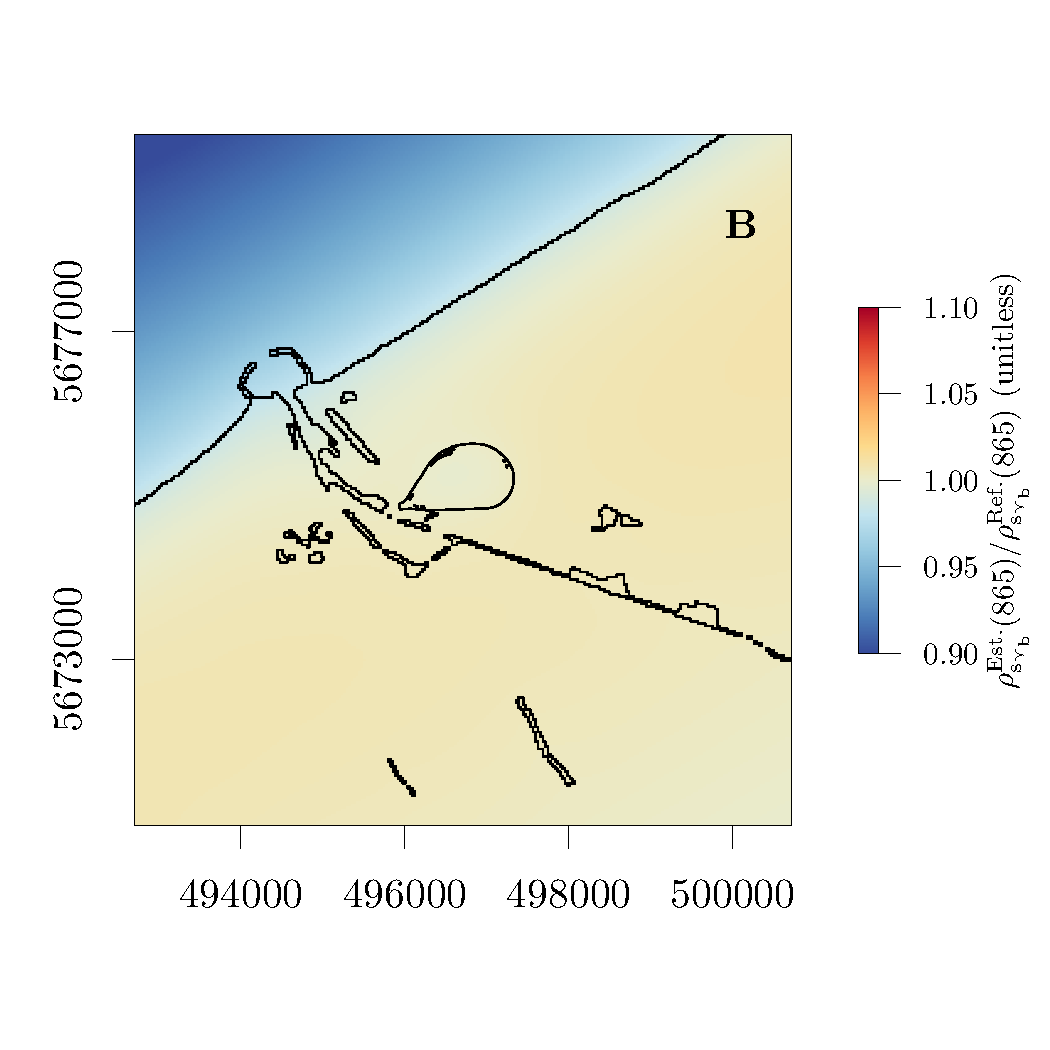
\includegraphics[trim={0 2cm 0 1cm},clip,width=\linewidth]{case_2_eval_rho_env_sph_m_est.pdf}
    \end{subfigure}
   \caption{Evaluation of the $\smash{\rho_{\text{s}_{\curlyvee_\text{b}}}(\hemidn \rightarrow \hemiup; \Lambda_w; \vec{x})}$ estimate against the reference value calculated with Eq.~\ref{eq:theory_bhem} for the OLI waveband centered at 865~nm. (A) Ratio for the Continental model simulation; (B) Ratio for the Maritime model simulation.}
   \label{fig:sim02_env_sph_est}
\end{figure}

We again isolate the effect of the PSF extent by performing the atmospheric correction using the reference $\tau_\text{aer}(550)$ and aerosol model, an evaluate the retrieval over a range of PSF radius. Fig.~\ref{fig:sim01_radcor_all} shows the average surface reflectance estimation error over the Spuikom lagoon. Here, the improvement in the retrievals with larger PSF radius, with the lower boundary dependent on the $\tau_\text{aer}(550)$ used in the simulation, seen for the inland simulation was not observed. The minimum PSF radius was approximately constant around 10~km regardless of the reference $\tau_\text{aer}(550)$ used in the simulations. As noted in Chapter~\ref{ch:sim01}, preliminary evaluations with real imagery showed little improvement for kernel radius above 5~km.

\begin{figure}[!htbp]
  \centering
    \begin{subfigure}[t]{0.48\textwidth}
      \centering
      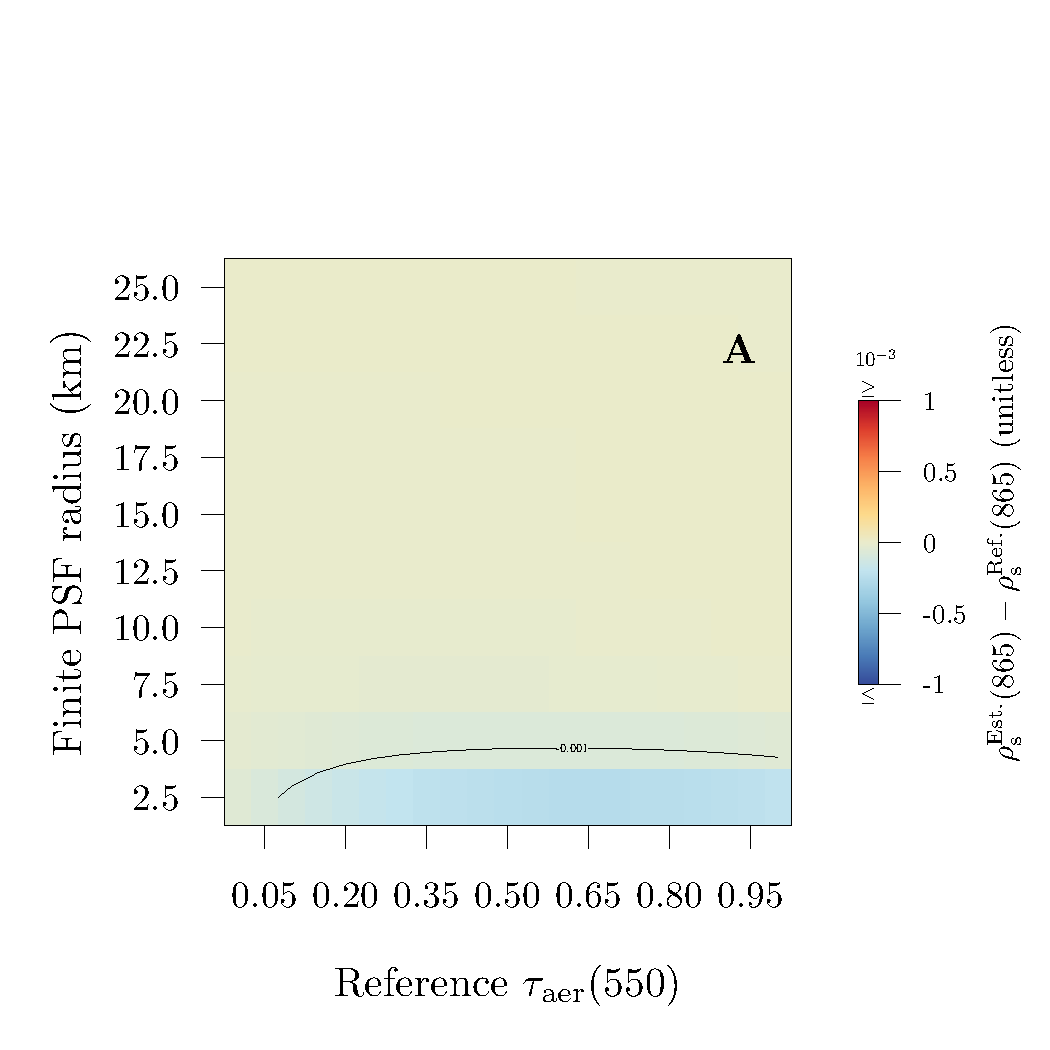
\includegraphics[trim={0 0.75cm 0 2.2cm},clip,width=\linewidth]{case_2_eval_radcor_abs_c}
    \end{subfigure}
    \begin{subfigure}[t]{0.48\textwidth}
      \centering
      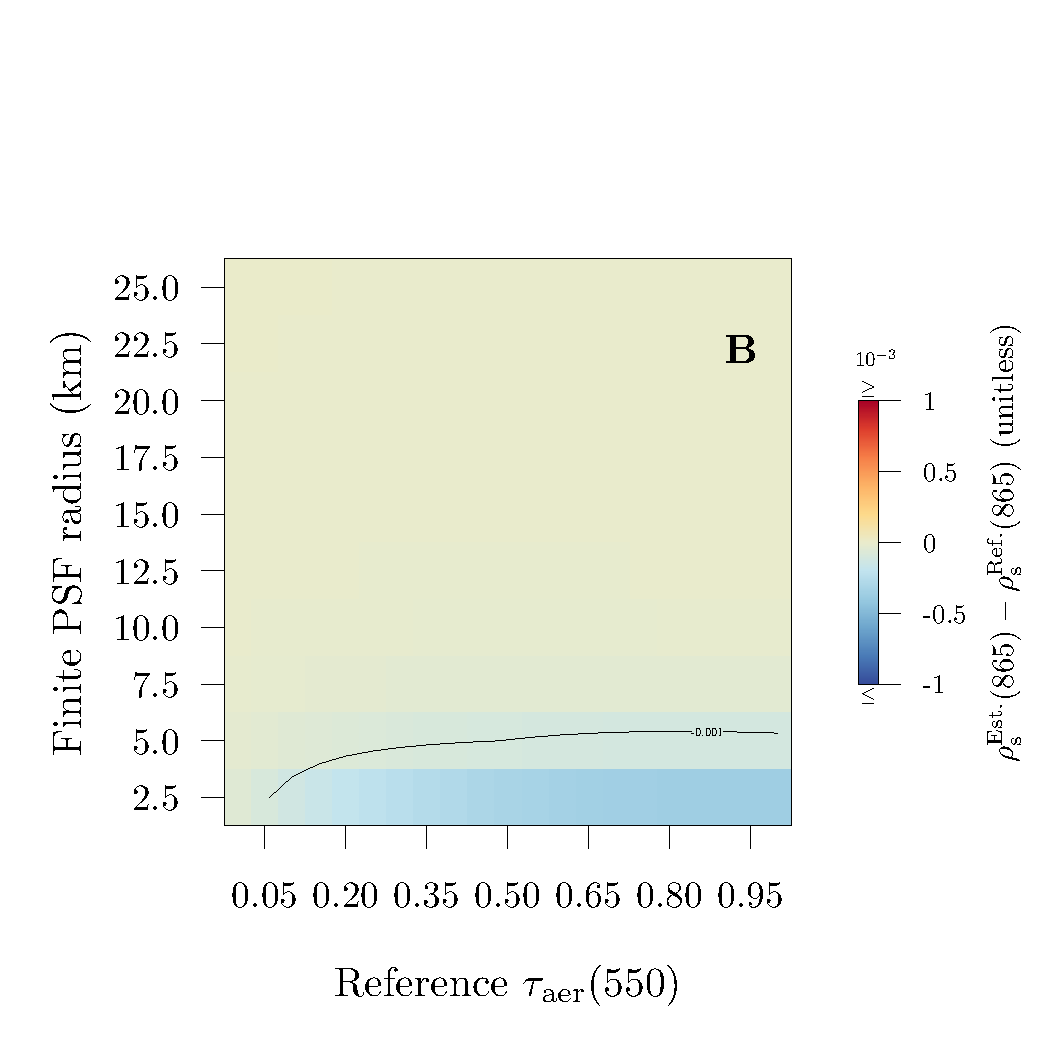
\includegraphics[trim={0 0.75cm 0 2.2cm},clip,width=\linewidth]{case_2_eval_radcor_abs_m}
    \end{subfigure}
    
    \begin{subfigure}[t]{0.48\textwidth}
      \centering
      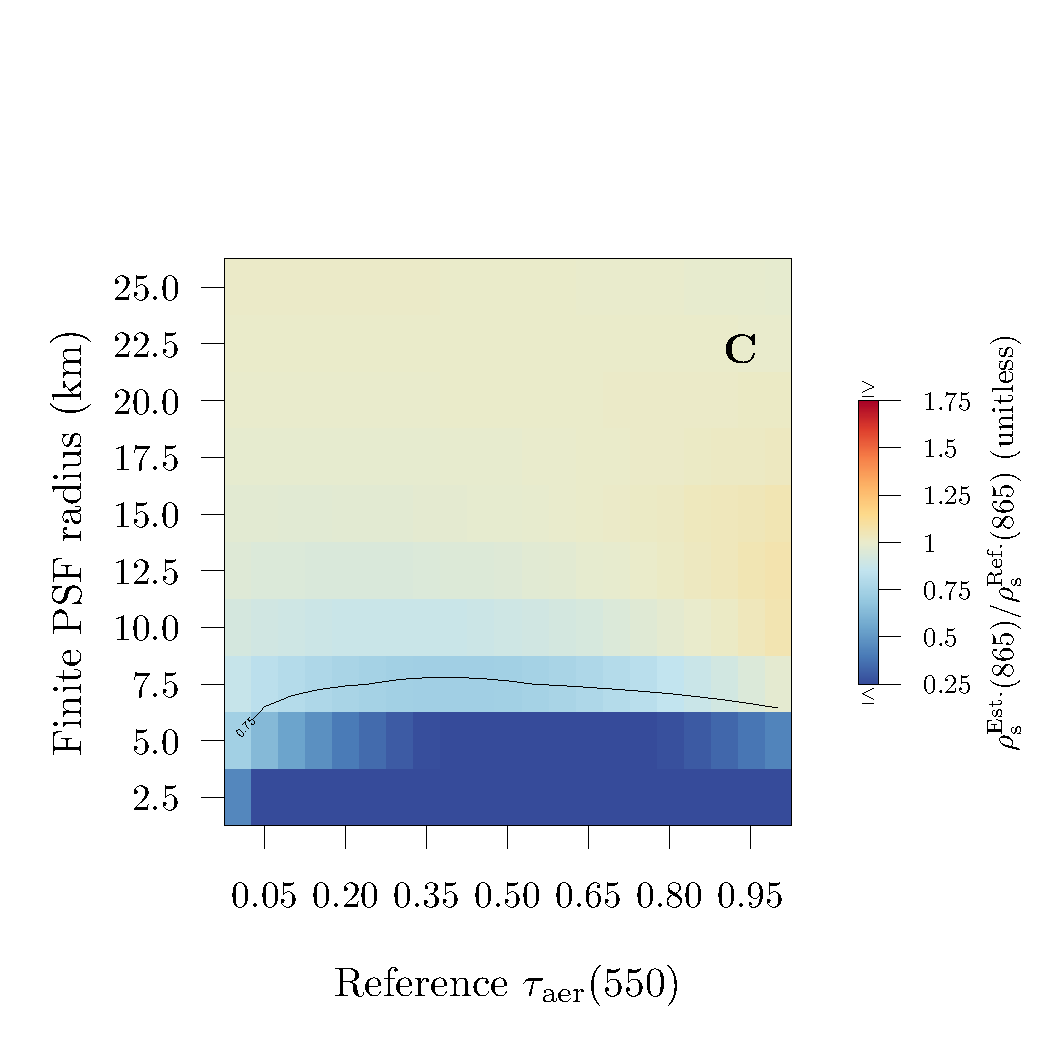
\includegraphics[trim={0 0.75cm 0 2.2cm},clip,width=\linewidth]{case_2_eval_radcor_rel_c}
    \end{subfigure}
    \begin{subfigure}[t]{0.48\textwidth}
      \centering
      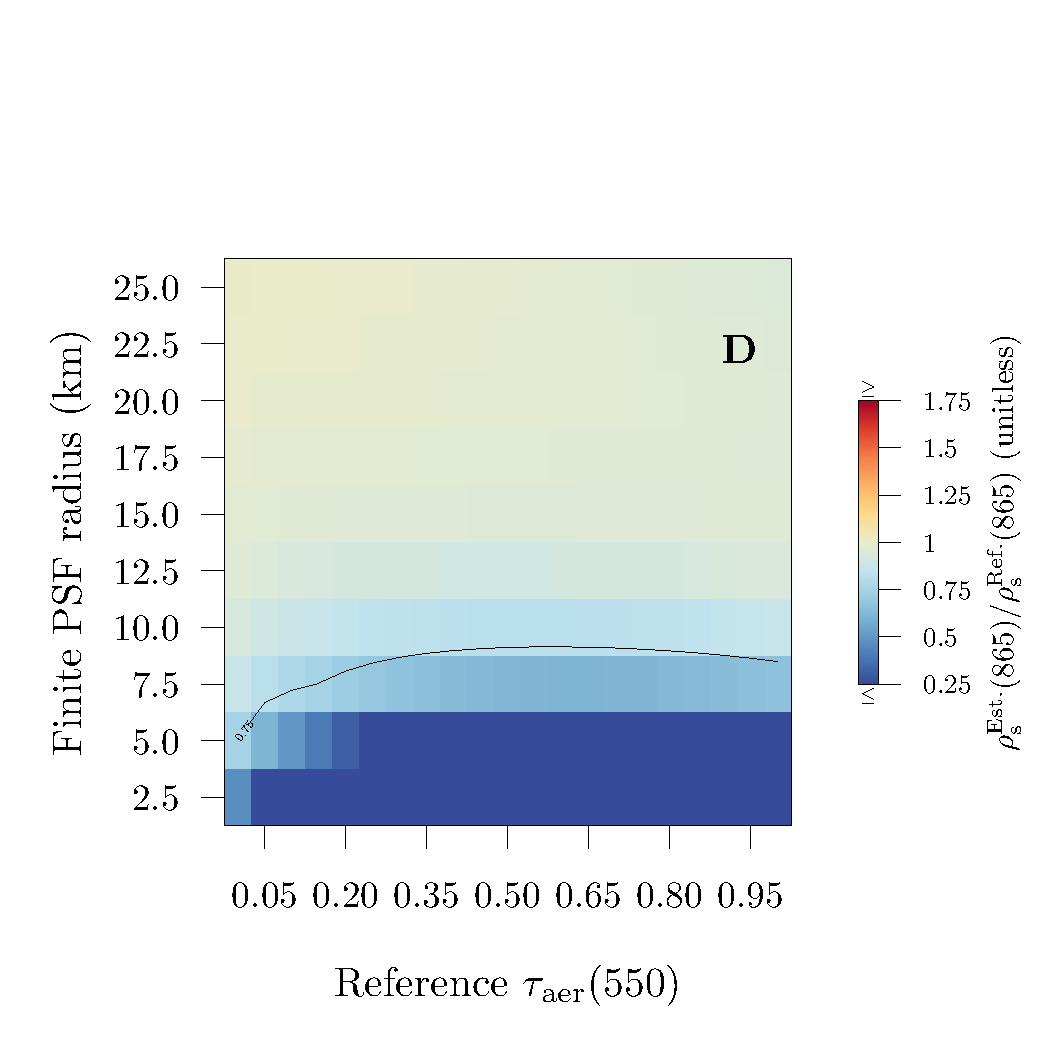
\includegraphics[trim={0 0.75cm 0 2.2cm},clip,width=\linewidth]{case_2_eval_radcor_rel_m}
    \end{subfigure}

   \caption{Evaluation of atmospheric correction over the Spuikom lagoon for different finite PSF radius. Difference between the average estimated surface reflectance and the reference reflectance for the continental model simulations (A) and maritime model simulations (B). Ratio of the average estimated surface reflectance and the reference reflectance for the continental model simulations (C) and maritime model simulations (D). The reference $\tau_\text{aer}(550)$ for each simulation was used for the correction.}
   \label{fig:sim02_radcor_all}
\end{figure}

\section{Combined evaluation of TSDSF and RAdCor}

Here, the aerosol properties used for the correction are taken from the TSDSF estimation. The impact of the underestimation of $\tau_\text{aer}(550)$ can be clearly seen in Fig.~\ref{fig:sim02_full_eval}. The larger errors for the maritime model in part result from its spectral properties (\textit{cf.} Fig.~\ref{fig:sph_albd_sim_saf}). The spectral properties of the maritime aerosol model result in higher $\tau_\text{aer}$ in the NIR and SWIR for a given $\tau_\text{aer}(550)$ when compared to the continental aerosol model. In the simulations, the lowest $\tau_\text{aer}(550)$ estimated with TSDSF per band was always from the NIR and SWIR bands. For the continental aeorsol model, these wavebands will present a lower atmospheric turbidity than for the maritime aerosol model at comparable $\tau_\text{aer}(550)$.

Despite the insights provided by the simulations, validation with real imagery will be necessary to evaluate which aspects of the interpretations from the analysis with simulated scenes are directly applicable to real imagery, specially the magnitudes of estimation errors. The validation with real imagery against in situ reference surface reflectance will be provided in a separate document.   

\begin{figure}[!htbp]
  \centering
    \begin{subfigure}[t]{0.48\textwidth}
      \centering
      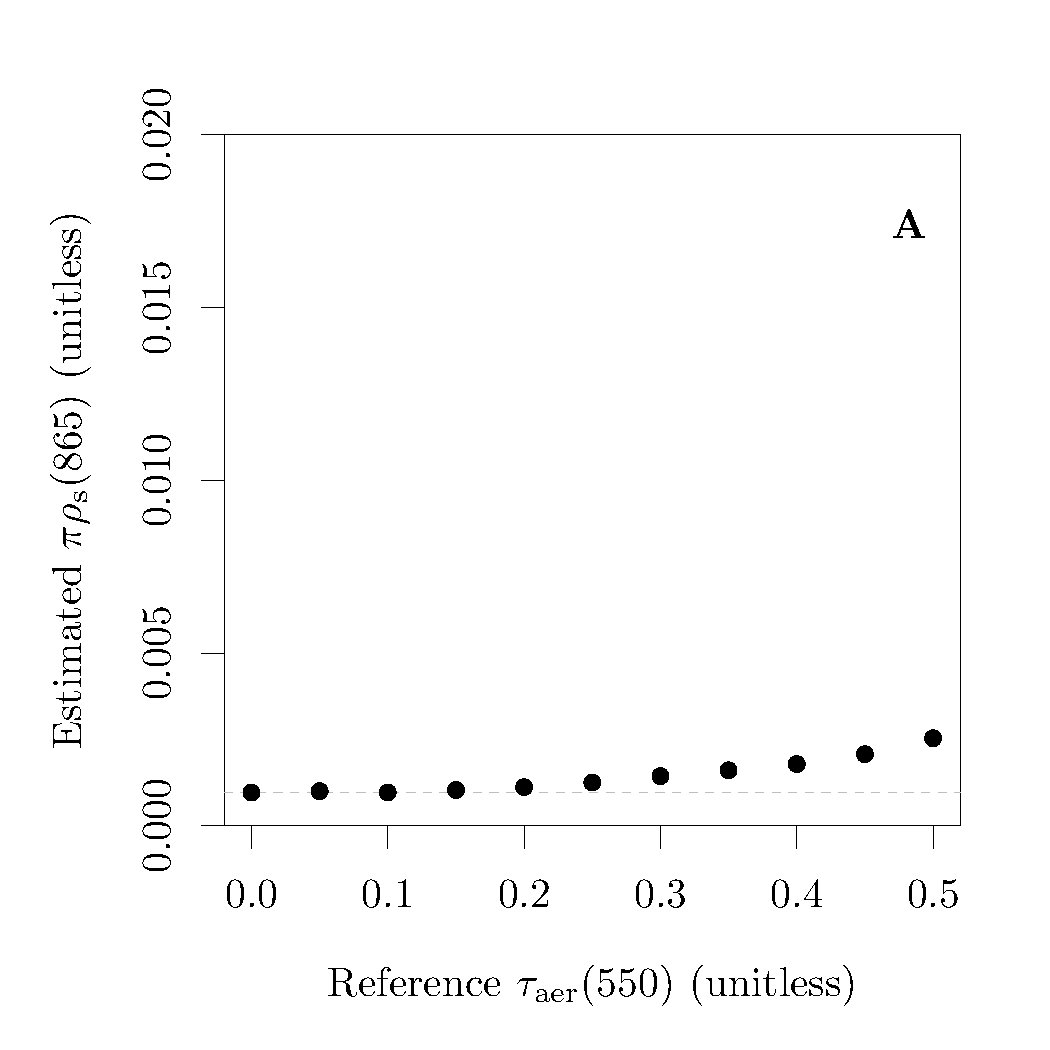
\includegraphics[trim={0 0.75cm 0 1cm},clip,width=\linewidth]{case_2_full_eval_c.pdf}
    \end{subfigure}
    \begin{subfigure}[t]{0.48\textwidth}
      \centering
      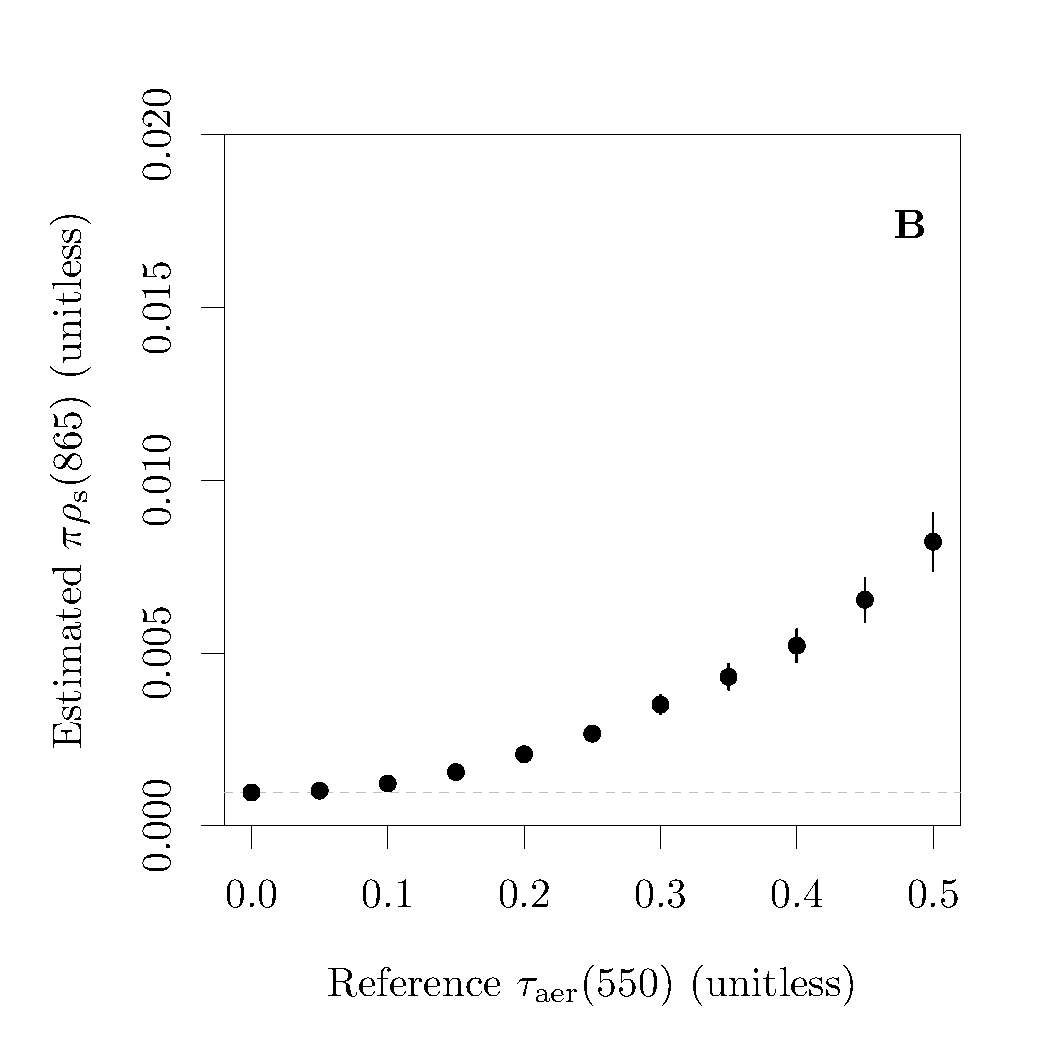
\includegraphics[trim={0 0.75cm 0 1cm},clip,width=\linewidth]{case_2_full_eval_m.pdf}
    \end{subfigure}
   \caption{Evaluation of $\smash{\rho_\text{s}}$ with the combination of TSDSF and RAdCor for the OLI waveband centred at 865~nm. (A) Estimation for the continental model simulation. (B) Estimation for the maritime model simulation. The grey horizontal line provides the reference $\smash{\pi\,\rho_\text{s}(865)}$ value.}
   \label{fig:sim02_full_eval}
\end{figure}


% ------------------------------------------------------------------------------
% Appendices 
% 

\begin{appendices}

\renewcommand{\thefigure}{\thechapter.\twodigits{\arabic{figure}}}
\renewcommand{\thetable}{\thechapter.\twodigits{\arabic{table}}}
\renewcommand{\theequation}{\thechapter.\twodigits{\arabic{equation}}}

\chapter{Pseudo-code: TSDSF} \label{ap:ts_dsf}

The pseudo-code of the TSDSF method to estimate aerosol model and optical thickness from TOA imagery is provided below:

\begin{enumerate}
    \item Retrieve the atmospheric pressure at the surface and the optical thickness of absorbing gases per waveband.
    \item Compensate $\smash{\rho_\text{as}(\hat{\xi}_0 \rightarrow \hat{\xi}_\text{D}; \Lambda_W; \vec{x})}$ for the transmittance of absorbing gases.
    \item If the finite integro-normalised diffuse PSF $\smash{\bunderline[4]{\hat{\curlywedge}}_\text{b}^*(\hemiup \rightarrow \hat{\xi}_\text{D}; \Lambda_w; \vec{x})}$ will not be re-normalised to integrate to unity, calculate the neighbourhood average $\smash{\overbar{\rho}_{\text{as}_\text{nb}}(\hat{\xi}_0 \rightarrow \hat{\xi}_\text{D}; \Lambda_w; \vec{x})}$ or the scene average $\smash{\overbar{\rho}_\text{as}(\hat{\xi}_0 \rightarrow \hat{\xi}_\text{D}; \Lambda_w)}$ to account for the missing upward diffuse transmittance due to the finite PSF, $\smash{1 - f_{\curlywedge_\text{b}^*}(\Lambda_w)}$.
    \item For each aerosol model:
        \begin{enumerate}
            \item Calculate $\smash{\bunderline[4]{\hat{\curlywedge}}_\text{b}^*(\hemiup \rightarrow \hat{\xi}_\text{D}; \Lambda_w; \vec{x})}$ for the preset value of $\smash{\tau_\text{aer}(550)} = 1$.
            \item Estimate $\smash{\rho_\text{as}^\text{Hyp}(\hat{\xi}_0 \rightarrow \hat{\xi}_\text{D}; \Lambda_w; \vec{x})}$ as the convolution of $\smash{\rho_\text{as}(\hat{\xi}_0 \rightarrow \hat{\xi}_\text{D}; \Lambda_w; \vec{x})}$ and $\smash{\bunderline[4]{\hat{\curlywedge}}_\text{b}^*(\hemiup \rightarrow \hat{\xi}_\text{D}; \Lambda_w; \vec{x})}$, accounting for the missing fraction $\smash{1 - f_{\curlywedge_\text{b}^*}(\Lambda_w)}$ if $\smash{\bunderline[4]{\hat{\curlywedge}}_\text{b}^*(\hemiup \rightarrow \hat{\xi}_\text{D}; \Lambda_w; \vec{x})}$ was not re-normalised.
            \item Identify the darkest pixels at the surface from pixels in the centre area of the scene with the lowest values of $\smash{\rho_\text{as}(\hat{\xi}_0 \rightarrow \hat{\xi}_\text{D}; \Lambda_w; \vec{x})^2}$ normalised by $\smash{\rho_\text{as}^\text{Hyp}(\hat{\xi}_0 \rightarrow \hat{\xi}_\text{D}; \Lambda_w; \vec{x})}$.
            \item Using the darkest pixels at the surface in each band, define the $\smash{\rho_\text{as}^\text{SDark}(\hat{\xi}_0 \rightarrow \hat{\xi}_\text{D}; \Lambda_w)}$ and $\smash{\rho_\text{as}^\text{Hyp SDark}(\hat{\xi}_0 \rightarrow \hat{\xi}_\text{D}; \Lambda_w)}$ spectra.
            \item Find the value of $\smash{\tau_\text{aer}(550)}$ that minimises the difference between the expected $\smash{T_{\text{u}_\text{dif}}(\hemiup \rightarrow \hat{\xi}_\text{D}; \Lambda_w)/T_{\text{u}_\text{tot}}(\hemiup \rightarrow \hat{\xi}_\text{D}; \Lambda_w)}$ and $\smash{\rho_\text{pc}^\text{SDark}(\hat{\xi}_0 \rightarrow \hat{\xi}_\text{D}; \Lambda_w)}$ normalised by $\smash{\rho_\text{pc}^\text{Hyp SDark}(\hat{\xi}_0 \rightarrow \hat{\xi}_\text{D}; \Lambda_w)}$. The path corrected values are calculated from the expected path reflectance $\smash{\rho_\text{a}^\text{SDark}(\hat{\xi}_0 \rightarrow \hat{\xi}_\text{D}; \Lambda_w)}$.
            \item Select the lowest estimated $\smash{\tau_\text{aer}(550)}$.
        \end{enumerate}
    \item Select the aerosol model providing the lowest spectral coefficient of variation for the $\smash{\tau_\text{aer}(550)}$ estimation per waveband.
\end{enumerate}


\chapter{Pseudo-code: RAdCor} \label{ap:radcor}

The pseudo-code of the RAdCor method to estimate surface reflectances from TOA imagery, when using the Neighbourhood complete method, is provided below:

\begin{enumerate}
  \item Retrieve the atmospheric pressure at the surface and the optical thickness of absorbing gases per band.
  \item Retrieve or estimate aerosol optical properties.
  \item For each waveband:
      \begin{enumerate}
          \item Calculate the integrated transmittances and reflectances of the atmosphere.
          \item Calculate the truncated integro-normalised SAF, $\smash{\bunderline[4]{\hat{\curlyvee}}_\text{sph}(\hemiup \rightarrow \hemidn; \vec{x})}$ and the truncated atmospheric PSF, $\smash{\bunderline[4]{\curlywedge}_\text{b}(\hemiup \rightarrow \hat{\xi}_\text{D}; \vec{x})}$.
          \item Calculate $\smash{\rho_\text{pc}(\hat{\xi}_0 \rightarrow \hat{\xi}_\text{D}; \vec{x})}$ by compensating $\smash{\rho_\text{as}(\hat{\xi}_0 \rightarrow \hat{\xi}_\text{D} \vec{x})}$ for gaseous absorption and subtracting the path reflectance $\smash{\rho_\text{a}(\hat{\xi}_0 \rightarrow \hat{\xi}_\text{D})}$.
          \item Estimate the local (neighbourhood) average $\smash{\rho_{\text{pc}_\text{nb}}(\hat{\xi}_0 \rightarrow \hat{\xi}_\text{D}; \vec{x})}$ by convolving $\smash{\rho_\text{pc}(\hat{\xi}_0 \rightarrow \hat{\xi}_\text{D}; \vec{x})}$ with the integro-normalised uniform kernel, $\smash{\hat{U}}$.
          \item With $\smash{\bunderline[4]{\hat{\curlyvee}}_\text{sph}(\hemiup \rightarrow \hemidn; \vec{x})}$, $\smash{1 - f_{\curlyvee_\text{b}}}$, $\smash{\rho_\text{pc}(\hat{\xi}_0 \rightarrow \hat{\xi}_\text{D}; \vec{x})}$, and $\smash{\rho_{\text{pc}_\text{nb}}(\hat{\xi}_0 \rightarrow \hat{\xi}_\text{D}; \vec{x})}$, estimate $\smash{\rho_{\text{pc}_{\curlyvee_\text{b}}}(\hemidn \rightarrow \hemiup; \vec{x})}$ and from it, estimate $\smash{\rho_{\text{s}_{\curlyvee_\text{b}}}(\hemidn \rightarrow \hemiup; \vec{x})}$.
          \item Calculate $\smash{\bunderline[2]{\rho}_\text{pc}(\hat{\xi}_0 \rightarrow \hat{\xi}_\text{D}; \vec{x})}$ from $\smash{1 - f_{\curlywedge_\text{b}^*}}$, $\smash{\rho_\text{pc}(\hat{\xi}_0 \rightarrow \hat{\xi}_\text{D}; \vec{x})}$, and $\smash{\rho_{\text{pc}_\text{nb}}(\hat{\xi}_0 \rightarrow \hat{\xi}_\text{D}; \vec{x})}$.
          \item Deconvolve $\smash{\bunderline[2]{\rho}_\text{pc}(\hat{\xi}_0 \rightarrow \hat{\xi}_\text{D}; \vec{x})}$ with $\smash{\bunderline[4]{\curlywedge}_\text{b}(\hemiup \rightarrow \hat{\xi}_\text{D}; \vec{x})}$ and scale by $\smash{1/T_{\text{d}_\text{tot}}(\hat{\xi}_0 \rightarrow \hemidn)}$ and $\smash{1 -\rho_{\text{s}_{\curlyvee_\text{b}}}(\hemidn \rightarrow \hemiup; \vec{x}) \, \rho_\text{b}(\hemiup \rightarrow \hemidn)}$ to retrieve $\smash{\rho_\text{s}(\vec{x})}$.
    \end{enumerate}
\end{enumerate}



\chapter{Radiative transfer simulations} \label{ap:apsfs}

This Chapter will provide information on the radiative transfer simulations used to build the look-up-table (LUT) for the point spread function (PSF) and spatially-resolved spherical albedo (SAF) kernels, models used to fit and reconstruct the simulations, and how the kernels are scaled and combined inside ACOLITE to represent the gradient of Rayleigh and aerosol relative contributions to the upward diffuse transmittance and spherical albedo of the atmosphere.

\section{Transmittance and reflectance kernels in ACOLITE}

In order to implement TSDSF and RAdCor proper, it is necessary to simulate the spatial functions quantifying the contributions of each surface element to the signal over the target pixel. The discrete form of those spatial functions, quantifying integrals over the pixel area, are odd sized matrices, resulting in a centre pixel. In the spatial domain, the convolution is carried out by positioning the centre pixel of the kernel over the target pixel and calculating the Frobenius inner product of both matrices. When the kernel is normalised such that its sum (in the discrete case) is 1, the result is a weighted average of the spatial reflectance function (image), with the weights given by the kernel. The kernel might not be normalized, and in that case the Frobenius inner product scales the average reflectance by the magnitude of the process (\textit{e.g.}, upward diffuse transmittance).

Calculating the kernels requires radiative transfer simulations, requiring additional computational resources and time for each run of the processor. The general approach to circumvent this requirement is to perform simulations ahead of time to build a LUT, requiring more storage and disk access operations, but typically significantly reducing the processing time during application. Values for specific conditions are then interpolated from the LUT grid. The combinations of different surface pressures for Rayleigh optical thickness ($\tau_\text{ray}$), different concentration of aerosols for the aerosol optical thickness ($\tau_\text{aer}$) of different aerosol models, and different view angles along the sensor swath could result in a large number of calculations. However, previous research showed that it is possible to greatly reduce those calculations.   

\citet{Tanre1987} showed, for nadir viewing sensors, that the annular cumulative distribution of the PSF for an atmosphere containing only a given aerosol model (no Rayleigh scattering) has only a small dependency on $\tau_\text{aer}$. In addition, \citet{Reinersman1995} showed that PSF simulations for Rayleigh-only atmospheres and aerosol-only atmospheres could be combined by a weighted average to reproduce a Rayleigh + aerosol atmosphere, using as weights the fractional contribution of each scatter to the upward diffuse transmittance. \citet{Reinersman1995} also showed that the PSF for nadir view is a good approximation for PSFs considering view angles up to 20$^\circ$. Those results support that PSFs for near-nadir viewing sensors (up to 20$^\circ$ across the sensor swath) can be calculated for nadir view only and for pure scatter types (Rayleigh and aerosols), at a single optical thickness, and combined to provide the mix PSF at the required optical thickness during application. We applied the same principles for the SAF kernels.

Differently from 6SV radiative transfer code \citep{Vermote1997}, in RAdCor we chose to calculate the kernels for each sensor waveband, to better account for the spectral varying scattering phase function and single scattering albedo of the aerosol models. This increases the number of computations and resulting kernels in the LUT, which can lead to large storage space if the kernels are stored as matrices. Therefore we chose to fit the simulations to appropriate models allowing to reconstruct the PSFs at the required spatial extent.

The SAF over Lambertian surfaces will always result in radially symmetric kernel. The same radial symmetry will be observed for PSFs calculated for nadir viewing sensors over Lambertian surfaces. This radial symmetry allows the simulations to be performed in a annular geometry (Fig.~\ref{fig:annular_geom}A). For this geometry the Monte Carlo integral of the function (PSF or SAF) in each annuli is given by \citep{Tanre1981}:

\begin{equation}
g(r_i) = 2 \pi \int\limits_{r_i - \Delta r}^{r_i} d r \, f(r) \, r = 2 \pi \overbar{f(r) \, r} \, \Delta r,
\label{eq:annular_accumulator}
\end{equation} 

\noindent where $r$ is the radius, $i$ is the index of the annuli, $f$ is the PSF or the SAF, $g$ is the discrete annular function, and the over bar represent the average radius-weighted kernel. The function $f(r)$ is not directly retrieved from Monte Carlo integration, but can be calculated from the derivative of the cumulative discrete annular function $g$, $G$:

\begin{equation}
f(r) = \frac{d G(r)}{2 \, \pi \, r \, d r}.
\label{eq:annular_derivative}
\end{equation}

Since the cumulative distribution of the discrete annular function is also discrete:

\begin{equation}
G(r_i) = 2 \pi \int\limits_{0}^{r_i} \, d r \, f(r) \, r = \sum\limits_1^i 2 \pi \overbar{f(r) \, r} \, \Delta r,
\label{eq:annular_cumulative}
\end{equation} 

\noindent a model is fitted to interpolate the curve (Fig.~\ref{fig:annular_geom}B). The model used in RAdCor is:

\begin{equation}
\openup 2\jot
\begin{split}
&G(r) = c_1^\prime - (c_2^\prime \exp{(c_3^\prime r)} + c_4^\prime \exp{(c_5^\prime r)} + c_6^\prime \exp{(c_7^\prime r})), \\
&c_1^\prime = c_1 = 2\pi \int\limits_0^\infty d r \, f(r) \, r, \\
&c_2^\prime = \frac{c_2}{P}, \\
&c_3^\prime = \frac{c_3}{P}, \\
&c_4^\prime = (c_1^\prime - c_2^\prime) c_4, \\
&c_5^\prime = c_5, \\
&c_6^\prime = (c_1^\prime - c_2^\prime) (1 - c_4), \\
&c_7^\prime = c_6, \\
&P = \frac{\text{pressure}}{1013.25},
\end{split}
\label{eq:annular_fit}
\end{equation} 

\noindent where $c_2$ to $c_6$ are five free parameters, with the constraint that $c_2^\prime + c_4^\prime + c_6^\prime = c_1$, and pressure is given in HPa. The pressure dependency in the model fit is used to accommodate variable surface pressure for Rayleigh scattering, with the surface pressure for aerosol only simulation always set to 1013.25 HPa (no pressure dependency in the fit). While other models are possible, this is the annular fit model and coefficients provided by the apsfs library to perform radiative transfers for RAdCor. The coefficients exported from the apsfs are those for the unit normalised simulation, that is, $c_1 = 1$. The retrieved density PSF is then used to calculate the discrete PSF with integration over the pixel area, producing a grid. 

It should be noted that the implementation of the kernels in ACOLITE is not directly interfaced by the user and might be changed in future versions. The logic of using a model fit is in part justifiable if a single simulation will be used to represent different wavebands and sensor spatial resolutions, which is the approach in 6SV and was the initial approach in the prototype version of RAdCor. While this is possible for Rayleigh, the aerosol phase function and single scattering albedo do show spectral dependency and this simplified approach is not ideal, substituted in RAdCor for simulations at each sensor waveband. As the wavebands are unique per sensor, so are the spatial resolutions, and the generality provided by the model fit becomes less relevant. As disk access speed and storage increases, we will evaluate to store the discrete PSF directly, simulated in a grid accumulator geometry, with the grid resolution equal to that of the sensor waveband.

\begin{figure}[!htbp]
  \centering
  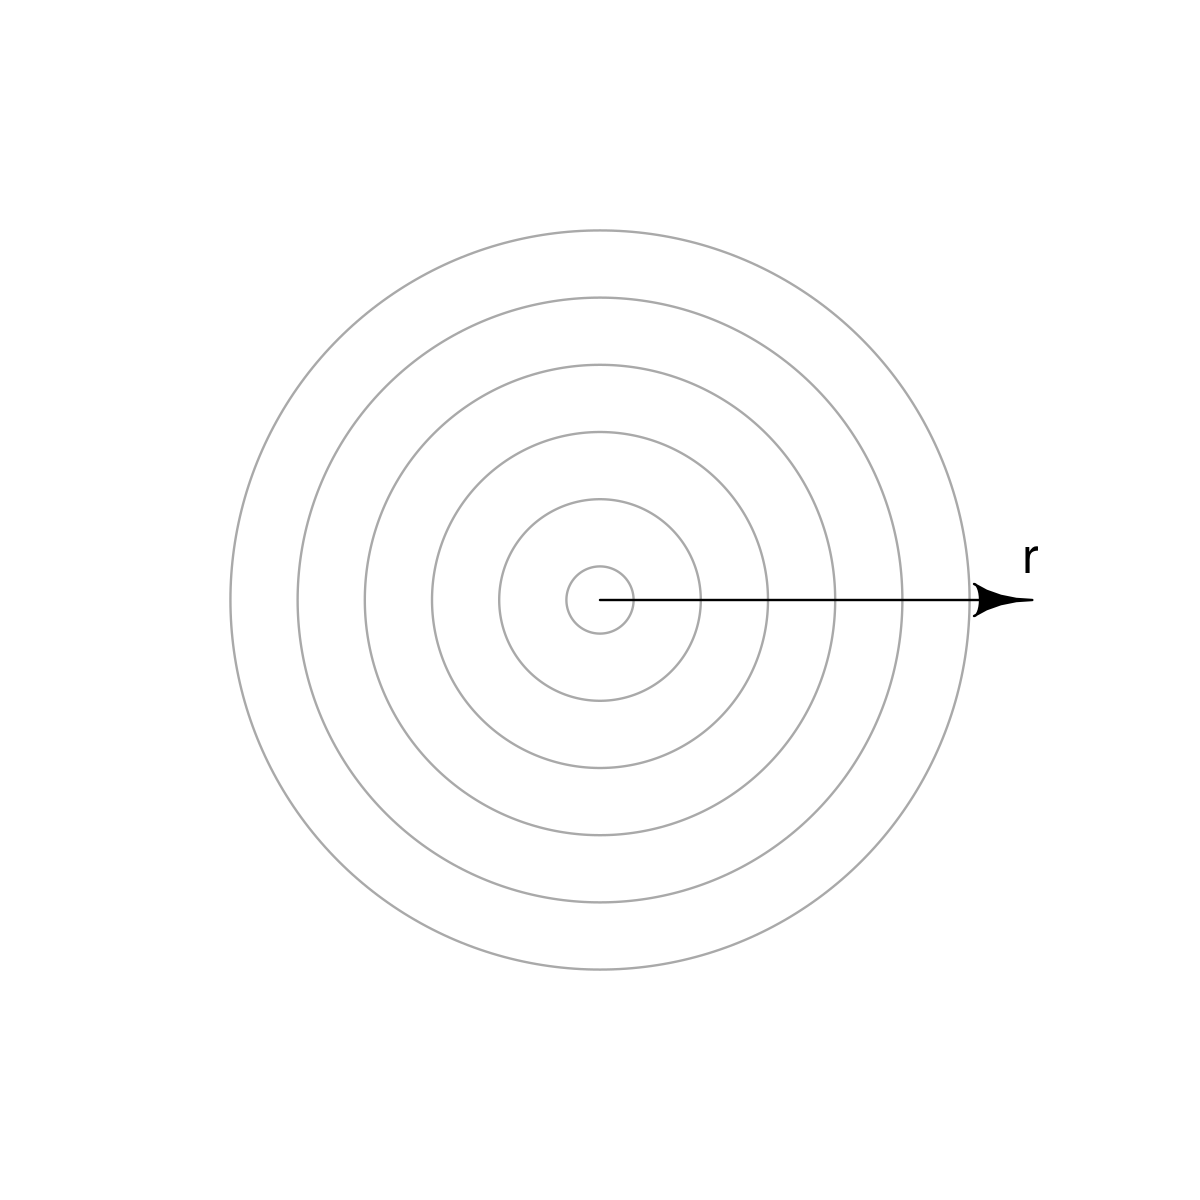
\includegraphics[width=0.4\linewidth]{annular_geom.png}
  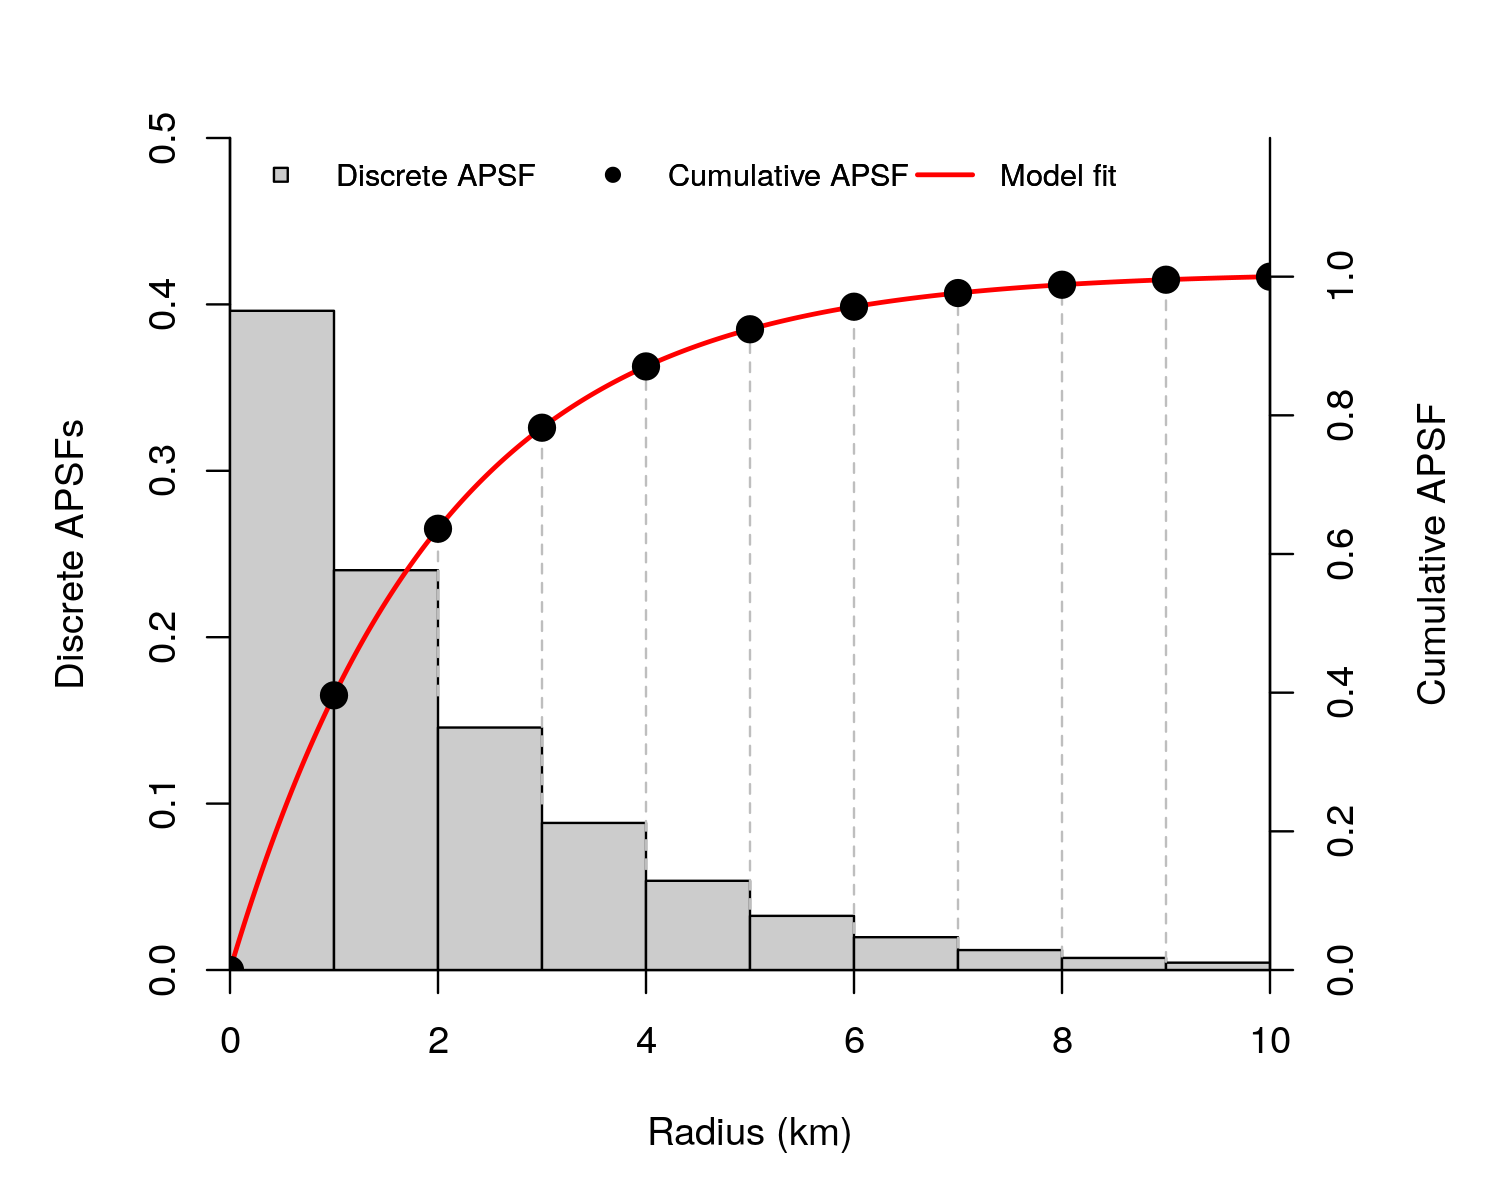
\includegraphics[width=0.5\linewidth]{cumintegral_annular_fit_edu.png}
  \caption{Properties of the annular accumulator geometry for Monte Carlo integrals. (A) A schematic representation of the annular accumulator geometry. (B) A schematic representation of discrete kernel, discrete cumulative distribution function, and model fit.}
  \label{fig:annular_geom}
\end{figure}

Finally, the reconstructed integro-normalised discrete kernel in a grid resolution matching the waveband resolution is scaled when necessary for the magnitude of the process (upward diffuse transmittance for the PSF and spherical albedo for the SAF).

\section{Radiative transfer simulations} 

The radiative transfer simulations for the PSF and SAF kernels are performed in a Backward Monte Carlo radiative transfer code written to support RAdCor, the apsfs library (\url{https://github.com/eoplus/apsfs/}).

Following the system definition in Chapter~\ref{ch:theory}, the Earth-atmosphere system is treated as plane-parallel instead of spherical, with the atmosphere divided in homogeneous layers stacked vertically. For simulations of the spatially resolved spherical albedo, the source (detector) is placed at the bottom of the atmosphere, emitting radiance with a cosine weighted directional function centred at the zenith and covering all directions in the upper hemisphere. For simulations of the atmospheric point spread function, the source (detector) is placed at the nominal height of the sensor, emitting radiance in an infinitesimal solid angle or isotropically within the solid angle defined by the field of view of the detector elements, centred on the viewing direction. The recorded value is the fraction of the emitted radiance received by each surface bin (integration area), that can be defined in an annular, sectorial or grid geometry model. 

The composition and structure of the atmosphere is given by the US standard atmosphere model of 1976 \citep{NOAA1976} and the aerosol optical properties and height distribution are taken from the 6SV radiative transfer model. This was chosen as ACOLITE uses the 6SV aerosol models in its calculations. The optical properties of the atmosphere and its scatter types are shown in Fig.~\ref{fig:sph_albd_sim_saf}.

\begin{figure}[!htbp]
  \centering
  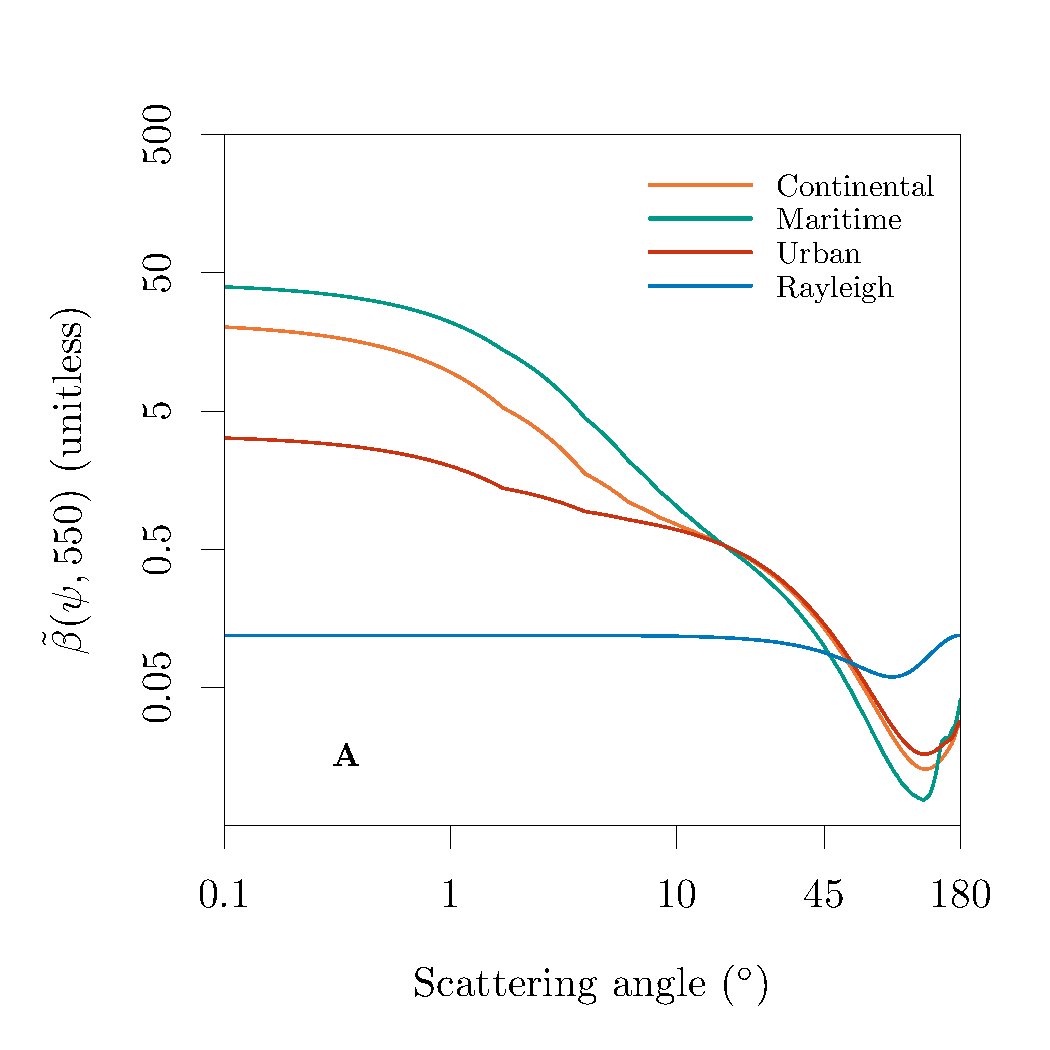
\includegraphics[width=0.45\linewidth]{saf_01_A}
  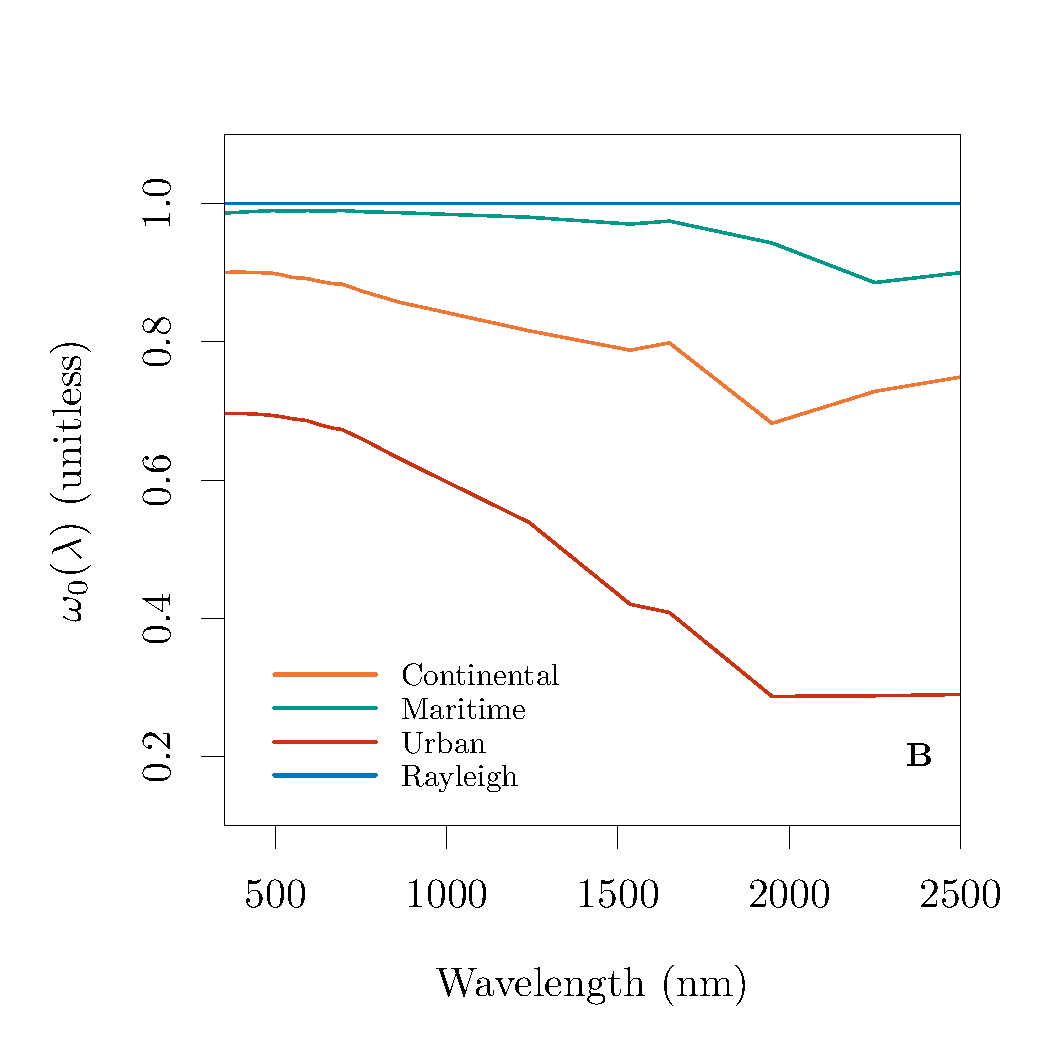
\includegraphics[width=0.45\linewidth]{saf_01_B}
  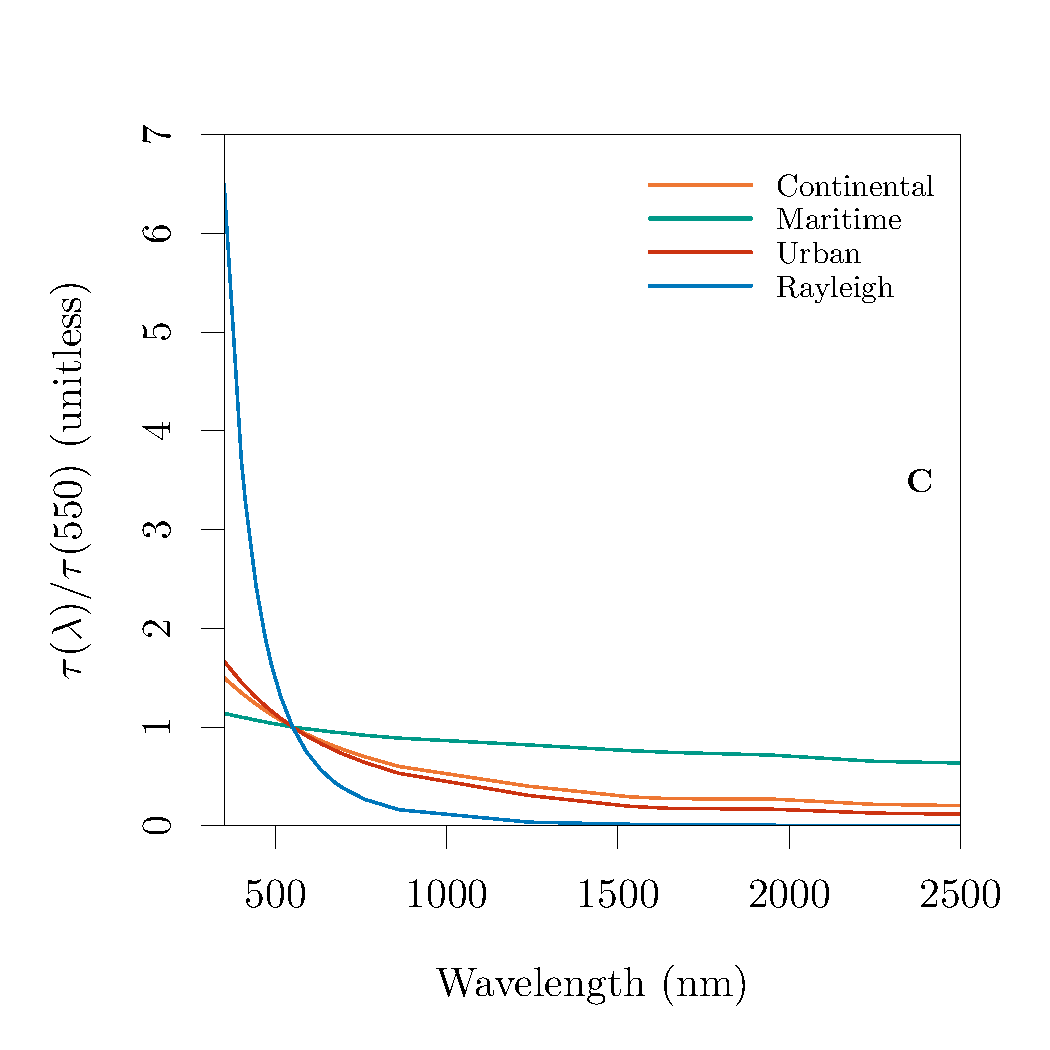
\includegraphics[width=0.45\linewidth]{saf_01_C}
  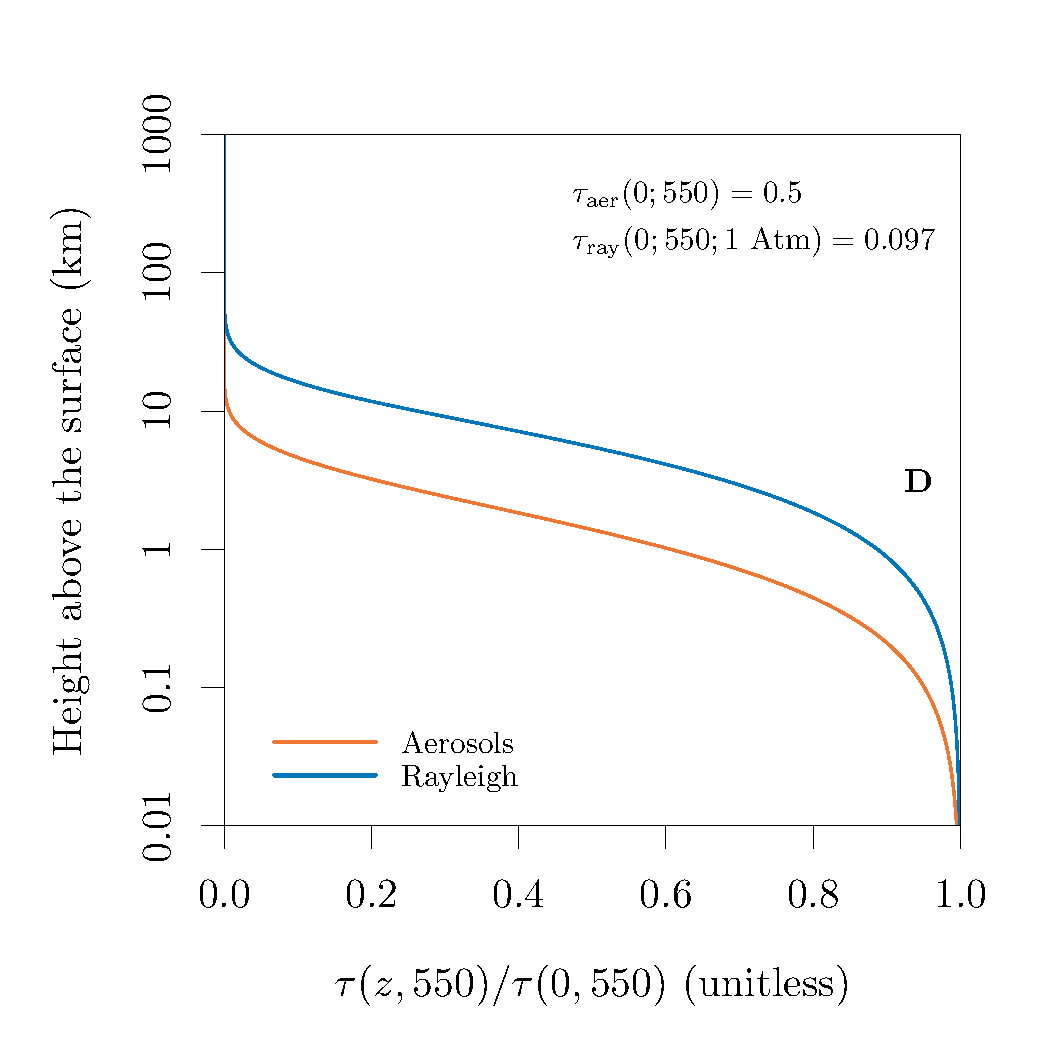
\includegraphics[width=0.45\linewidth]{saf_01_D}
  \caption{Atmospheric properties for radiative transfer simulations. (A) The integro-normalised volume scattering function (scattering phase function) at 550~nm as a function of the scattering angle. (B) The single scattering albedo as a function of wavelength. (C) The optical thickness of the atmosphere as a function of wavelength, normalised by its value at 550~nm. (D) The vertical profile of optical thickness of the atmosphere at 550~nm, as a function of height above the surface, normalised by its value at the surface.}
  \label{fig:sph_albd_sim_saf}
\end{figure}

Simulations were performed with an annular accumulator model, representing the symmetrical condition of near-nadir observation \citep{Reinersman1995}. Idealised atmospheres are used, with only Rayleigh or aerosol scatters, as the calculations for variable combinations of aerosol and Rayleigh can be well approximated by a weighted average of the end member functions, with weights given by their contribution to the spherical albedo. Simulations for aerosol scatters are performed per sensor, taking into account the average height of the orbit above the surface, the spectral response function of the wavebands and the its spatial resolutions. As the Rayleigh scattering phase function and single scattering albedo have no wavelength dependence, simulations are not performed per sensor and waveband, but at four surface pressures: 1100~mbar, 1013.25~mbar, 750~mbar, and 500~mbar, matching the pressure points of the ACOLITE LUTs. Simulations for aerosol scatters were performed at a $\tau_\text{aer} = 0.5$ (unitless), while the simulations for the Rayleigh scatter were performed at the Rayleigh optical thickness at 550~nm for each pressure. Simulations at fixed $\tau$ are expected to be representative of variable $\tau$ as the integro-normalised spatial kernels with the angular integrals of the atmosphere's BSSRDF and BSSTDF depend primarily on the scattering phase function and scattering albedo of the atmosphere and its height distribution.

An indirect validation of the PSF and SAF simulations is provided in Fig.~\ref{fig:sph_albd_sim_val}, comparing the integrated PSF and SAF values with the upward diffuse transmittance and spherical albedo, respectively, calculated with the 6SV radiative transfer model.

\begin{figure}[!htbp]
  \centering
  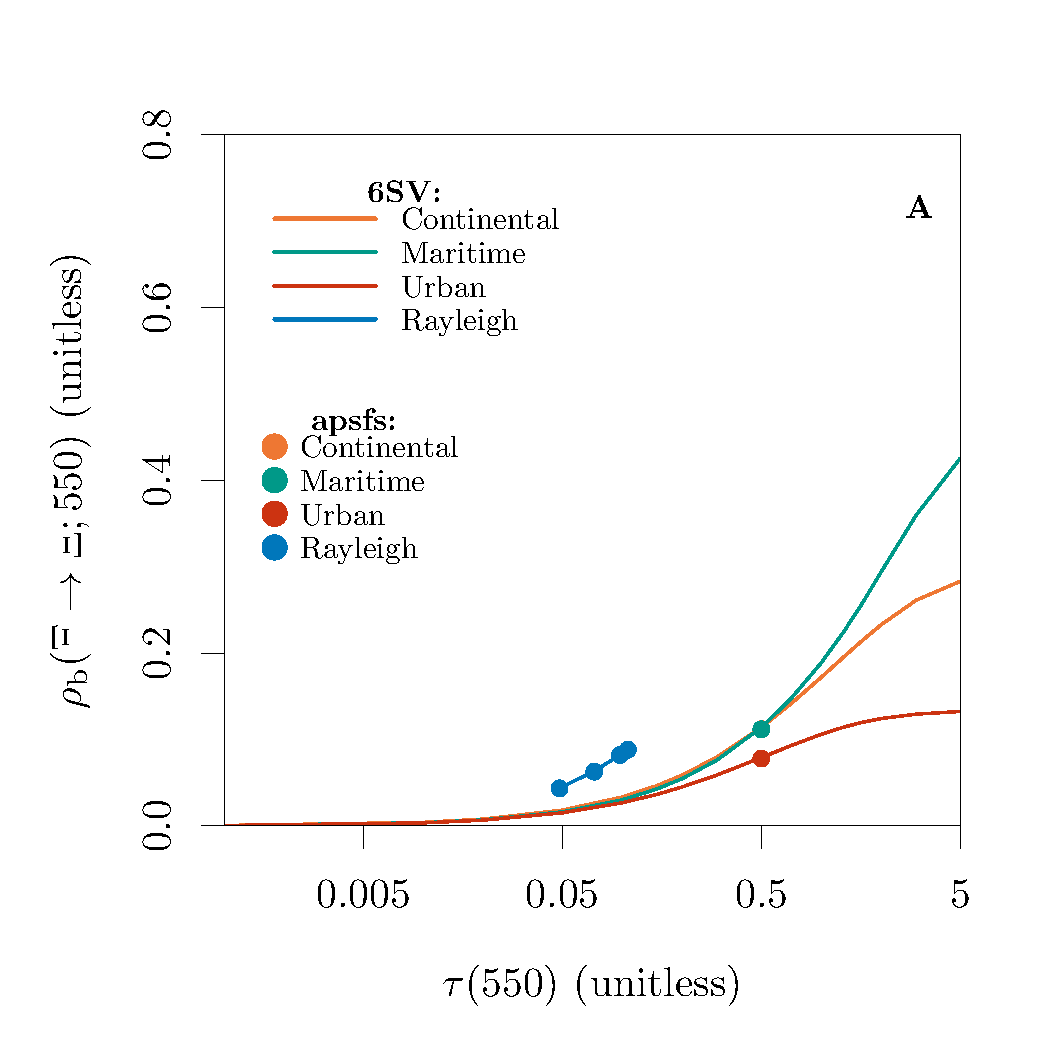
\includegraphics[width=0.45\linewidth]{saf_03_A}
  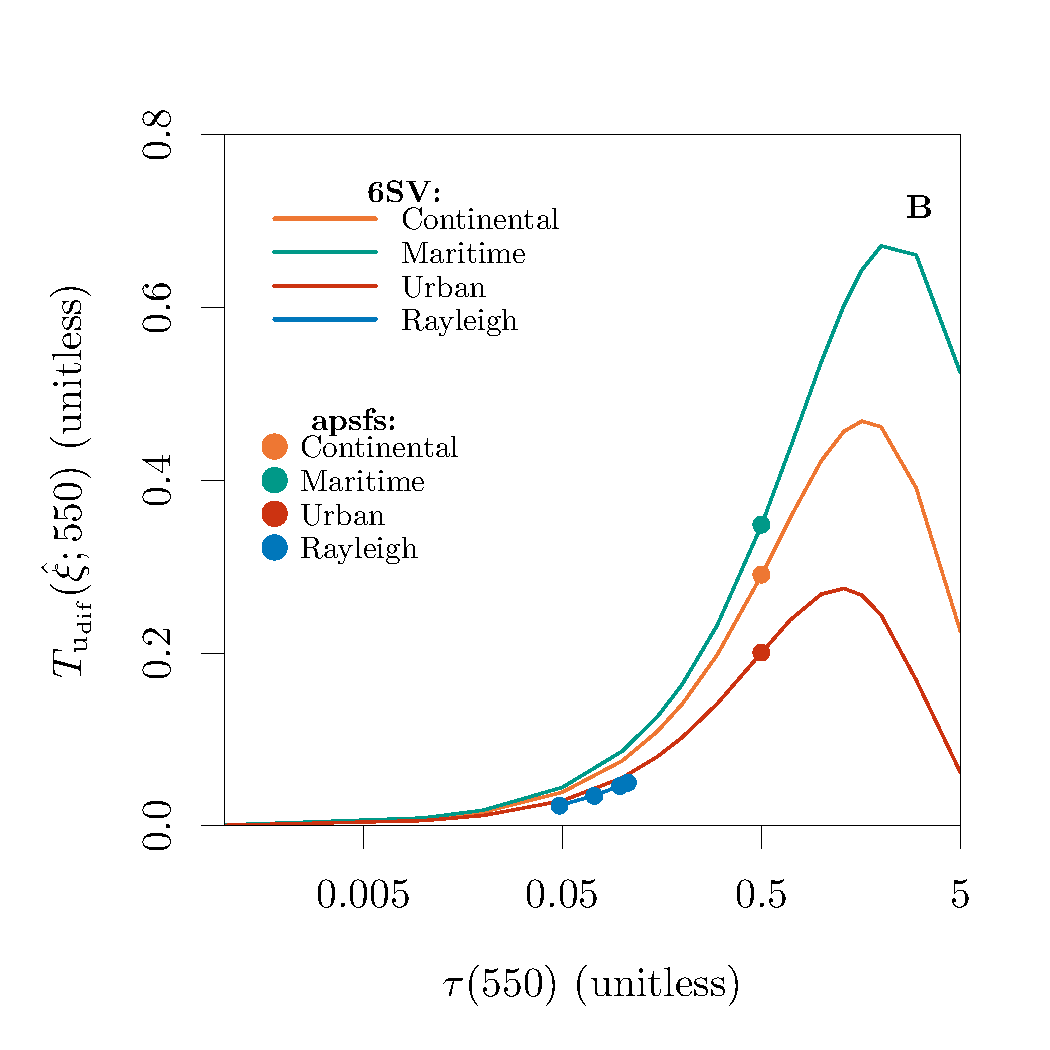
\includegraphics[width=0.45\linewidth]{psf_03_A}
  \caption{Indirect validation of the SAF (A) and PSF (B), by comparing the spherical albedo and upward diffuse transmittance from 6SV and the integral of the SAF and PSF from apsfs.}
  \label{fig:sph_albd_sim_val}
\end{figure}



\end{appendices}

% ------------------------------------------------------------------------------
% Bibliography 
% 

\cleardoublepage
\bibliographystyle{myplainnat}
\bibliography{radcor_D_2_1_ATB}

\end{document}
